% Options for packages loaded elsewhere
\PassOptionsToPackage{unicode}{hyperref}
\PassOptionsToPackage{hyphens}{url}
%
\documentclass[
  11pt,
  letterpaper,
]{book}
\usepackage{lmodern}
\usepackage{amssymb,amsmath}
\usepackage{ifxetex,ifluatex}
\ifnum 0\ifxetex 1\fi\ifluatex 1\fi=0 % if pdftex
  \usepackage[T1]{fontenc}
  \usepackage[utf8]{inputenc}
  \usepackage{textcomp} % provide euro and other symbols
\else % if luatex or xetex
  \usepackage{unicode-math}
  \defaultfontfeatures{Scale=MatchLowercase}
  \defaultfontfeatures[\rmfamily]{Ligatures=TeX,Scale=1}
\fi
% Use upquote if available, for straight quotes in verbatim environments
\IfFileExists{upquote.sty}{\usepackage{upquote}}{}
\IfFileExists{microtype.sty}{% use microtype if available
  \usepackage[]{microtype}
  \UseMicrotypeSet[protrusion]{basicmath} % disable protrusion for tt fonts
}{}
\makeatletter
\@ifundefined{KOMAClassName}{% if non-KOMA class
  \IfFileExists{parskip.sty}{%
    \usepackage{parskip}
  }{% else
    \setlength{\parindent}{0pt}
    \setlength{\parskip}{6pt plus 2pt minus 1pt}}
}{% if KOMA class
  \KOMAoptions{parskip=half}}
\makeatother
\usepackage{xcolor}
\IfFileExists{xurl.sty}{\usepackage{xurl}}{} % add URL line breaks if available
\IfFileExists{bookmark.sty}{\usepackage{bookmark}}{\usepackage{hyperref}}
\hypersetup{
  pdftitle={Statistical Modelling},
  hidelinks,
  pdfcreator={LaTeX via pandoc}}
\urlstyle{same} % disable monospaced font for URLs
\usepackage{color}
\usepackage{fancyvrb}
\newcommand{\VerbBar}{|}
\newcommand{\VERB}{\Verb[commandchars=\\\{\}]}
\DefineVerbatimEnvironment{Highlighting}{Verbatim}{commandchars=\\\{\}}
% Add ',fontsize=\small' for more characters per line
\usepackage{framed}
\definecolor{shadecolor}{RGB}{248,248,248}
\newenvironment{Shaded}{\begin{snugshade}}{\end{snugshade}}
\newcommand{\AlertTok}[1]{\textcolor[rgb]{0.94,0.16,0.16}{#1}}
\newcommand{\AnnotationTok}[1]{\textcolor[rgb]{0.56,0.35,0.01}{\textbf{\textit{#1}}}}
\newcommand{\AttributeTok}[1]{\textcolor[rgb]{0.77,0.63,0.00}{#1}}
\newcommand{\BaseNTok}[1]{\textcolor[rgb]{0.00,0.00,0.81}{#1}}
\newcommand{\BuiltInTok}[1]{#1}
\newcommand{\CharTok}[1]{\textcolor[rgb]{0.31,0.60,0.02}{#1}}
\newcommand{\CommentTok}[1]{\textcolor[rgb]{0.56,0.35,0.01}{\textit{#1}}}
\newcommand{\CommentVarTok}[1]{\textcolor[rgb]{0.56,0.35,0.01}{\textbf{\textit{#1}}}}
\newcommand{\ConstantTok}[1]{\textcolor[rgb]{0.00,0.00,0.00}{#1}}
\newcommand{\ControlFlowTok}[1]{\textcolor[rgb]{0.13,0.29,0.53}{\textbf{#1}}}
\newcommand{\DataTypeTok}[1]{\textcolor[rgb]{0.13,0.29,0.53}{#1}}
\newcommand{\DecValTok}[1]{\textcolor[rgb]{0.00,0.00,0.81}{#1}}
\newcommand{\DocumentationTok}[1]{\textcolor[rgb]{0.56,0.35,0.01}{\textbf{\textit{#1}}}}
\newcommand{\ErrorTok}[1]{\textcolor[rgb]{0.64,0.00,0.00}{\textbf{#1}}}
\newcommand{\ExtensionTok}[1]{#1}
\newcommand{\FloatTok}[1]{\textcolor[rgb]{0.00,0.00,0.81}{#1}}
\newcommand{\FunctionTok}[1]{\textcolor[rgb]{0.00,0.00,0.00}{#1}}
\newcommand{\ImportTok}[1]{#1}
\newcommand{\InformationTok}[1]{\textcolor[rgb]{0.56,0.35,0.01}{\textbf{\textit{#1}}}}
\newcommand{\KeywordTok}[1]{\textcolor[rgb]{0.13,0.29,0.53}{\textbf{#1}}}
\newcommand{\NormalTok}[1]{#1}
\newcommand{\OperatorTok}[1]{\textcolor[rgb]{0.81,0.36,0.00}{\textbf{#1}}}
\newcommand{\OtherTok}[1]{\textcolor[rgb]{0.56,0.35,0.01}{#1}}
\newcommand{\PreprocessorTok}[1]{\textcolor[rgb]{0.56,0.35,0.01}{\textit{#1}}}
\newcommand{\RegionMarkerTok}[1]{#1}
\newcommand{\SpecialCharTok}[1]{\textcolor[rgb]{0.00,0.00,0.00}{#1}}
\newcommand{\SpecialStringTok}[1]{\textcolor[rgb]{0.31,0.60,0.02}{#1}}
\newcommand{\StringTok}[1]{\textcolor[rgb]{0.31,0.60,0.02}{#1}}
\newcommand{\VariableTok}[1]{\textcolor[rgb]{0.00,0.00,0.00}{#1}}
\newcommand{\VerbatimStringTok}[1]{\textcolor[rgb]{0.31,0.60,0.02}{#1}}
\newcommand{\WarningTok}[1]{\textcolor[rgb]{0.56,0.35,0.01}{\textbf{\textit{#1}}}}
\usepackage{longtable,booktabs}
% Correct order of tables after \paragraph or \subparagraph
\usepackage{etoolbox}
\makeatletter
\patchcmd\longtable{\par}{\if@noskipsec\mbox{}\fi\par}{}{}
\makeatother
% Allow footnotes in longtable head/foot
\IfFileExists{footnotehyper.sty}{\usepackage{footnotehyper}}{\usepackage{footnote}}
\makesavenoteenv{longtable}
\usepackage{graphicx}
\makeatletter
\def\maxwidth{\ifdim\Gin@nat@width>\linewidth\linewidth\else\Gin@nat@width\fi}
\def\maxheight{\ifdim\Gin@nat@height>\textheight\textheight\else\Gin@nat@height\fi}
\makeatother
% Scale images if necessary, so that they will not overflow the page
% margins by default, and it is still possible to overwrite the defaults
% using explicit options in \includegraphics[width, height, ...]{}
\setkeys{Gin}{width=\maxwidth,height=\maxheight,keepaspectratio}
% Set default figure placement to htbp
\makeatletter
\def\fps@figure{htbp}
\makeatother
\setlength{\emergencystretch}{3em} % prevent overfull lines
\providecommand{\tightlist}{%
  \setlength{\itemsep}{0pt}\setlength{\parskip}{0pt}}
\setcounter{secnumdepth}{5}
% \usepackage{amsmath,amssymb,mathtools}
\usepackage{enumerate}
\usepackage{geometry}
\geometry{hmargin=1.2in}

\usepackage{booktabs}
\usepackage{amssymb}
\makeatletter
\def\thm@space@setup{%
  \thm@preskip=8pt plus 2pt minus 4pt
  \thm@postskip=\thm@preskip
}
\makeatother

\usepackage{framed,color}
\definecolor{shadecolor}{RGB}{248,248,248}

\renewcommand{\textfraction}{0.05}
\renewcommand{\topfraction}{0.8}
\renewcommand{\bottomfraction}{0.8}
\renewcommand{\floatpagefraction}{0.75}

\let\oldhref\href
\renewcommand{\href}[2]{#2\footnote{\url{#1}}}

\ifxetex
  \usepackage{letltxmacro}
  \setlength{\XeTeXLinkMargin}{1pt}
  \LetLtxMacro\SavedIncludeGraphics\includegraphics
  \def\includegraphics#1#{% #1 catches optional stuff (star/opt. arg.)
    \IncludeGraphicsAux{#1}%
  }%
  \newcommand*{\IncludeGraphicsAux}[2]{%
    \XeTeXLinkBox{%
      \SavedIncludeGraphics#1{#2}%
    }%
  }%
\fi

\makeatletter
\newenvironment{kframe}{%
\medskip{}
\setlength{\fboxsep}{.8em}
 \def\at@end@of@kframe{}%
 \ifinner\ifhmode%
  \def\at@end@of@kframe{\end{minipage}}%
  \begin{minipage}{\columnwidth}%
 \fi\fi%
 \def\FrameCommand##1{\hskip\@totalleftmargin \hskip-\fboxsep
 \colorbox{shadecolor}{##1}\hskip-\fboxsep
     % There is no \\@totalrightmargin, so:
     \hskip-\linewidth \hskip-\@totalleftmargin \hskip\columnwidth}%
 \MakeFramed {\advance\hsize-\width
   \@totalleftmargin\z@ \linewidth\hsize
   \@setminipage}}%
 {\par\unskip\endMakeFramed%
 \at@end@of@kframe}
\makeatother

\makeatletter
\@ifundefined{Shaded}{
}{\renewenvironment{Shaded}{\begin{kframe}}{\end{kframe}}}
\makeatother

\newenvironment{rmdblock}[1]
  {
  \begin{itemize}
  \renewcommand{\labelitemi}{
    \raisebox{-.7\height}[0pt][0pt]{
      {\setkeys{Gin}{width=3em,keepaspectratio}\includegraphics{images/#1}}
    }
  }
  \setlength{\fboxsep}{1em}
  \begin{kframe}
  \item
  }
  {
  \end{kframe}
  \end{itemize}
  }
\newenvironment{rmdnote}
  {\begin{rmdblock}{note}}
  {\end{rmdblock}}
\newenvironment{rmdcaution}
  {\begin{rmdblock}{caution}}
  {\end{rmdblock}}
\newenvironment{rmdimportant}
  {\begin{rmdblock}{important}}
  {\end{rmdblock}}
\newenvironment{rmdtip}
  {\begin{rmdblock}{tip}}
  {\end{rmdblock}}
\newenvironment{rmdwarning}
  {\begin{rmdblock}{warning}}
  {\end{rmdblock}}
\usepackage{mathrsfs}
\DeclareMathAlphabet{\mathcrl}{U}{rsfs}{m}{n}
\usepackage{utopia}
\DeclareMathAlphabet{\mathcal}{OMS}{cmsy}{m}{n}
\ifluatex
  \usepackage{selnolig}  % disable illegal ligatures
\fi
\usepackage[]{natbib}
\bibliographystyle{apalike2}

\title{Statistical Modelling}
\author{}
\date{\vspace{-2.5em}}

\usepackage{amsthm}
\newtheorem{theorem}{Theorem}[chapter]
\newtheorem{lemma}{Lemma}[chapter]
\newtheorem{corollary}{Corollary}[chapter]
\newtheorem{proposition}{Proposition}[chapter]
\newtheorem{conjecture}{Conjecture}[chapter]
\theoremstyle{definition}
\newtheorem{definition}{Definition}[chapter]
\theoremstyle{definition}
\newtheorem{example}{Example}[chapter]
\theoremstyle{definition}
\newtheorem{exercise}{Exercise}[chapter]
\theoremstyle{remark}
\newtheorem*{remark}{Remark}
\newtheorem*{solution}{Solution}
\begin{document}
\maketitle

\let\href\oldhref

{
\setcounter{tocdepth}{1}
\tableofcontents
}
\hypertarget{preliminary-remarks}{%
\chapter*{Preliminary remarks}\label{preliminary-remarks}}
\addcontentsline{toc}{chapter}{Preliminary remarks}

These notes by Léo Belzile (HEC Montréal) are licensed under a \href{http://creativecommons.org/licenses/by-nc-sa/4.0/}{Creative Commons Attribution-NonCommercial-ShareAlike 4.0 International License} and were last compiled on 2020-10-18.

While we show how to implement statistical tests and models in \textbf{SAS} in class, these note will illustrate the concepts using \textbf{R}: visit \href{https://cran.r-project.org/}{the R-project website} to download the program. The most popular graphical cross-platform front-end is \href{https://www.rstudio.com/products/rstudio/download/}{RStudio Desktop}.

The most famous quote about statistical models is probably due to George Box, who claimed that ``all models are wrong, but some are useful''. This standpoint is reductive: Peter McCullagh and John Nelder wrote in the preamble of their book (emphasis mine)

\begin{quote}
Modelling in science remains, partly at least, an art. Some principles do exist, however, to guide the modeller. The first is that all models are wrong; \textbf{some, though, are better} than others and we can \textbf{search for the better ones}. At the same time we must recognize that eternal truth is not within our grasp.
\end{quote}

And this quote by David R. Cox adds to the point:

\begin{quote}
\ldots it does not seem helpful just to say that all models are wrong. The very word model implies simplification and idealization. The idea that com-
plex physical, biological or sociological systems can be exactly described
by a few formulae is patently absurd. The construction of idealized representations that \textbf{capture important stable aspects of such systems}
is, however, a vital part of general scientific analysis and statistical models, especially substantive ones, do not seem essentially different from
other kinds of model.
\end{quote}

\newcommand{\bs}[1]{\boldsymbol{#1}}
\newcommand{\Hmat}{\mathbf{H}}
\newcommand{\Mmat}{\mathbf{M}}
\newcommand{\mX}{\mathbf{X}}
\newcommand{\bX}{{\mathbf{X}}}
\newcommand{\bx}{{\mathbf{x}}}
\newcommand{\by}{{\boldsymbol{y}}}
\newcommand{\bY}{{\boldsymbol{Y}}}
\newcommand{\eps}{\varepsilon}
\newcommand{\beps}{\boldsymbol{\varepsilon}}
\newcommand{\bbeta}{\boldsymbol{\beta}}
\newcommand{\hbb}{\hat{\boldsymbol{\beta}}}
\newcommand{\limni}{\lim_{n \ra \infty}}
\newcommand{\Sp}{\mathscr{S}}
\newcommand{\Hy}{\mathscr{H}}
\newcommand{\E}[2][]{{\mathsf E}_{#1}\left(#2\right)}
\newcommand{\Va}[2][]{{\mathsf{Var}_{#1}}\left(#2\right)}
\newcommand{\I}[1]{{\mathbf 1}_{#1}}

\hypertarget{intro}{%
\chapter{Introduction to statistical inference}\label{intro}}

Statistical modelling requires a good graps of statistical inference: as such, we begin with a review of hypothesis testing and graphical exploratory data analysis.

The purpose of statistical inference is to draw conclusions based on data. Scientific research relies on hypothesis testing: once an hypothesis is formulated, the researcher collects data, performs a test and concludes as to whether there is evidence for the proposed theory.

There are two main data type: \textbf{experimental} data are typically collected in a control environment following a research protocol with a particular experimental design: they serve to answer questions specified ahead of time. This approach is highly desirable to avoid the garden of forking paths \href{http://www.stat.columbia.edu/~gelman/research/unpublished/p_hacking.pdf}{(researchers unfortunately tend to refine or change their hypothesis in light of data, which invalidates their findings} --- preregistration alleviates this somewhat). While experimental data are highly desirable, it is not always possible to collect experimental data: for example, an economist cannot modify interest rates to see how it impacts consumer savings. When data have been collected beforehand without intervention (for other purposes), these are called \textbf{observational}. These will be the ones most frequently encountered.

A stochastic model will comprise two ingredients: a distribution for the random data and a formula linking the parameters or the conditional expectation of a response variable \(Y\) to a set of explanatories \(\mathbf{X}\). A model can serve to either predict new outcomes (predictive modelling) or else to test research hypothesis about the effect of the explanatory variables on the response (explanatory model). These two objectives are of course not mutually exclusive even if we distinguish in practice inference and prediction.

A predictive model gives predictions of \(Y\) for different combinations of explanatory variables or future data. For example, one could try to forecast the enery consumption of a house as a function of weather, the number of inhabitants and its size. Black boxes used in machine learning are often used solely for prediction: these models are not easily interpreted and they often ignore the data structure.

By constrast, explicative models are often simple and interpretable: regression models are often used for inference purpose and we will focus on these.

\begin{itemize}
\tightlist
\item
  Are consumer ready to spend more when they pay by credit card rather than by cash?
\item
  Is there wage discrimination towards women in a US college?
\item
  University degree: \href{https://www.theglobeandmail.com/report-on-business/is-the-university-experience-worth-the-cost/article31703109/}{``is the university experience worth the cost'\,'?}
\item
  What are the criteria impacting health insurance premiums?
\item
  Is the price of gasoline more expansive in the Gaspé peninsula than in the rest of Quebec? \href{http://www.regie-energie.qc.ca/energie/rapports/Rapport_priceGasp\%C3\%A9sie_20191219.pdf}{A report of the \emph{Régie de l'énergie} examines the question}
\item
  Are driving tests in the UK easier if you live in a rural area? \href{https://www.theguardian.com/world/2019/aug/23/an-easy-ride-scottish-village-fuels-debate-driving-test-pass-rates}{An analysis of \emph{The Guardian}} hints that it is the case.
\item
  Does the risk of transmission of Covid19 increase with distancing? \href{https://www.thelancet.com/journals/lancet/article/PIIS0140-6736(20)31142-9/fulltext}{A (bad) meta-analysis says two meters is better than one} (or how to draw erroneous conclusions from a bad model).
\end{itemize}

\hypertarget{tests}{%
\section{Hypothesis testing}\label{tests}}

An hypothesis test is a binary decision rule used to evaluate the statistical evidence provided by a sample to make a decision regarding the underlying population. The main steps involved are:

\begin{itemize}
\tightlist
\item
  define the model parameters
\item
  formulate the alternative and null hypothesis
\item
  choose and calculate the test statistic
\item
  obtain the null distribution describing the behaviour of the test statistic under \(\mathscr{H}_0\)
\item
  calculate the \emph{p}-value
\item
  conclude (reject or fail to reject \(\mathscr{H}_0\)) in the context of the problem.
\end{itemize}

A good analogy for hypothesis tests is a trial for murder on which you are appointed juror.

\begin{itemize}
\tightlist
\item
  The judge lets you choose between two mutually exclusive outcome, guilty or not guilty, based on the evidence presented in court.
\item
  The presumption of innocence applies and evidences are judged under this optic: are evidence remotely plausible if the person was innocent? The burden of the proof lies with the prosecution to avoid as much as possible judicial errors. The null hypothesis \(\mathscr{H}_0\) is \emph{not guilty}, whereas the alternative \(\mathscr{H}_a\) is \emph{guilty}. If there is a reasonable doubt, the verdict of the trial will be not guilty.
\item
  The test statistic (and the choice of test) represents the summary of the proof. The more overwhelming the evidence, the higher the chance the accused will be declared guilty. The prosecutor chooses the proof so as to best outline this: the choice of evidence (statistic) ultimately will maximise the evidence, which parallels the power of the test.
\item
  The final step is the verdict. This is a binary decision, guilty or not guilty. For an hypothesis test performed at level \(\alpha\), one would reject (guilty) if the \emph{p}-value is less than \(\alpha\).
\end{itemize}

The above description provides some heuristic, but lack crucial details developed in the next section written by Juliana Schulz.

\hypertarget{hypothesis}{%
\subsection{Hypothesis}\label{hypothesis}}

In statistical tests we have two hypotheses: the null hypothesis (\(H_0\)) and the alternative hypothesis (\(H_1\)). Usually, the null hypothesis is the `status quo' and the alternative is what we're really interested in testing. A statistical hypothesis test allows us to decide whether or not our data provides enough evidence to reject \(H_0\) in favour of \(H_1\), subject to some pre-specified risk of error. Usually, hypothesis tests involve a parameter, say \(\theta\), which characterizes the underlying distribution at the population level ans whose value is unknown. A two-sided hypothesis test regarding a parameter \(\theta\) has the form
\begin{align*}
\mathscr{H}_0: \theta=\theta_0 \qquad \text{versus} \qquad \mathscr{H}_a:\theta \neq \theta_0.
\end{align*}
We are testing whether or not \(\theta\) is precisely equal to the value \(\theta_0\). The hypotheses are a statistical representation of our research question.

For example, for a two-sided test for the regression coefficient \(\beta_j\) associated to an explanatory variable \(\mathrm{X}_j\), the null and alternative hypothesis are
explicative d'intérêt \(\mathrm{X}_j\), les hypothèses sont
\begin{align*}
\mathscr{H}_0: \beta_j=\beta_j^0 \qquad \text{versus} \qquad \mathscr{H}_a:\beta_j \neq \beta_j^0, 
\end{align*}
where \(\beta_j^0\) is some value that reflects the research question of interest. For example, if \(\beta_j^0=0\), the underlying question is: is covariate \(\mathrm{X}_j\) impacting the response \(Y\) once other variables have been taken into account?

Note that we can impose direction in the hypotheses and consider alternatives of the form \(\mathscr{H}_a: \theta > \theta_0\) or \(\mathscr{H}_a: \theta < \theta_0\).

\hypertarget{test-statistic}{%
\subsection{Test statistic}\label{test-statistic}}

A test statistic \(T\) is a functional of the data that summarise the information contained in the sample for \(\theta\). The form of the test statistic is chosen such that we know its underlying distribution under \(H_0\), that is, the potential values taken by \(T\) and their relative probability if \(H_0\) is true. Indeed, \(Y\) is a random variable and its value change from one sample to the next.
This allows us to determine what values of \(T\) are likely if \(H_0\) is true. Many statistics we will consider are \textbf{Wald statistic}, of the form
\begin{align*}
T = \frac{\widehat{\theta} - \theta_0}{\mathrm{se}(\widehat{\theta})} 
\end{align*}
where \(\widehat{\theta}\) is an estimator of \(\theta\), \(\theta_0\) is the postulated value of the parameter and \(\mathrm{se}(\widehat{\theta})\) is an estimator of the standard deviation of the test statistic \(\widehat{\theta}\).

For example, to test whether the mean of a population is zero, we set
\begin{align*}
\mathscr{H}_0: \mu=0, \qquad  \mathscr{H}_a:\mu \neq 0, 
\end{align*}
and the Wald statistic is
\begin{align*}
T &= \frac{\overline{X}-0}{S_n/\sqrt{n}}
\end{align*}
where \(\overline{X}\) is the sample mean of \(X_1, \ldots, X_n\),
\begin{align*}
\overline{X} &= \frac{1}{n} \sum_{i=1}^n X_i = \frac{X_1+ \cdots + X_n}{n}
\end{align*}
and the standard error (of the mean) \(\overline{X}\) is \(S_n/\sqrt{n}\); the sample variance \(S_n\) is an estimator of the standard deviation \(\sigma\),
\begin{align*}
S^2_n &= \frac{1}{n-1} \sum_{i=1}^n (X_i-\overline{X})^2.
\end{align*}

Its important to distinguish between procedures/formulas and their numerical values. An \textbf{estimator} is a rule or formula used to calculate an estimate of some parameter or quantity of interest based on observed data. For example, the sample mean \(\bar{X}\) is an estimator of the population mean \(\mu\). Once we have observed data we can actually compute the sample mean, that is, we have an estimate --- an actual value. In other words,

\begin{itemize}
\tightlist
\item
  an estimator is the procedure or formula telling us how to use sample data to compute an estimate. Its a random variable since it depends on the sample.
\item
  an estimate is the numerical value obtained once we apply the formula to observed data
\end{itemize}

\hypertarget{null-distribution-and-p-value}{%
\subsection{\texorpdfstring{Null distribution and \emph{p}-value}{Null distribution and p-value}}\label{null-distribution-and-p-value}}

The \emph{p}-value allows us to decide whether the observed value of the test statistic \(T\) is plausible under \(H_0\). Specifically, the \emph{p}-value is the probability that the test statistic is equal or more extreme to the estimate computed from the data, assuming \(H_0\) is true. Suppose that based on a random sample \(X_1, \ldots, X_n\) we obtain a statistic whose value \(T=t\). For a two-sided test \(\mathscr{H}_0:\theta=\theta_0\) vs.~\(\mathscr{H}_a:\theta \neq \theta_0\), the \emph{p}-value is \(\mathsf{Pr}_0(|T| \geq |t|)\). If the distribution of \(T\) is symmetric around zero, the \emph{p}-value is
\begin{align*}
p = 2 \times \mathsf{Pr}_0(T \geq |t|).
\end{align*}

Consider the example of a two-sided test involving the population mean \(H_0:\mu=0\) against the alternative \(H_1:\mu \neq 0\). Assuming the random sample comes from a normal (population) \(\mathsf{No}(\mu, \sigma^2)\), it can be shown that if \(H_0\) is true (that is, if \(\mu=0\)), the test statistic
\begin{align*}
T = \frac{\overline{X}}{S/\sqrt{n}}
\end{align*}
follows a Student-\emph{t} distribution with \(n-1\) degrees of freedom, denoted \(\mathsf{St}_{n-1}\). This allows us to calculate the \emph{p}-value (either from a table, or using some statistical software). The Student-\emph{t} distribution is symmetric about zero, so the \emph{p}-value is \(P = 2\times\mathsf{Pr}(T_{n-1} > |t|)\), where \(T \sim \mathsf{St}_{n-1}\).

\hypertarget{conclusion}{%
\subsection{Conclusion}\label{conclusion}}

The \emph{p}-value allows us to make a decision about the null hypothesis. If \(\mathscr{H}_0\) is true, the \emph{p}-value follows a uniform distribution. \href{https://xkcd.com/1478/}{Thus, if the \emph{p}-value is small}, this means observing an outcome more extreme than \(T=t\) is unlikely, and so we're inclined to think that \(H_0\) is not true. There's always some underlying risk that we're making a mistake when we make a decision. In statistic, there are \href{https://xkcd.com/2303/}{two type of errors}:

\begin{itemize}
\tightlist
\item
  type I error: we reject \(H_0\) when \(H_0\) is true,
\item
  type II error: we fail to reject \(H_0\) when \(H_0\) is false.
\end{itemize}

These hypothesis are not judged equally: we seek to avoid error of type I (judicial errors, corresponding to condamning an innocent). To prevent this, we fix a the level of the test, \(\alpha\), which captures our tolerance to the risk of commiting a type I error: the higher the level of the test \(\alpha\), the more often we will reject the null hypothesis when the latter is true. The value of \(\alpha \in (0, 1)\) is the probability of rejecting \(\mathscr{H}_0\) when \(\mathscr{H}_0\) is in fact true,
\begin{align*}
\alpha = \mathsf{Pr}_0\left(\text{ reject } \mathscr{H}_0\right).
\end{align*}
The level \(\alpha\) is fixed beforehand, typically \(1\)\%, \(5\)\% or \(10\)\%. Keep in mind that the probability of type I error is \(\alpha\) only if the null model for \(\mathscr{H}_0\) is correct (sic) and correspond to the data generating mechanism.

The focus on type I error is best understood by thinking about medical trial: you need to prove a new cure is better than existing alternatives drugs or placebo, to avoid extra costs or harming patients (think of Didier Raoult and his unsubstantiated claims that hydrochloroquine, an antipaludean drug, should be recommended treatment against Covid19).

\begin{longtable}[]{@{}lcc@{}}
\toprule
\textbf{Decision} \textbackslash{} \textbf{true model} & \(\mathscr{H}_0\) & \(\mathscr{H}_a\)\tabularnewline
\midrule
\endhead
fail to reject \(\mathscr{H}_0\) & \(\checkmark\) & type II error\tabularnewline
reject \(\mathscr{H}_0\) & type I error & \(\checkmark\)\tabularnewline
\bottomrule
\end{longtable}

To make a decision, we compare our \emph{p}-value \(P\) with the level of the test \(\alpha\):

\begin{itemize}
\tightlist
\item
  if \(P < \alpha\), we reject \(\mathscr{H}_0\);
\item
  if \(P \geq \alpha\), we fail to reject \(\mathscr{H}_0\).
\end{itemize}

Do not mix up level of the test (probability fixed beforehand by the researcher) and the \emph{p}-value. If you do a test at level 5\%, the probability of type I error is by definition \(\alpha\) and does not depend on the \emph{p}-value. The latter is conditional probability of observing a more extreme likelihood given the null distribution \(\mathscr{H}_0\) is true.

\hypertarget{power}{%
\subsection{Power}\label{power}}

There are two sides to an hypothesis test: either we want to show it is not unreasonable to assume the null hypothesis, or else we want to show beyond reasonable doubt that a difference or effect is significative: for example, one could wish to demonstrate that a new website design (alternative hypothesis) leads to a significant increase in sales relative to the status quo. Our ability to detect these improvements and make discoveries depends on the power of the test: the larger the power, the greater our ability to reject \(\mathscr{H}_0\) when the latter is false.

Failing to reject \(\mathscr{H}_0\) when \(\mathscr{H}_a\) is true corresponds to the definition of type II error, the probability of which is \(1-\gamma\), say. The \textbf{power of a test} is the probability of rejecting \(\mathscr{H}_0\) when \(\mathscr{H}_0\) is false, i.e.,
\begin{align*}
\gamma = \mathsf{Pr}_a(\text{reject} \mathscr{H}_0)
\end{align*}
Depending on the alternative models, it is more or less easy to detect that the null hypothesis is false and reject in favor of an alternative.

\begin{figure}

{\centering 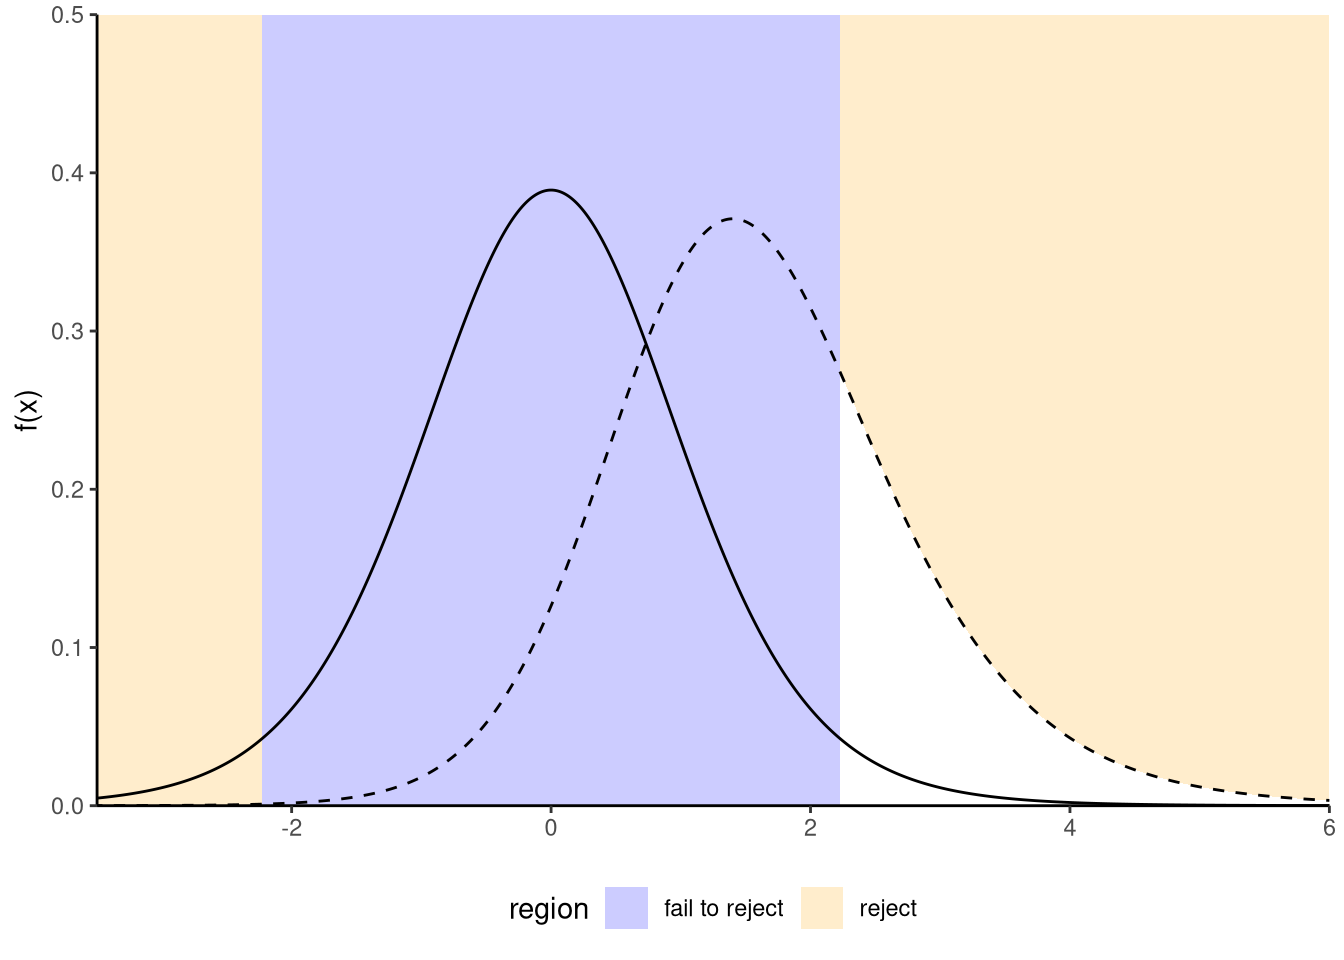
\includegraphics[width=0.7\linewidth]{MATH60604A_Statistical_modelling_files/figure-latex/power1-1} 

}

\caption{Comparison between null distribution (full curve) and a specific alternative for a *t*-test (dashed line). The power corresponds to the area under the curve of the density of the alternative distribution which is in the rejection area (in white).}\label{fig:power1}
\end{figure}

\begin{figure}

{\centering 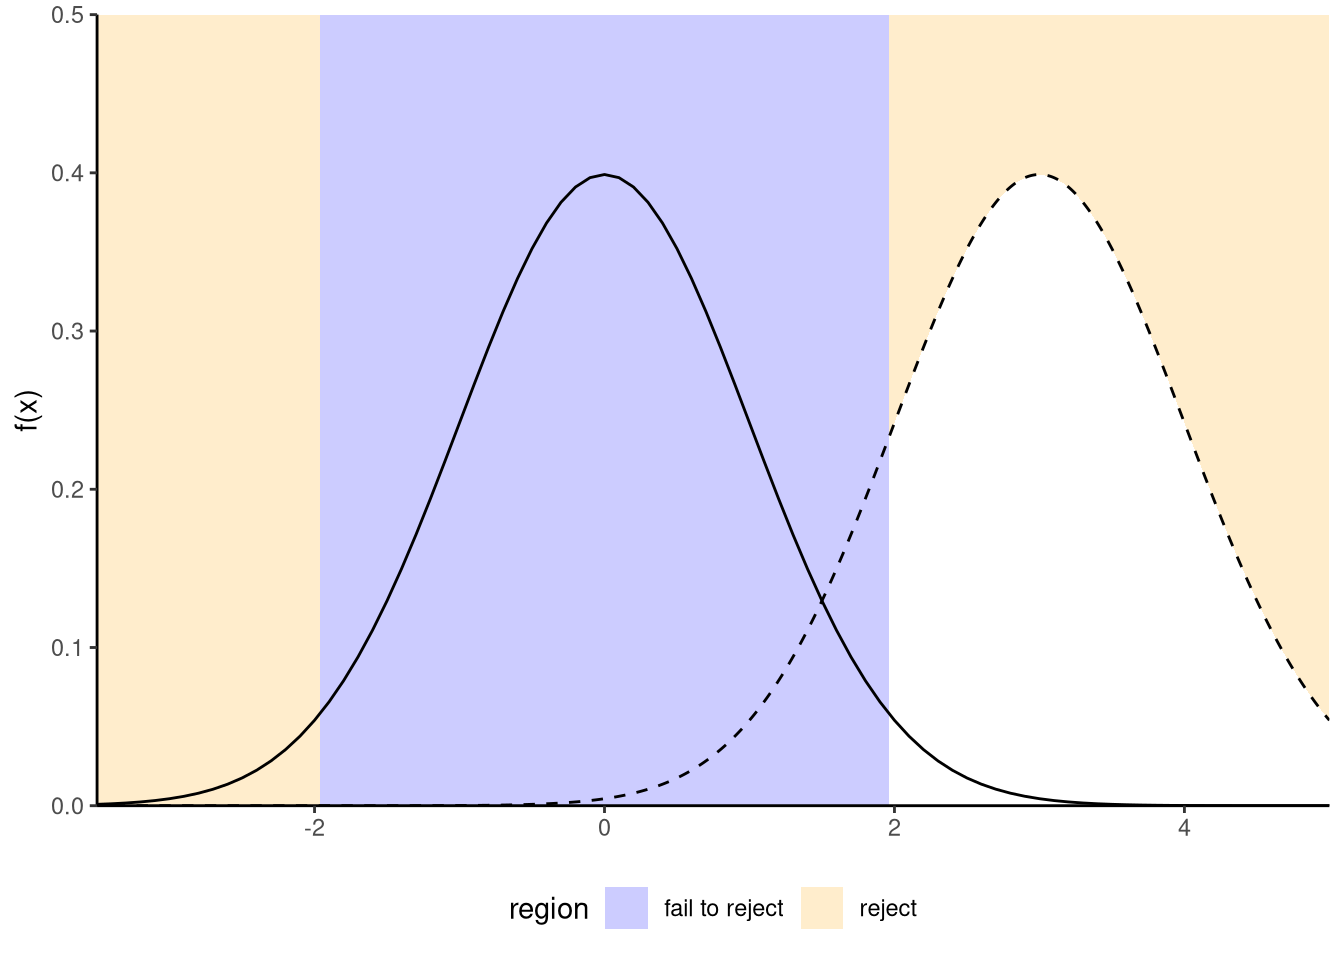
\includegraphics[width=0.7\linewidth]{MATH60604A_Statistical_modelling_files/figure-latex/power2-1} 

}

\caption{Increase in power due to an increase in the mean difference between the null and alternative hypothesis. Power is the area in the rejection region (in white) under the alternative distribution (dashed): the latter is more shifted to the right relative to the null distribution (full line).}\label{fig:power2}
\end{figure}

\begin{figure}

{\centering 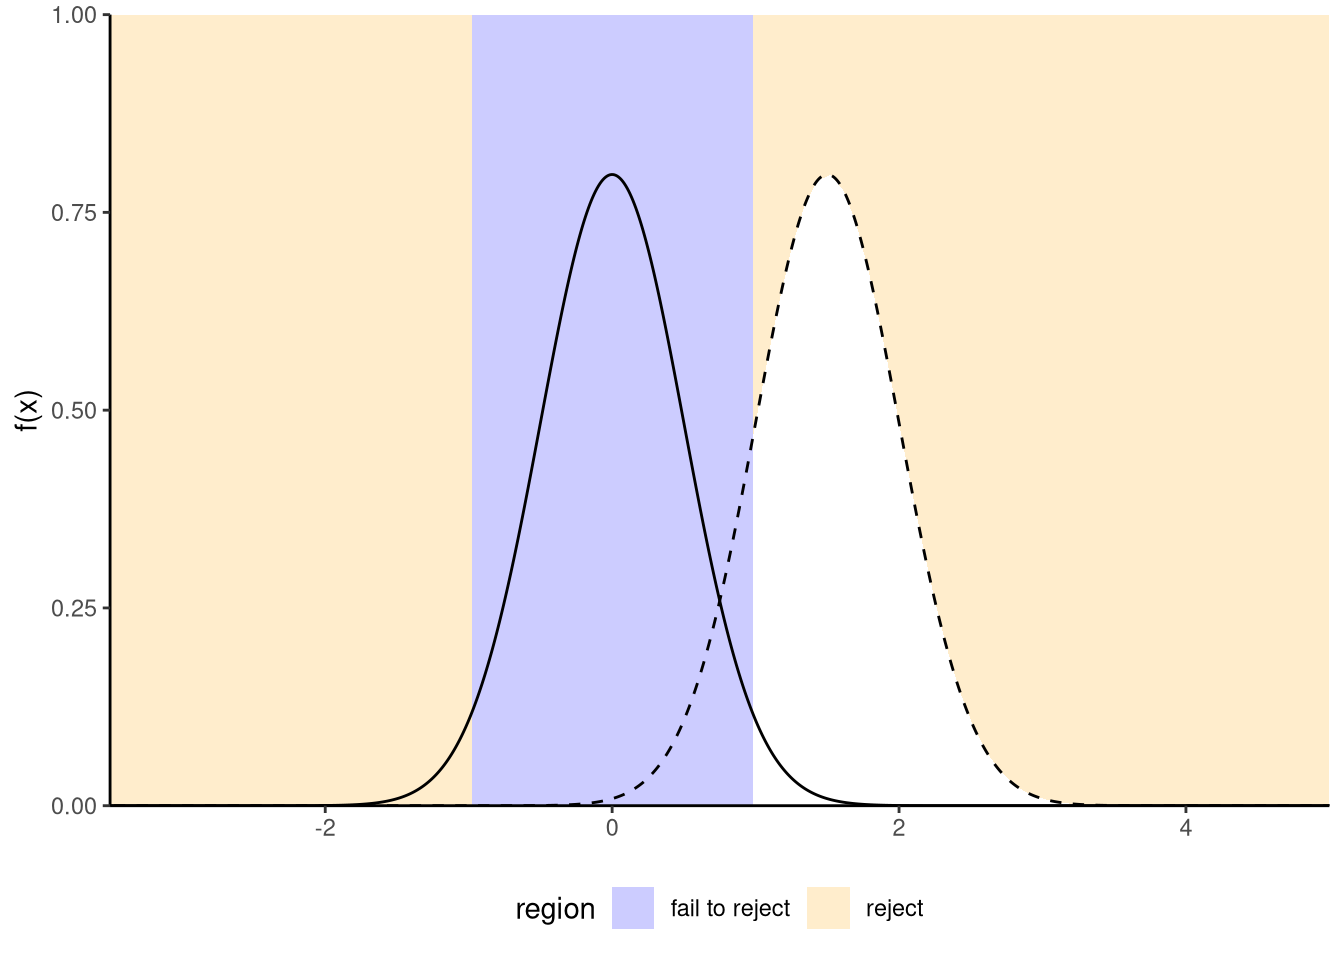
\includegraphics[width=0.7\linewidth]{MATH60604A_Statistical_modelling_files/figure-latex/power3-1} 

}

\caption{Increase of power due to an increase in the sample size or a decrease of standard deviation of the population: the null distribution (full line) is more concentrated. Power is given by the area (white) under the curve of the alternative distribution (dashed). In general, the null distribution changes with the sample size.}\label{fig:power3}
\end{figure}

We want a test to have high power, i.e., that \(\gamma\) be as close to 1 as possible. Minimally, the power of the test should be \(\alpha\) because we reject the null hypothesis \(\alpha\) fraction of the time even when \(\mathscr{H}_0\) is true. Power depends on many criteria, notably

\begin{itemize}
\tightlist
\item
  the effect size: the bigger the difference between the postulated value for \(\theta_0\) under \(\mathscr{H}_0\) and the observed behavior, the easier it is to detect it.
  (Figure \ref{fig:power3});
\item
  variability: the less noisy your data, the easier it is to detect differences between the curves (big differences are easier to spot, as Figure \ref{fig:power2} shows);
\item
  the sample size: the more observation, the higher our ability to detect significative differences because the standard error decreases with sample size \(n\) at a rate (typically) of \(n^{-1/2}\). The null distribution also becomes more concentrated as the sample size increase.
\item
  the choice of test statistic: for example, rank-based statistics discard information about the actual values and care only about relative ranking. Resulting tests are less powerful, but are typically more robust to model misspecification and outliers. The statistics we will choose are standard and amongst the most powerful: as such, we won't dwell on this factor.
\end{itemize}

To calculate the power of a test, we need to single out a specific alternative hypothesis. In very special case, analytic derivations are possible: for example, the one-sample \emph{t}-test statistic \(T=\sqrt{n}(\overline{X}_n-\mu_0)/S_n \sim \mathcal{T}_{n-1}\) for a normal sample follows a noncentral Student-\(t\) distribution with noncentrality parameter \(\Delta\) if the expectation of the population is \(\Delta + \mu_0\). In general, such closed-form expressions are not easily obtained and we compute instead the power of a test through Monte Carlo methods. For a given alternative, we simulate repeatedly samples from the model, compute the test statistic on these new samples and the associated \emph{p}-values based on the postulated null hypothesis. We can then calculate the proportion of tests that lead to a rejection of the null hypothesis at level \(\alpha\), namely the percentage of \emph{p}-values smaller than \(\alpha\).

\hypertarget{confidence-interval}{%
\subsection{Confidence interval}\label{confidence-interval}}

A \textbf{confidence interval} is an alternative way to present the conclusions of an hypothesis test performed at significance level \(\alpha\). It is often combined with a point estimator \(\hat{\theta}\) to give an indication of the variability of the estimation procedure. Wald-based \((1-\alpha)\) confidence intervals for a parameter \(\theta\) are of the form
\begin{align*}
\widehat{\theta} \pm \mathfrak{q}_{\alpha/2} \; \mathrm{se}(\widehat{\theta})
\end{align*}
where \(\mathfrak{q}_{\alpha/2}\) is the \(1-\alpha/2\) quantile of the null distribution of the Wald statistic
\begin{align*}
T =\frac{\widehat{\theta}-\theta}{\mathrm{se}(\widehat{\theta})},
\end{align*}
and where \(\theta\) represents the postulated value for the fixed, but unknown value of the parameter. The bounds of the confidence intervals are random variables, since both \(\widehat{\theta}\) and \(\mathrm{se}(\widehat{\theta})\) are random variables: their values depend on the sample, and will vary from one sample to another.

For example, for a random sample \(X_1, \ldots, X_n\) from a normal distribution \(\mathsf{No}(\mu, \sigma)\), the (\(1-\alpha\)) confidence interval for the population mean \(\mu\) is
\begin{align*}
\overline{X} \pm t_{n-1, \alpha/2} \frac{S}{\sqrt{n}}
\end{align*}
where \(t_{n-1,\alpha/2}\) is the \(1-\alpha/2\) quantile of a Student-\(t\) distribution with \(n-1\) degrees of freedom.

Before the interval is calculated, there is a \(1-\alpha\) probability that \(\theta\) is contained in the \textbf{random} interval \((\widehat{\theta} - \mathfrak{q}_{\alpha/2} \; \mathrm{se}(\widehat{\theta}), \widehat{\theta} + \mathfrak{q}_{\alpha/2} \; \mathrm{se}(\widehat{\theta}))\), where \(\widehat{\theta}\) denotes the estimator. Once we obtain a sample and calculate the confidence interval, there is no more notion of probability: the true value of the parameter \(\theta\) is either in the confidence interval or not. We can interpret confidence interval's as follows: if we were to repeat the experiment multiple times, and calculate a \(1-\alpha\) confidence interval each time, then roughly \(1-\alpha\) of the calculated confidence intervals would contain the true value of \(\theta\) in repeated samples (in the same way, if you flip a coin, there is roughly a 50-50 chance of getting heads or tails, but any outcome will be either). Our confidence is in the \emph{procedure} we use to calculate confidence intervals and not in the actual values we obtain from a sample.

\begin{figure}

{\centering 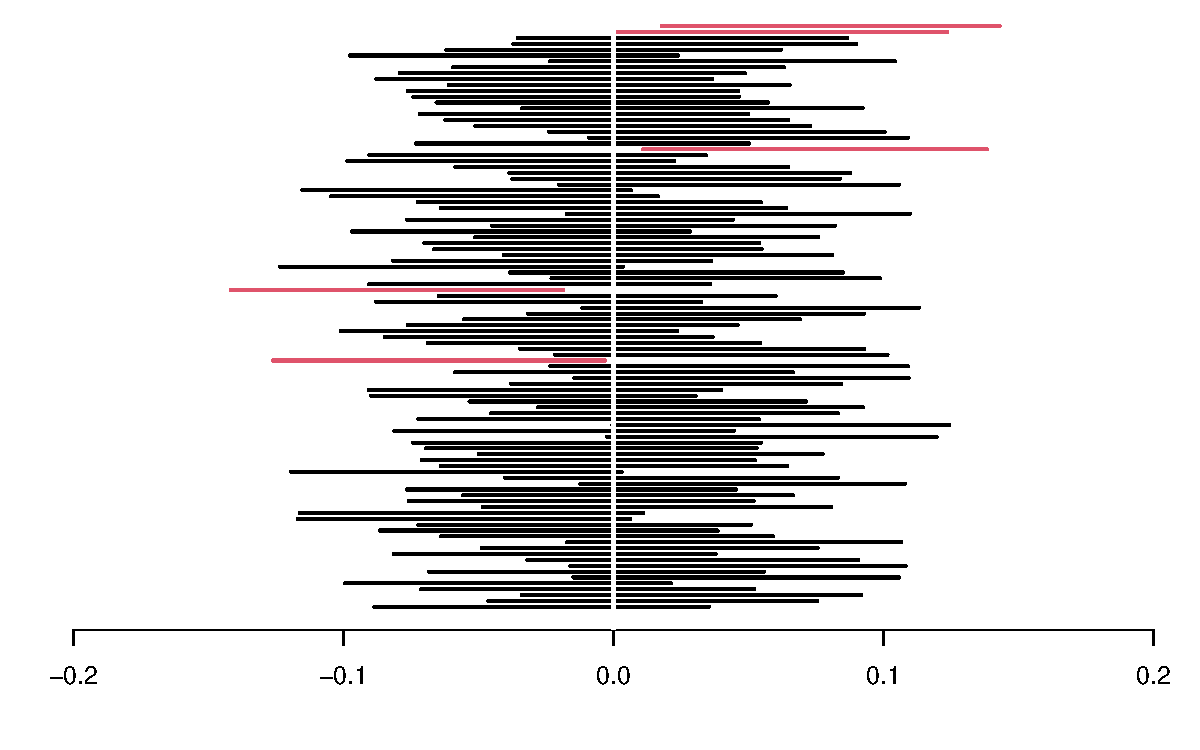
\includegraphics[width=0.7\linewidth]{MATH60604A_Statistical_modelling_files/figure-latex/intconf-1} 

}

\caption{95\% confidence intervals for the mean of a standard normal population $\mathsf{No}(0,1)$, with 100 random samples. On average, 5\% of these intervals fail to include the true mean value of zero (in red).}\label{fig:intconf}
\end{figure}

If we are only interested in the binary decision rule reject/fail to reject \(\mathscr{H}_0\), the confidence interval is equivalent to a \emph{p}-value since it leads to the same conclusion. Whereas the \(1-\alpha\) confidence interval gives the set of all values for which the test statistic doesn't provide enough evidence to reject \(\mathscr{H}_0\) at level \(\alpha\), the \emph{p}-value gives the probability under the null of obtaning a result more extreme than the postulated value and so is more precise for this particular value. If the \emph{p}-value is smaller than \(\alpha\), our null value \(\theta\) will be outside of the confidence interval and vice-versa.

\begin{example}[Online purchases of millenials]
\protect\hypertarget{exm:achats-milleniaux}{}{\label{exm:achats-milleniaux} \iffalse (Online purchases of millenials) \fi{} }
Suppose a researcher studies the evolution of online sales in Canada. She postulates that generation Y members make more online purchase than older generations. A survey is sent to a simple random sample of \(n=500\) individuals from the population with 160 members of generation Y and 340 older people. The response ariable is the total amount of online goods purchased in the previous month (in dollars).
\end{example}

In this example, we consider the difference between the average amount spent by Y members and those of previous generations: the mean difference in the samples is -16.49 dollars and thus millenials spend more. However, this in itself is not enough to conclude that the different is significative, nor can we say it is meaningful. The amount spent online varies from one individual to the next (and plausibly from month to month), and so different random samples would yield different mean differences.

The first step of our analysis is defining the parameters corresponding to quantities of interest and formulating the null and alternative hypothesis as a function of these parameters. We will consider a test for the difference in mean of the two populations, say \(\mu_1\) for the expected amount spent by generation Y and \(\mu_2\) for older generations, with respective standard errors \(\sigma_1\) and \(\sigma_2\). We next write down our hypothesis: the researcher is interested in whether millenials spend more, so this is the alternative hypothesis, \(\mathscr{H}_a: \mu_1 > \mu_2\). The null consists of all other values \(\mathscr{H}_0: \mu_1 \leq \mu_2\), but only \(\mu_1=\mu_2\) matters for the purpose of testing (why?)

The second step is the choice of test statistic. We consider the \citet{Welch:1947} statistic for a difference in mean between two samples,
\begin{align*}
T = \frac{\overline{X}_1 - \overline{X}_2}{\left(\frac{S_1^2}{n_1}+\frac{S_2^2}{n_2} \right)^{1/2}}, \end{align*}
where \(\overline{X}_i\) is the sample mean, \(S_i^2\) is the unbiased variance estimator and \(n_i\) is the sample size for group \(i\) (\(i=1, 2\)). If the mean difference between the two samples is zero, then \(\overline{X}_1-\overline{X}_2\) has mean zero and the difference has variance \(\sigma^2_1/n_1+\sigma^2_2/n_2\). For our sample, the value of statistic is \(T=-2.76\) Since the value changes from one sample to the next, we need to determine if this value is compatible with the null hypothesis by comparing it to the null distribution of \(T\) (when \(\mathscr{H}_0\) is true and \(\mu_1-\mu_2=0\)). We perform the test at level \(\alpha=0.05\).

The third step consists in obtaining a benchmark to determine if our result is extreme or unusual. To make comparisons easier, we standardize the statistic so its has mean zero and variance one under the null hypothesis \(\mu_1=\mu_2\), so as to obtain a dimensionless measure whose behaviour we know for large sample. The (mathematical) derivation of the null distribution is beyond the scope of this course, and will be given in all cases. Asymptotically, \(T\) follows a standard normal distribtion \(\mathsf{No}(0, 1)\), but there exists a better finite-sample approximation when \(n_1\) or \(n_2\) is small; we use \citet{Satterthwaite:1946} and a Student-\(t\) distribution as null distribution.

It only remains to compute the \emph{p}-value. If the null distribution is well-specified and \(\mathscr{H}_0\) is true, then the random variable \(P\) is uniform on \([0, 1]\); we thus expect to obtain under the null something larger than 0.95 only 5\% of the time for our one-sided alternative since we consider under \(\mathscr{H}_0\) the event \(\mathsf{Pr}(T > t)\). The \(p\)-value is \(1\) and, at level 5\%, we reject the null hypothesis to conclude that millenials spend significantly than previous generation for monthly online purchases, with an estimated average difference of -16.49.

\begin{example}[Price of Spanish high speed train tickets]
\protect\hypertarget{exm:price-trains-tests}{}{\label{exm:price-trains-tests} \iffalse (Price of Spanish high speed train tickets) \fi{} }The Spanish national railway company, \href{https://www.renfe.com/}{Renfe}, manages regional and high speed train tickets all over Spain and The Gurus \href{https://www.kaggle.com/thegurusteam/spanish-high-speed-rail-system-ticket-pricing}{harvested} the price of tickets sold by Renfe. We are interested in trips between Madrid and Barcelona and, for now, ask the question: are tickets more expensive one way or another? To answer this, we consider a sample of 10000 tickets, but restrict attention to AVE tickets sold at Promo rate. Our test statistic will again be the mean difference between the price (in euros) for a train ticket for Madrid--Barcelona (\(\mu_1\)) and the price for Barcelona--Madrid (\(\mu_2\)), i.e., \(\mu_1-\mu_2\). The null hypothesis is that there are no difference in price, so \(\mathscr{H}_0: \mu_1-\mu_2=0\). We again use Welch test statistic for two samples.
\end{example}

\begin{Shaded}
\begin{Highlighting}[]
\CommentTok{\# Library for manipulating data, including the pipe operator (\%\textgreater{}\%)}
\KeywordTok{library}\NormalTok{(poorman)}
\CommentTok{\# Load data}
\KeywordTok{data}\NormalTok{(renfe, }\DataTypeTok{package =} \StringTok{"hecstatmod"}\NormalTok{)}
\KeywordTok{head}\NormalTok{(renfe, }\DataTypeTok{n =} \DecValTok{5}\NormalTok{)}
\end{Highlighting}
\end{Shaded}

\begin{verbatim}
## # A tibble: 5 x 7
##   price type    class      fare     dest             duration wday 
##   <dbl> <fct>   <fct>      <fct>    <fct>               <dbl> <fct>
## 1 143.  AVE     Preferente Promo    Barcelona-Madrid      190 6    
## 2 182.  AVE     Preferente Flexible Barcelona-Madrid      190 2    
## 3  86.8 AVE     Preferente Promo    Barcelona-Madrid      165 7    
## 4  86.8 AVE     Preferente Promo    Barcelona-Madrid      190 7    
## 5  69.0 AVE-TGV Preferente Promo    Barcelona-Madrid      175 4
\end{verbatim}

\begin{Shaded}
\begin{Highlighting}[]
\CommentTok{\# Sub{-}sample with only Promo tickets}
\NormalTok{renfe\_promo \textless{}{-}}\StringTok{ }\NormalTok{renfe }\OperatorTok{\%\textgreater{}\%}\StringTok{ }\KeywordTok{subset}\NormalTok{(fare }\OperatorTok{==}\StringTok{ "Promo"}\NormalTok{)}
\CommentTok{\# two{-}sample t{-}test and mean difference}
\NormalTok{ttest \textless{}{-}}\StringTok{ }\KeywordTok{t.test}\NormalTok{(price}\OperatorTok{\textasciitilde{}}\NormalTok{dest, }\DataTypeTok{data =}\NormalTok{ renfe\_promo)}
\NormalTok{ttest }\CommentTok{\#print result}
\end{Highlighting}
\end{Shaded}

\begin{verbatim}
## 
## 	Welch Two Sample t-test
## 
## data:  price by dest
## t = -1, df = 8040, p-value = 0.2
## alternative hypothesis: true difference in means is not equal to 0
## 95 percent confidence interval:
##  -1.100  0.209
## sample estimates:
## mean in group Barcelona-Madrid mean in group Madrid-Barcelona 
##                           82.1                           82.6
\end{verbatim}

Rather than use the asymptotic distribution, whose validity stems from the central limit theorem, we could consider another approximation under the less restrictive assumption that the data are exchangeable: under the null hypothesis, there is no difference between the two destinations and so the label for destination (a binary indicator) is arbitrary. The reasoning underlying \href{https://www.jwilber.me/permutationtest/}{permutation tests} is as follows: to create a benchmark, we will consider observations with the same number in each group, but permuting the labels. We then compute the test statistic on each of these datasets. If there are only a handful in each group (fewer than 10), we could list all possible permutations of the data, but otherwise we can repeat this procedure many times, say 9999, to get a good approximation. This gives an approximate distribution from which we can extract the \emph{p}-value by computing the rank of our statistic relative to the others.

\begin{Shaded}
\begin{Highlighting}[]
\CommentTok{\# p{-}value (permutation test)}
\NormalTok{n \textless{}{-}}\StringTok{ }\KeywordTok{nrow}\NormalTok{(renfe\_promo)}
\NormalTok{B \textless{}{-}}\StringTok{ }\FloatTok{1e4}
\NormalTok{ttest\_stats \textless{}{-}}\StringTok{ }\KeywordTok{numeric}\NormalTok{(B) }
\NormalTok{ttest\_stats[}\DecValTok{1}\NormalTok{] \textless{}{-}}\StringTok{ }\NormalTok{ttest}\OperatorTok{$}\NormalTok{statistic}
\KeywordTok{set.seed}\NormalTok{(}\DecValTok{20200608}\NormalTok{) }\CommentTok{\# set seed of pseudo{-}random number generator}
\ControlFlowTok{for}\NormalTok{(i }\ControlFlowTok{in} \DecValTok{2}\OperatorTok{:}\NormalTok{B)\{}
  \CommentTok{\# Recalculate the test statistic, permuting the labels}
\NormalTok{  ttest\_stats[i] \textless{}{-}}\StringTok{ }\KeywordTok{t.test}\NormalTok{(price }\OperatorTok{\textasciitilde{}}\StringTok{ }\NormalTok{dest[}\KeywordTok{sample.int}\NormalTok{(}\DataTypeTok{n =}\NormalTok{ n)], }
                           \DataTypeTok{data =}\NormalTok{ renfe\_promo)}\OperatorTok{$}\NormalTok{statistic}
\NormalTok{\}}
\CommentTok{\# Graphics library}
\KeywordTok{library}\NormalTok{(ggplot2)}
\CommentTok{\# Plot the empirical permutation distribution}
\KeywordTok{ggplot}\NormalTok{(}\DataTypeTok{data =} \KeywordTok{data.frame}\NormalTok{(}\DataTypeTok{statistic =}\NormalTok{ ttest\_stats), }
       \KeywordTok{aes}\NormalTok{(}\DataTypeTok{x=}\NormalTok{statistic)) }\OperatorTok{+}
\StringTok{  }\KeywordTok{geom\_histogram}\NormalTok{(}\DataTypeTok{bins =} \DecValTok{30}\NormalTok{, }\KeywordTok{aes}\NormalTok{(}\DataTypeTok{y=}\NormalTok{..density..), }\DataTypeTok{alpha =} \FloatTok{0.2}\NormalTok{) }\OperatorTok{+}\StringTok{ }
\StringTok{  }\KeywordTok{geom\_density}\NormalTok{() }\OperatorTok{+}\StringTok{ }
\StringTok{  }\KeywordTok{geom\_vline}\NormalTok{(}\DataTypeTok{xintercept =}\NormalTok{ ttest\_stats[}\DecValTok{1}\NormalTok{]) }\OperatorTok{+}\StringTok{ }
\StringTok{  }\KeywordTok{ylab}\NormalTok{(}\StringTok{"density"}\NormalTok{) }\OperatorTok{+}\StringTok{ }
\StringTok{  }\KeywordTok{stat\_function}\NormalTok{(}\DataTypeTok{fun =}\NormalTok{ dnorm, }\DataTypeTok{col =} \StringTok{"blue"}\NormalTok{)}
\end{Highlighting}
\end{Shaded}

\begin{figure}

{\centering 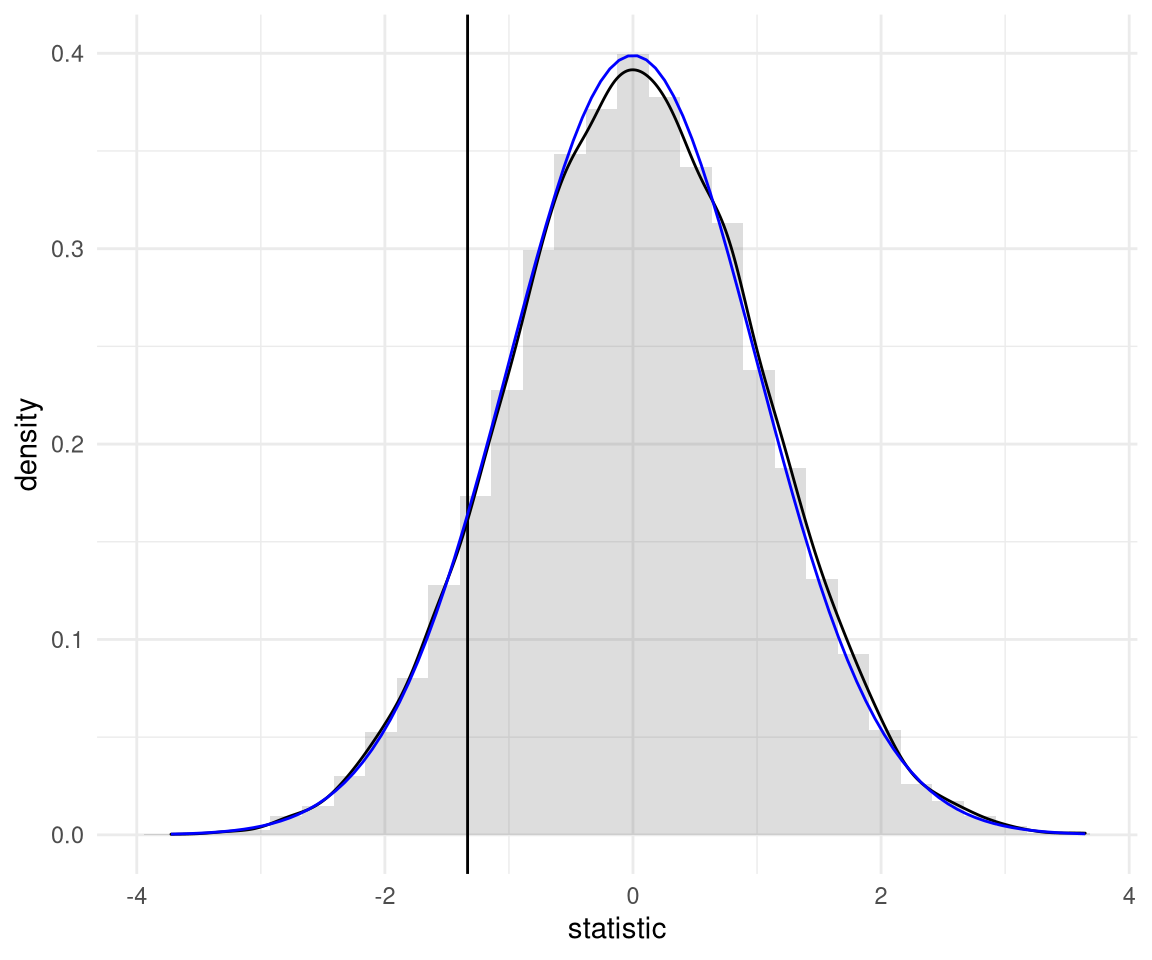
\includegraphics[width=0.7\linewidth]{MATH60604A_Statistical_modelling_files/figure-latex/renfepermut-1} 

}

\caption{Permutation-based approximation to the null distribution of Welch two-sample t-test statistic (histogram and black curve) with standard normal approximation (blue curve) for the price of AVE tickets at promotional rate between Madrid and Barcelona. The value of the test statistic calculated using the original sample is represented by a vertical line.}\label{fig:renfepermut}
\end{figure}

The so-called bootstrap approximation to the \emph{p}-value of the permutation test, \(0.186\), is the proportion of statistics that are more extreme than the one based on the original sample. It is nearly identical to that obtained from the Satterthwaite approximation, \(0.182\) (the Student-\(t\) distribution is numerically equivalent to a standard normal with that many degrees of freedom), as shown in Figure \ref{fig:renfepermut}. Even if our sample is very large (\(n=8059\) observations), the difference is not statistically significative. With a bigger sample (the database has more than 2 million tickets), we could estimate more precisely the average difference, up to 1/100 of an euro: the price difference would eventually become statistically significative, but this says nothing about practical difference: \(0.28\) euros relative to an Promo ticket priced on average \(82.56\) euros is a negligible amount.

\hypertarget{eda}{%
\section{Exploratory Data Analysis}\label{eda}}

Before fitting a model, it is advisable to understand the structure of the data to avoid interpretation errors. Basic knowledge of graphs is required and we will spend some time \href{https://rstudio.cloud/learn/primers/1.1}{addressing this}. Further references include

\begin{itemize}
\tightlist
\item
  \href{https://r4ds.had.co.nz/exploratory-data-analysis.html}{Chapter 3, \emph{\textbf{R} for Data Science} by Garrett Grolemund and Hadley Wickham}
\item
  \href{https://www.openintro.org/book/isrs/}{Section 1.6 of OpenIntro \emph{Introductory Statistics with Randomization and Simulation}}
\item
  \href{https://clauswilke.com/dataviz/}{\emph{Fundamentals of Data Visualization} by Claus O. Wilke}
\item
  \href{https://socviz.co/lookatdata.html\#lookatdata}{Chapter 1 of \emph{Data Visualization: A practical introduction} by Kieran Healy}
\end{itemize}

If exploratory data analysis is often neglected in statistics (perhaps because it has little to no mathematical foundations), it is crucial. More than a rigorous approach, it is an art: Grolemund and Wickham talk of ``state of mind''. The purpose of graphical exploratory data analysis is the extraction of useful information, often through a series of preliminary questions that are refined as the analysis progresses. Of particular interest and the relations and interactions between difference variables and the distribution of the variables themselves. The major steps for undertaking an exploratory analysis are:

\begin{enumerate}
\def\labelenumi{\arabic{enumi}.}
\tightlist
\item
  Formulate questions about the data
\item
  Look for answers using frequency table, descriptive statistics and graphics.
\item
  Refine the questions in light of the finding
\end{enumerate}

In a report, you should highlight the most import features in a summary so that the reader can grasp your understanding and so that you guide him or her in the interpretation of the data.

\hypertarget{polish-your-work}{%
\subsection{Polish your work}\label{polish-your-work}}

Pay as much attention to figures and tables than to the main text. These should always include a legend that describes and summarize the findings in the graph (so that the latter is standalone), name of variables (including units) on the axes, but also proper formatting so that the labels and numbers are readable (good printing quality, not too small). One picture is worth 1000 words, but make sure the graph tells a coherent story and that it is mentioned in the main text. Also ensure that only the necessary information is displayed: superfluous information (spurious digits, useless summary statistics) should not be presented.

\hypertarget{variable-type}{%
\subsection{Variable type}\label{variable-type}}

The data we will handled are stored in tables or frames. If the data frame is stocked in long format, each line corresponds to an observation and each column to a variable: the entries of the data base contain the (numeric) values.

The alternative is wide format, whereby the columns represent categorical variables and the entries are values of the response for a specific category (notably contingency tables). Figure \ref{fig:longvswide} shows the difference between the two structures. Software typically require long formatted database for modelling purposes.

\begin{figure}

{\centering 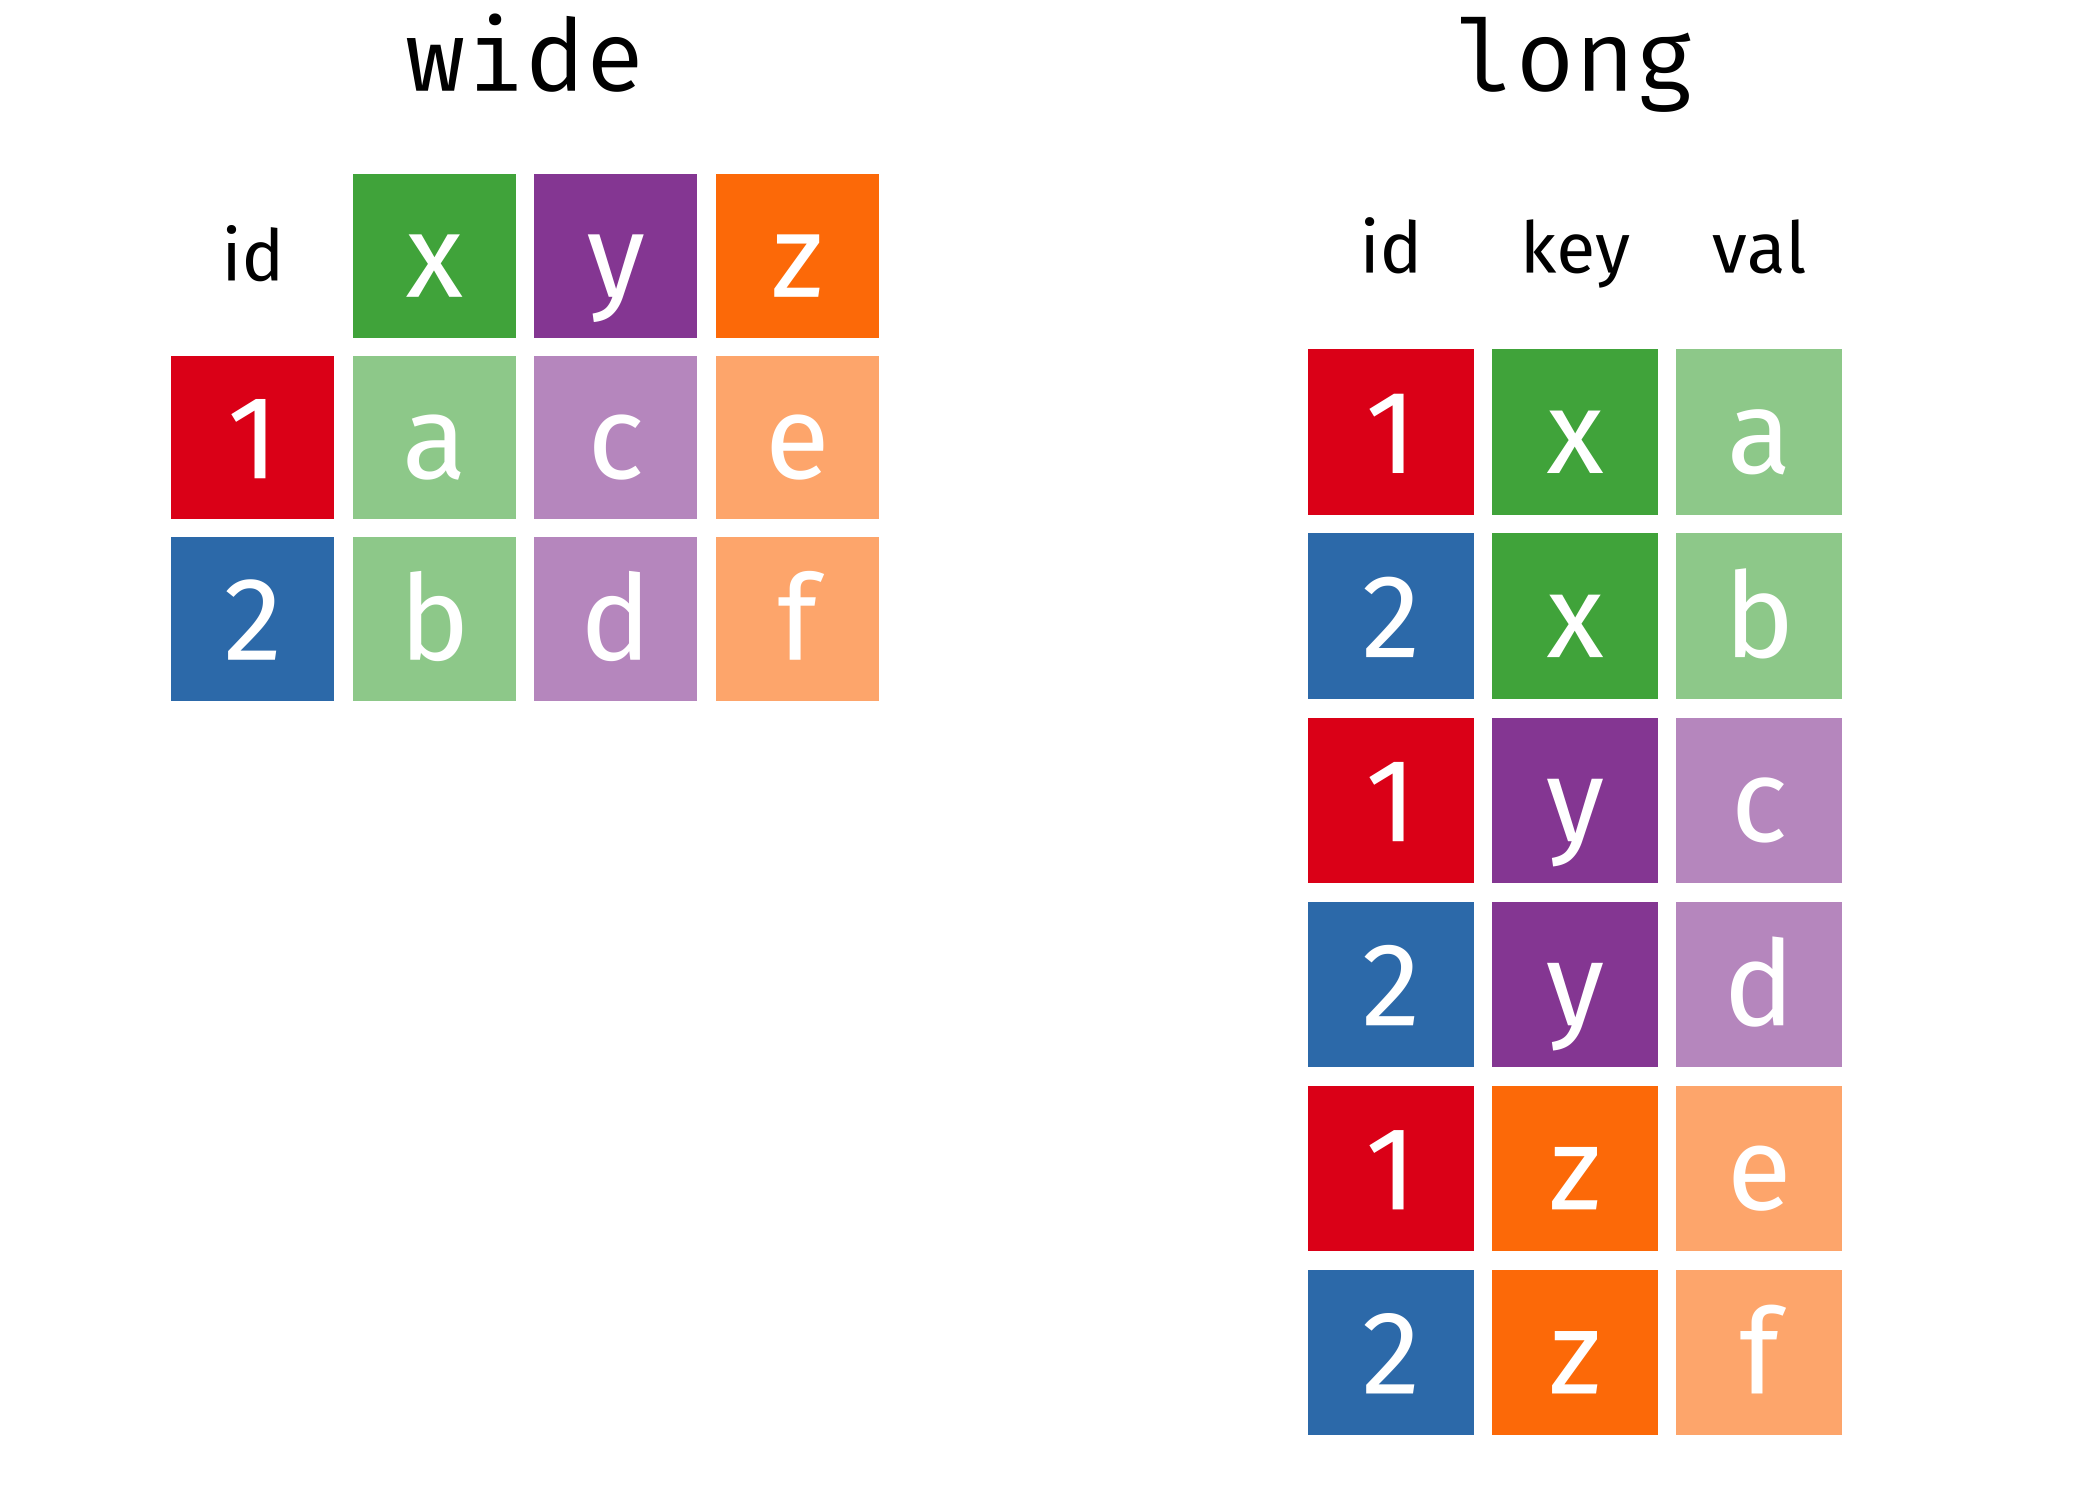
\includegraphics[width=0.7\linewidth]{images/original-dfs-tidy} 

}

\caption{Long versus wide-format for data tables (illustration by Garrick Aden-Buie).}\label{fig:longvswide}
\end{figure}

\begin{itemize}
\tightlist
\item
  a \textbf{variable} represents a characteristic of the population, for example the sex of an individual, the price of an item, etc.
\item
  an \textbf{observation} is a set of measures (variables) collected under identical conditions for an individual or at a given time.
\end{itemize}

The choice of statistical model and test depends on the underlying type of the data collected. There are many choices: quantitative (discrete or continuous) if the variables are numeric, or qualitative (binary, nominal, ordinal) if they can be described using an adjective; I prefer the term categorical, which is more evocative.

Most of the models we will deal with are so-called regression models, in which the mean of a quantitative variable is a function of other variables, termed explanatories. There are two types of numerical variables

\begin{itemize}
\tightlist
\item
  a discrete variable takes a countable number of values, prime examples being binary variables or count variables.
\item
  a continuous variable can take (in theory) an infinite possible number of values, even when measurements are rounded or measured with a limited precision (time, width, mass). In many case, we could also consider discrete variables as continuous if they take enough values (e.g., money).
\end{itemize}

Categorical variables take only a finite of values. They are regrouped in two groups, nominal if there is no ordering between levels (sex, color, country of origin) or ordinal if they are ordered (Likert scale, salary scale) and this ordering should be reflected in graphs or tables. We will bundle every categorical variable using arbitrary encoding for the levels: for modelling, these variables taking \(K\) possible values (or levels) must be transformed into a set of \(K-1\) binary 0/1 variables, the omitted level corresponding to a baseline. Failing to declare categorical variables in your favorite software is a common mistake, especially when these are saved in the database using integers rather than strings.

\hypertarget{graphs}{%
\subsection{Graphs}\label{graphs}}

The main type of graph for representing categorical variables is bar plot (and modifications thereof). In a bar plot, the frequency of each category is represented in the \(y\)-axis as a function of the (ordered) levels on the \(x\)-axis. This representation is superior to the \href{http://www.perceptualedge.com/articles/08-21-07.pdf}{ignominious pie chart}, a nuisance that ought to be banned (humans are very bad at comparing areas and a simple rotation changes the perception of the graph)!

\begin{figure}

{\centering 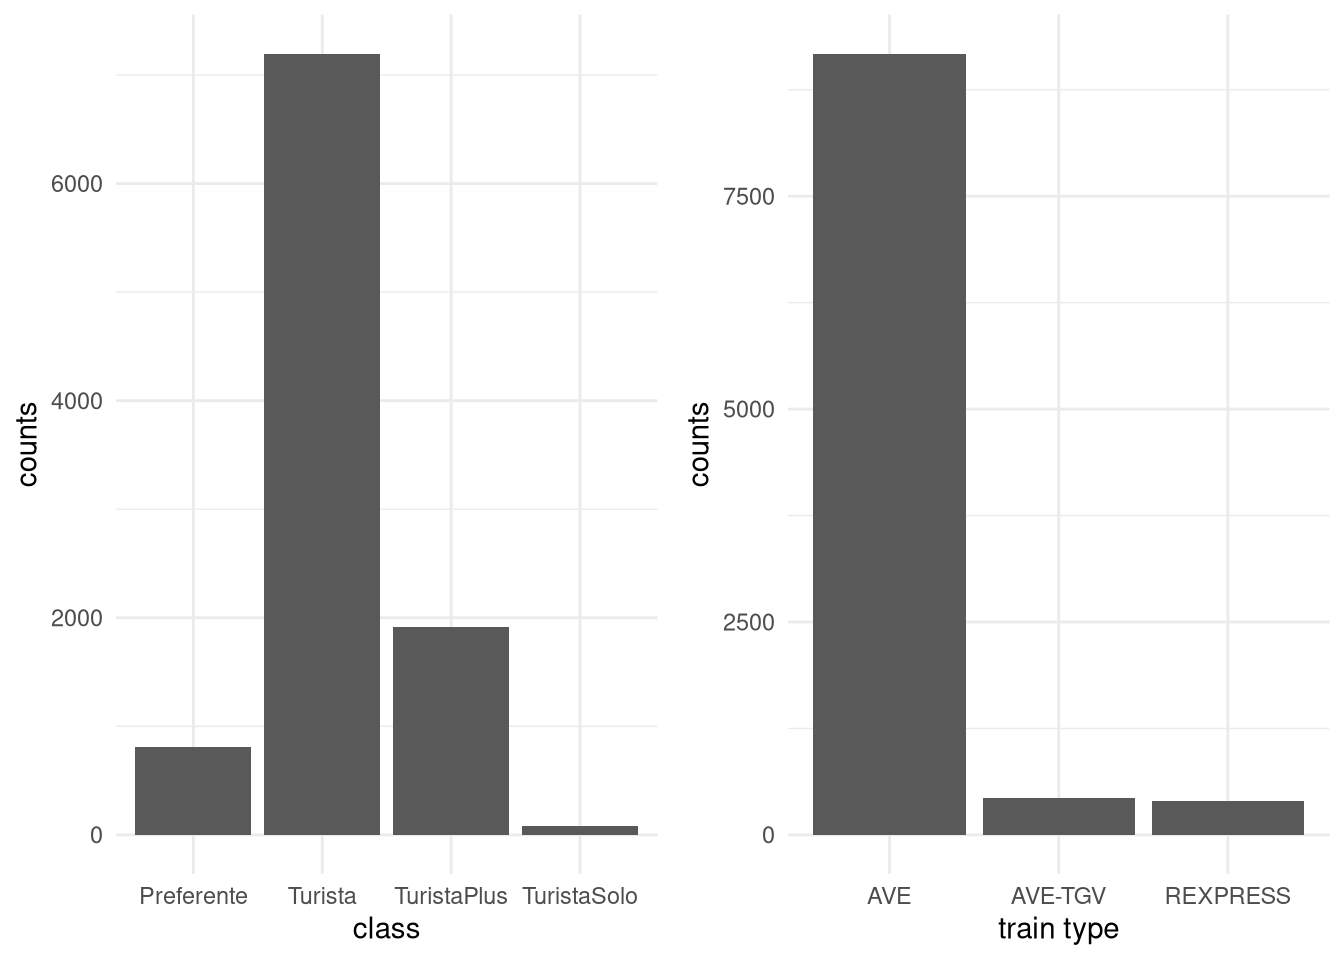
\includegraphics[width=0.7\linewidth]{MATH60604A_Statistical_modelling_files/figure-latex/barplotrenfe-1} 

}

\caption{Bar plot of ticket class for Renfe tickets data}\label{fig:barplotrenfe}
\end{figure}

Continuous variables can take as many distinct values as there are observations, so we cannot simply count the number of occurences by unique values. Instead, we bin them into distinct intervals so as to obtain an histogram. The number of class depends on the number of observations: as a rule of thumb, the number of bins should not exceed \(\sqrt{n}\), where \(n\) is the sample size. We can then obtain the frequency in each class, or else normalize the histogram so that the area under the bands equals one: this yields a discrete approximation of the underlying density function. Varying the number of bins can help us detect patterns (rounding, asymmetry, multimodality).

Since we bin observations together, it is sometimes difficult to see where they fall. Adding rugs below or above the histogram will add observation about the range and values taken, where the heights of the bars in the histogram carry information about the (relative) frequency of the intervals.

\begin{figure}

{\centering 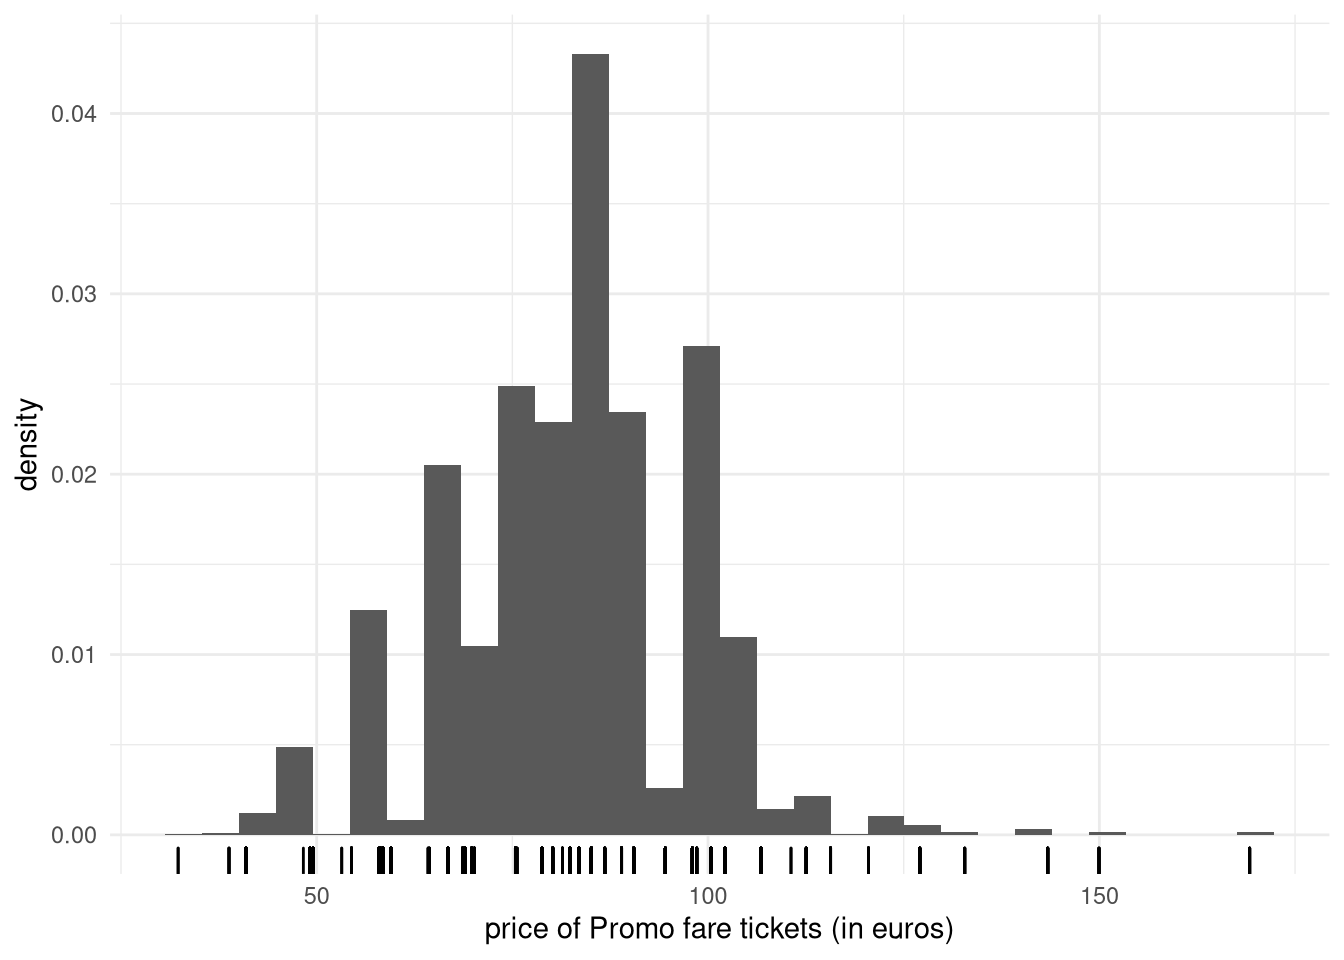
\includegraphics[width=0.7\linewidth]{MATH60604A_Statistical_modelling_files/figure-latex/histrenfe-1} 

}

\caption{Histogram of Promo tickets for Renfe ticket data}\label{fig:histrenfe}
\end{figure}

If we have a lot of data, it sometimes help to focus only on selected summary statistics. A box-and-whiskers plot (or boxplot) represents five numbers

\begin{itemize}
\tightlist
\item
  The box gives the quartiles \(q_1, q_2, q_3\) of the distribution. The middle bar \(q_2\) is thus the median, so 50\% of the observations are smaller or larger than this number.
\item
  The length of the whiskers is up to \(1.5\) times the interquartiles range \(q_3-q_1\) (the whiskers extend until the latest point in the interval, so the largest observation that is smaller than \(q_3+1.5(q_3-q_1)\), etc.)
\item
  Observations beyond the whiskers are represented by dots or circles, sometimes termed outliers. However, beware of this terminology: the larger the sample size, the more values will fall outside the whiskers. This is a drawback of boxplots, which was conceived at a time where the size of data sets was much smaller than what is current standards.
\end{itemize}

\begin{figure}

{\centering 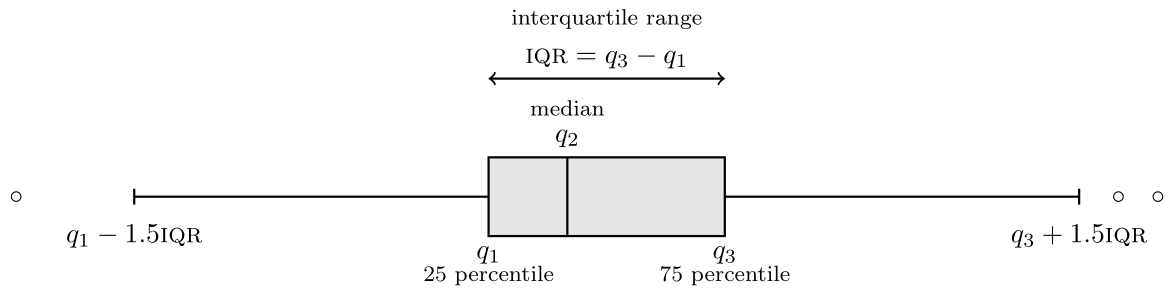
\includegraphics[width=0.7\linewidth]{images/01-intro-boxplot} 

}

\caption{Box-and-whiskers plot}\label{fig:boxplot}
\end{figure}

We can represent the distribution of a response variable as a function of a categorical variable by drawing a boxplot for each category and laying them side by side. A third variable, categorical, can be added via a color palette, as shown in Figure \ref{fig:histboxplot}.

\begin{figure}

{\centering 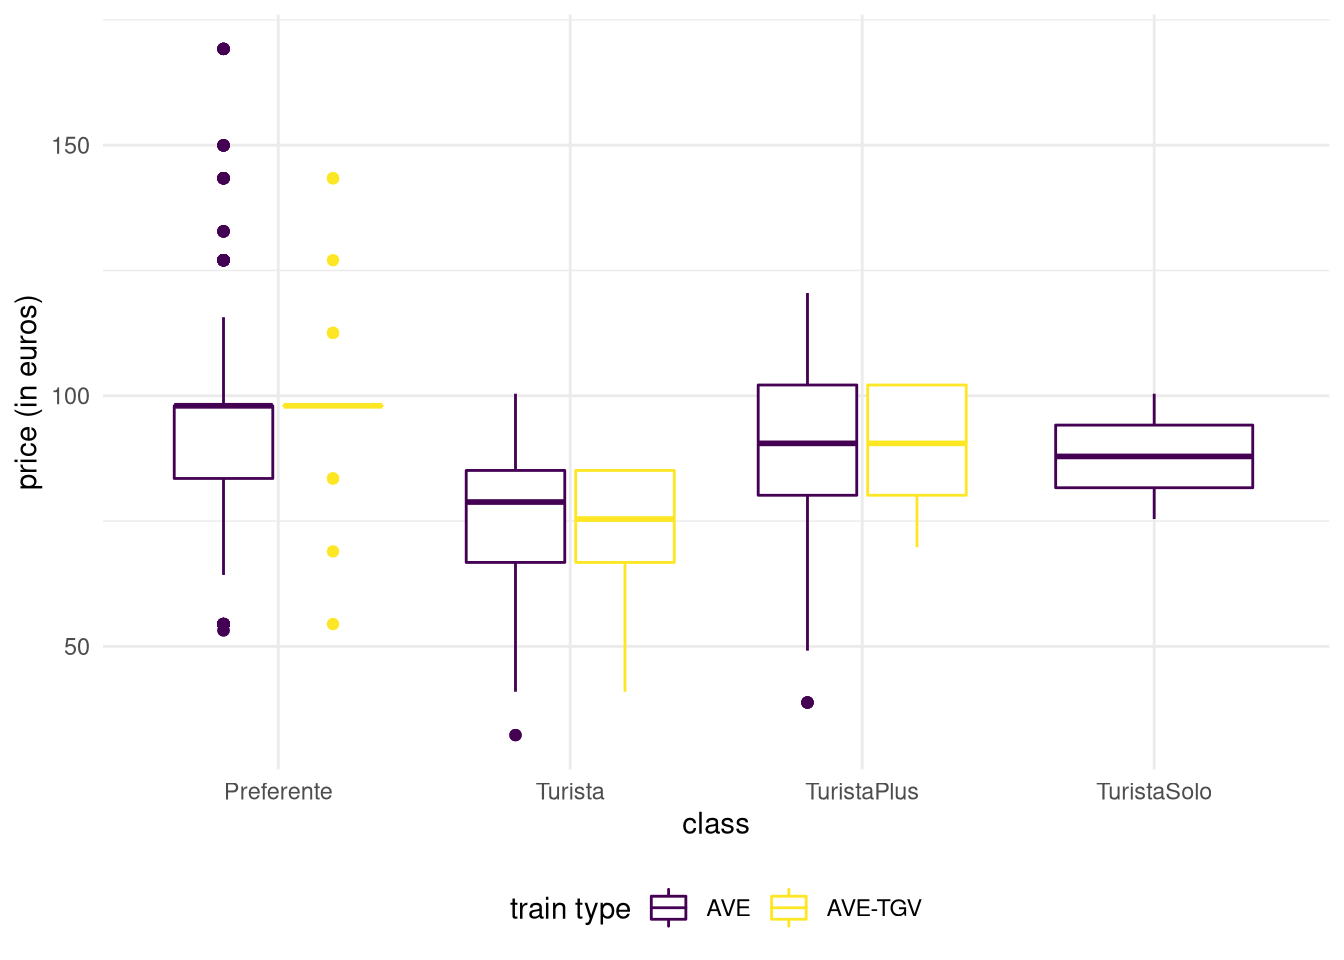
\includegraphics[width=0.7\linewidth]{MATH60604A_Statistical_modelling_files/figure-latex/histboxplot-1} 

}

\caption{Box-and-whiskers plots for Promo fare tickets as a function of class and type for the Renfe tickets data.}\label{fig:histboxplot}
\end{figure}

Scatterplots are used to represent graphically the co-variation between two continuous variables: each tuple gives the coordinate of the point. If only a handful of large values are visible on the graph, a transformation may be useful: oftentimes, you will encounter graphs where the \(x\)- or \(y\)-axis is on the log-scale when the underlying variable is positive. If the number of data points is too large, it is hard to distinguish points because they are overlaid: adding transparency, or binning using a two-dimensional histogram with the frequency represented using color are potential solutions. The left panel of Figure \ref{fig:scatterplot} shows the 100 simulated observations, whereas the right-panel shows a larger sample of 10 000 points using hexagonal binning, an analog of the bivariate density.

\begin{figure}

{\centering 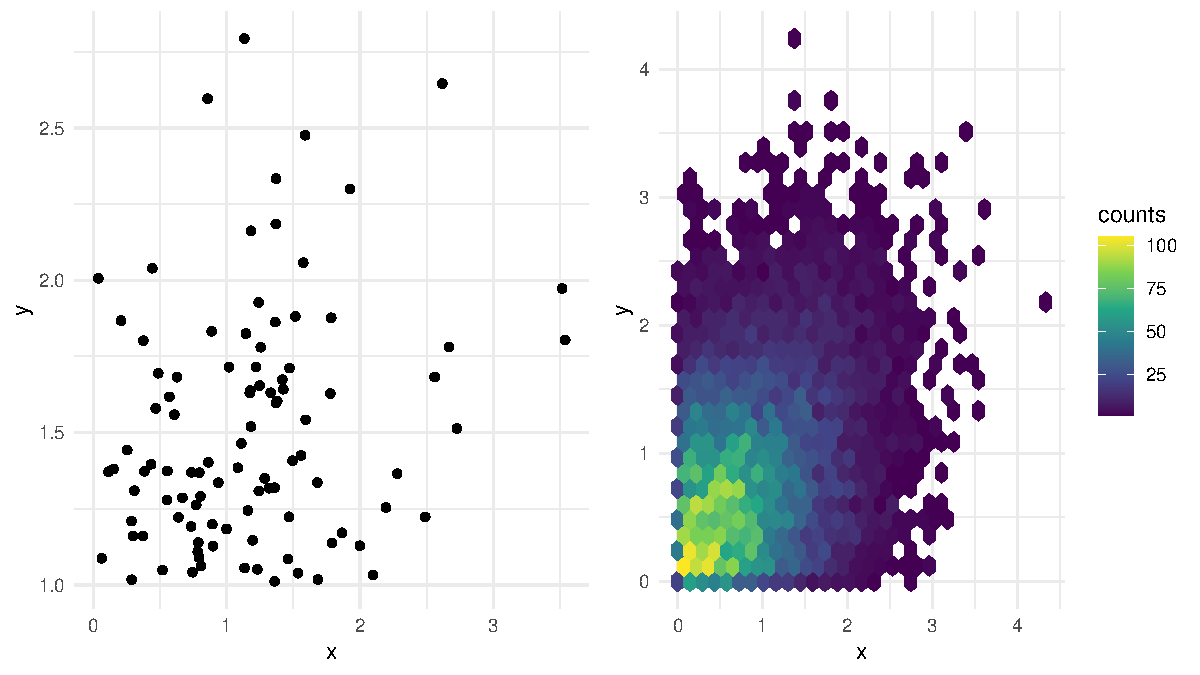
\includegraphics[width=0.7\linewidth]{MATH60604A_Statistical_modelling_files/figure-latex/scatterplot-1} 

}

\caption{Scatterplot (left) and hexagonal heatmap of bidimensional bin counts (right) of simulated data.}\label{fig:scatterplot}
\end{figure}

Sometimes, continuous data have a particular structure, mostly when observations are collected over space or time. Time series are ordered and the response should be plotted on the \(y\)-axis as a function of time (on the \(x\)-axis). It is customary to draw segments between observations, but this display is sometimes misleading.

\begin{figure}

{\centering 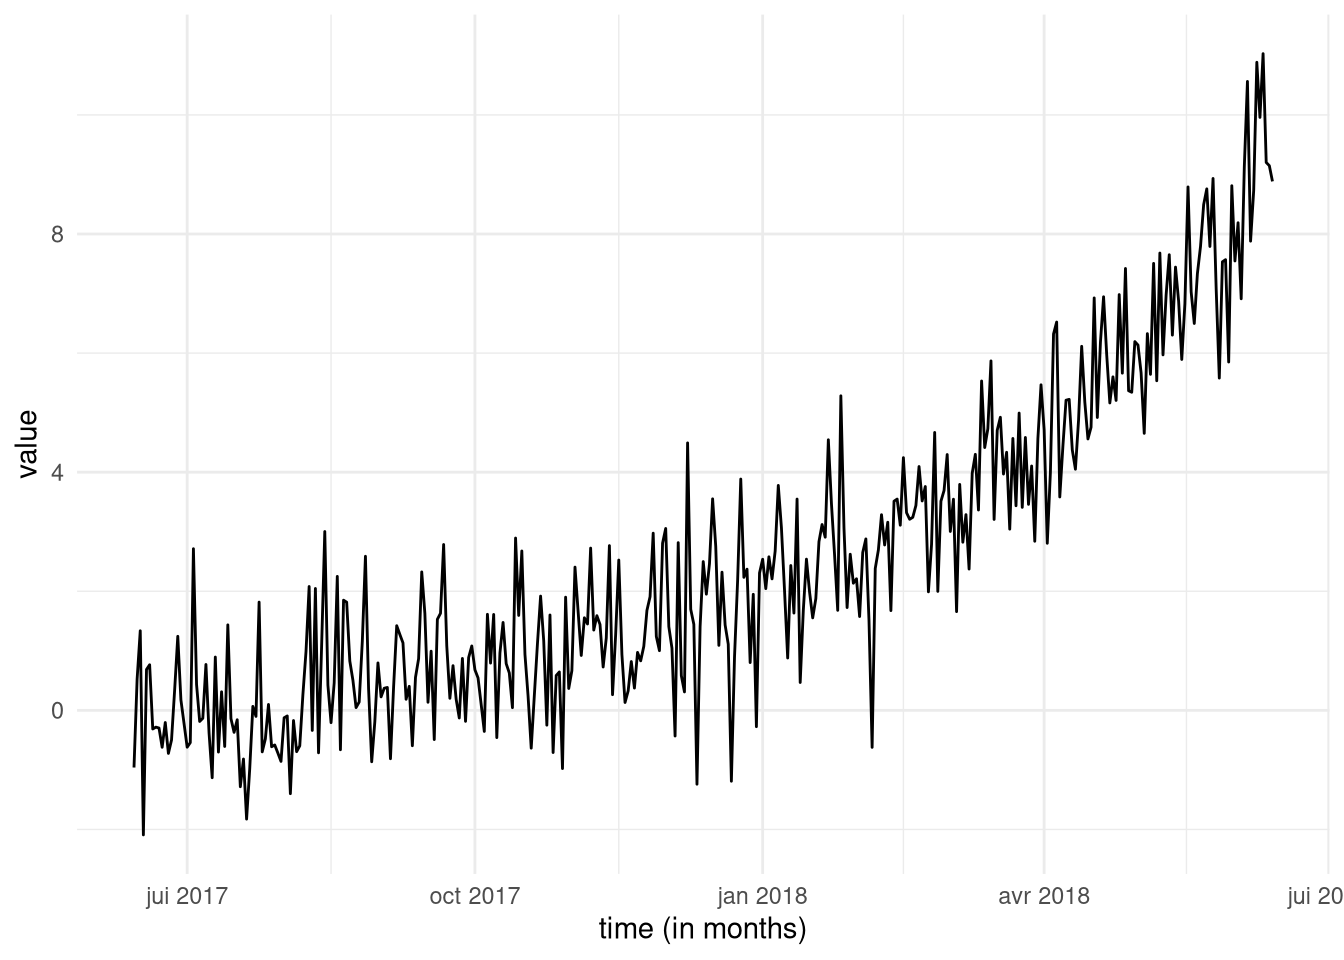
\includegraphics[width=0.7\linewidth]{MATH60604A_Statistical_modelling_files/figure-latex/seriechrono-1} 

}

\caption{Graphical representation of a time series.}\label{fig:seriechrono}
\end{figure}

\hypertarget{exploratory-data-analysis}{%
\subsection{Exploratory data analysis}\label{exploratory-data-analysis}}

Rather than describe in details the exploratory analysis procedure, we proceed with an example that illustrates the process on the Renfe ticket dataset that was introduced previously.

\begin{example}[Exploratory data analysis of Renfe tickets]
\protect\hypertarget{exm:renfe-aed}{}{\label{exm:renfe-aed} \iffalse (Exploratory data analysis of Renfe tickets) \fi{} }First, read the documentation accompanying the dataset! The data base \texttt{renfe} contains the following variables:
\end{example}

\begin{itemize}
\tightlist
\item
  \texttt{price} price of the ticket (in euros);
\item
  \texttt{dest} binary variable indicating the journey, either Barcelona to Madrid (\texttt{0}) or Madrid to Barcelona (\texttt{1});
\item
  \texttt{fare} categorical variable indicating the ticket fare, one of \texttt{AdultoIda}, \texttt{Promo} or \texttt{Flexible};
\item
  \texttt{class} categorical variable giving the ticket class, either \texttt{Preferente}, \texttt{Turista}, \texttt{TuristaPlus} or \texttt{TuristaSolo};
\item
  \texttt{type} categorical variable indicating the type of train, either Alta Velocidad Española (\texttt{AVE}), Alta Velocidad Española jointly with TGV (parternship between SNCF and Renfe for trains to/from Toulouse) \texttt{AVE-TGV} or regional train \texttt{REXPRESS}; only trains labelled \texttt{AVE} or \texttt{AVE-TGV} are high-speed trains.
\item
  \texttt{duration} length of train journey (in minutes);
\item
  \texttt{wday} categorical variable (integer) denoting the week day, ranging from Sunday (\texttt{1}) to Saturday (\texttt{7}).
\end{itemize}

There are no missing values and a quick view of the first row of the data frame (\texttt{head(renfe)}) shows that the data are stored in long format, meaning each line corresponds to a different ticket.
We will begin our exploratory analysis with vague questions, for example

\begin{enumerate}
\def\labelenumi{\arabic{enumi}.}
\tightlist
\item
  What are the factors determining the price and travel time?
\item
  Does travel time depend on the type of train?
\item
  What are the distinctive features of train types?
\item
  What are the main differences between fares?
\end{enumerate}

Except for \texttt{price} and \texttt{duration}, all the other (explanatory) variables are categoricals. These need to be cast into factors (\texttt{factor}), especially integer-valued levels such as \texttt{wday}.

The database is clean and this preliminary preprocessing step has been done already. We can check the type of encoding using the command \texttt{str}, which also shows the data; the function \texttt{summary} is used to obtain descriptive statistics (min, max, mean, quartiles for continuous variables or else frequency for categorical variables); the function also returns the number of missing values (\texttt{NA}) of each column.

Data manipulation is often messy and \textbf{R} base syntax is particularly inelegant: data frames are list whose elements are accessed using \texttt{\$}: for example \texttt{renfe\$price}. A more legible and modular alternative is the pipe operator (\texttt{\%\textgreater{}\%}), with which one creates a logical chain of command (this function is not part of \textbf{R} base packages, but the libraries \texttt{tidyverse} and the minimal alternative \texttt{poorman} include it).

\begin{Shaded}
\begin{Highlighting}[]
\NormalTok{renfe }\OperatorTok{\%\textgreater{}\%}\StringTok{ }\KeywordTok{count}\NormalTok{(class)}
\end{Highlighting}
\end{Shaded}

\begin{verbatim}
##         class    n
## 1  Preferente  809
## 2     Turista 7197
## 3 TuristaPlus 1916
## 4 TuristaSolo   78
\end{verbatim}

\begin{Shaded}
\begin{Highlighting}[]
\CommentTok{\# \textasciigrave{}count\textasciigrave{} is a shortcut for the following syntax}
\NormalTok{renfe }\OperatorTok{\%\textgreater{}\%}\StringTok{ }\KeywordTok{group\_by}\NormalTok{(type) }\OperatorTok{\%\textgreater{}\%}\StringTok{ }\KeywordTok{tally}\NormalTok{()}
\end{Highlighting}
\end{Shaded}

\begin{verbatim}
##       type    n
## 1      AVE 9174
## 2  AVE-TGV  429
## 3 REXPRESS  397
\end{verbatim}

\begin{Shaded}
\begin{Highlighting}[]
\NormalTok{renfe }\OperatorTok{\%\textgreater{}\%}\StringTok{ }\KeywordTok{group\_by}\NormalTok{(fare) }\OperatorTok{\%\textgreater{}\%}\StringTok{ }\KeywordTok{tally}\NormalTok{()}
\end{Highlighting}
\end{Shaded}

\begin{verbatim}
##        fare    n
## 1 AdultoIda  397
## 2  Flexible 1544
## 3     Promo 8059
\end{verbatim}

By counting the number of train tickets in each category, we notice there are as many \texttt{REXPRESS} tickets as there are tickets sold at \texttt{AdultoIda} fare. Using a contingency table to get the number in respective sub-categories of each of those variables confirms that all tickets in the database for RegioExpress trains are sold with the \texttt{AdultoIda} fare and that there is only a single class, \texttt{Turista}. There are few such tickets, only 397 out of 10 000. This raises a new question: why are such trains so unpopular?

\begin{verbatim}
##        fare     type    n
## 1 AdultoIda REXPRESS  397
## 2  Flexible      AVE 1446
## 3  Flexible  AVE-TGV   98
## 4     Promo      AVE 7728
## 5     Promo  AVE-TGV  331
\end{verbatim}

We have only scratched the surface, but one could also notice that there are only 17 duration values on tickets (\texttt{renfe\ \%\textgreater{}\%\ distinct(duration)} or \texttt{unique(renfe\$duration)}). This leads us to think the duration on the ticket (in minutes) is the expected travel time. The majority of those travel time (15 out of 17) are smaller than 3h15, but the other two exceed 9h! Looking at Google Maps, Madrid and Barcelona are 615km apart by car, 500km as the crow flies. this means some trains travel at about 200km/h, while others are closer to 70km/h. What are these slower trains? the variable \texttt{type} is the one most likely to encode this feature, and a quick look shows that the RegioExpress trains fall in the slow category (mystery solved!)

\begin{Shaded}
\begin{Highlighting}[]
\NormalTok{renfe }\OperatorTok{\%\textgreater{}\%}\StringTok{ }
\StringTok{  }\KeywordTok{subset}\NormalTok{(duration }\OperatorTok{\textgreater{}}\StringTok{ }\DecValTok{200}\NormalTok{) }\OperatorTok{\%\textgreater{}\%}\StringTok{ }
\StringTok{  }\KeywordTok{group\_by}\NormalTok{(type, dest) }\OperatorTok{\%\textgreater{}\%}\StringTok{ }
\StringTok{  }\KeywordTok{summarise}\NormalTok{(}\StringTok{"average duration"}\NormalTok{ =}\StringTok{ }\KeywordTok{mean}\NormalTok{(duration), }
            \StringTok{"std. dev"}\NormalTok{ =}\StringTok{ }\KeywordTok{sd}\NormalTok{(duration),}
            \StringTok{"average price"}\NormalTok{ =}\StringTok{ }\KeywordTok{mean}\NormalTok{(price), }
            \StringTok{"std. dev"}\NormalTok{ =}\StringTok{ }\KeywordTok{sd}\NormalTok{(price)) }
\end{Highlighting}
\end{Shaded}

\begin{verbatim}
##       type             dest average duration std. dev average price std. dev
## 1 REXPRESS Barcelona-Madrid              544        0          43.2        0
## 2 REXPRESS Madrid-Barcelona              562        0          43.2        0
\end{verbatim}

The regular trains running between two cities take more than 9h, but one way (Madrid to Barcelona) is 18 minutes slower than in the other direction. More striking, we see that the price of the RegioExpress tickets is fixed: 43.25 euros regardless of direction. This is the most important finding so far, because these are not a sample for price: there is no variability! Graphics could have lead to the discovery (the boxplot of price as a function of train type would collapse to a single value).

\begin{figure}

{\centering 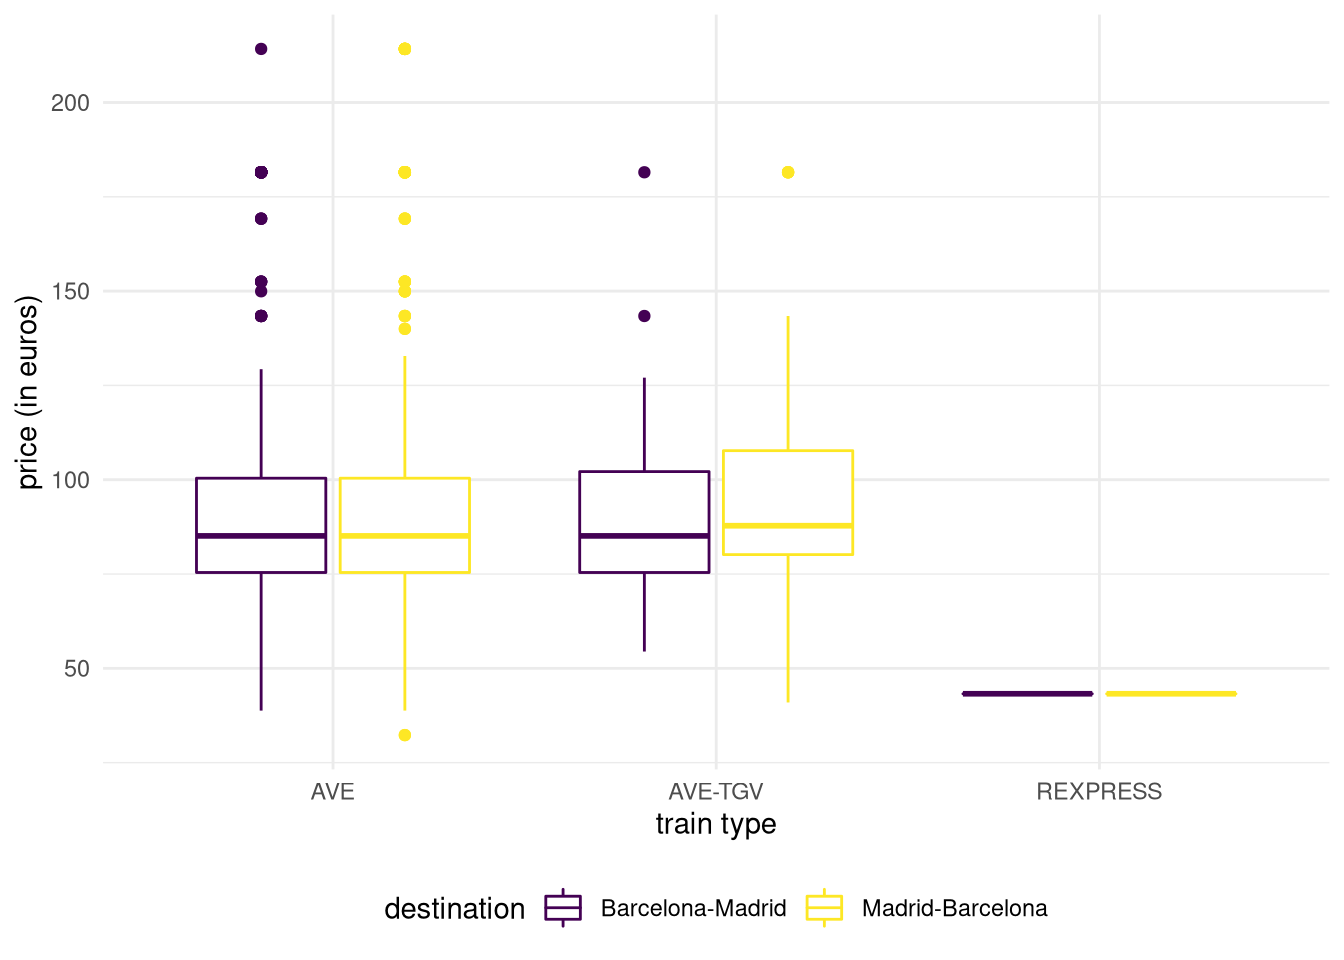
\includegraphics[width=0.7\linewidth]{MATH60604A_Statistical_modelling_files/figure-latex/renfe-aed4-1} 

}

\caption{Boxplot of ticket price as a function of destination and train type.}\label{fig:renfe-aed4}
\end{figure}

We could have suspected that trains labeled \texttt{AVE} are faster: after all, it is the acronym of \emph{Alta Velocidad Española}, literally Spanish high speed. What is the distinction between the two high speed train types. According to the \href{https://www.renfe-sncf.com/rw-en/services/a-unique-experience/Pages/services.aspx}{SNCF website}, AVE-TGV trains are partnership between Renfe and SNCF that operate between France and Spain.

\begin{Shaded}
\begin{Highlighting}[]
\NormalTok{renfe }\OperatorTok{\%\textgreater{}\%}\StringTok{ }
\StringTok{  }\KeywordTok{subset}\NormalTok{(type }\OperatorTok{\%in\%}\StringTok{ }\KeywordTok{c}\NormalTok{(}\StringTok{"AVE"}\NormalTok{,}\StringTok{"AVE{-}TGV"}\NormalTok{)) }\OperatorTok{\%\textgreater{}\%}\StringTok{ }
\StringTok{  }\KeywordTok{group\_by}\NormalTok{(type, dest) }\OperatorTok{\%\textgreater{}\%}\StringTok{ }
\StringTok{  }\KeywordTok{summarise}\NormalTok{(}\StringTok{"average duration"}\NormalTok{ =}\StringTok{ }\KeywordTok{mean}\NormalTok{(duration), }
            \StringTok{"std. dev"}\NormalTok{ =}\StringTok{ }\KeywordTok{sd}\NormalTok{(duration),}
            \StringTok{"average price"}\NormalTok{ =}\StringTok{ }\KeywordTok{mean}\NormalTok{(price),}
            \StringTok{"std. dev"}\NormalTok{ =}\StringTok{ }\KeywordTok{sd}\NormalTok{(price))}
\end{Highlighting}
\end{Shaded}

\begin{verbatim}
##      type             dest average duration std. dev average price std. dev
## 1     AVE Barcelona-Madrid              171     15.9          87.4     19.8
## 2     AVE Madrid-Barcelona              170     16.6          88.2     20.8
## 3 AVE-TGV Barcelona-Madrid              175      0.0          87.0     16.8
## 4 AVE-TGV Madrid-Barcelona              179      0.0          90.6     20.2
\end{verbatim}

The price of high speed trains are on average more than twice as expensive as regular trains. There is strong evidence of heterogeneity (standard deviation of 20 euros), which should raise scrutiny and suggests that high speed train tickets are dynamically priced. There is a single duration time for AVE-TGV tickets. We do not see meaningful differences in price depending on the type or the direction, but fares of ticket class availability may differ depending on whether the train is run in partnership with SNCF.

We have not looked at ticket fare and class, except for RegioExpress trains. Figure \ref{fig:renfe-aed7} shows large disparity in the variance of price according to fare: Promo fare takes many more distinct values than AdultoIda (duh) and Flexible fares. First class tickets (\texttt{Preferente}) are more expensive, but there are fewer observations falling in this group. Turista class is the least expensive for high-speed trains and the most popular. \href{http://web.archive.org/web/20161111134241/http://www.renfe.com/viajeros/tarifas/billete_promo.html}{\texttt{TuristaPlus}} offer an alternative to the latter with more comfort, whereas \texttt{TuristaSolo} gives access to individual seats.

Fare-wise \href{http://web.archive.org/web/20161111134241/http://www.renfe.com/viajeros/tarifas/billete_promo.html}{Promo} and \href{http://web.archive.org/web/20161110220249/http://www.renfe.com/viajeros/tarifas/billete_promoplus.html}{PromoPlus} give access to rebates that can go up to 70\% and 65\%, respectively. Promo tickets cannot be cancelled or exchanged, while both are possible with PromoPlus by paying a penalty amounting to 30-20\% of the ticket price. \href{http://web.archive.org/web/20161108192609/http://www.renfe.com/viajeros/tarifas/billete_flexible.html}{Flexible} fare ticket a sold at the same price as regular high-speed train tickets, but offer additional benefits (and no rebates!)

\begin{Shaded}
\begin{Highlighting}[]
\NormalTok{renfe }\OperatorTok{\%\textgreater{}\%}\StringTok{ }\KeywordTok{subset}\NormalTok{(fare  }\OperatorTok{!=}\StringTok{ "AdultoIda"}\NormalTok{) }\OperatorTok{\%\textgreater{}\%}
\KeywordTok{ggplot}\NormalTok{(}\KeywordTok{aes}\NormalTok{(}\DataTypeTok{y =}\NormalTok{ price, }\DataTypeTok{x =}\NormalTok{ class, }\DataTypeTok{col =}\NormalTok{ fare)) }\OperatorTok{+}\StringTok{ }
\StringTok{  }\KeywordTok{geom\_boxplot}\NormalTok{() }\OperatorTok{+}\StringTok{ }
\StringTok{  }\KeywordTok{labs}\NormalTok{(}\DataTypeTok{y =} \StringTok{"price (in euros)"}\NormalTok{,}
       \DataTypeTok{x =} \StringTok{"class"}\NormalTok{,}
       \DataTypeTok{color =} \StringTok{"fare"}\NormalTok{) }\OperatorTok{+}
\StringTok{  }\KeywordTok{theme}\NormalTok{(}\DataTypeTok{legend.position =} \StringTok{"bottom"}\NormalTok{)}
\end{Highlighting}
\end{Shaded}

\begin{figure}

{\centering 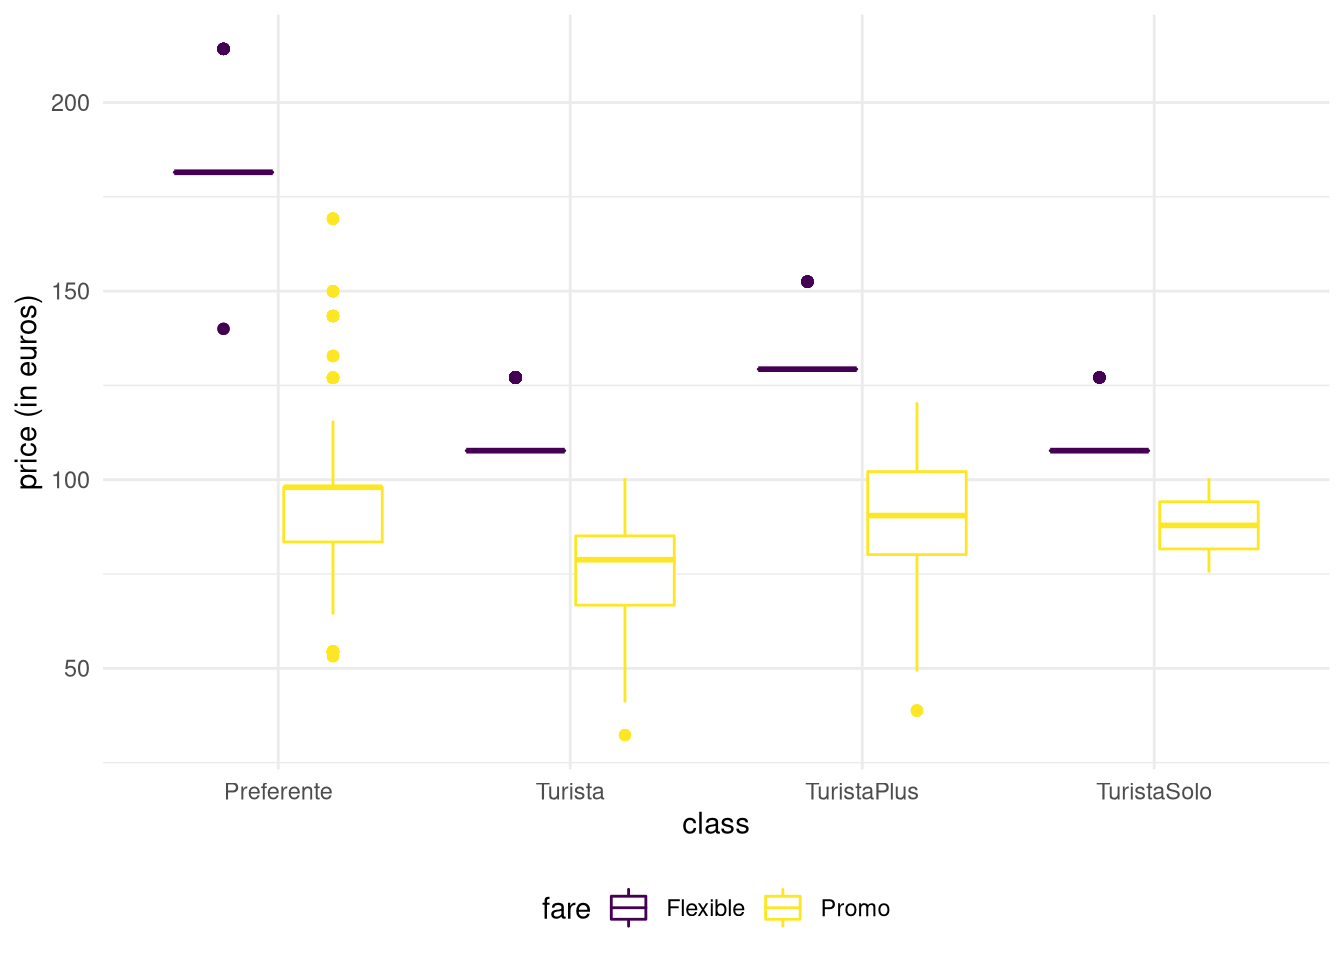
\includegraphics[width=0.7\linewidth]{MATH60604A_Statistical_modelling_files/figure-latex/renfe-aed6-1} 

}

\caption{Boxplot of ticket price as a function of fare and class for high-speed Renfe trains.}\label{fig:renfe-aed6}
\end{figure}

\begin{Shaded}
\begin{Highlighting}[]
\KeywordTok{ggplot}\NormalTok{(}\DataTypeTok{data =}\NormalTok{ renfe, }\KeywordTok{aes}\NormalTok{(}\DataTypeTok{x =}\NormalTok{ price, }\DataTypeTok{y=}\NormalTok{..density.., }\DataTypeTok{fill =}\NormalTok{ fare)) }\OperatorTok{+}
\StringTok{    }\KeywordTok{geom\_histogram}\NormalTok{(}\DataTypeTok{binwidth =} \DecValTok{5}\NormalTok{) }\OperatorTok{+}
\StringTok{    }\KeywordTok{labs}\NormalTok{(}\DataTypeTok{x =} \StringTok{"price (in euros)"}\NormalTok{, }\DataTypeTok{y =} \StringTok{"density"}\NormalTok{) }\OperatorTok{+}\StringTok{ }
\StringTok{    }\KeywordTok{theme}\NormalTok{(}\DataTypeTok{legend.position =} \StringTok{"bottom"}\NormalTok{)}
\end{Highlighting}
\end{Shaded}

\begin{figure}

{\centering 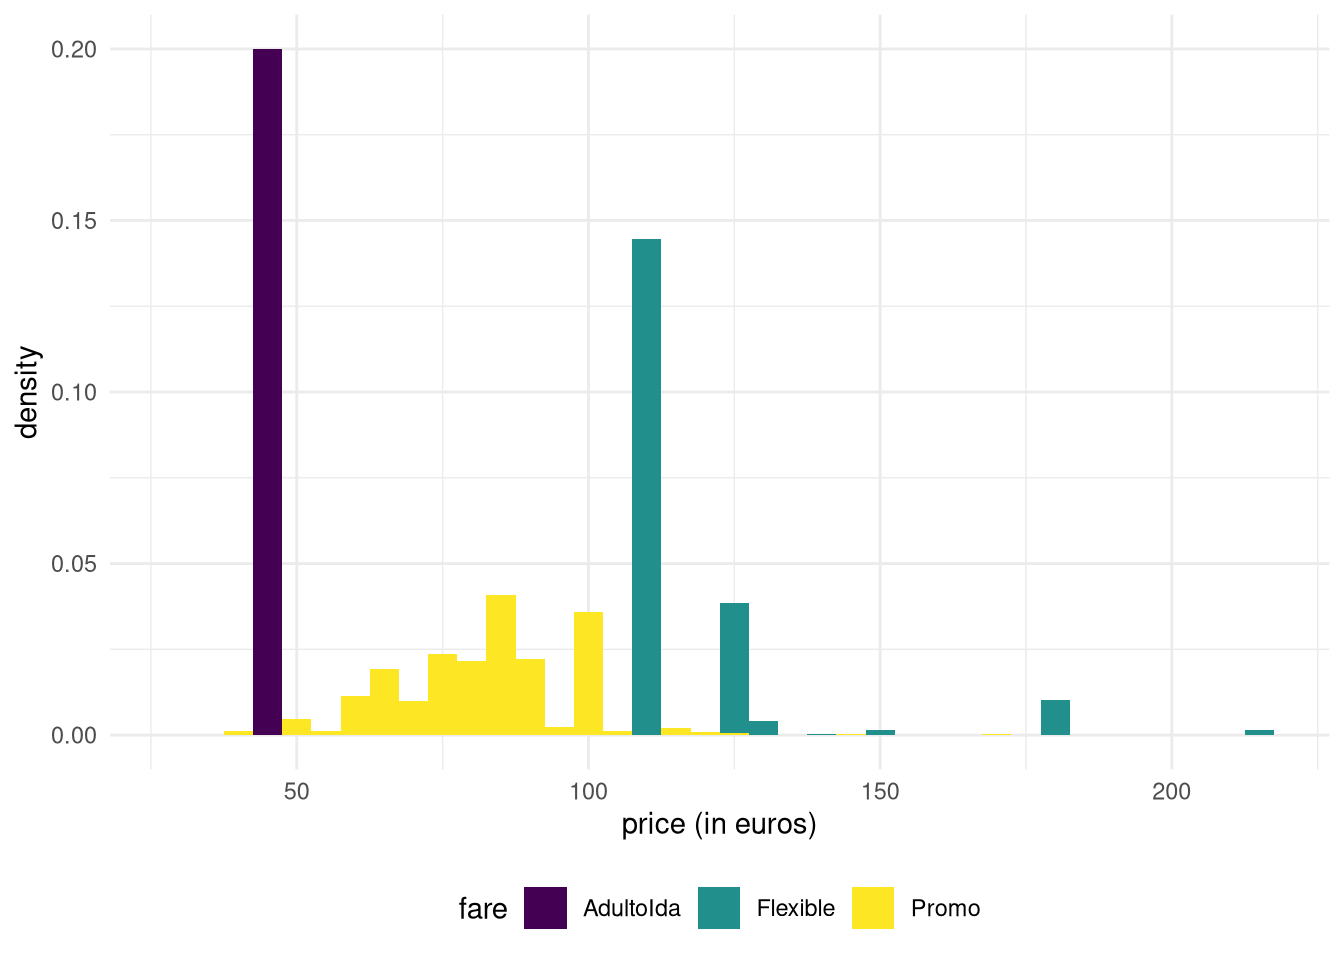
\includegraphics[width=0.7\linewidth]{MATH60604A_Statistical_modelling_files/figure-latex/renfe-aed7-1} 

}

\caption{Histograms of ticket price as a function of fare for Renfe trains.}\label{fig:renfe-aed7}
\end{figure}

\begin{Shaded}
\begin{Highlighting}[]
\CommentTok{\# Check the spread of Flexible tickets}
\NormalTok{renfe }\OperatorTok{\%\textgreater{}\%}\StringTok{ }\KeywordTok{subset}\NormalTok{(fare  }\OperatorTok{==}\StringTok{ "Flexible"}\NormalTok{) }\OperatorTok{\%\textgreater{}\%}\StringTok{ }\KeywordTok{count}\NormalTok{(price, class)}
\end{Highlighting}
\end{Shaded}

\begin{verbatim}
##   price       class    n
## 1   108     Turista 1050
## 2   108 TuristaSolo   67
## 3   127     Turista  285
## 4   127 TuristaSolo    9
## 5   129 TuristaPlus   31
## 6   140  Preferente    2
## 7   152 TuristaPlus   10
## 8   182  Preferente   78
## 9   214  Preferente   12
\end{verbatim}

Note how Flexible tickets prices are spread: the boxplot is crushed and the interquartile range seems zero, even if some of the values are larger: this is indicative either constant price or of (too few) tickets in the category. We can find out which of these two possibities is most likely by counting the number of Flexible fare tickets for the different types.

Neither duration, nor type or destination explains why some Flexible tickets are more or less expensive than the average. Promo tickets, on the other hand, are cheaper on average and Preferente more expensive.

We can summarize our findings:

\begin{itemize}
\tightlist
\item
  more than 91\% of trains are high-speed trains.
\item
  travel time depends on the type of train: high-speed train take at most 3h20.
\item
  duration records expected travel time: there are only 17 unique values, 13 of which are for AVE trains.
\item
  the price of RegioExpress train ticket is fixed (43.25€); all such tickets are sold with AdultoIda fare and there only one class (Turista). 57\% of these trains go from Barcelona to Madrid and travel time is 9h22 from Barcelona to Madrid, 9h04 in the other direction.
\item
  \texttt{Turista} is the cheapest and most popular class. \texttt{Preferente} class tickets are more expensive and are less often sold. \texttt{TuristaPlus} offers more comfort and \texttt{TuristaSolo} let you get individual seats.
\item
  according to the \href{https://www.renfe.com/es/es/viajar/tarifas/billetes.html}{Renfe website}, \texttt{Flexible} fare tickets ``come with additional offers and passengers can exchange or cancel their tickets if they miss their train''; as a counterpart, these tickets are more expensive and most tickets have a fixed fare (a handful are cheaper or more expensive, but this price difference is unexplained).
\item
  the distribution of \texttt{Promo} fare high-speed trains ticket prices are more or less symmetric, but \texttt{Flexible} tickets seem left-truncated (the minimum price for these tickets in the sample is 107.7€).
\item
  it appears that tickets sold by Renfe (\texttt{Promo} fare) are dynamically priced: the latter can be up to 70\% cheaper than regular high-speed train tickets when purchased through the official agency or Renfe's website. These tickets cannot be refunded or exchanged.
\item
  there is no indication that prices depend on the direction of travel.
\end{itemize}

\hypertarget{linear-regression}{%
\chapter{Linear regression}\label{linear-regression}}

A linear regression is a model for the conditional mean of a response variable \(Y\) as a function of \(p\) explanatory variables (also termed regressors or covariates),
\begin{align}
\mathsf{E}(Y \mid \mathbf{X})=\beta_0 + \beta_1\mathrm{X}_{1} + \cdots + \beta_p \mathrm{X}_{p}. \label{eq:linearreg}
\end{align}
The mean of \(Y\) is conditional on the values of the observed covariate \(\mathbf{X}\); this amounts to treating them as non-random, known in advance.

In practice, any model is an approximation of reality. An error term is included to take into account the fact that no exact linear relationship links \(\mathbf{X}\) and \(Y\) (otherwise this wouldn't be a statistical problem), or that measurements of \(Y\) are subject to error. The random error term \(\varepsilon\) will be the source of information for our inference, as it will quantify the goodness of fit of the model.

We can rewrite the linear model in terms of the error for a random sample of size \(n\): denote by \(Y_i\) the value of the response for observation \(i\), and \(\mathrm{X}_{ij}\) the value of of the \(j\)th explanatory variable of observation \(i\). The model is
\begin{align}
Y_i = \beta_0 + \beta_1 \mathrm{X}_{i1} + \ldots + \beta_p \mathrm{X}_{ip} +\varepsilon_{i}, \qquad i =1, \ldots, n, \label{eq:olsmean}
\end{align}
where \(\varepsilon_i\) is the additive error term specific to observation \(i\). While we may avoid making distributional assumption about \(\varepsilon_i\), we nevertheless fix its expectation to zero to encode the fact we do not believe the model is systematically off,, so \(\mathsf{E}(\varepsilon_i \mid \boldsymbol{X}_i)=0\) \((i=1, \ldots, n)\).

One important remark is that the model is linear in the coefficients \(\boldsymbol{\beta}\in \mathbb{R}_{p+1}\), not in the explanatory variables! the latter are arbitrary and could be (nonlinear) functions of other explanatory variables, for example \(\mathrm{X}=\ln(\texttt{years})\), \(\mathrm{X}=\texttt{horsepower}^2\) or \(\mathrm{X}= \mathsf{I}_{\texttt{man}}\cdot\mathsf{I}_{\texttt{full}}\). The mean of the response is specified as a \textbf{linear combination of explanatory variables}. This is at the core of the flexibility of the linear regression, which is used mainly for the following purposes:

\begin{enumerate}
\def\labelenumi{\arabic{enumi}.}
\tightlist
\item
  Evaluate the effects of covariates \(\mathbf{X}\) on the mean response
  of \(Y\).
\item
  Quantify the influence of the explanatories \(\mathbf{X}\) on the
  response and test for their significance.
\item
  Predict the response for new sets of explanatories \(\mathbf{X}\).
\end{enumerate}

\hypertarget{introduction}{%
\section{Introduction}\label{introduction}}

Linear regression is the most famous and the most widely used statistical model around. The name may appear reductive, but many tests statistics (\emph{t}-tests, ANOVA, Wilcoxon, Kruskal--Wallis) \href{https://lindeloev.github.io/tests-as-linear/linear_tests_cheat_sheet.pdf}{can be formulated using a linear regression}, while \href{https://threadreaderapp.com/thread/1286420597505892352.html}{models as diverse as trees, principal components and deep neural networks are just linear regression model in disguise}. What changes under the hood between one fancy model to the next are the optimization method (e.g., ordinary least squares, constrained optimization or stochastic gradient descent) and the choice of variables entering the model (spline basis for nonparametric regression, indicator variable selected via a greedy search for trees, activation functions for neural networks).

This chapter explores the basics of linear regression, parameter interpretation and testing for coefficients and sub-models. Analysis of variance will be presented as special case of linear regression.

To make concepts and theoretical notions more concrete, we will use data from a study performed in a college in the United States. The goal of the administration who collected these information was to investigate potential gender inequality in the salary of faculty members. The data contains the following variables:

\begin{itemize}
\tightlist
\item
  \texttt{salary}: nine-month salary of professors during the 2008--2009 academic year (in thousands USD).
\item
  \texttt{rank}: academic rank of the professor (\texttt{assistant}, \texttt{associate} or \texttt{full}).
\item
  \texttt{field}: categorical variable for the field of expertise of the professor, one of \texttt{applied} or \texttt{theoretical}.
\item
  \texttt{sex}: binary indicator for sex, either \texttt{man} or \texttt{woman}.
\item
  \texttt{service}: number of years of service in the college.
\item
  \texttt{years}: number of years since PhD.
\end{itemize}

Before drafting a model, a quick look at the data is in due order. If salary increases with year, there is more heterogeneity in the salary of higher ranked professors: logically, assistant professors are either promoted or kicked out after at most 6 years according to the data. The limited number of years prevents large variability for their salaries.

\begin{figure}

{\centering 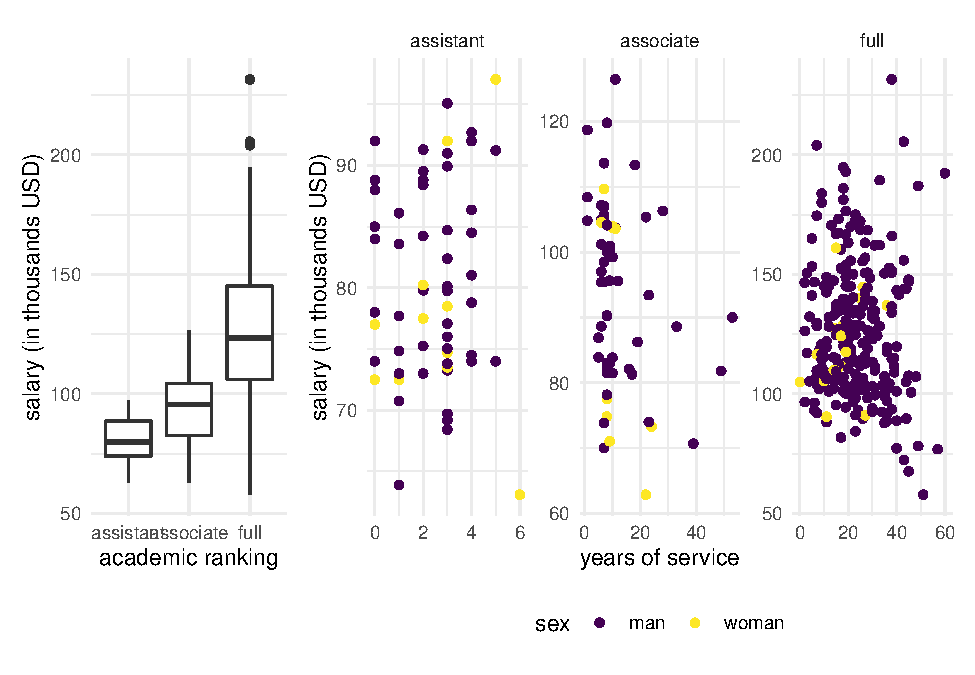
\includegraphics[width=0.7\linewidth]{MATH60604A_Statistical_modelling_files/figure-latex/edacollege-1} 

}

\caption{Exploratory data analysis of $\texttt{college}$ data: salaries of professors as a function of the number of years of service and the academic ranking}\label{fig:edacollege}
\end{figure}

Salary increases over years of service, but its variability also increases with rank. Note the much smaller number of women in the sample: this will impact our power to detect differences between sex. A contingency table of sex and academic rank can be useful to see if the proportion of women is the same in each rank: women represent 16\% of assistant professors and 16\% of associate profs, but only 7\% of full professors and these are better paid on average.

\begin{table}

\caption{\label{tab:tableaucontingence}Contingency table of the number of prof in the college by sex and academic rank.}
\centering
\begin{tabular}[t]{lrrr}
\toprule
  & assistant & associate & full\\
\midrule
man & 56 & 54 & 248\\
woman & 11 & 10 & 18\\
\bottomrule
\end{tabular}
\end{table}

The simple linear regression model only includes a single explanatory variable and defines a straight line linking two variables \(\mathrm{X}\) and \(Y\) by means of an equation of the form \(y=a+bx\); Figure \ref{fig:droitenuage} shows the line passing through the scatterplot for years of service.

\begin{figure}

{\centering 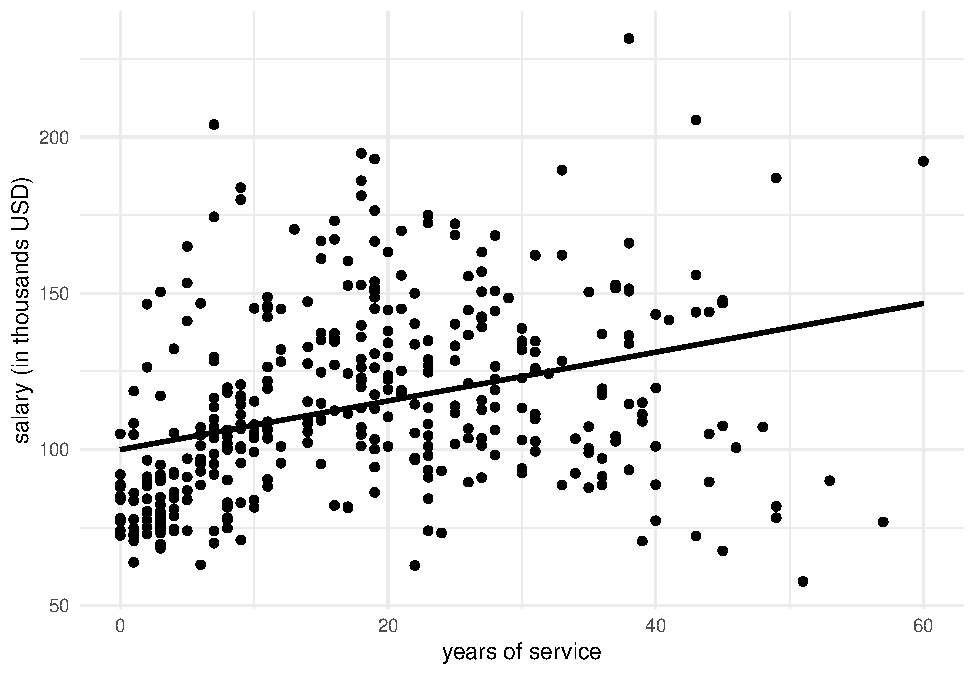
\includegraphics[width=0.7\linewidth]{MATH60604A_Statistical_modelling_files/figure-latex/droitenuage-1} 

}

\caption{Simple linear regression model for the salary of professors as a function of the number of years of service; the line is the solution of the least squares problem.}\label{fig:droitenuage}
\end{figure}

\hypertarget{ordinary-least-squares}{%
\section{Ordinary least squares}\label{ordinary-least-squares}}

The ordinary least square estimators \(\widehat{\boldsymbol{\beta}}=(\widehat{\beta}_0, \ldots, \widehat{\beta}_p)\) are the values that simultaneously minimize the Euclidean distance between the random observations \(Y_i\) and the \textbf{fitted values}
\begin{align*}
 \widehat{Y}_i &= \widehat{\beta}_0 + \widehat{\beta}_1 \mathrm{X}_{i1} + \cdots + \widehat{\beta}_p \mathrm{X}_{ip}, \qquad i =1, \ldots, n.
\end{align*}
In other words, the least square estimators are the solution of the convex optimization problem
\begin{align*}
\widehat{\boldsymbol{\beta}} &=\min_{\boldsymbol{\beta} \in \mathbb{R}^{p+1}}\sum_{i=1}^n (Y_i-\widehat{Y}_i)^2= \min_{\boldsymbol{\beta}} \|\boldsymbol{Y}-\mathbf{X}\boldsymbol{\beta}\|^2
\end{align*}
This system of equations has an explicit solution which is better expressed using matrix notation: this amounts to expressing equation \eqref{eq:olsmean} with one observation per line.

Consider the matrices
\begin{align*}
\boldsymbol{Y} =
 \begin{pmatrix}
  Y_1 \\
  Y_2 \\
  \vdots \\
  Y_n 
 \end{pmatrix} ,
 \;
 \boldsymbol{\varepsilon} =
 \begin{pmatrix}
  \varepsilon_1 \\
  \varepsilon_2 \\
  \vdots \\
  \varepsilon_n 
 \end{pmatrix} ,
 \;
\mathbf{X} = \begin{pmatrix}
\mathrm{X}_{11} & \mathrm{X}_{12} & \cdots & \mathrm{X}_{1p} \\
\mathrm{X}_{21} & \mathrm{X}_{22} & \cdots & \mathrm{X}_{2p} \\
\vdots & \vdots & \ddots & \vdots \\
\mathrm{X}_{n1} & \mathrm{X}_{n2} & \cdots & \mathrm{X}_{np} 
\end{pmatrix} , \;
\boldsymbol{\beta} =
 \begin{pmatrix}
  \beta_1 \\
  \beta_2 \\
  \vdots \\
  \beta_p 
 \end{pmatrix}
\end{align*}
The model in compact form is
\begin{align*}
\boldsymbol{Y} = \mathbf{X} \boldsymbol{\beta} + \boldsymbol{\varepsilon}.
\end{align*}
The ordinary least squares estimator solves the unconstrained optimization problem
\begin{align*}
\widehat{\boldsymbol{\beta}}=\min_{\boldsymbol{\beta} \in \mathbb{R}^{p+1}}(\boldsymbol{y}-\mathbf{X}\boldsymbol{\beta})^\top(\boldsymbol{y}-\mathbf{X}\boldsymbol{\beta}).
\end{align*}
and a proof is provided \protect\hyperlink{ols}{in the Appendix}. If the \(n \times (p+1)\) matrix \(\mathbf{X}\) is full-rank, we obtain a unique solution to the optimization problem,
\begin{align}
\widehat{\boldsymbol{\beta}} = (\mathbf{X}^{\top} \mathbf{X})^{-1} \mathbf{X}^{\top} \boldsymbol{Y}. \label{eq:ols}
\end{align}

What does the solution to the least squares problem represent in two dimensions? The estimator is the one minimizing the sum of squared residuals: the \(i\)th \textbf{ordinary residual} \(e_i = y_i -\widehat{y}_i\) is the \emph{vertical} distance between a point \(y_i\) and the fitted value \(\widehat{y}_i\) on the line; the blue segments on Figure \ref{fig:distancevert} represent the individual vectors of residuals.

\begin{figure}

{\centering 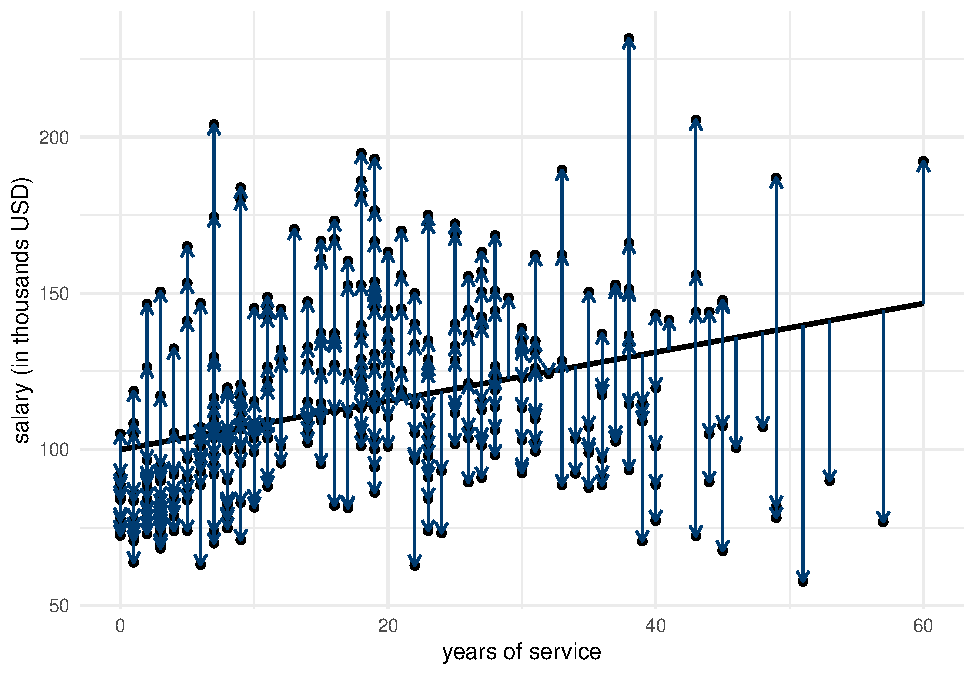
\includegraphics[width=0.7\linewidth]{MATH60604A_Statistical_modelling_files/figure-latex/distancevert-1} 

}

\caption{Illustration of ordinary residuals added to the regression line (blue vectors).}\label{fig:distancevert}
\end{figure}

\begin{remark}[Geometry of least squares]
\iffalse{} {Remark (Geometry of least squares). } \fi{}If we consider the \(n\) observations as a (column) vector, the term \(\mathbf{X} \widehat{\boldsymbol{\beta}}\) is the projection of the response vector \(\boldsymbol{y}\) on the linear span generated by the columns of \(\mathbf{X}\), \(\mathscr{S}_{\mathbf{X}}\). The ordinary residuals are thus orthogonal to \(\mathscr{S}_{\mathbf{X}}\) and to the fitted values, meaning \(\boldsymbol{e}^\top\widehat{\boldsymbol{y}}=0\).
A direct consequence of this fact is that the linear correlation between \(\boldsymbol{e}\) and \(\widehat{\boldsymbol{y}}\) is zero; we will use this property to build graphical diagnostics.
\end{remark}

\begin{remark}[Complexity of ordinary least squares]
\iffalse{} {Remark (Complexity of ordinary least squares). } \fi{}This is an aside: in machine learning, you will often encounter linear models fitted using a (stochastic) gradient descent algorithm. Unless your sample size \(n\) or the number of covariates \(p\) is significant (think at the Google scale), an approximate should not be prefered to the exact solution! From a numerical perspective, obtaining the least square estimates requires inverting a \((p+1) \times (p+1)\) matrix \(\mathbf{X}^\top\mathbf{X}\), which is the most costly operation. In general, direct inversion should be avoided because it is not the most numerically stable way of obtaining the solution. \textbf{R} uses the QR decomposition, which has a complexity of \(\mathrm{O}(np^2)\). Another more stable alternative, which has the same complexity but is a bit more costly is use of a singular value decomposition.
\end{remark}

Any good software will calculate ordinary least square estimates for you. Keep in mind that there is an explicit and unique solution provided your model matrix \(\mathbf{X}\) doesn't contain collinear columns. If you have more than one explanatory variable, the fitted values lie on a hyperplan (which is hard to represent graphically). Mastering the language and technical term (fitted values, ordinary residuals, etc.) is necessary for the continuation.

\hypertarget{interpretation-of-the-model-parameters}{%
\section{Interpretation of the model parameters}\label{interpretation-of-the-model-parameters}}

What do the \(\boldsymbol{\beta}\) parameters of the linear model represent? In the simple case presented in Figure \ref{fig:droitenuage}, the equation of the line is \(\widehat{Y} = \widehat{\beta}_0 + \widehat{\beta}_1\mathrm{X}_1\), \(\beta_0\) is the intercept (the mean value of \(Y\) when \(\mathrm{X}_1=0\)) and \(\beta_1\) is the slope, i.e., the average increase of \(Y\) when \(\mathrm{X}_1\) increases by one unit.

In some cases, the intercept is \textbf{meaningless} because the value \(\mathrm{X}_1=0\) is impossible (e.g., \(\mathrm{X}_1\) represents the height of a human). In the same vein, there may be no observation in a neighborhood of \(\mathrm{X}_1=0\), even if this value is plausible, in which case the intercept is an \textbf{extrapolation}.

If the columns of \(\mathbf{X}\) are arbitrary, it is customary to include an intercept: this amounts to including \(\mathbf{1}_n\) as column of the model matrix \(\mathbf{X}\). Because the residuals are orthogonal to the columns of \(\mathbf{X}\), their mean is zero, since \(n^{-1}\mathbf{1}_n^\top\boldsymbol{e}=\bar{\boldsymbol{e}}=0\). In general, we could also obtain mean zero residuals by including a set of vectors in \(\mathbf{X}\) that span \(\mathbf{1}_n\).

In our example, the equation of the fitted line of Figure \ref{fig:droitenuage} is \[\widehat{\texttt{salary}} = 99.975 + 0.78\texttt{service}.\]
The average salary of a new professor would then be 99974.653 dollars, whereas the average annual increase for each additional year of service is 779.569 dollars.

If the response variable \(Y\) should be continuous (for the least square criterion to be meaningful), we place no such restriction on the explanatories. The case of dummies in particular is common: these variables are encoded using binary indicators (\(0/1\)). Consider for example the sex of the professors in the study:
\[\texttt{sex} = \begin{cases} 0 , & \text{for men},\\
1, & \text{for women.}
\end{cases}
\]
The equation of the simple linear model that includes the binary variable \(\texttt{sex}\) is \(\texttt{salary} = \beta_0 + \beta_1 \texttt{sex} + \varepsilon\). Let \(\mu_0\) denote the average salary of mean and \(\mu_1\) that of women. The intercept \(\beta_0\) can be interpreted as usual: it is the average salary when \(\texttt{sex}=0\), meaning that \(\beta_0=\mu_0\). We can write the equation for the conditional expectation for each sex,
\begin{align*}
\mathsf{E}(\texttt{salary} \mid \texttt{sex})= \begin{cases}
\beta_0, & \texttt{sex}=0 \text{ (men)}, \\
\beta_0 + \beta_1 & \texttt{sex}=1 \text{ (women)}.
\end{cases}
\end{align*}
A linear model that only contains a binary variable \(\mathrm{X}\) as regressor amounts to specifying a different mean for each of two groups: the average of women is \(\mathsf{E}(\texttt{salary} \mid \texttt{sex}=1) = \beta_0 + \beta_1 = \mu_1\) and \(\beta_1=\mu_1-\mu_0\) represents the difference between the average salary of men and women. The least square estimator \(\widehat{\beta}_0\) is the sample mean of men and \(\widehat{\beta}_1\) is the difference of the sample mean of women and men. The parametrization of the linear model with \(\beta_0\) and \(\beta_1\) is in terms of \textbf{contrasts} and is particularly useful if we want to test for mean difference between the groups, as this amounts to testing \(\mathscr{H}_0: \beta_1=0\). If we wanted our model to directly output the sample means, we would need to replace the model matrix \(\mathbf{X}=[\mathbf{1}_n, \texttt{sex}]\) by \([\mathbf{1}_n- \texttt{sex}, \texttt{sex}]\). The fitted model would be the same because they span the same 2D subspace, but this is not recommended because software treat cases without intercept differently and it can lead to unexpected behaviour (more on this latter).

\begin{figure}

{\centering 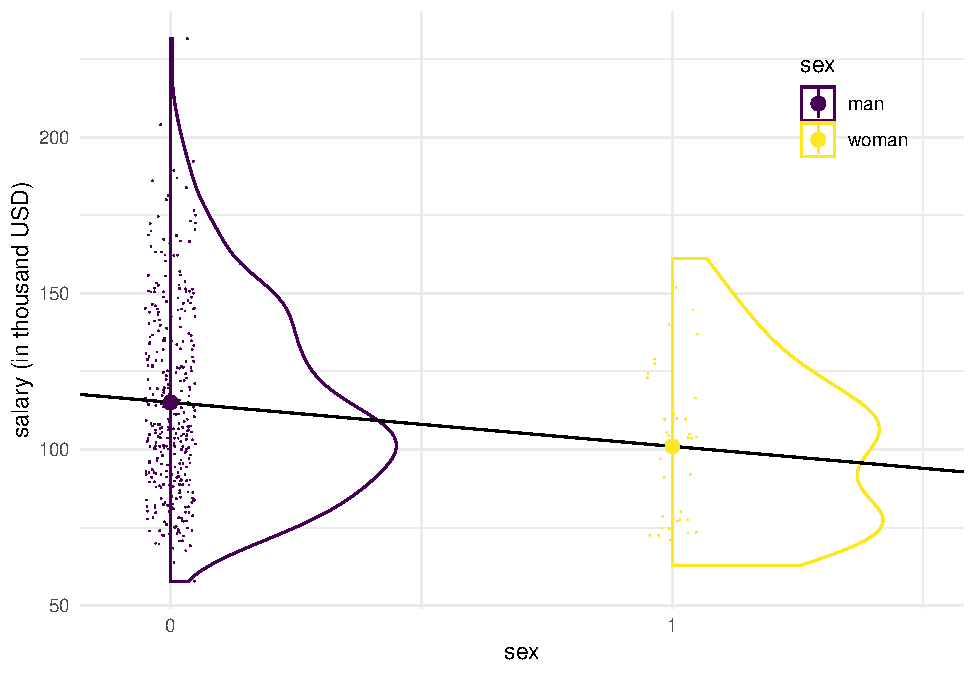
\includegraphics[width=0.7\linewidth]{MATH60604A_Statistical_modelling_files/figure-latex/graphcollegesex-1} 

}

\caption{Simple linear model for the $\texttt{college}$ data using the binary variable sex as regressor: even if the equation defines a line, only its values in $0/1$ are realistic.}\label{fig:graphcollegesex}
\end{figure}

If we fit the model with sex only to the \texttt{college} data, we find that the average salary of men is \(\widehat{\beta}_0=\ensuremath{1.151\times 10^{5}}\) USD and the mean difference estimate of the salary between women and men is \(\widehat{\beta}_1=14088.009\) dollars. Since the estimate is negative, this means women are paid less. Bear in mind that the model is not adequate for determining if there are gender inequalities in the salary distribution: \ref{fig:droitenuage} shows that the number of years of service and the academic rank strongly impact wages, yet the distribution of men and women is not the same within each rank.

Even if the linear model defines a line, the latter is only meaningful when evaluated at \(0\) or \(1\); Figure \ref{fig:graphcollegesex} shows it in addition to sample observations (jittered) and a density estimate for each sex. The colored dot represents the mean, showing that the line does indeed pass through the mean of each group.

A binary indicator is a categorical variable with two levels, so we could extend our reasoning and fit a model with a categorical explanatory variable with \(k\) levels. To do this, we add \(k-1\) indicator variables plus the intercept: if we want to model a different mean for each of the \(k\) groups, it is logical to only include \(k\) parameters in the mean model. We will choose, as we did with sex, a \textbf{reference category} or \textbf{baseline} whose average will be encoded by the intercept \(\beta_0\). The other parameters \(\beta_1, \ldots, \beta_{k-1}\) are contrasts relative to the baseline. The college data includes the ordinal variable \texttt{rank}, which has three levels (assistant, associate and full). We thus need two binary variables, \(\mathrm{X}_1 = \mathsf{I}(\texttt{rank}=\texttt{associate})\) and \(\mathrm{X}_2 = \mathsf{I}(\texttt{rank}=\texttt{full})\); the \(i\)th element of the vector \(\mathrm{X}_1\) is one for an associate professor and zero otherwise. The linear model is
\begin{align*}
\texttt{salary} =\beta_0 + \beta_1 \mathrm{X}_1+\beta_2\mathrm{X}_2 + \varepsilon,
\end{align*}
and the conditional expectation of salary
\begin{align*}
\mathsf{E}(\texttt{salary} \mid \texttt{rank})= \begin{cases}
\beta_0, & \texttt{rank}=\texttt{assistant},\\
\beta_0 + \beta_1 & \texttt{rank}=\texttt{associate},\\
\beta_0 + \beta_2 & \texttt{rank}=\texttt{full},
\end{cases}
\end{align*}
Thus \(\beta_1\) (respectively \(\beta_2\)) are the difference between the average salary of associate (respectively full) professors and assistant professors. The choice of the baseline category is arbitrary and all choices yield the same model: only the interpretation changes from one parametrization to the next. For an ordinal variable, it is recommended to choose the smallest or the largest category to ease comparisons.

The models we have fitted so far are not adequate because they ignore variables that are necessarily to correctly explain variations in salaries: Figure \ref{fig:edacollege} show for example that rank is critical for explaining the salary variations in the college. We should thus fit a model that include those simultaneously to investigate the gender gap (which consists of differences that are unexplained by other factors). Before doing this, we come back to the interpretation of the parameters in the multiple linear regression setting.

Consider the model \(Y= \beta_0 + \beta_1 \mathrm{X}_1 + \cdots + \beta_p\mathrm{X}_p + \varepsilon\). The intercept \(\beta_0\) represents the mean value of \(Y\) when \emph{all} of the covariates are set to zero,
\begin{align*}
\beta_0 &= \mathsf{E}(Y \mid \mathrm{X}_1=0,\mathrm{X}_2=0,\ldots,\mathrm{X}_p=0).
\end{align*}
For categorical variables, this yields the baseline, whereas we fix the continous variables to zero: again, this may be nonsensical depending on the study. The coefficient \(\beta_j\) \((j \geq 1)\) can be interpreted as the mean increase of the response \(Y\) when \(\mathrm{X}_j\) increases by one unit, all other things being equal (\emph{ceteris paribus}); e.g.,
\begin{align*}
\beta_1 &= \mathsf{E}(Y \mid \mathrm{X}_1=x_1+1,\mathrm{X}_2=x_2,\ldots,\mathrm{X}_p=x_p) \\
& \qquad \qquad - \mathsf{E}(Y \mid \mathrm{X}_1=x_1,\mathrm{X}_2=x_2,\ldots,\mathrm{X}_p=x_p) \\
&= \left\{\beta_0 + \beta_1 (x_1+1) + \beta_2 x_2 + \cdots +\beta_p \mathrm{X}_p \right\} \\
& \qquad \qquad -\left\{\beta_0 + \beta_1 x_1 + \beta_2 x_2 + \cdots +\beta_p \mathrm{X}_p \right\} 
\end{align*}
It is not always possible to fix the value of an explanatory if multiple columns of \(\mathbf{X}\) contains functions/transformations of it. For example, if we included a polynomial of order \(k\) for some variable \(\mathrm{X}\),
\begin{align*}
Y=\beta_0+ \beta_1 \mathrm{X}+ \beta_2 \mathrm{X}^2 + \ldots +\beta_k \mathrm{X}^k + \varepsilon.
\end{align*}
If we include a term of order \(k\), \(\mathrm{X}^k\), we must \emph{always} include the lower order terms \(1, \mathrm{X}, \ldots, \mathrm{X}^{k-1}\) to make sure the resulting model is interpretable (otherwise, it amounts to a particular class of polynomials with some zero coefficients). Interpreting nonlinear effects (even polynomials, for which \(k\leq 3\) in practice), is complicated because the effect of an increase of one unit of \(\mathrm{X}\) \emph{depends of the value of the latter}.

\begin{example}[Auto data]
\protect\hypertarget{exm:auto}{}{\label{exm:auto} \iffalse (Auto data) \fi{} }We consider a linear regression model for the fuel autonomy of cars as a function of the power of their motor (measured in horsepower) from the \texttt{auto} dataset. The postulated model,
\[
\texttt{mpg}_i = \beta_0 + \beta_1 \texttt{horsepower}_i + \beta_2 \texttt{horsepower}_i^2 + \varepsilon_i,
\]
includes a quadratic term. Figure \ref{fig:autoquad2d} shows the scatterplot with the fitted regression line, above which the line for the simple linear regression for horsepower is added.
\end{example}

\begin{figure}

{\centering 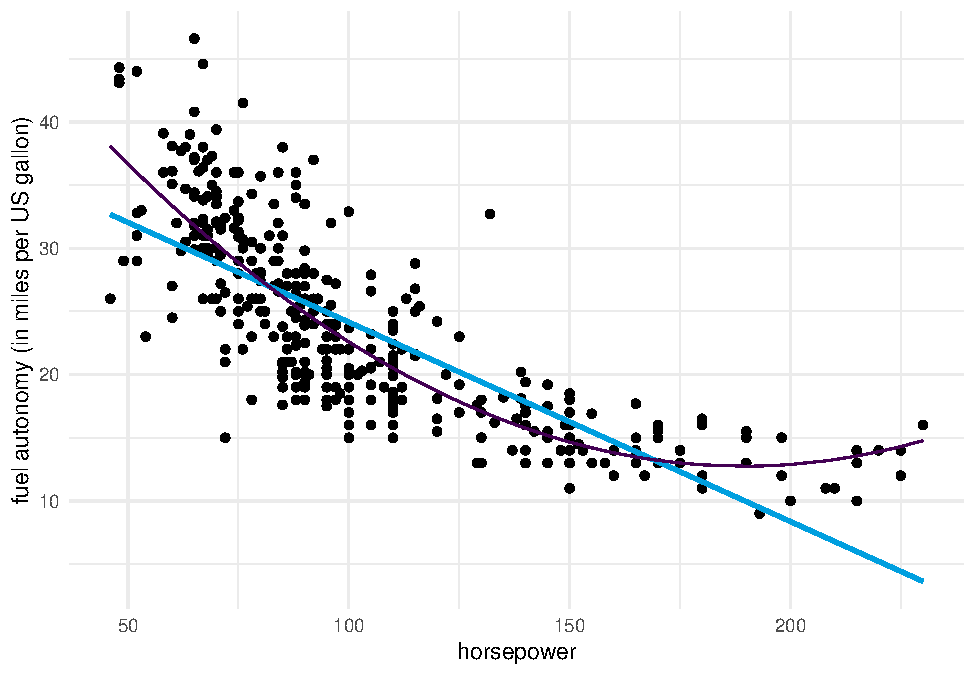
\includegraphics[width=0.7\linewidth]{MATH60604A_Statistical_modelling_files/figure-latex/autoquad2d-1} 

}

\caption{Linear regression models for the fuel autonomy of cars as a function of motor power}\label{fig:autoquad2d}
\end{figure}

It appears graphically that the quadratic model fits better than the simple linear alternative: we will assess this hypothesis formally later. For the degree two polynomial, Figure \ref{fig:autoquad2d} show that fuel autonomy decreases rapidly when power increases between 50 to 100, then more slow until 189.35 hp. After that, the model postulates that autonomy increases again as evidenced by the scatterplot, but beware of extrapolating (weird things can happen beyond the range of the data, as exemplified by \href{https://livefreeordichotomize.com/2020/05/05/model-detective/}{Hassett's cubic model for the number of daily cases of Covid19 in the USA}).

The representation in Figure \ref{fig:autoquad2d} may seem counter-intuitive given that we fit a linear model, but it is a 2D projection of 3D coordinates for the equation \(\beta_0 + \beta_1x-y +\beta_2z =0\), where \(x=\texttt{horsepower}\), \(z=\texttt{horsepower}^2\) and \(y=\texttt{mpg}\). Physics and common sense force \(z = x^2\), and so the fitted values lie on a curve in a 2D subspace of the fitted plan, as shown in grey in the 3D Figure \ref{fig:hyperplan}.

\begin{figure}

{\centering 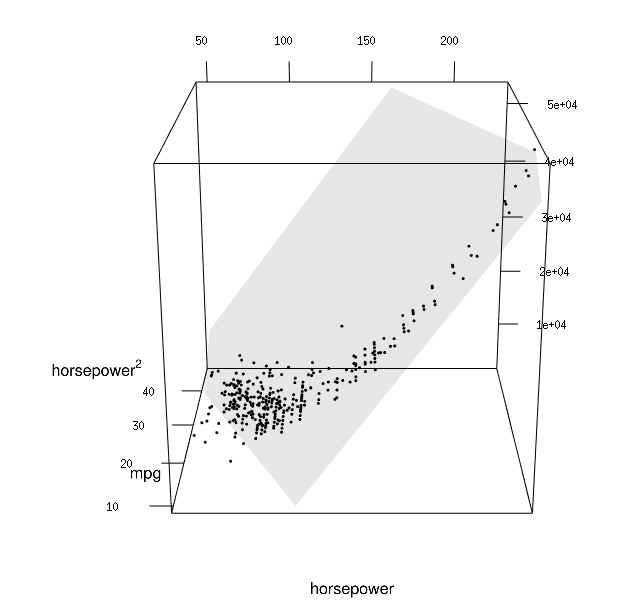
\includegraphics[width=0.7\linewidth]{images/hyperplane_auto} 

}

\caption{3D graphical representation of the linear regression model for the $\texttt{auto}$ data.}\label{fig:hyperplan}
\end{figure}

\begin{remark}[There are better alternatives to polynomials for modelling nonlinear effects]
\iffalse{} {Remark (There are better alternatives to polynomials for modelling nonlinear effects). } \fi{}Generally speaking, one uses flexible basis vectors (splines) rather than polynomials for smoothing when the relation between the response \(Y\) and an explanatory variable \(\mathrm{X}\) is nonlinear; these models involve many covariates and it is customary to add a penalty term to control for overfitting and wiggliness. A better (physical) understanding of the system, or a theoretical model can also guide the choice of functions to use.
\end{remark}

The coefficient \(\beta_j\) in Eq. \eqref{eq:linearreg} represents the \emph{marginal} contribution of \(\mathrm{X}_j\) when all the other covariates are included in the model and which is not explained by them. This can be represented graphically by projecting \(Y\) and \(\mathrm{X}_j\) in the orthogonal complement of \(\mathbf{X}_{-j}\) (the matrix containing all but the \(j\)th column \(\mathrm{X}_j\)). The \textbf{added-variable plot} is a graphical tool showing this projection: the residuals from the linear regression of \(Y\) onto \(\mathscr{S}(\mathbf{X}_{-j})\) are mapped to the \(y\)-axis, whereas the residuals from the linear regression of \(\mathrm{X}_j\) as a function of \(\mathbf{X}_{-j}\) are shown on the \(x\)-axis. The regression line passes through (\(0,0\)) and its slope is \(\widehat{\beta}_j\). This graphical diagnostic is useful for detecting collinearity and the impact of outliers.

\begin{example}[Wage inequality in an American college]
\protect\hypertarget{exm:inequite-salariale}{}{\label{exm:inequite-salariale} \iffalse (Wage inequality in an American college) \fi{} }We consider a multiple regression model for the \texttt{college} data that includes sex, academic rank, field of study and the number of years of service as regressors.
\end{example}

If we multiply \(\texttt{salary}\) by a thousand to get the resulting estimates in US dollars, the postulated model is
\begin{align*}
\texttt{salary}\times 1000 &= \beta_0 + \beta_1 \texttt{sex}_{\texttt{woman}} +\beta_2 \texttt{field}_{\texttt{theoretical}} \\&\quad +\beta_3 \texttt{rank}_{\texttt{associate}}
+\beta_4 \texttt{rank}_{\texttt{full}}  +\beta_5 \texttt{service} + \varepsilon.
\end{align*}

\begin{table}

\caption{\label{tab:collegecoefs}Estimated coefficients of the linear model for the $\texttt{college}$ (in USD, rounded to the nearest dollar).}
\centering
\begin{tabular}[t]{rrrrrr}
\toprule
$\widehat{\beta}_0$ & $\widehat{\beta}_1$ & $\widehat{\beta}_2$ & $\widehat{\beta}_3$ & $\widehat{\beta}_4$ & $\widehat{\beta}_5$\\
\midrule
86596 & -4771 & -13473 & 14560 & 49160 & -89\\
\bottomrule
\end{tabular}
\end{table}

The interpretation of the coefficients is as follows:

\begin{itemize}
\tightlist
\item
  The estimated intercept is \(\widehat{\beta}_0=86596\) dollars; it corresponds to the mean salary of men assistant professors who just started the job and works in an applied domain.
\item
  everything else being equal (same field, academic rank, and number of years of service), the estimated salary difference between a woman and is estimated at \(\widehat{\beta}_1=-4771\) dollars.
\item
  \emph{ceteris paribus}, the salary difference between a professor working in a theoretical field and one working in an applied field is \(\beta_2\) dollars: our estimate of this difference is \(-13473\) dollars, meaning applied pays more than theoretical.
\item
  \emph{ceteris paribus}, the estimated mean salary difference between associate and assistant professors is \(\widehat{\beta}_3=14560\) dollars.
\item
  \emph{ceteris paribus}, the estimated mean salary difference between full and assistant professors is \(\widehat{\beta}_4=49160\) dollars.
\item
  au sein d'un même échelon, chaque année supplémentaire de service mène à une augmentation de salary annuelle moyenne de \(\widehat{\beta}_5=-89\) dollars.
\end{itemize}

All other factors taken into account, women get paid less than men. It remains to see if this difference is statistically significant. Perhaps more surprising, the model estimates that salary decreases with every additional year of service: this seems counterintuitive when looking at Figure \ref{fig:droitenuage}, which showed a steady increas of salary over the years. However, this graphical representation is misleading because Figure \ref{fig:edacollege} showed that academic ranking mattered the most. Once all the other factors are accounted for, years of service serves to explain the salary of full professors who have been working unusual amounts of time and who gain less than the average full professor, as shown by the added-variable plot of Figure \ref{fig:avplotcollege}.

\begin{figure}

{\centering 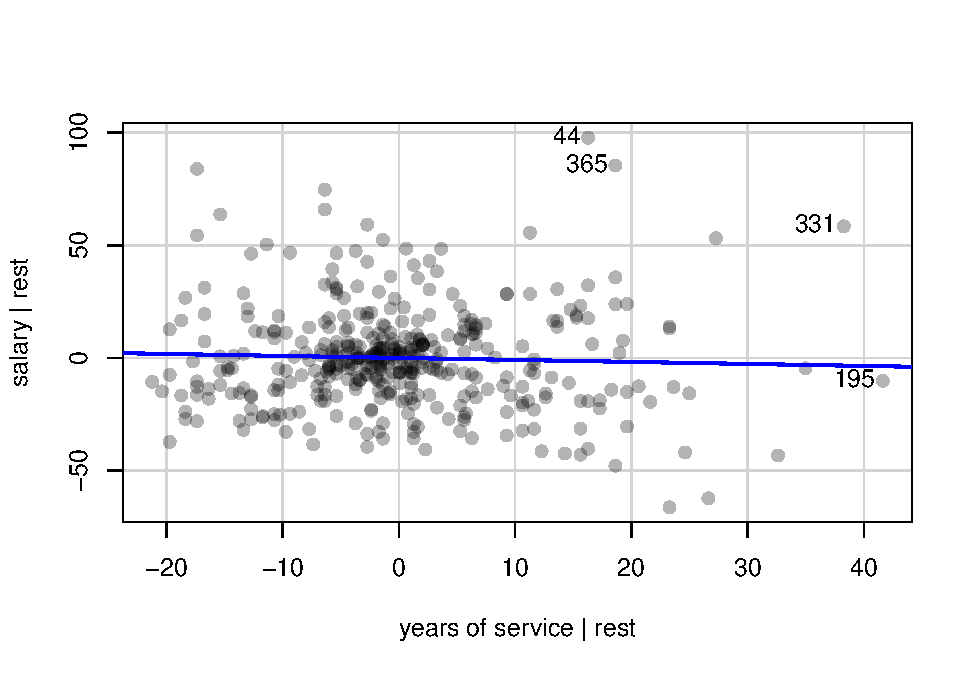
\includegraphics[width=0.7\linewidth]{MATH60604A_Statistical_modelling_files/figure-latex/avplotcollege-1} 

}

\caption{Added-variable plot for years of service in the linear regression model of the  $\texttt{college}$ data.}\label{fig:avplotcollege}
\end{figure}

\protect\hyperlink{rlmfunc}{Details about implementation of linear models using \textbf{R} are provided in the Appendix}.

\hypertarget{test-lm}{%
\section{Tests for parameters of the linear model}\label{test-lm}}

We need to make further assumptions in order to carry out inference and build testing procedures for the mean model parameters of the linear model. In order to get a tractable distribution for test statistics, it is customary to assume that the disturbances \(\boldsymbol{\varepsilon}\) are independent normal random variables with mean zero and common variance \(\sigma^2\). It follows that \(Y_1, \ldots, Y_n\) are conditionally \emph{independent} random variables with
\begin{align*}
\mathsf{E}(Y_i \mid \mathbf{X}_i)=\beta_0 + \sum_{j=1}^p \mathrm{X}_{ij}\beta_j, \quad  \mathsf{Va}(Y_i\mid \mathbf{X}_i)= \sigma^2, \quad i=1, \ldots, n.    
\end{align*}
Under this hypothesis, the least square estimators for the mean parameters coincide with the maximum likelihood estimators. The advantage of imposing this (more stringent than necessary) assumption is that we can use our toolbox for testing. The theory underlying likelihood tests is presented in the chapter on \href{likelihood}{likelihood-based inference}. Assuming normal errors leads to exact distributions for the test statistics (which also coincide with the asymptotic ones in large samples).

Of particular interest are tests of restrictions for components of \(\boldsymbol{\beta}\). The large sample properties of the maximum likelihood estimator imply that
\begin{align*}
\widehat{\boldsymbol{\beta}} \stackrel{\cdot}{\sim}\mathsf{No}_{p+1}\left\{\boldsymbol{\beta}, \sigma^2(\mathbf{X}^\top\mathbf{X})^{-1}\right\}
\end{align*}
for sufficiently large sample size. One can thus easily estimate the standard errors from the matrix upon replacing \(\sigma^2\) by an estimator, typically the unbiased estimator of the variance.

In an inferential setting, it's often important to test whether the effect of an explanatory variable is significant: if \(\mathrm{X}_j\) is binary or continuous, the test for \(\mathscr{H}_0: \beta_j=0\) corresponds to a null marginal effect for \(\mathrm{X}_j\). The null model is a linear regression in which we remove the \((j+1)\)st column of \(\mathbf{X}\), so both models are nested. The Wald test statistic is reported by most software \(W=\widehat{\beta}_j/\mathsf{se}(\widehat{\beta}_j)\) and the null distribution is Student-\emph{t} with \(n-p-1\) degrees of freedom, which explains the terminology (\(t\) values). In addition to coefficient estimates, it is possible to obtain confidence intervals for \(\beta_j\), which are the usual \(\widehat{\beta}_j \pm t_{n-p-1,\alpha/2} \mathsf{se}(\widehat{\beta}_j)\), with \(t_{n-p-1,\alpha/2}\) denoting the \(1-\alpha/2\) quantile of the \(\mathsf{St}_{n-p-1}\) distribution.

For categorical variables with more than two levels, testing if \(\beta_j=0\) is typically not of interest because the contrast represent the different between the category \(\mathrm{X}_j\) and the baseline: these two categories could have a small difference, but the categorical variable as a whole may still be a useful predictor given the other explanatories. The hypothesis of zero contrast is awkward because it implies a null model in which selected categories are merged.

\hypertarget{ftestslm}{%
\subsection{\texorpdfstring{\emph{F}-tests for comparison of nested linear models}{F-tests for comparison of nested linear models}}\label{ftestslm}}

Consider the \emph{full} linear model which contains \(p\) predictors,
\begin{align*}
\mathbb{M}_1: Y=\beta_0+\beta_1 \mathrm{X}_1 + \cdots + \beta_g \mathrm{X}_g + \beta_{k+1}\mathrm{X}_{k+1} + \ldots + \beta_p \mathrm{X}_p + \varepsilon.
\end{align*}
Suppose without loss of generality that we want to test \(\mathscr{H}_0: \beta_{k+1}=\beta_{k+2}=\ldots=\beta_p=0\) (one could permute columns of the model matrix to achieve this configuration).
The global hypothesis specifies that \((p-k)\) of the \(\beta\) parameters are zero. The \emph{restricted model} corresponding to the null hypothesis contains only the covariates for which \(\beta_j \neq 0\),
\begin{align*}
\mathbb{M}_0: Y=\beta_0+\beta_1 \mathrm{X}_1 + \ldots + \beta_k \mathrm{X}_k + \varepsilon.
\end{align*}
Let \(\mathsf{SS}_e(\mathbb{M}_1)\) be the residuals sum of squares for model \(\mathbb{M}_1\),
\begin{align*}
\mathsf{SS}_e(\mathbb{M}_1)=\sum_{i=1}^n (Y_i-\widehat{Y}_i^{\mathbb{M}_1})^2,
\end{align*}
where \(\widehat{Y}_i^{\mathbb{M}_1}\) is the \(i\)th fitted value from \(\mathbb{M}_1\). Similarly define \(\mathsf{SS}_e(\mathbb{M}_0)\) for the residuals sum of square of \(\mathbb{M}_0\). Clearly, \(\mathsf{SS}_e(\mathbb{M}_0) \geq \mathsf{SS}_e(\mathbb{M}_1)\) (why?)

The \(F\)-test statistic is
\begin{align*}
F=\frac{\{\mathsf{SS}_e(\mathbb{M}_0)-\mathsf{SS}_e(\mathbb{M}_1)\}/(p-k)}{\mathsf{SS}_e(\mathbb{M}_1)/(n-p-1)}
\end{align*}
Under \(\mathscr{H}_0\), the \(F\) statistic follows a \href{https://en.wikipedia.org/wiki/F-distribution}{Fisher distribution} with \((p-k)\) and \((n-p-1)\) degrees of freedom, \(\mathsf{F}(p-k, n-p-1)\) --- \(p-k\) is the number of restrictions, \(n-p-1\) is sample size minus the number of \(\beta\)'s in \(\mathbb{M}_1\).

It turns out that both \(F\) and \(t\)-statistics are equivalent for testing a single coefficient \(\beta_j\): the \(F\)-statistic is the square of the Wald statistic and they lead to the same inference --- the \(p\)-value for the test are identical. While it may get reported in tables, the test for \(\beta_0=0\) is not of interest; we keep the intercept merely to centre the residuals.

For normal linear regression, the likelihood ratio test for comparing models \(\mathbb{M}_1\) and \(\mathbb{M}_0\) is a function of the sum of squared residuals: the usual formula simplifies to \(R = n\ln\{\mathsf{SS}_e(\mathbb{M}_0)/\mathsf{SS}_e(\mathbb{M}_1)\}\). This is reminiscent of the \(F\)-statistic formula and the two are in fact intimately related modulo null distribution and scaling. The \(t\)-tests and \(F\)-tests presented above could thus both be viewed as particular cases of \href{liktests}{likelihood-based tests}.

Consider the \texttt{college} data example and the associated linear model with \texttt{rank}, \texttt{sex}, years of \texttt{service} and \texttt{field} as covariates.

\begin{table}

\caption{\label{tab:summarytestslmcollege}Table of linear regression coefficients with associated standard errors, Wald tests and $p$-values based on Student-$t$ distribution}
\centering
\begin{tabular}[t]{lrrrr}
\toprule
term & estimate & std. error & Wald stat. & p-value\\
\midrule
(Intercept) & 86.596 & 2.96 & 29.25 & < 0.001\\
sex [woman] & -4.771 & 3.878 & -1.23 & 0.22\\
field [theoretical] & -13.473 & 2.315 & -5.82 & < 0.001\\
rank [associate] & 14.56 & 4.098 & 3.55 & < 0.001\\
rank [full] & 49.16 & 3.834 & 12.82 & < 0.001\\
\addlinespace
service & -0.089 & 0.112 & -0.8 & 0.43\\
\bottomrule
\end{tabular}
\end{table}

Table \ref{tab:summarytestslmcollege} shows the estimated coefficients (in thousands of dollars). The coefficients are the least squares estimates \(\widehat{\boldsymbol{\beta}}\), the standard errors are the square root of the diagonal elements of \(S^2(\mathbf{X}^\top\mathbf{X})^{-1}\). The Wald (or \emph{t}-) statistic is simply \(W=\widehat{\beta}/\mathsf{se}(\widehat{\beta})\) for \(\mathscr{H}_0: \beta_j=0\): given two of the three estimates, we could easily recover the third using the formula for the test. The \(p\)-values are for the two-sided alternative test with \(\mathscr{H}_a: \beta_j \neq 0\).

The interpretation is usual: \(p\)-values that are less than our prescribed level \(\alpha\) do not contribute significantly given the other variables already in the model. Neither years of service nor sex are statistically different from zero given all the other variables. The test for \(\beta_{\texttt{sex}}\) is comparing the model with all covariates (including service), and vice-versa. Note that the conclusion changes depending on the model: both coefficients would be statistically significant had we removed rank from the set of covariates, because they are correlated. The gender imbalance among ranks explains most of the gap between sex, whereas year of service is largely redundant once we account for the jumps due to change of academic rank.

\begin{table}

\caption{\label{tab:summaryanovalmcollege}Type 3 sum of square decomposition table: sum of square decomposition comparing nested models with and without covariates, $F$-statistic and associated $p$-value.}
\centering
\begin{tabular}[t]{lrrrr}
\toprule
variable & sum of square & df & F stat. & p-value\\
\midrule
(Intercept) & 439059.2 & 1 & 855.71 & < 0.001\\
sex & 776.7 & 1 & 1.51 & 0.22\\
field & 17372.5 & 1 & 33.86 & < 0.001\\
rank & 102883.1 & 2 & 100.26 & < 0.001\\
service & 324.5 & 1 & 0.63 & 0.43\\
\addlinespace
Residuals & 200620.4 & 391 &  & \\
\bottomrule
\end{tabular}
\end{table}

Table \ref{tab:summaryanovalmcollege} gives the \(F\)-statistics values and the associated \(p\)-values. The sum of squares represent the difference \(\mathsf{SS}_e(\mathbb{M}_0)-\mathsf{SS}_e(\mathbb{M}_1)\) for various null models \(\mathbb{M}_0\), except the last line for residuals which reports \(\mathsf{SS}_e(\mathbb{M}_1)\). You can verify that (up to rounding) these \(p\)-pvalues are identical to those of the Wald test in the output when \texttt{df=1}. The only categorical variable here with more than one level is \texttt{rank}, and it is strongly significant: removing it from the model leads to a sharp decrease in fit.

We could have also easily computed the likelihood ratio test to compare the models: for example, the log likelihood for the full model is -1799.027 and that of the model without rank is -1881.202, so the likelihood ratio statistic would be 164.349 and this is strongly significant when compared to the \(\chi^2_2\) distribution (both likelihood ratio test and \(F\)-test give a \(p\)-value of \(2.2 \times 10^{-16}\)).

\hypertarget{coefR2}{%
\section{Coefficient of determination}\label{coefR2}}

When we specify a model, the error term \(\boldsymbol{\varepsilon}\) accounts for the fact no perfect linear relationship characterizes the data (if it did, we wouldn't need statistic to begin with). Once we have fitted a model, we estimate the variance \(\sigma^2\); one may then wonder which share of the total variance in the sample is explained by the model.

The total sum of squares, defined as the sum of squared residuals from the intercept-only model, serves as comparison --- the simplest model we could come up with would involving every observation by the sample mean of the response and so this gives (up to scale) the variance of the response, \(\mathsf{SS}_c = \sum_{i=1}^n (y_i - \overline{y})^2\). We can then compare the variance of the original data with that of the residuals from the model with covariate matrix \(\mathbf{X}\), defined as \(\mathsf{SS}_e =\sum_{i=1}^n e_i^2\) with \(e_i = y_i - \widehat{\beta}_0 - \sum_{j=1}^p \widehat{\beta}_j\mathrm{X}_j\).
We define the coefficient of determination, or squared multiple correlation coefficient of the model, \(R^2\), as
\begin{align*}
R^2 = 1- \frac{\mathsf{SS}_e}{\mathsf{SS}_c} = \frac{\sum_{i=1}^n (y_i - \overline{y})^2- \sum_{i=1}^n e_i^2}{\sum_{i=1}^n (y_i - \overline{y})^2}.
\end{align*}
The coefficient of determination can be interpreted as the square of \href{moments}{Pearson's linear correlation} between the response \(\boldsymbol{y}\) and the fitted values \(\widehat{\boldsymbol{y}}\); see \protect\hyperlink{derivationR2}{the Appendix for a derivation of this fact.}

Its important to note that \(R^2\) is not a goodness-of-fit criterion: some phenomena are inherently noisy and even a good model will fail to account for much of the response's variability. Moreover, one can inflate the value of \(R^2\) by including more explanatory variables: the coefficient is non-decreasing in the dimension of \(\mathbf{X}\), so a model with \(p+1\) covariate will necessarily have a higher \(R^2\) values than only \(p\) of the explanatories. For model comparisons, it is better to employ \protect\hyperlink{information-criteria}{information criteria}, or else rely on the predictive performance if this is the purpose of the regression. Lastly, a model with a high \(R^2\) may imply high correlation, but \href{http://www.tylervigen.com/spurious-correlations}{the relation may be spurious}: linear regression does not yield causal models!

\hypertarget{predictions-lm}{%
\section{Predictions}\label{predictions-lm}}

When we compute least square estimates, we obtain fitted values \(\widehat{\boldsymbol{y}}\) as \(\mathbf{X}\widehat{\boldsymbol{\beta}}\), where \(\mathbf{X}\) denotes the \(n \times (p+1)\) matrix of original observations. Recalling that \(\mathsf{E}(Y_i \mid \mathbf{X}_i) = \beta_0 + \sum_{j=1}^p \beta_j \mathrm{X}_{ij}\), we can obtain an estimate of the mean surface for any value of \(\mathbf{x}_{n+1} \in \mathbb{R}^p\) by replacing the unknown coefficients \(\boldsymbol{\beta}\) by our estimates \(\widehat{\boldsymbol{\beta}}\) -- this actually yields the best linear unbiased predictor of the mean.

If we want to predict the value of a new observation, say \(Y_{n+1}\), with explanatories \(\mathbf{x}_{n+1} = (1, x_1, \ldots, x_p)\), the prediction of the value will also be \(\widehat{y}_{n+1} = \mathbf{x}_{n+1}\widehat{\boldsymbol{\beta}}\) because
\begin{align*}
\mathsf{E}(Y_{n+1} \mid \mathbf{x}_{n+1}) = \mathbf{x}_{n+1}\boldsymbol{\beta} + \mathsf{E}(\varepsilon_{n+1} \mid \mathbf{x}_{n+1}) = \mathbf{x}_{n+1}\boldsymbol{\beta}.
\end{align*}
However, individual observations vary more than averages (which are themselves based on multiple observations). Intuitively, this is due to the added uncertainty of the error term \(\varepsilon_{n+1}\) appearing in the model equation: the variability of new predictions is the sum of uncertainty due to the estimators (based on random data) and the intrinsic variance of the observations assuming the new observation is independent of those used to estimate the coefficients,
\begin{align*}
\mathsf{Va}(Y_{n+1} \mid \mathbf{x}_n) &= \mathsf{Va}(\mathrm{x}_{n+1}\widehat{\boldsymbol{\beta}} + \varepsilon_{n+1} \mid \mathbf{x}_n)
\\&=\mathsf{Va}(\mathrm{x}_{n+1}\widehat{\boldsymbol{\beta}} \mid \mathbf{x}_n) +\mathsf{Va}(\varepsilon_{n+1} \mid \mathbf{x}_n) 
\\& = \sigma^2\mathrm{x}_{n+1}(\mathbf{X}^\top\mathbf{X})^{-1}\mathrm{x}_{n+1}^\top + \sigma^2,
\end{align*}
where \(S^2\) is the unbiased estimator of the variance \(\sigma^2\). The distribution of \(Y_{n+1}\) is by assumption normal, but since we do not know the variance, we base the prediction interval on the Student distribution, viz.
\begin{align*}
\frac{\mathrm{x}_{n+1}\widehat{\boldsymbol{\beta}}-Y_{n+1}}{\sqrt{S^2\{1+\mathrm{x}_{n+1}(\mathbf{X}^\top\mathbf{X})^{-1}\mathrm{x}_{n+1}^\top\}}}\sim \mathsf{St}_{n-p-1}.
\end{align*}
and obtain \(1-\alpha\) prediction interval for \(Y_{n+1}\) by inverting the test statistic,
\begin{align*}
\mathrm{x}_{n+1}\widehat{\boldsymbol{\beta}}\pm \mathfrak{t}_{n-p-1}(\alpha/2)\sqrt{S^2\{1+\mathrm{x}_{n+1}(\mathbf{X}^\top\mathbf{X})^{-1}\mathrm{x}_{n+1}^\top\}}.
\end{align*}
Similar calculations yield the formula for confidence intervals for the mean,
\begin{align*}
\mathrm{x}_{n+1}\widehat{\boldsymbol{\beta}}\pm \mathfrak{t}_{n-p-1}(\alpha/2)\sqrt{S^2\mathrm{x}_{n+1}(\mathbf{X}^\top\mathbf{X})^{-1}\mathrm{x}_{n+1}^\top}.
\end{align*}
The two differ only because of the additional variance of individual observations.

Figure \ref{fig:predinterval} shows pointwise uncertainty bands for a simple linear regression of the \texttt{intention} data as a function of \texttt{fixation}, illustrating the limitations of the linear model in this example: the model is not accounting for the fact that our response arises from a bounded discrete distribution with integer values ranging from 2 to 14. The middle line gives the prediction of individuals as we vary their fixation time. Looking at the formula for the confidence, it is clear that the bands are not linear (we consider the square root of a function that involves the predictors), but it is not obvious that the uncertainty increases as you move away from the average of the predictors. This is more easily seen by replicating the potential curves that could have happened with different data: I generated new potential slopes from the asymptotic normal distribution of \(\widehat{\boldsymbol{\beta}}\) estimators to show the hyperbolic shape is not surprising: we are basically tilting curves from the average fixation/intention, and they have higher potential from deviating far from the range of observations.

\begin{figure}

{\centering 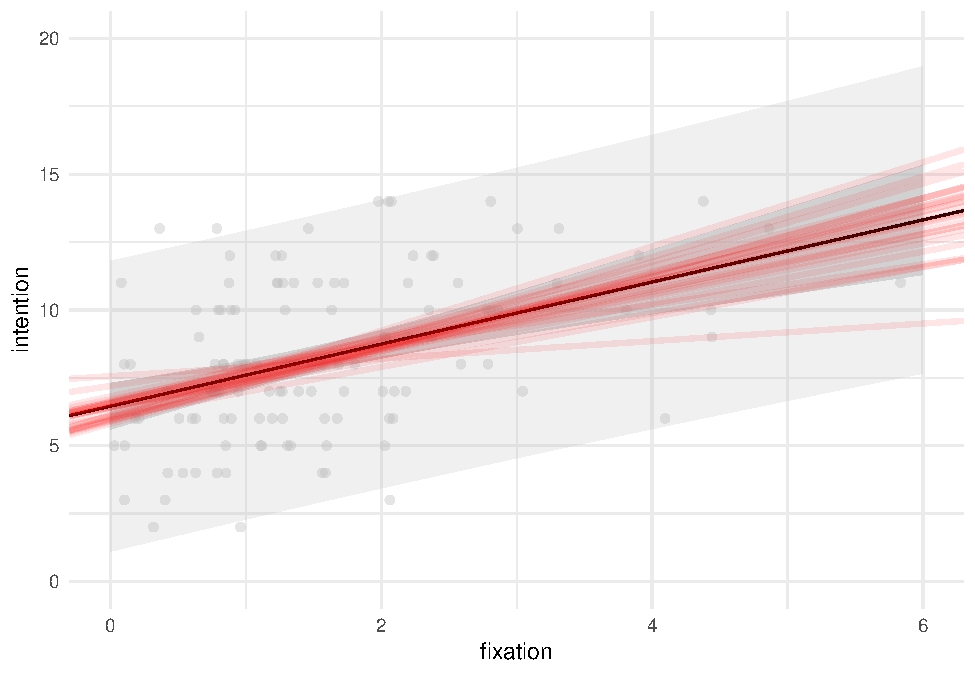
\includegraphics[width=0.7\linewidth]{MATH60604A_Statistical_modelling_files/figure-latex/predinterval-1} 

}

\caption{Prediction for the simple linear regression of buying intention as a function of fixation time. The plot shows predictions along with pointwise 95\% confidence intervals of the mean and the individual predictions.}\label{fig:predinterval}
\end{figure}

\hypertarget{interactions}{%
\section{Interactions}\label{interactions}}

In the interpretation of the linear model, the effect of an explanatory variable is assumed to be the same, regardless of the other explanatory variables (\emph{ceteris paribus}). To isolate the effect of \(\beta_j\), we indeed fix the value of the other explanatories and increase by one the variable \(\mathrm{X}_j\) (whenever this makes sense) to obtain the slope coefficient. However, the effect of a covariate may sometimes depend on another explanatory.

A good example of interaction is provided by the \texttt{insurance} dataset. An exploratory data analysis suggested that premiums depended on age, smoker status and body mass index, but through obesity status. It can be best represented graphically by looking at body mass index.

\begin{figure}

{\centering 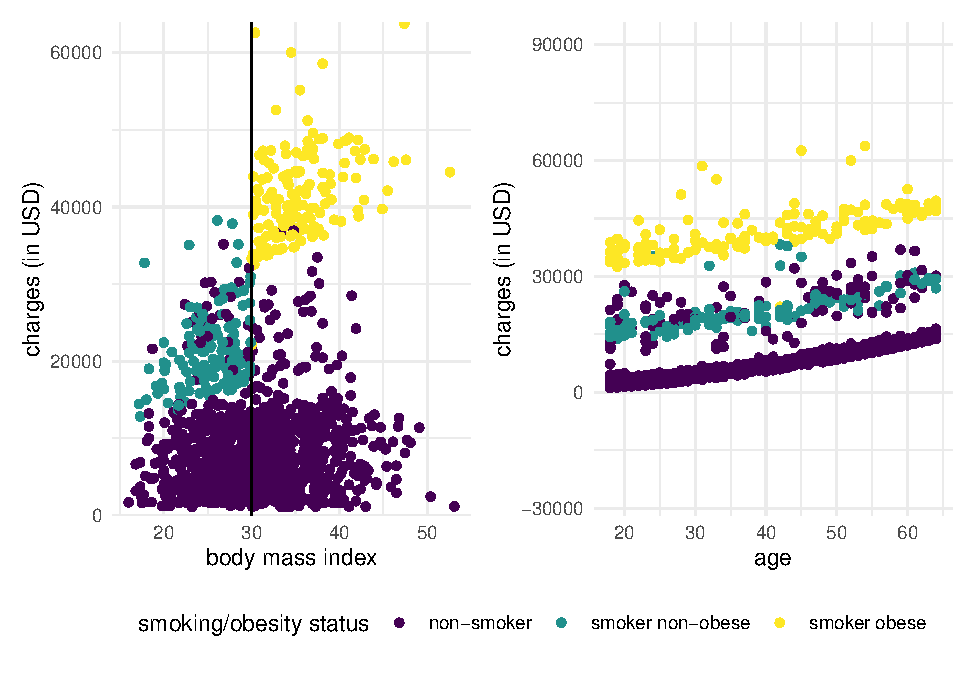
\includegraphics[width=0.7\linewidth]{MATH60604A_Statistical_modelling_files/figure-latex/insuranceinter1-1} 

}

\caption{Graph of insurance charges against body mass index. The figure clearly shows the interaction: the premium vary for smokers depending on whether or not they are obese, but we see no such behaviour for non-smokers. There is a clear linear increase of charges with age, but it is not clear whether the annual increase is the same for the three groups.}\label{fig:insuranceinter1}
\end{figure}

From there, we could create an indicator variable \(\texttt{obese}=\mathsf{I}(\texttt{bmi} \geq 30)\) and add an interaction term between smoker/obese (categorical) and age (continuous) in our mean model. We take non-smoker as baseline category. To make interpretation more meaningful, we rescale age so that \(\texttt{age}=0\) corresponds to 18 years old.

\begin{table}

\caption{\label{tab:coefintercharges}Table of regression coefficients for the insurance data with interaction terms between age, obesity and smoker status.}
\centering
\begin{tabular}[t]{lrrrr}
\toprule
term & estimate & std. error & Wald stat. & p-value\\
\midrule
(Intercept) & 2668.7 & 362.7 & 7.36 & < 0.001\\
age & 265.9 & 15 & 17.7 & < 0.001\\
obesity [obese] & 115.3 & 510.3 & 0.23 & 0.82\\
smoker [yes] & 13526.2 & 803.1 & 16.84 & < 0.001\\
age * obesity [obese] & 1.4 & 20.1 & 0.07 & 0.94\\
\addlinespace
age * smoker [yes] & -5.3 & 33.5 & -0.16 & 0.87\\
obesity [obese] * smoker [yes] & 19308.7 & 1110.5 & 17.39 & < 0.001\\
age * obesity [obese] * smoker [yes] & 19.1 & 44.8 & 0.43 & 0.67\\
\bottomrule
\end{tabular}
\end{table}

The linear regression model has eight parameters, which could be mapped to four intercepts and four different slopes for \texttt{age}; however, the model is parametrized in terms of contrasts, which facilitates testing restrictions.

\begin{align*}
\texttt{charges} &= \beta_{0} + \beta_{1}\texttt{age} + \beta_{2}\texttt{obese} + \beta_{3}\texttt{smoker} + 
\beta_{4}\texttt{age} \cdot \texttt{obese} \\&\quad + \beta_{5}\texttt{age} \cdot \texttt{smoker} + \beta_{6}\texttt{obese} \cdot \texttt{smoker} + \beta_{7}\texttt{age} \cdot \texttt{obese} \cdot \texttt{smoker} + \varepsilon
\end{align*}

Because of the three-way interaction, it is not possible to recover individual parameters by changing the value of the corresponding covariate and keeping everything else constant: changing the smoker status likely impacts multiple regressors simultaneously. To retrieve the interpretation of the different coefficients, we will need to change one parameter at the time, write the mean equation and then isolate the coefficients. Throughout, \(\texttt{obese}\) is a dummy variable equal to one if the person has a body mass index greater than 30 and likewise \(\texttt{smoker}\) if the person is a smoker.

\begin{align*}
\texttt{charges}  = 
\begin{cases}
\beta_{0} + \beta_{1}\texttt{age}  & (\mathrm{g}_1)\, \texttt{non-obese}, \texttt{non-smoker} \\
(\beta_{0} + \beta_{2}) + (\beta_{1} + \beta_{4})\texttt{age},  & (\mathrm{g}_2)\,  \texttt{obese}, \texttt{non-smoker} \\
(\beta_{0} + \beta_{3}) + (\beta_{1} + \beta_{5})\texttt{age},  & (\mathrm{g}_3)\,  \texttt{non-obese}, \texttt{smoker} \\
(\beta_{0} + \beta_{2} + \beta_{3}+ \beta_{6}) + (\beta_{1} + \beta_{4} +\beta_{5} + \beta_7)\texttt{age},  & (\mathrm{g}_4)\,  \texttt{obese}, \texttt{smoker}
\end{cases}
\end{align*}

\begin{itemize}
\tightlist
\item
  The intercept \(\beta_0\) is the average at 18 years old of non-smokers who are not obese.
\item
  The slope \(\beta_1\) is the average annual increase in charges for non-smokers who are not obese.
\item
  The parameter \(\beta_2\) is a contrast, the difference between the average charges of 18 years old non-smokers who are obese and those who are not.
\item
  The parameter \(\beta_3\) is a contrast, the difference between the average premium for non-obese 18 years old who smoke and those who don't.
\item
  The parameter \(\beta_4\) is a contrast, the difference in average annual increase for non-smokers between obese and non-obese adults.
\item
  The parameter \(\beta_5\) is a contrast, the difference in average annual increase for non-obese between smoker and non-smoker adults.
\end{itemize}

The other two coefficients, \(\beta_6\) and \(\beta_7\) represent differences of average between groups \(\mathrm{g}_1 + \mathrm{g}_4 - \mathrm{g}_2 - \mathrm{g}_3\) for both intercepts and slopes.

The only \(F\)-test that we should consider in the analysis of variance table (containing the Type III sum of squares decomposition) is the test for the three-way interaction, which corresponds to \(\mathscr{H}_0: \beta_7=0\). The \(p\)-value against the two-sided alternative is \(0.6704\), suggesting no difference in slope. The reason why we do not consider the other tests is that they correspond to irrelevant hypotheses. For example, the test for the two-way interaction term \(\mathscr{H}_0: \beta_4=0\) associated to \(\texttt{age} \cdot \texttt{obese}\) would correspond to merging the intercepts of group \(\mathrm{g}_1\) and \(\mathrm{g}_2\). Changing the baseline category would imply that a different difference in intercept is forced to be zero.

Sometimes, however, specific hypothesis could be of interest because of the problem setting. We could perform bespoke test to check here that \(\mathscr{H}_0: \beta_2=\beta_4=0\), which consists in merging the two non-smoker categories, or even \(\mathscr{H}_0: \beta_2=\beta_4= \beta_5=\beta_7=0\), which amounts to merging non-smokers and the imposing a common slope for \(\texttt{age}\). Such tests are not directly available in the output, but we can implement them manually by fitting two models and then plug-in in the values of residual sum of squares of both model in the formula of the \(F\) statistic. Using the \(F\) null distribution, we get a \(p\)-value of 0.965. This suggests both non-smoker groups are indistinguishable and likewise that there is no evidence that slopes for \(\texttt{age}\) are not equal.

Most interactions include functions of categorical variables together with either other categorical variables (different intercepts / conditional means per subgroups) or else other. Keep in mind that the validity of our tests above depend on the model being correctly specified: there is however evidence of difference in heterogeneity between groups, with unexplained non-smoker records. Plotting the residuals from the model that includes four different intercepts and slopes for \(\texttt{age}\) for each combination of smoker/obesity status misses other features that one would capture in diagnostic plots. in particular, except for some notable outliers, there is evidence that the premiums of smokers also increase with body mass index; as evidenced by Figure \ref{fig:resod}. If we include \texttt{bmi} as additional covariate in the model in addition of \texttt{obese}, the interpretation of changes in obesity will depend on the value of \texttt{bmi} and vice-versa.

\begin{figure}

{\centering 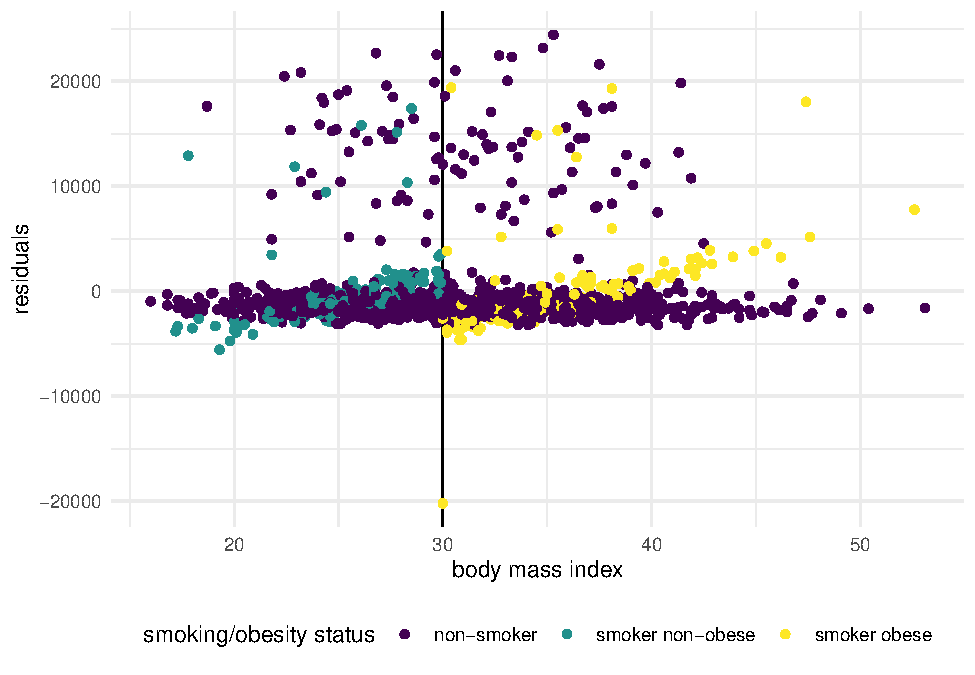
\includegraphics[width=0.7\linewidth]{MATH60604A_Statistical_modelling_files/figure-latex/resod-1} 

}

\caption{Residuals from the interaction model for $\texttt{charges}$ with $\texttt{age}$, $\texttt{smoker}$ and $\texttt{obesity}$. There is a notably outlier for a male smoker whose $\texttt{bmi}$ is exactly 30 and other points above. There is indication of a linear trend for both smoker sub-groups as their body mass index increase, which was not apparent previously because of the effect of age.}\label{fig:resod}
\end{figure}

\hypertarget{two-way-anova}{%
\subsection{Two-way ANOVA}\label{two-way-anova}}

\begin{quote}
``We're the same as regression, but we've established a separate persona.'' --- Chelsea Parlett-Pelleriti
\end{quote}

Two-way analysis of variance is a linear regression model with two categorical variables, and possibly an interaction term between the two. We consider a study on the effect of the type of delay and source of delay on the evaluation of service and on time lost waiting.

\begin{quote}
Hui, M. K., Thakor, M. V. et Gill, R. (1998). \emph{The Effects of Delay Type and Service Stage on Consumers' Reaction to Waiting}. Journal of Consumer Research \textbf{24}, 469-479.
\end{quote}

In a university, 120 participants tried a new course registration system. They were actually using a fake registration system where factors of interest could be manipulated, the advancement stage in the registration process and the type of delay. The two levels for stage of advancement were \texttt{close\ to\ end} and \texttt{far\ from\ end}. In stage \texttt{far\ from\ end}, a message indicating a delay appeared immediately at the beginning of the registration process. For the stage \texttt{close\ to\ end}, the delay message appeared after the participant has entered personal information and course choices.

There were three types of delays: \texttt{procedural}, \texttt{correctional}, and \texttt{unknown}. The delay message indicated that the server was currently busy (\texttt{procedural} delay), that there were problems with the terminal and that the system needed to reestablish the connection (\texttt{correctional} delay) or else simply stated ``please wait'' (\texttt{unknown} delay).

At the end of the registration process, the participants were asked to estimate the delay time (in minutes) incurred during the registration process. They were also asked to provide an evaluation of the service using two measurement scales. The simulated data corresponding to this study are found in the \(\texttt{delay}\) database, which contains the following variables

\begin{itemize}
\tightlist
\item
  \(\texttt{time}\): delay time (in minutes) according to the participant.
\item
  \(\texttt{eval}\): evaluation of service (standardized score).
\item
  \(\texttt{stage}\): stage of advancement, a factor with levels \texttt{close\ to\ end} and \texttt{far\ from\ end}
\item
  \(\texttt{delay}\): type of delay, a factor with levels \texttt{procedural}, \texttt{correctional} and \texttt{unknown}.
\end{itemize}

In the experimental design, the 120 participants were randomly assigned to one of these six conditions, but nine of the 120 participants were removed because they were not able to specify the type of delay that occurred. The dataset is \textbf{unbalanced}, meaning that the number of observations in each cell is unequal. If there had been the same number of observations in each subgroup for factors \(A\), \(B\), the test for the effect of factor \(A\) given that \(B\) is already in the model would be the same as the marginal effect of \(A\) only.

We will evaluate the effect of the factors \(\texttt{delay}\) and \(\texttt{stage}\) on the estimated waiting time.

If there is an interaction between explanatory variables, but the latter is not included in the models, the tests are misleading: one assumption of the linear model being that all of the relevant covariates have been included and their effect properly accounted for. In this example, omitting the interaction leads to effects being averaged and cancelling each other. Fitting an ANOVA model with only additive (main effects, without interaction) for the evaluation of service suggests that the factors \(\texttt{stage}\) and \(\texttt{delay}\) are not significant: the \(p\)-values for the main effects, reported in Table \ref{tab:summaryanovadelaynointer}, are \(0.409\) and \(0.137\). Therefore, there seemingly is no significant difference in delay time between the two stages and the three delay types.

\begin{table}

\caption{\label{tab:summaryanovadelaynointer}Analysis of variance table (Type 3 sum of square decomposition table) for the model for evaluation of service without interaction. While both factor appear not to be significant given the other, interaction plots show this is due to cancellation effects. The conclusions of the test are invalid because model assumptions are violated.}
\centering
\begin{tabular}[t]{lrrrr}
\toprule
variable & sum of square & df & F stat. & p-value\\
\midrule
(Intercept) & 0 & 1 & 0.11 & 0.74\\
stage & 0.3 & 1 & 0.69 & 0.41\\
delay & 1.6 & 2 & 2.02 & 0.14\\
Residuals & 41.9 & 105 &  & \\
\bottomrule
\end{tabular}
\end{table}

However, looking at the data and the mean of each sub-class paints a different portrait, as evidenced by the interaction plot of Figure \ref{fig:twowayanovadelay}. The score for service increases for \texttt{correctional} delays when the error occurs close to the end, but the effect is opposite for other delay types. The fact that our \(p\)-values for the effects were not significative merely indicate that the effects cancelled out each other.

\begin{figure}

{\centering 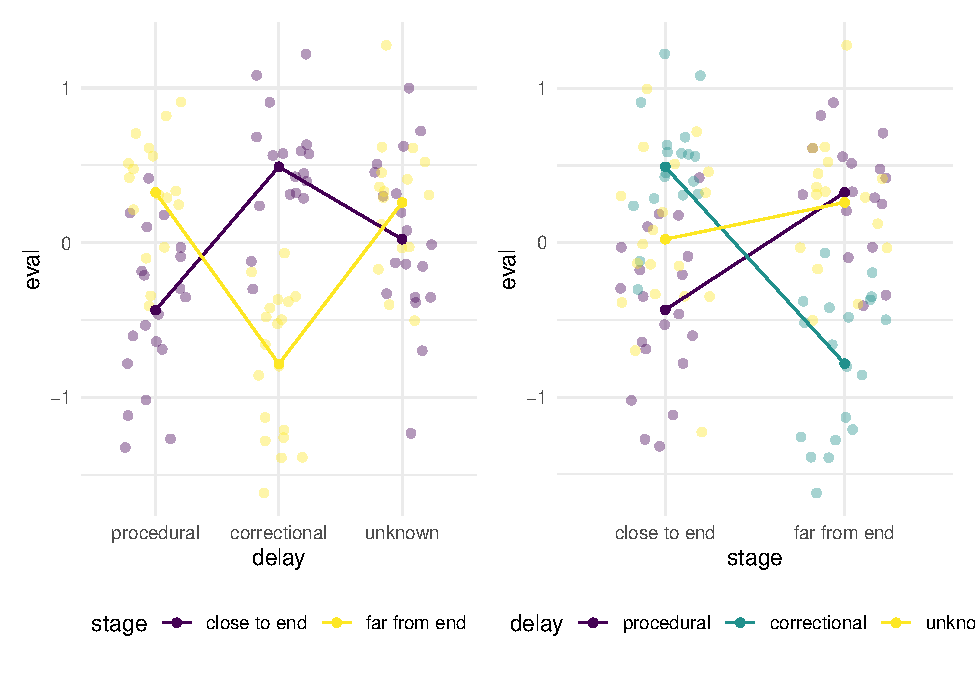
\includegraphics[width=0.7\linewidth]{MATH60604A_Statistical_modelling_files/figure-latex/twowayanovadelay-1} 

}

\caption{Interactions plots for the $\texttt{delay}$ data, with jitterd observations: if there was no interaction, the curves should be parallel. These plots seem to indicate an interaction.}\label{fig:twowayanovadelay}
\end{figure}

There is a significant interaction between the variables \(\texttt{delay}\) and \(\texttt{stage}\) on evaluation. Therefore, the effect of \(\texttt{delay}\) on the variable \(\texttt{eval}\) depends on the level of the variable \(\texttt{stage}\) ance vice-versa. Since there is an interaction term, tests for the main effects of \(\texttt{stage}\) or \(\texttt{delay}\) are not of interest.

\begin{table}

\caption{\label{tab:summarydelaywinteraction}Analysis of variance table (Type 3 sum of square decomposition table). The only test of interest is that for the interaction, which is highly significant.}
\centering
\begin{tabular}[t]{lrrrr}
\toprule
variable & sum of square & df & F stat. & p-value\\
\midrule
(Intercept) & 3.8 & 1 & 18.29 & < 0.001\\
stage & 5.3 & 1 & 25.67 & < 0.001\\
delay & 8.1 & 2 & 19.64 & < 0.001\\
stage:delay & 20.5 & 2 & 49.63 & < 0.001\\
Residuals & 21.3 & 103 &  & \\
\bottomrule
\end{tabular}
\end{table}

If a difference is detected at this stage, one could then proceed to compute all pairwise differences within a given level of the other categorical variable. This is equivalent to running multiple \(t\)-tests, but the linear model assumes equal variance and would thus pool all observations to estimate the latter. For example, we could test if the difference between procedural and correctional delays when the error occurs far from the end of the procedure is significant. The mean differences of a factor for a given level of another factor are called \textbf{simple effects}. If the interaction is significant, there must be at least one pairwise difference which is also significant. However, repeated testing can inflate the Type I error, \href{https://xkcd.com/882/}{as illustrated in this comic strip}: if we conduct 20 independent tests and the null is true in all cases (so there are no difference between any of the sub-groups), we would still expect to reject (by mistake) 1/20 on average for tests performed at level \(\alpha\). There exists method to adjust for multiple testing.

While the normality assumption is less crucial for the reliability of the tests, it requires sufficient sample size in each subgroup for these (say 20), so that the central limit theorem kicks in. The tests and models typically use the pooled variance estimators: in small samples, it makes better use of the data and has higher precision than estimators of the individual variance in each subgroups. If the variance were unequal, comparisons would require extended models covered later in the term and pairwise comparisons could be based on Welch test statistic.

\hypertarget{collinearity}{%
\section{Collinearity}\label{collinearity}}

The linearity assumption can be interpreted broadly to mean that all relevant covariates have been included and that their effect is correctly specified in the equation of the mean. Adding superfluous covariates to a model has limited impact: if the (partial) correlation between a column vector \(\mathbf{X}_k\) and the response variable \(\boldsymbol{Y}\) is zero, then \(\beta_k=0\) and the estimated coefficient \(\widehat{\beta}_k \approx 0\) because the least square estimators are unbiased. If we include many useless variables, say \(k\), the lack of parsimony can however make interpretation more difficult. The price to pay for including the \(k\) additional covariates is an increase in the variance of the estimators \(\widehat{\boldsymbol{\beta}}\).

It is nevertheless preferable to include more variables than to forget key predictors: if we omit an important predictor, their effect may be picked up by other regressors (termed \textbf{confounders}) in the model with are correlated with the omitted variable. The interpretation of the other effects can be severely affected by confounders. For example, the simple linear model (or two-sample \(t\)-test) for salary as a function of sex for the \texttt{college} data is invalid because sex is a confounder for rank. Since there are more men than women full professor, the mean salary difference between men and women is higher than it truly is. One way to account for this is to include control variables (such as rank), whose effect we need not be interested in, but that are necessary for the model to be adequate. We could also have used stratification, i.e., tested for wage discrimination within each academic rank. This is the reason why sociodemographic variables (sex, age, education level, etc.) are collected as part of studies.

A linear model is not a \href{https://xkcd.com/552/}{causal model}: all it does is capture the linear correlation between an explanatory variable and the response. When there are more than one explanatory, the effect of \(\mathrm{X}_j\) given what has not already been explained by \(\mathbf{X}_{-j}\). Thus, if we fail to reject \(\mathscr{H}_0:\beta_j=0\) in favor of the alternative \(\mathscr{H}_1: \beta_j \neq 0\), we can only say that there is no significant \emph{linear} association between \(\mathrm{X}_j\) and \(Y\) once the effect of other variables included in the model has been accounted for. There are thus two scenarios: either the response is uncorrelated with \(\mathrm{X}_j\) (uninteresting case, but easy to pick up by plotting both or computing linear correlation), or else there is a strong correlation between \(\mathrm{X}_j\) and both the response \(Y\) as well as (some) of the other explanatory variables \(\mathrm{X}_1, \ldots, \mathrm{X}_p\). This problem is termed (multi)collinearity.

One potential harm of collinearity is a decrease in the precision of parameter estimators. With collinear explanatories, many linear combinations of the covariates represent the response nearly as well. Due to the (near) lack of identifiability, the estimated coefficients become numerically unstable and this causes an increase of the standard errors of the parameters. The predicted or fitted values are unaffected. Generally, collinearity leads to high estimated standard errors and the regression coefficients can change drastically when new observations are included in the model, or when we include or remove explanatories. The individual \(\beta\) coefficients may not be statistically significant, but the global \(F\)-test will indicate that some covariates are relevant for explaining the response. This however would also be the case if there are predictors with strong signal, so neither is likely to be useful to detect issues.

The added-variable plot shows the relation between the response \(Y\) and an explanatory \(\mathrm{X}_j\) after accounting for other variables: the slope \(\widehat{\beta}_j\) of the simple linear regression is the same of the full model. A similar idea can be used to see how much of \(\mathrm{X}_j\) is already explained by the other variables. For a given explanatory variable \(\mathrm{X}_j\), we define its \textbf{variance inflation factor} as \(\mathsf{VIF}(j)=(1-R^2(j))^{-1}\), where \(R^2(j)\) is the coefficient of determination of the model obtained by regressing \(\mathrm{X}_j\) on all the other explanatory variables, i.e.,
\begin{align*}
\mathrm{X}_j = \beta^{\star}_0 + \beta^{\star}_1 \mathrm{X}_1 + \cdots + \beta^{\star}_{j-1} \mathrm{X}_{j-1} + \beta^{\star}_{j+1} \mathrm{X}_{j+1} + \cdots + \beta^{\star}_p\mathrm{X}_p + \varepsilon^{\star}
\end{align*}
By definition, \(R^2(j)\) represents the proportion of the variance of \(\mathrm{X}_j\) that is explained by all the other predictor variables. Large variance inflation factors are indicative of problems (typically covariates with \(\mathsf{VIF}>10\) require scrutinity, and values in the hundreds or more indicate serious problems).

Added-variable plots can also serve as diagnostics, by means of comparison of the partial residuals with a scatterplot of the pair \((Y, \mathrm{X}_j)\); if the latter shows very strong linear relation, but the slope is nearly zero in the added-variable plot, this hints that collinearity is an issue.

What can one do about collinearity? If the goal of the study is to develop a predictive model and we're not interested in the parameters themselves, then we don't need to do anything. Collinearity is not a problem for the overall model: it's only a problem for the individual effects of the variables. Their joint effect is still present in the model, regardless of how the individual effects are combined.

If we are interested in individual parameter estimates, for example,
to see how (and to what extent) the predictor variables explain the behaviour of \(Y\), then things get more complicated. Collinearity only affects the variables that are strongly correlated with one another, so we only care if it affects one or more of the variables of interest. There sadly is no good solution to the problem. One could

\begin{itemize}
\tightlist
\item
  try to obtain more data, so as to reduce the effects of collinearity appearing in specific samples or that are due to small sample size.
\item
  create a composite score by somehow combining the variables showing collinearity.
\item
  remove one or more of the collinear variables. You need to be careful when doing this not to end up with a misspecified model.
\item
  use penalized regression. If \(\mathbf{X}^\top\mathbf{X}\) is (nearly) not invertible, this may restore the uniqueness of the solution. Penalties introduce bias, but can reduce the variance of the estimators \(\boldsymbol{\beta}\). Popular choices include ridge regression (with an \(l_2\) penalty), lasso (\(l_1\) penalty), but these require adjustment in order to get valid inference.
\end{itemize}

Whatever the method, it's important to understand that it can be very difficult (and sometimes impossible) to isolate the individual effect of a predictor variable strongly correlated with other predictors.

\begin{example}[Collinearity in the $\texttt{college}$ data]
\protect\hypertarget{exm:collegedatcollinear}{}{\label{exm:collegedatcollinear} \iffalse (Collinearity in the \(\texttt{college}\) data) \fi{} }We consider the \texttt{college} data analysis and include all the covariates in the database, including \texttt{years}, the number of years since PhD. One can suspect that, unless a professor started his or her career elsewhere before moving to the college, they will have nearly the same years of service. In fact, the correlation between the two variables, \texttt{service} and \texttt{years} is \texttt{r\ cor(college\$service,\ college\$years)}. The variance inflation factor for the five covariates

For categorical variables, the variance inflation factor definition would normally yield for each level a different value; an alternative is the generalized variance inflation factor \citep{Fox:1992}. Here, we are interested in gender disparities, so the fact that both service and field are
strongly correlated is not problematic, since the \(\mathsf{VIF}\) for \(\texttt{sex}\) is not high and the other variables are there to act as control and avoid confounders.
\end{example}

\begin{table}

\caption{\label{tab:unnamed-chunk-1}(Generalized) variance inflation factor for the $\texttt{college}$ data.}
\centering
\begin{tabular}[t]{rrrrr}
\toprule
service & years & rank & sex & field\\
\midrule
5.92 & 7.52 & 2.01 & 1.03 & 1.06\\
\bottomrule
\end{tabular}
\end{table}

\hypertarget{graphical-analysis-of-residuals}{%
\section{Graphical analysis of residuals}\label{graphical-analysis-of-residuals}}

So far, we have fit models and tested significance of the parameters without checking the model assumptions. The correctness of statements about the \(p\)-values and confidence intervals depend on the (approximate) validity of the model assumptions, which all stem from the distributional assumption for the error, assumed to be independent and identically distributed with \(\varepsilon_i \stackrel{\cdot}{\sim} \mathsf{No}(0, \sigma^2)\). This compact mathematical description can be broken down into four assumptions.

\begin{itemize}
\tightlist
\item
  normality of the errors
\item
  linearity: the mean of \(Y\) is \(\beta_0 + \beta_1\mathrm{X}_1 + \cdots + \beta_p \mathrm{X}_p\).
\item
  homoscedasticity: the error variance is constant
\item
  independence of the errors.
\end{itemize}

This section reviews the assumptions made in order to allow statistical inference using the linear model and different residuals that serve as building blocks for graphical diagnostics. We investigate the consequences of violation of these assumptions and outline potential mitigation strategies, many of which are undertaken in other chapters.

When we perform an hypothesis test, we merely fail to reject the null hypothesis, either because the latter is true or else due to lack of evidence. The same goes for checking the validity of model assumptions: scientific reasoning dictates that we cannot know for certain whether these hold true. Our strategy is therefore to use implications of the linear model assumptions to create graphical diagnostic tools, so as to ensure that there is no gross violation of these hypothesis. However, it is important to beware of over-interpreting diagnostic plots: the human eye is very good at finding spurious patterns.

Other good references for the material in this section is:

\begin{itemize}
\tightlist
\item
  \href{https://otexts.com/fpp2/regression-evaluation.html}{Forecasting: Principles and Practice, section 5.3}
\end{itemize}

\hypertarget{residuals}{%
\subsection{Residuals}\label{residuals}}

Residuals are predictions of the errors \(\varepsilon\) and represent the difference between the observed value \(Y_i\) and the estimated value on the line.
The ordinary residuals are
\begin{align*}
e_i=Y_i-\widehat{Y}_i, \qquad i =1, \ldots, n.
\end{align*}
The sum of the ordinary residuals is always zero by construction if the model includes an intercept, meaning \(\overline{e} = 0\).

Not all observations contribute equally to the adjustment of the fitted hyperplane. The geometry of least squares shows that the residuals are orthogonal to the fitted values, and \(\boldsymbol{e} = (\mathbf{I}_n-\mathbf{H}_{\mathbf{X}})\boldsymbol{Y}\), where \(\mathbf{H}_{\mathbf{X}}=\mathbf{X}(\mathbf{X}^\top\mathbf{X})^{-1}\mathbf{X}^\top\) is an \(n \times n\) projection matrix that spans the \(p\)-dimensional linear combination of the columns of \(\mathbf{X}\), \(\mathcal{S}(\mathbf{X})\). If \(\mathsf{Va}(\boldsymbol{Y}) = \sigma^2\mathbf{I}_n\), it follows that \(\mathsf{Va}(\boldsymbol{e})=\sigma^2(\mathbf{I}_n-\mathbf{H}_{\mathbf{X}})\) because \((\mathbf{I}_n-\mathbf{H}_{\mathbf{X}})\) is a projection matrix, therefore idempotent and symmetric. Because the matrix has rank \(n-p\), the ordinary residuals cannot be independent from one another.

If the errors are independent and homoscedastic, the ordinary residual \(e_i\) has variance \(\sigma^2(1-h_{i})\), where the leverage term \(h_i =(\mathbf{H}_{\mathbf{X}})_{ii} = \mathbf{x}_i (\mathbf{X}^\top\mathbf{X})^{-1}\mathbf{x}_i\) is the \(i\)th diagonal entry of the projection matrix \((\mathbf{H}_{\mathbf{X}})\) and \(\mathbf{x}_i\) is the \(i\)th row of the model matrix corresponding to observation \(i\).

We thus conclude that ordinary residuals do not all have the same standard deviation and they are not independent. This is problematic, as we cannot make meaningful comparisons: points with low leverage are bound to deviate more from the fitted model than others. To palliate to this, we can standardize the residuals so each has the same variance under the null of independent homoscedastic errors --- the leverage terms \(h_i\) are readily calculated from the model matrix \(\mathbf{X}\).
The only remaining question is how to estimate the variance. If we use the \(i\)th observation to estimate both the residual and the variance, we introduce additional dependence. A better way is remove the \(i\)th observation and refit the model with the \(n-1\) remaining observations to get of \(s^2_{(-i)}\) (there are tricks and closed-form expressions for these, so one doesn't need to fit \(n\) different linear models). The jacknife studentized residual \(r_i = e_i/\{s_{(-i)}(1-h_i)\}\), also termed externally studentized residuals, are not independent, but they are identically distributed and follow a Student distribution with \(n-p-2\) degrees of freedom.
These can be obtained in \textbf{R} with the command \texttt{rstudent}, also in \textbf{SAS}.

When to use which residuals? By construction, the vector of ordinary residuals \(\boldsymbol{e}\) is orthogonal to the fitted values \(\widehat{\boldsymbol{y}}\) and also to each column of the model matrix \(\mathbf{X}\): this means a simple linear regression of \(\boldsymbol{e}\) with any of these as covariate gives zero intercept and zero slope. However, residual patterns due to forgotten interactions, nonlinear terms, etc. could be picked up from pair plots of ordinary residuals against the explanatories.

While the jackknife studentized residuals \(r_i\) are not orthogonal, they are not very different. Use jackknife residuals \(\boldsymbol{r}\) to check for equality of variance and distributional assumptions (e.g., using quantile-quantile plots).

One thus typically uses ordinary residuals \(\boldsymbol{e}\) for plots of fitted values/explanatories against residuals and otherwise jackknife studentized residuals for any other graphical diagnostic plot.

\hypertarget{leverage-and-outliers}{%
\subsection{Leverage and outliers}\label{leverage-and-outliers}}

The leverage \(h_i\) of observation \(i\) measures its impact on the least square fit, since we can write \(h_i = \partial \widehat{y}_i/\partial y_i\). Leverage values tell us how much each point impacts the fit: they are strictly positive, are bounded below by \(1/n\) and above by \(1\). The sum of the leverage values is \(\sum_{i=1}^n h_i=p+1\): in a good design, each point has approximately the same contribution, with average weight \((p+1)/n\).

Points with high leverage are those that have unusual combinations of explanatories. An influential observation (\(h_i\approx 1\)) pulls the fitted hyperplane towards itself so that \(\hat{y}_i \approx y_i\). As a rule of thumb, points with \(h_i> 2(p+1)/n\) should be scrutinized.

It is important to distinguish betwen \textbf{influential} observations (which have unusual \(\mathbf{x}\) value, i.e., far from the overall mean) and \textbf{outliers} (unusual value of the response \(y\)).
If an observation is both an outlier and has a high leverage, it is problematic.

\begin{figure}

{\centering 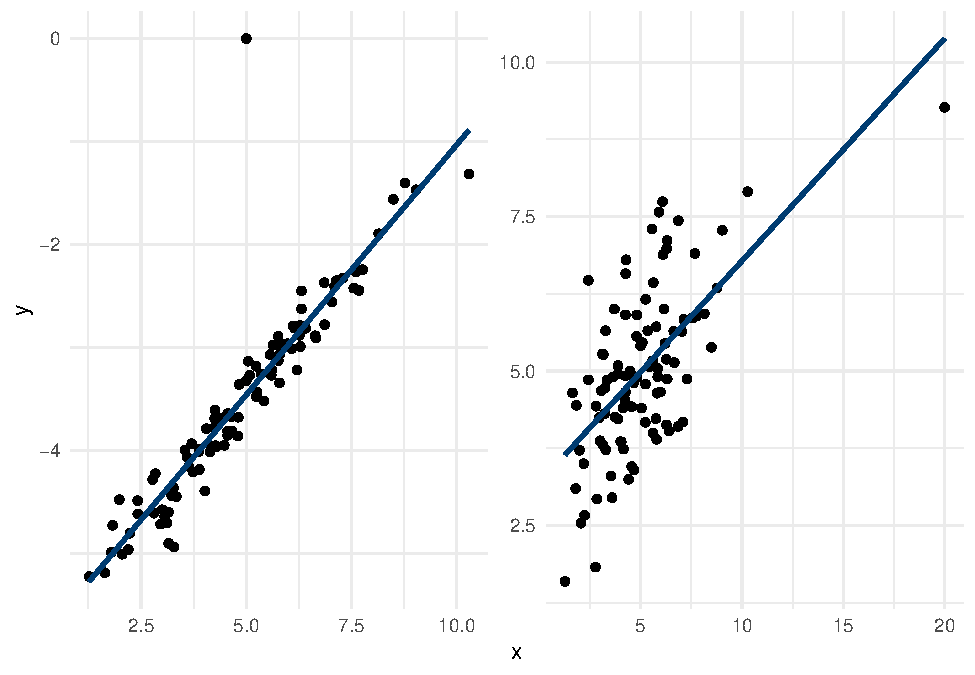
\includegraphics[width=0.7\linewidth]{MATH60604A_Statistical_modelling_files/figure-latex/outliers-1} 

}

\caption{Outlier and influential observation. The left panel shows an outlier, whereas the right panel shows an influential variable (rightmost $x$ value).}\label{fig:outliers}
\end{figure}

If influential observations can be detected by inspecting the leverage of each observation, outliers are more difficult to diagnose.

An outlier stands out from the rest of the observations, either because it has an usual response value, or because it falls far from the regression surface.
Loosely speaking, an outlier is an unusual values of \(Y\) for a given combination of \(\mathbf{X}\) that ``stand out'\,' from the rest.
Outliers can be detected during the exploratory data analysis or picked-up in residual plots (large values of \(|e_i|\) in plots of fitted versus residuals) or added-variable plots. One could potentially test whether an jackknife studentized residual is an outlier (adjusting for the fact we would consider only largest values). One can also consider Cook's distance, \(C_j\), a statistic giving the scaled distance between the fitted values \(\hat{\boldsymbol{y}}\) and the fitted values for the model with all but the \(j\)th observation, \(\hat{\boldsymbol{y}}^{(-j)}\),
\begin{align*}
C_j = \frac{1}{(p+1)S^2} \sum_{i=1}^n \left\{\hat{y}_i - \hat{y}_{i}^{(-j)}\right\}^2
\end{align*}
Large values of \(C_j\) indicate that its residual \(e_j\) is large relative to other observations or else its leverage \(h_j\) is high. A rule of thumb is to consider points for which \(C_j > 4/(n-p-1)\). In practice, if two observations are outlying and lie in the same region, their Cook distance will be halved.

Outliers and influential observations should not be disregarded because they don't comply with the model, but require further investigation. They may motivate further modelling for features not accounted for. It is also useful to check for registration errors in the data (which can be safely discarded).

Except in obvious scenarios, unusual observations should not be discarded. In very large samples, the impact of a single outlier is hopefully limited. Transformations of the response may help reduce outlyingness. Otherwise, alternative objective functions (as those employed in robust regression) can be used; these downweight extreme observations, at the cost of efficiency.

\hypertarget{diagnostic-plots}{%
\subsection{Diagnostic plots}\label{diagnostic-plots}}

We review the assumptions in turn and discuss what happens when the assumptions fail to hold.

\hypertarget{independence-assumption}{%
\subsubsection{Independence assumption}\label{independence-assumption}}

Usually, the independence of the observations follows directly from the type of sampling used --- this assumption is implicitly true if the observations were taken from a \emph{random sample} from the population. This is generally not the case for longitudinal data, which contains repeated measures from the same individuals across time. Likewise, time series are bound not to have independent observations. If we want to include all the time points in the analysis, we must take into account the possible dependence (correlation) between observations. If we ignore correlation, the estimated standard errors are too small relative to the truth, so the effective sample size is smaller than number of observations.

The first source of dependence is clustered data, meaning measurements taken from subjects that are not independent from one another (family, groups, etc.)
More generally, correlation between observations arises from time dependence, roughly categorized into

\begin{itemize}
\tightlist
\item
  longitudinal data: repeated measurements are taken from the same subjects (few time points)
\item
  time series: observations observed at multiple time periods (many time points). Time series require dedicated models not covered in this course.
\end{itemize}

Because of autocorrelation, positive errors tend to be followed by positive errors, etc. We can plot the residuals as a function of time, and a scatterplot of lagged residuals \(e_i\) versus \(e_{i-1}\) (\(i=2, \ldots, n\)).

\begin{figure}

{\centering 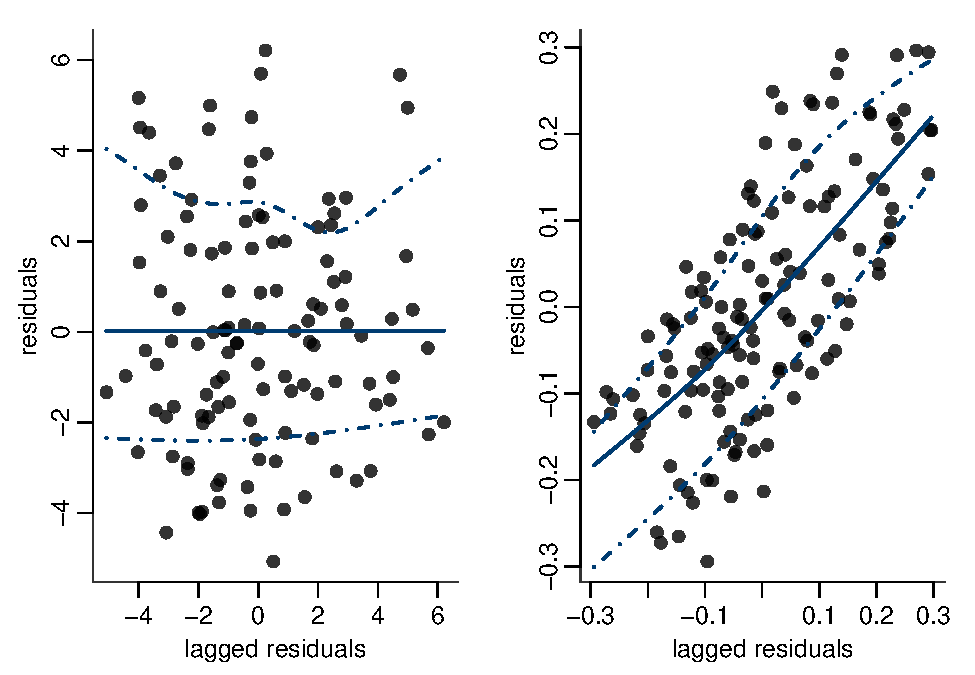
\includegraphics[width=0.7\linewidth]{MATH60604A_Statistical_modelling_files/figure-latex/timeresidplot-1} 

}

\caption{Lagged residual plots: there is no evidence against independence in the left panel, whereas the right panel shows positively correlated residuals.}\label{fig:timeresidplot}
\end{figure}

However, lagged residuals plots only show dependence at lag one between observations. For time series, we can look instead at a correlogram, i.e., a bar plot of the correlation between two observations \(h\) units apart as a function of the lag \(h\) \citep[Definition 1.4.4]{Brockwell/Davis:2016}.

For \(y_1, \ldots, y_n\) and constant time lags \(h=0, 1, \ldots\) units, the autocorrelation at lag \(h\) is
\begin{align*}
r(h) = \frac{\gamma(h)}{\gamma(0)}, \qquad \gamma(h) = \frac{1}{n}\sum_{i=1}^{n-|h|} (y_i-\overline{y})(y_{i+h}) - \overline{y}) 
\end{align*}

If the series is correlated, the sample autocorrelation will likely fall outside of the pointwise confidence intervals, as shown in Figure \ref{fig:correlogram}. Presence of autocorrelation requires modelling the correlation between observations explicitly using dedicated tools from the time series literature that are covered in MATH 60638. We will however examine \(\mathsf{AR}(1)\) models as part of the chapter on longitudinal data.

When observations are positively correlated, the estimated standard errors reported by the software are too small. This means we are overconfident and will reject the null hypothesis more often then we should if the null is true (inflated Type I error, or false positive).

\begin{figure}

{\centering 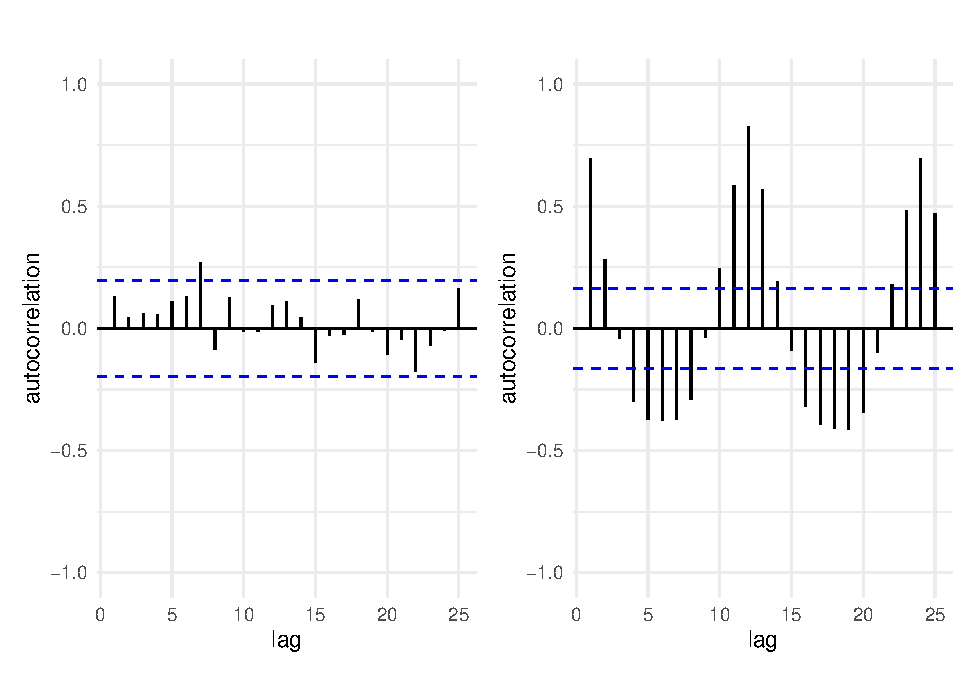
\includegraphics[width=0.7\linewidth]{MATH60604A_Statistical_modelling_files/figure-latex/correlogram-1} 

}

\caption{Correlogram of independent observations (left) and the ordinary residuals of the log-linear model fitted to the air passengers data (right). While the mean model of the latter is seemingly correctly specified, there is residual dependence between monthly observations and yearly (at lag 12). The blue lines give approximate pointwise 95\% confidence intervals for white noise (uncorrelated observations).}\label{fig:correlogram}
\end{figure}

\hypertarget{linearity-assumption}{%
\subsubsection{Linearity assumption}\label{linearity-assumption}}

The second assumption of the linear model is that of linearity, which means that the mean model is correctly specified, all relevant covariates have been included and their effect is correctly specified.
To check that the response surface of the linear model is adequate, we plot \(e_i\) against \(\widehat{y}_i\) or \(\mathrm{X}_{ij}\) (for \(j=1, \ldots, p\)). Since the linear correlation between \(\boldsymbol{e}\) and \(\widehat{\boldsymbol{y}}\) (or \(\boldsymbol{e}\) and \(\mathbf{X}_j\)) is zero by construction, patterns (e.g., quadratic trend, cycles, changepoints) are indicative of misspecification of the mean model. One can add a smoother to detect patterns. Figure \ref{fig:regdiaglin} shows three diagnostics plots, the second of which shows no pattern in the residuals, but skewed fitted values.

\begin{figure}

{\centering 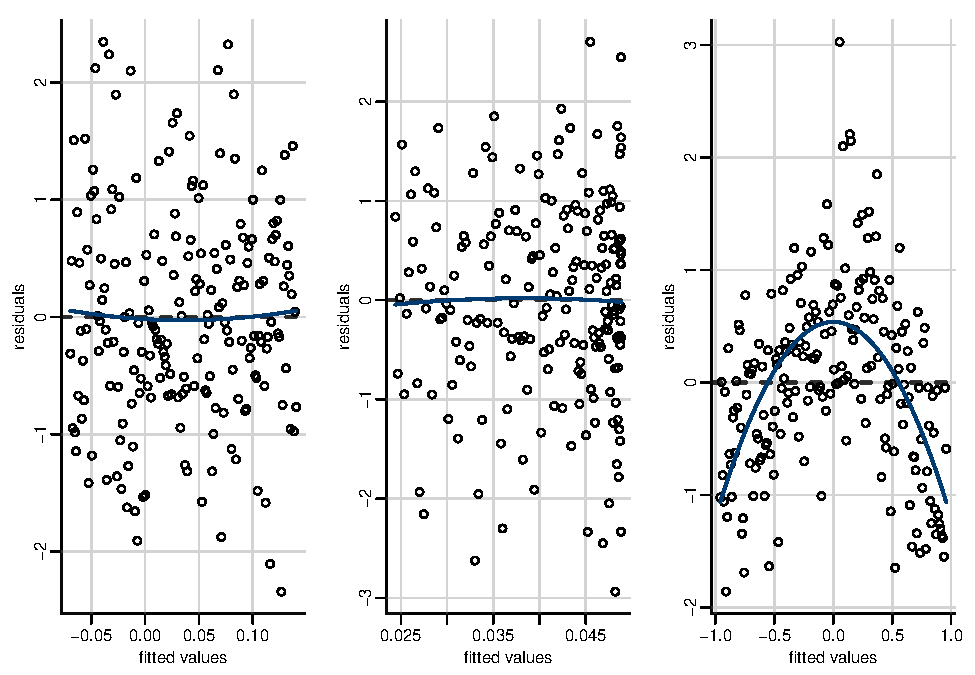
\includegraphics[width=0.7\linewidth]{MATH60604A_Statistical_modelling_files/figure-latex/regdiaglin-1} 

}

\caption{Scatterplots of residuals against fitted values. The first two plots show no departure from linearity (mean zero). The third plot shows a clear quadratic pattern, suggesting the mean model is misspecified. Note that the distribution of the fitted value need not be uniform, as in the second panel which shows more high fitted values.}\label{fig:regdiaglin}
\end{figure}

If there is residual structure in plots of ordinary residuals against either (a) the fitted values or (b) the explanatory variables, a more complex model can be adjusted including interactions, nonlinear functions, \ldots If the effect of an explanatory variable is clearly nonlinear and complicated, smooth terms could be added (we won't cover generalized additive models in this course).

Plotting residuals against left-out explanatory variables can also serve to check that all of the explanatory power of the omitted covariate is already explained by the columns of \(\mathbf{X}\).

If an important variable has been omitted and is not available in the dataset, then the effect of that variable is captured by both the errors (the portion orthogonal to the model matrix \(\mathbf{X}\), i.e., unexplained by the covariates included in the model) and the remaining part is captured by other explanatories of the model that are correlated with the omitted variable. These variables can act as confounders. There is little that can be done in either case unless the data for the omitted variable are available, but subject-specific knowledge may help make sense of the results.

\hypertarget{homoscedasticity-assumption}{%
\subsubsection{Homoscedasticity assumption}\label{homoscedasticity-assumption}}

If the variance of the errors is the same for all observations, that of the observations \(Y\) is also constant. The most common scenarios for heteroscedasticity are increases in variance with the response, or else variance that depends on explanatory variables \(\mathbf{X}\), most notably categorical variables. For the former, a log-transform (or Box--Cox transformation) can help stabilize the variance, but we need the response to be positive. For the latter, we can explicitly model that variance and we will see how to include different variance per group later on. A popular strategy in the econometrics literature, is to use robust (inflated) estimators of the standard errors such as \href{https://en.wikipedia.org/wiki/Heteroscedasticity-consistent_standard_errors}{White's sandwich estimator of the variance}.

If the residuals (or observations) are heteroscedastic (non constant variance), the estimated effects of the variables (the \(\beta\) parameters) are still valid in the sense that the ordinary least squares estimator \(\widehat{\boldsymbol{\beta}}\) is unbiased. However, the estimated standard errors of the \(\widehat{\beta}\) are no longer reliable and, consequently, the confidence intervals and the hypothesis tests for the model parameters will be incorrect. Indeed, if the variance of the errors differs from one observation to the next, we will estimate an average of the different variance terms. The standard errors of each term are incorrect (too small or too large) and the conclusions of the tests (\(p\)-values) will be off because the formulas of both \(t\)-test and \(F\)-test statistics include estimates of \(\hat{\sigma}^2\).

Looking at the plot of jackknife studentized residuals against regressors (or fitted values) is instructive --- for example, we often see a funnel pattern when there is an increase in variance in the plot of the jackknife studentized residuals against fitted value, or else in boxplots with a categorical variable as in Figure \ref{fig:diagfitvalhomosce}.
However, if we want to fit a local smoother to observe trends, it is better to plot the absolute value of the jackknife studentized residuals against regressors or observation number.

\begin{figure}

{\centering 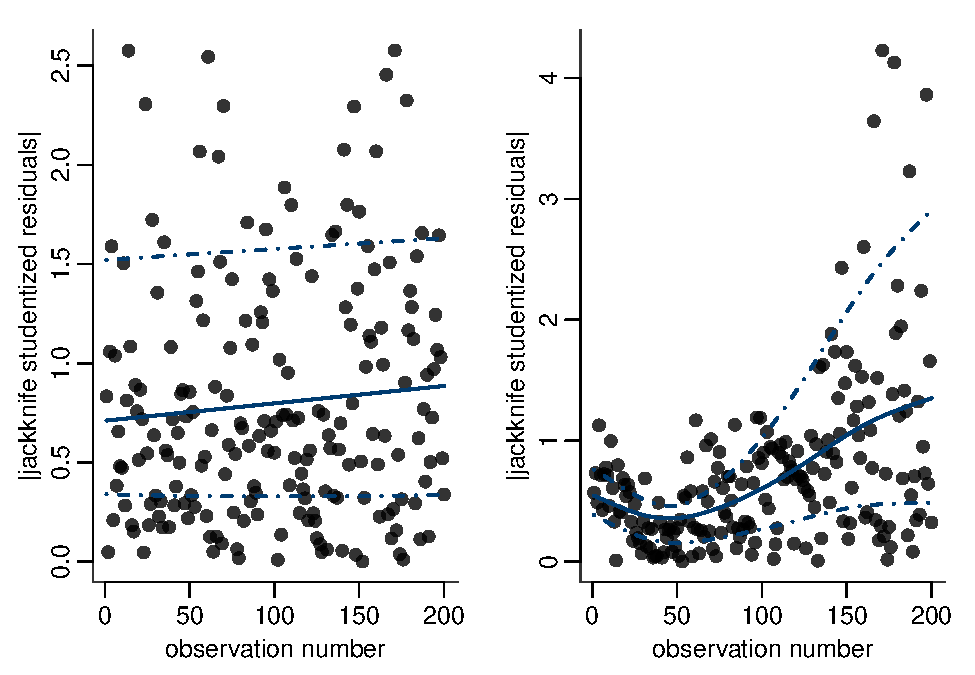
\includegraphics[width=0.7\linewidth]{MATH60604A_Statistical_modelling_files/figure-latex/residhomoscedastic-1} 

}

\caption{Plot of the absolute value of jackknife studentized residuals against observation number. The left panel is typical of homoscedastic data, whereas the right panel indicates an increase in the variance.}\label{fig:residhomoscedastic}
\end{figure}

\begin{figure}

{\centering 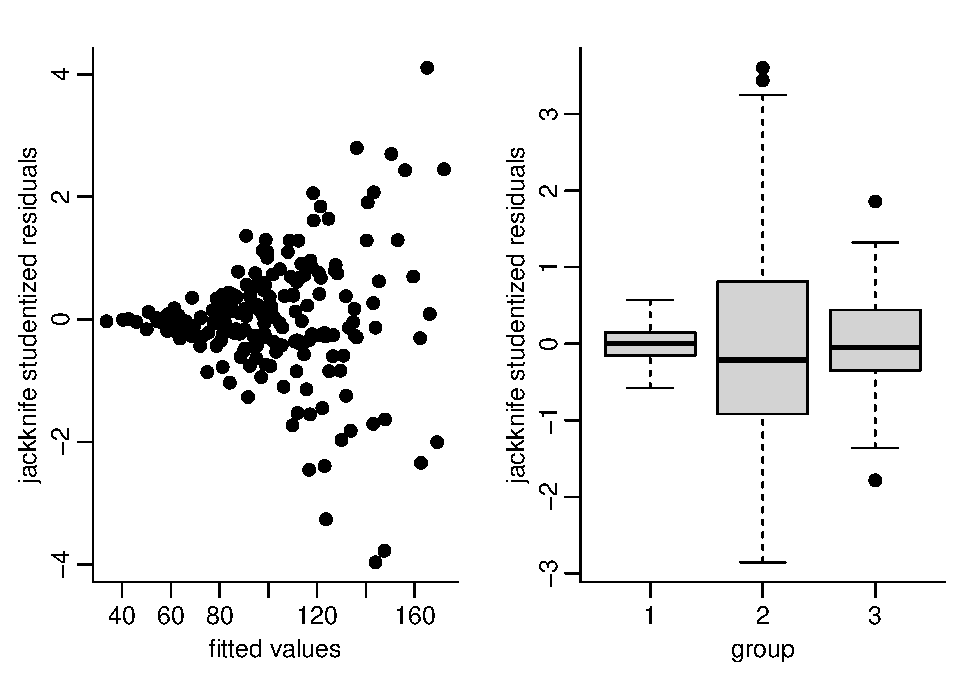
\includegraphics[width=0.7\linewidth]{MATH60604A_Statistical_modelling_files/figure-latex/diagfitvalhomosce-1} 

}

\caption{Plot of jackknife studentized residuals against fitted value (left) and categorical explanatory (right). Both clearly display heteroscedasticity.}\label{fig:diagfitvalhomosce}
\end{figure}

\hypertarget{normality-assumption}{%
\subsubsection{Normality assumption}\label{normality-assumption}}

The normality assumption is mostly for convenience: if the errors are assumed normally distributed, then the least square and the maximum likelihood estimators of \(\boldsymbol{\beta}\) coincide.
The maximum likelihood estimators of \(\boldsymbol{\beta}\) are asymptotically normal under mild conditions on the model matrix and \(t\)-tests are robust to departure of the normality assumption. This means that inference is valid in large samples, regardless of the distribution of the errors/residuals (even if the null distribution are not exact). It is important to keep in mind that, for categorical explanatory variables, the sample size in each group must be sufficiently large for the central limit theorem to kick in.

Sometimes, transformations can improve normality: if the data is right-skewed and the response is strictly positive, a log-linear model may be more adequate. This can be assessed by looking at the quantile-quantile plot of the externally studentized residuals. If the response \(Y\) is not continuous (including binary, proportion or count data), linear models give misleading answers and generalized linear models are more suitable.

The inference will be valid for large samples even if the errors are not normally distributed by virtue of the central limit theorem. If the errors \(\varepsilon_i \sim \mathsf{No}(0, \sigma^2)\), then the jacknnife studentized residuals should follow a Student distribution, with \(r_i \sim \mathsf{St}(n-p-2)\), (identically distributed, but not independent). A Student quantile-quantile plot can thus be used to check the assumption (and for \(n\) large, the normal plotting positions could be used as approximation if \(n-p> 50\)). One can also plot a histogram of the residuals. Keep in mind that if the mean model is not correctly specified, some residuals may incorporate effect of leftover covariates.

\begin{figure}

{\centering 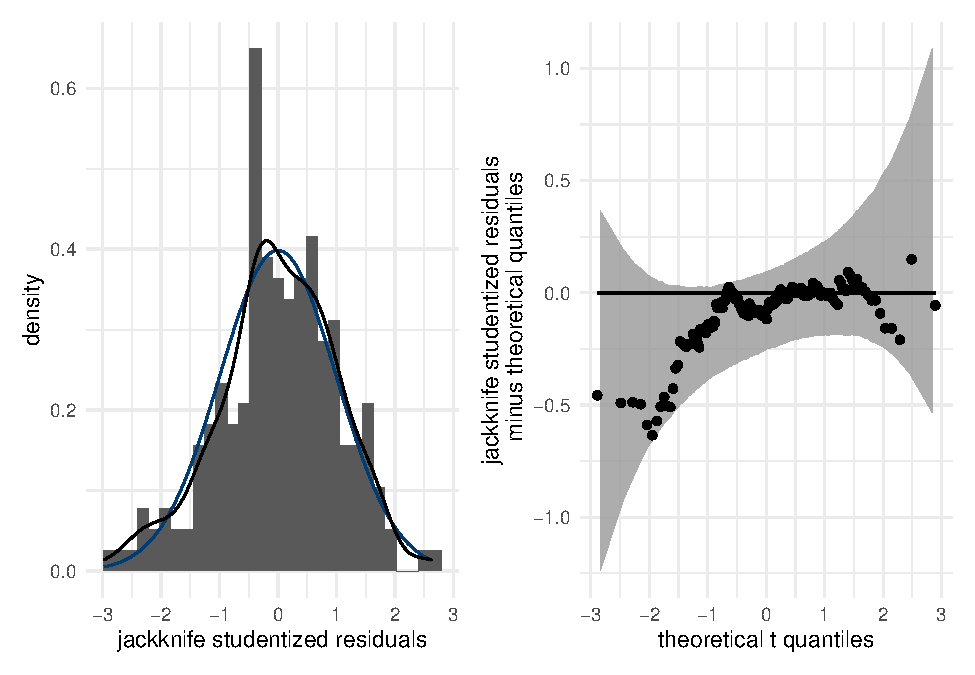
\includegraphics[width=0.7\linewidth]{MATH60604A_Statistical_modelling_files/figure-latex/qqplotresid-1} 

}

\caption{Histogram (left) and Student quantile-quantile plot (right) of the jackknife studentized residuals. The left panel includes a kernel density estimate (black), with the density of Student distribution (blue) superimposed. The right panel includes pointwise 95\% confidence bands calculated using a bootstrap.}\label{fig:qqplotresid}
\end{figure}

Quantile-quantile plots are discussed in Section \ref{diagramme-qq}, but their interpretation requires training. For example, Figure \ref{fig:qqplotsbad} shows many common scenarios that can be diagnosed using quantile-quantile plots: discrete data is responsible for staircase patterns, positively skewed data has too high low quantiles and too low high quantiles relative to the plotting positions, heavy tailed data have high observations in either tails and bimodal data leads to jumps in the plot.

\begin{figure}

{\centering 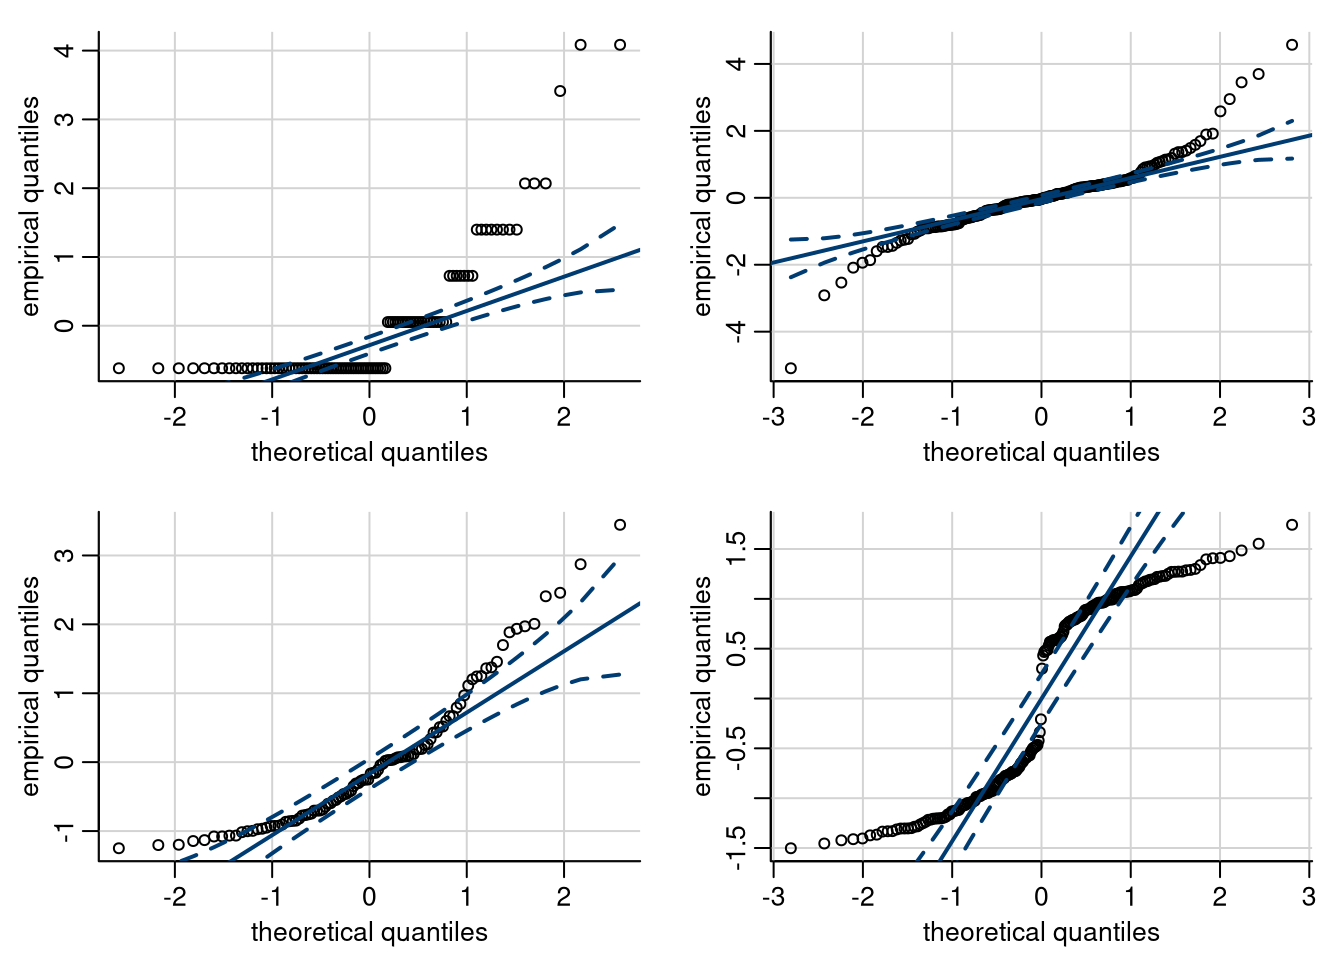
\includegraphics[width=0.7\linewidth]{MATH60604A_Statistical_modelling_files/figure-latex/qqplotsbad-1} 

}

\caption{Quantile-quantile plots of non-normal data, showing typical look of behaviour of discrete (top left), heavy tailed  (top right), skewed (bottom left) and bimodal data (bottom right).}\label{fig:qqplotsbad}
\end{figure}

\begin{example}[Diagnostic plots for the $\texttt{college}$ data.]
\protect\hypertarget{exm:diagplotcollege}{}{\label{exm:diagplotcollege} \iffalse (Diagnostic plots for the \(\texttt{college}\) data.) \fi{} }We can look at the \texttt{college} data to see if the linear model assumptions hold.
\end{example}

\begin{figure}

{\centering 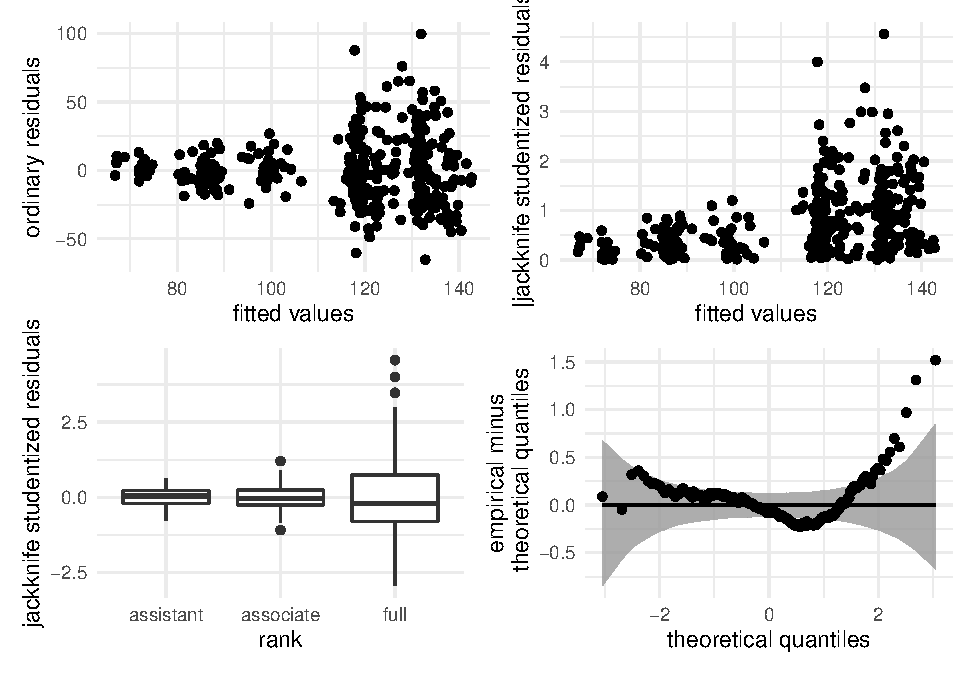
\includegraphics[width=0.7\linewidth]{MATH60604A_Statistical_modelling_files/figure-latex/diagplotscollege-1} 

}

\caption{Diagnostic plots for the college data example: ordinary residuals against fitted values (top left), absolute value of the jacknnife studentized residuals against fitted values (top right), box and whiskers plot of jacknnife studentized residuals (bottom left) and detrended Student quantile-quantile plot (bottom right). There is clear group heteroscedasticity.}\label{fig:diagplotscollege}
\end{figure}

Based on the plots of Figure \ref{fig:diagplotscollege}, we find that there is residual heteroscedasticity, due to rank. Since the number of years in the first rank is limited and all assistant professors were hired in the last six years, there is less disparity in their income. It is important not to mistake the pattern on the \(x\)-axis for the fitted value (due to the large effect of rank and field, both categorical variable) with patterns in the residuals (none apparent). Fixing the heteroscedasticity would correct the residuals and improve the appearance of the quantile-quantile plot.

\hypertarget{transformation-response}{%
\section{Transformation of the response}\label{transformation-response}}

This ultimate section deals with strategies for fixing the linear model if we detected non-normality. If the response is strictly positive, an option is to use the Box--Cox transformation presented in Section \ref{exm:boxcox} and fit a linear model to a transformation of \(Y\),
\begin{align*}
y_i(\lambda)= \begin{cases}
(y^{\lambda}-1)/\lambda, & \lambda \neq 0\\
\ln(y), & \lambda=0.
\end{cases}
\end{align*}
We then fit a linear model over a grid of \(\lambda\), using the profile likelihood to select the optimal value for the transformation. Note that the latter will depend on the covariates present in the model; the example with the \(\texttt{college}\) data already shows that the diagnostics of normality is impacted by departures from the other hypothesis. The cases \(\lambda=1\) (identity) and \(\lambda=0\) (log-linear model) are perhaps the most important because they yield interpretable coefficients.

If the data is right-skewed and the response is strictly positive, a log-linear model may be more adequate and the parameters can be interpreted.
Theory sometimes dictates a multiplicative model: for example, the Cobb--Douglas production function in economics is
\(P=\alpha L^{\beta_1}C^{\beta_2}\), where \(P\) stands for production, \(L\) for labor and \(C\) for capital; all inputs are positive, so taking a log-transform yields a model that is linear in \(\beta\), with \(\beta_0=\ln(\alpha)\).

We can rewrite the model in the original response scale as
\begin{align*}
Y = \exp\left(\beta_0+\sum_{j=1}^p\beta_j\mathrm{X}_j +  \varepsilon \right) = \exp\left(\beta_0+ \sum_{j=1}^p\beta_j\mathrm{X}_j\right)\cdot \exp(\varepsilon),
\end{align*}
and thus
\begin{align*}
\mathsf{E}(Y \mid \mathbf{X}) = \exp(\beta_0 +\beta_1 \mathrm{X}_1 +\cdots + \beta_p\mathrm{X}_p ) \times \mathsf{E}\{\exp(\varepsilon) \mid \mathbf{X}\}.
\end{align*}
If \(\varepsilon \mid \mathbf{X} \sim \mathsf{No}(\mu,\sigma^2)\), then \(\mathsf{E}\{\exp(\varepsilon) \mid \mathbf{X}\}= \exp(\mu+\sigma^2/2)\) and \(\exp(\varepsilon)\) follows a log-normal distribution.

In order to interpret the parameters, we can compare the ratio of \(\mathsf{E}(Y \mid \mathrm{X}_1=x+1)\) to \(\mathsf{E}(Y \mid \mathrm{X}_1=x)\),
\begin{align*}
\frac{\mathsf{E}(Y \mid \mathrm{X}_1=x+1, \mathrm{X}_2, \ldots, \mathrm{X}_p)}{\mathsf{E}(Y \mid \mathrm{X}_1=x,  \mathrm{X}_2, \ldots, \mathrm{X}_p)} = \frac{\exp\{\beta_1(x+1)\}}{\exp(\beta_1 x)} = \exp(\beta_1).
\end{align*}
Thus, \(\exp(\beta_1)\) represents the ratio of the mean of \(Y\) when \(\mathrm{X}_1=x+1\) in comparison to that when \(\mathrm{X}_1=x\), \emph{ceteris paribus} (and provided this statement is meaningful). We can interpret \(\exp(\beta_1)\) as the multiplicative effect of \(\mathrm{X}_1\) on the mean of \(Y\): increasing \(\mathrm{X}_1\) by one unit causes \(Y\) to increase by a factor of \(\exp(\beta_1)\), on average.

\begin{example}
\protect\hypertarget{exm:poisonboxcox}{}{\label{exm:poisonboxcox} }
The paper of Box and Cox consider survival time for 48 animals based on a randomized trial; these data are analyzed in Example 8.25 of \citet{SM:2008}. Three poisons were administered with four treatments; each factor combination contained four animals, chosen at random. There is strong evidence that both the choice of poison and treatment affect survival time.

We could consider a two-way analysis of variance model for these data without interaction, given the few observations for each combination. The model would be of the form
\begin{align*}
Y &= \beta_0 + \beta_1 \texttt{poison}_2 + \beta_2\texttt{poison}_3  +\beta_3\texttt{treatment}_2 \\ &\qquad+ \beta_4\texttt{treatment}_3
+\beta_5\texttt{treatment}_4 + \varepsilon
\end{align*}

The plot of fitted values against residuals shows that the model is not additive; there is also indications that the variance increases with the mean response. The model is inadequate: lowest survival times are underpredicted, meaning the residuals are positive and likewise the middle responses is positive. A formal test of non-additivity based on constructed variables further point towards non-additivity \citep[Example 8.24]{SM:2008}. Overall, the model fit is poor and any conclusion drawn from it dubious.

One could consider using a Box--Cox to find a suitable transformation of the residuals so as to improve normality. The profile log likelihood at the bottom left of Figure \ref{fig:poisonplots} suggests that \(\lambda\approx -1\) would be a good choice. This has the benefit of being interpretable, as the reciprocal response \(Y^{-1}\) corresponds to the speed of action of the poison depending on both poison type and treatment. The diagnostics plots also indicate that the model for the reciprocal has no residual structure and the variance appears constant.
\end{example}

\begin{figure}

{\centering 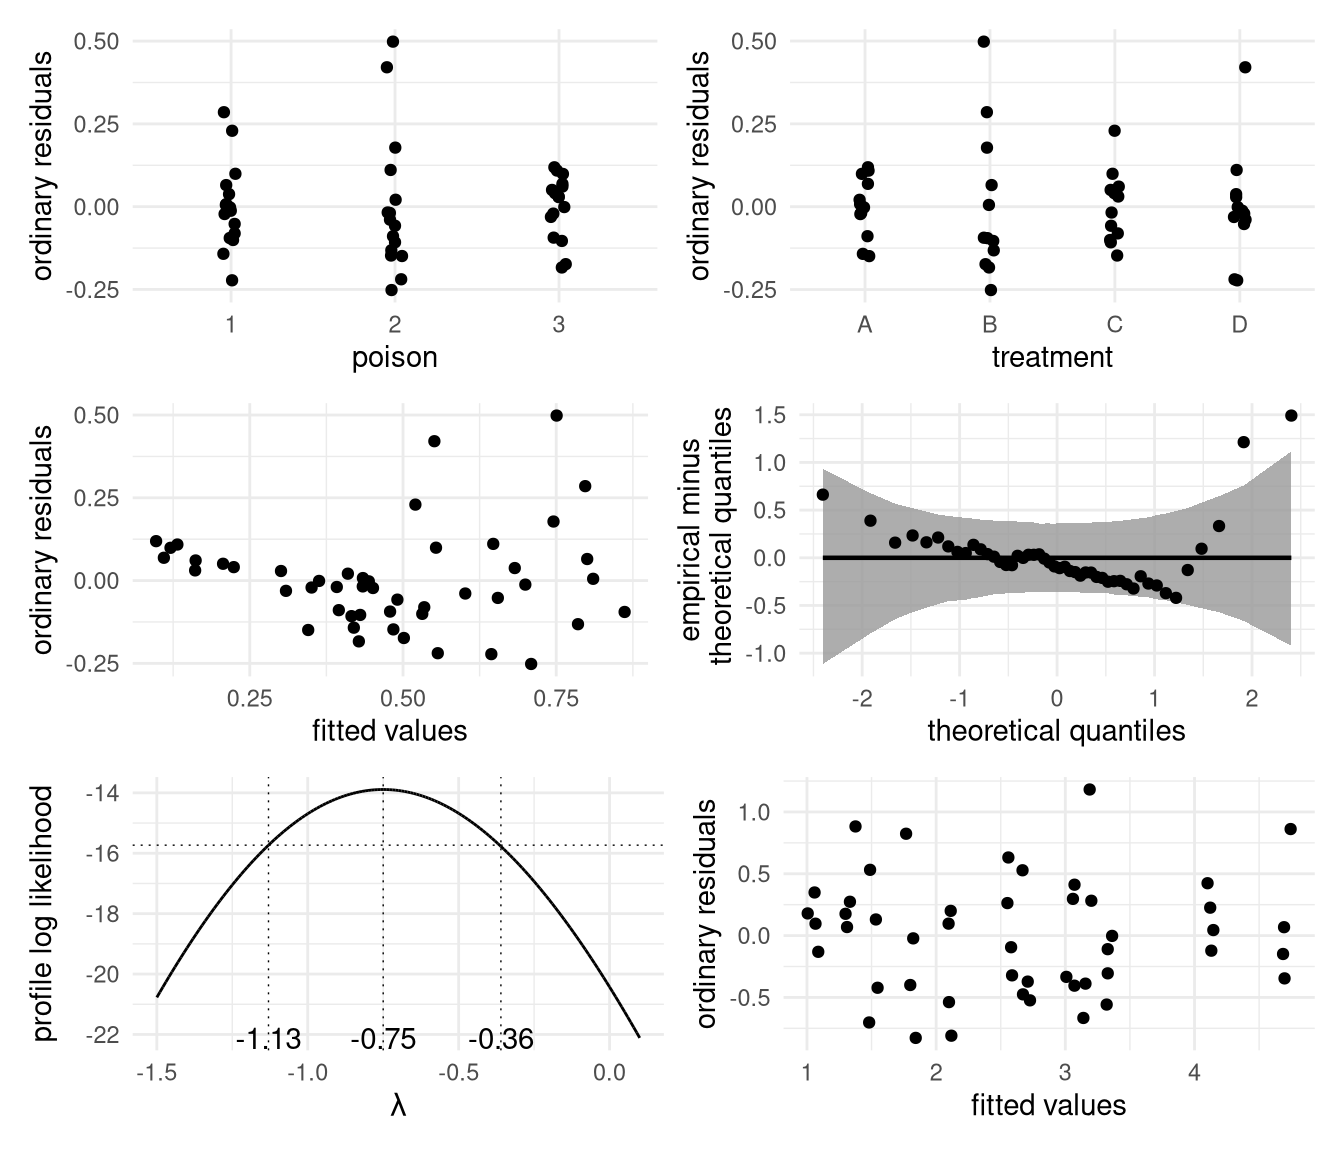
\includegraphics[width=0.7\linewidth]{MATH60604A_Statistical_modelling_files/figure-latex/poisonplots-1} 

}

\caption{Diagnostic plots for the poison data. The top panel shows the ordinary residuals for the linear model for survival time as a function of poison and treatment, with jittered observations. The middle left plot shows the fitted values against residuals, which display evidence of trend and increase in variance with the survival time. The quantile-quantile plot in the middle right plot shows some evidence of departure from the normality, but the non-linearity and heteroscedasticity obscure this. The bottom panel shows the profile log likelihood for the Box--Cox transform, suggesting a value of $-1$ would be within the 95\% confidence interval. After fitting the same additive model with main effect only to the reciprocal survival time, there is no more evidence of residual structure and unequal variance.}\label{fig:poisonplots}
\end{figure}

\hypertarget{likelihood}{%
\chapter{Likelihood-based inference}\label{likelihood}}

The goal of this chapter is to familiarize you with likelihood-based inference.

The starting point of likelihood-based inference is a statistical model: we postulate that (a function of) the data has been generated from a probability distribution with \(p\)-dimensional parameter vector \(\boldsymbol{\theta}\). The purpose of the analyst is to estimate these unknown parameters on the basis of a sample and make inference about them.

\hypertarget{maximum-likelihood}{%
\section{Maximum likelihood}\label{maximum-likelihood}}

The \textbf{likelihood} \(L(\boldsymbol{\theta})\) is a function of \(\boldsymbol{\theta}\) that gives the probability (or density) of observing a sample under a postulated distribution, treating the observations as fixed. In most settings we consider, observations are independent and so the joint probability of the sample values is the product of the probability of the individual observations\footnote{If this seems foreign, think about repeated coin tosses with Bernoulli distribution of unknown parameter \(p\) and convince yourself that the trials are independent, so the probability of obtaining two consecutive heads is \(0.25\) for a fair coin.}: for \(y_1, \ldots, y_n\) assuming \(Y_i\) (\(i=1, \ldots, n\)) follows a distribution whose mass function or density is \(f(y; \boldsymbol{\theta})\), this is just
\begin{align*}
L(\boldsymbol{\theta}; \boldsymbol{y}) = \prod_{i=1}^n f(y_i; \boldsymbol{\theta}) = f(y_1; \boldsymbol{\theta}) \times \cdots \times f(y_n; \boldsymbol{\theta}).
\end{align*}

From a pure optimization perspective, the likelihood is a particular choice of objective function that reflects the probability of the observed outcome. One shouldn't however maximize directly the likelihood, since computing the product of a lot of potentially small numbers is subject to numerical overflow and is unstable (for discrete distributions, the mass function gives probabilities that are by definition between zero and one). Instead, one should work with the log likelihood function, \(\ell(\boldsymbol{\theta}) = \ln\{L(\boldsymbol{\theta})\}\). Since logarithm is a strictly increasing function, maximizing the natural logarithm (denoted \(\ln\)) of the likelihood leads to the same solution. Another reason why working with the log likelihood is preferable is because product over \(n\) likelihood contributions becomes a sum and this facilitates numerical and analytical derivations of the maximum likelihood estimators (the log of a product is equal to the sum of logs, i.e., \(\ln(ab) =\ln(a) +\ln(b)\) for \(a, b>0\).)

The \textbf{maximum likelihood estimator} \(\widehat{\boldsymbol{\theta}}\) is the value of \(\boldsymbol{\theta}\) that maximizes the likelihood, i.e., the value under which the random sample is the most likely to be generated. The scientific reasoning behind this is: ``whatever we observe, we have expected to observe'' so we choose between competing models the one that makes the most sense.

Several properties of maximum likelihood estimator makes it appealing for inference.

\begin{itemize}
\tightlist
\item
  The maximum likelihood estimator is \textbf{consistent}, i.e., it converges to the correct value as the sample size increase (asymptotically unbiased).
\item
  The maximum likelihood estimator is invariant to reparametrizations
\item
  Under regularity conditions, the maximum likelihood estimator is asymptotically normal, so we can obtain the null distribution of classes of hypothesis tests and derive confidence intervals based on \(\widehat{\boldsymbol{\theta}}\).
\item
  The maximum likelihood estimator is efficient, meaning it has the smallest asymptotic mean squared error (or the smallest asymptotic variance).
\end{itemize}

The \textbf{score function} \(U(\boldsymbol{\theta}; \boldsymbol{y}) = \partial \ell(\boldsymbol{\theta}; \boldsymbol{y})/ \partial \boldsymbol{\theta}\) is the gradient of the log likelihood function and, under regularity conditions, the maximum likelihood estimator solves \(U(\boldsymbol{\theta}; \boldsymbol{Y})=\boldsymbol{0}_p\). This property can be used to derive gradient-based algorithms for optimization and for verifying that the solution found is a global maximum.

\begin{remark}
\iffalse{} {Remark. } \fi{}While least squares admit a closed-form solution, the maximum of the log likelihood is generally found numerically by solving the score equation. The algorithms used in most software are reliable and efficient for regression models we consider in this course. However, for more complex models, like generalized linear mixed models, the convergence of optimization algorithms is oftentimes problematic and scrutiny is warranted.
\end{remark}

The \textbf{observed information matrix} is the hessian \(j(\boldsymbol{\theta}; \boldsymbol{y})=-\partial^2 \ell(\boldsymbol{\theta}; \boldsymbol{y})/\partial \boldsymbol{\theta} \partial \boldsymbol{\theta}^\top\) evaluated at the maximum likelihood estimate \(\widehat{\boldsymbol{\theta}}\).
Under regularity conditions, the Fisher information matrix is
\begin{align*}
i(\boldsymbol{\theta}) = \mathsf{E}\left\{U(\boldsymbol{\theta}; \boldsymbol{Y}) U(\boldsymbol{\theta}; \boldsymbol{Y})^\top\right\} = \mathsf{E}\left\{j(\boldsymbol{\theta}; \boldsymbol{Y})\right\}
\end{align*}
The Fisher (or expected) and observed information matrices encodes the curvature of the log likelihood and provides information about the variability of \(\widehat{\boldsymbol{\theta}}\).

The properties of the log likelihood are particularly convenient for inference because they provide omnibus testing procedures that have a known asymptotic distribution. The starting point for the distributional theory surrounding likelihood-based statistics is the asymptotic normality of the score \(U(\boldsymbol{\theta}) \stackrel{\cdot}{\sim}\mathsf{No}(0, i(\boldsymbol{\theta}))\), which follows from a central limit theorem. The variance of \(U(\boldsymbol{\theta}_0)\) is exactly \(i(\boldsymbol{\theta}_0)\), while that of \(\widehat{\boldsymbol{\theta}}\) is approximately \(i(\boldsymbol{\theta}_0)^{-1}\) under the null hypothesis \(\mathscr{H}_0\). This result is particularly useful: we often use the inverse of the observed information as estimate of the covariance matrix of the maximum likelihood estimator. To obtain the standard errors of \(\widehat{\boldsymbol{\theta}}\), one simple computes the square root of the diagonal elements of the inverse of the observed information, i.e., \([\mathrm{diag}\{j^{-1}(\widehat{\boldsymbol{\theta}})\}]^{1/2}\).

\begin{example}[Exponential model for waiting times of the Montreal metro]
\protect\hypertarget{exm:waitingtime}{}{\label{exm:waitingtime} \iffalse (Exponential model for waiting times of the Montreal metro) \fi{} }Consider the waiting time \(Y\) between consecutive subways arriving at Station Édouard-Montpetit on the blue line in Montreal during rush hour. We postulate that these waiting times follow an exponential distribution with rate \(\theta\), denoted \(Y \sim \mathsf{E}(\theta)\). The purpose of statistical inference is to use the information from a random sample of size \(n\) to estimate the unknown parameter \(\theta\). The density of \(Y\) evaluated at \(y\), \(f(y; \theta)=\theta\exp(-\theta y)\), encodes the probability of the observed waiting time for a given parameter value and, if the records are independent, the probability of observing \(y_1, \ldots, y_n\) is the product of probabilities of individual events. The likelihood is thus
\begin{align*}
L(\theta; \boldsymbol{y}) &= \prod_{i=1}^n f(y; \theta)= \prod_{i=1}^n\theta\exp(-\theta y_i),\\
\ell(\theta; \boldsymbol{y}) & = n\ln(\theta) - \theta\sum_{i=1}^n y_i
\end{align*}
To find the maximum of the function, we differentiate the log likelihood \(\ell(\theta; \boldsymbol{y})\) and set the gradient to zero,
\begin{align*}
\frac{\partial \ell(\theta; \boldsymbol{y})}{\partial \theta} & = \frac{n}{\theta} - \sum_{i=1}^n y_i =0.
\end{align*}
Solving for \(\theta\) gives \(\widehat{\theta} = \overline{y}^{-1}\), so the maximum likelihood estimator is the reciprocal of the sample mean \(\overline{Y}\). The observed information is \(j(\theta) = n\theta^{-2}\) and likewise \(i(\theta)=\mathsf{E}\{j(\theta)\}=n\theta^{-2}\).
\end{example}

\begin{figure}

{\centering 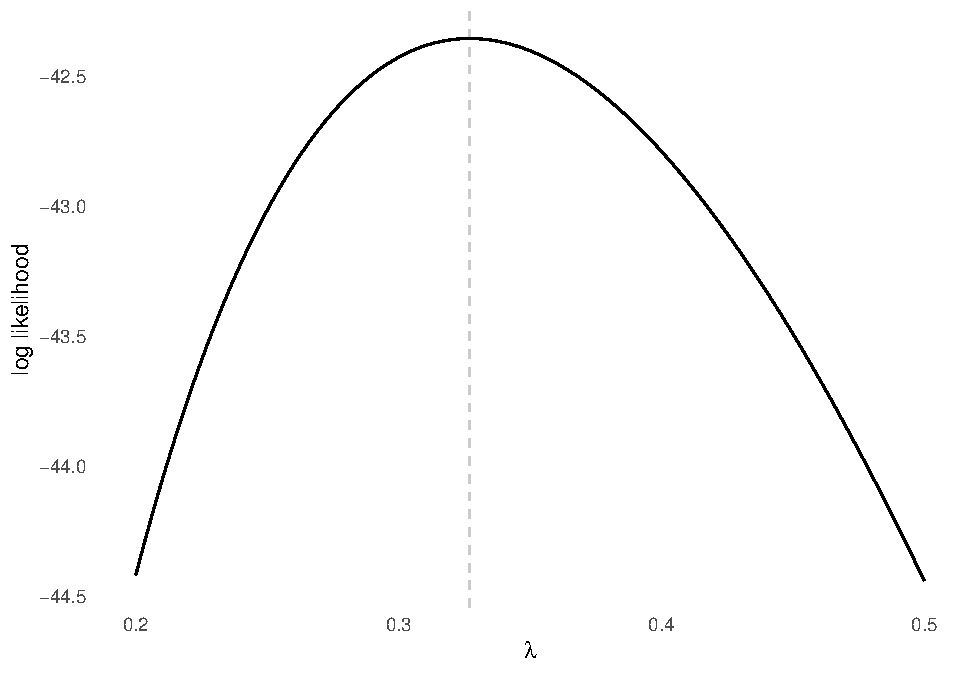
\includegraphics[width=0.7\linewidth]{MATH60604A_Statistical_modelling_files/figure-latex/explikelihood-1} 

}

\caption{Log-likelihood for a sample of size 20 of waiting times (in minutes)}\label{fig:explikelihood}
\end{figure}

For the sample of waiting time in the subway, the maximum likelihood estimate of \(\theta\) is \(\widehat{\theta}=0.327\), the observed information is \(j(\widehat{\theta})=i(\widehat{\theta})=0.467\) and the standard error of \(\widehat{\theta}\) is \(j(\widehat{\theta})^{-1/2}=1.463\).

\begin{example}[Normal samples and ordinary least squares]
\protect\hypertarget{exm:normal}{}{\label{exm:normal} \iffalse (Normal samples and ordinary least squares) \fi{} }Suppose we have an independent normal sample of size \(n\) with mean \(\mu\) and variance \(\sigma^2\), where
\(Y_i \sim \mathsf{No}(\mu, \sigma^2)\) are independent.
Recall that the density of the normal distribution is
\begin{align*}
f(\boldsymbol{y}; \mu, \sigma^2)=\frac{1}{(2\pi \sigma^2)^{1/2}}\exp\left\{-\frac{1}{2\sigma^2}(x-\mu)^2\right\}.
\end{align*}
For an \(n\)-sample \(\boldsymbol{y}\), the likelihood is
\begin{align*}
L(\mu, \sigma^2; \boldsymbol{y})=&\prod_{i=1}^n\frac{1}{({2\pi \sigma^2})^{1/2}}\exp\left\{-\frac{1}{2\sigma^2}(y_i-\mu)^2\right\}\\
=&(2\pi \sigma^2)^{-n/2}\exp\left\{-\frac{1}{2\sigma^2}\sum_{i=1}^n(y_i-\mu)^2\right\}.
\end{align*}
and the log likelihood is
\begin{align*}
\ell(\mu, \sigma^2; \boldsymbol{y})=-\frac{n}{2}\ln(2\pi) -\frac{n}{2}\ln(\sigma^2)-\frac{1}{2\sigma^2}\sum_{i=1}^n (y_i-\mu)^2.
\end{align*}

One can show that the maximum likelihood estimators for the two parameters are
\begin{align*}
\widehat{\mu}=\overline{Y}=\frac{1}{n} \sum_{i=1}^n Y_i, \qquad \widehat{\sigma}^2=\frac{1}{n}\sum_{i=1}^n (Y_i-\overline{Y})^2.
\end{align*}

The fact that the estimator of the theoretical mean \(\mu\) is the sample mean is fairly intuitive and one can show the estimator is unbiased for \(\mu\). The (unbiased) sample variance estimator,
\begin{align*}
S^2=\frac{1}{n-1} \sum_{i=1}^n (\mathrm{Y}_i-\overline{Y})^2
\end{align*}
Since \(\widehat{\sigma}^2=(n-1)/n S^2\), it follows that the maximum likelihood estimator of \(\sigma^2\) is biased, but both estimators are consistent and will thus get arbitrarily close to the true value \(\sigma^2\) for \(n\) sufficiently large.

The case of normally distributed data is intimately related to linear regression and ordinary least squares: assuming normality of the errors, the least square estimators of \(\boldsymbol{\beta}\) coincide with the maximum likelihood estimator of \(\boldsymbol{\beta}\).

Recall the linear regression model,
\begin{align*}
Y_i=\beta_0+\beta_1 \mathrm{X}_{i1}+\beta_2 \mathrm{X}_{i2}+\ldots +\beta_p \mathrm{X}_{ip} + \varepsilon_i, \qquad  (i=1, \ldots, n),
\end{align*}
where the errors \(\varepsilon_i \sim \mathsf{No}(0, \sigma^2)\).
The linear model has \(p+2\) parameters (\(\boldsymbol{\beta}\) and \(\sigma^2\)) and the log likelihood is
\begin{align*}
\ell(\boldsymbol{\theta})&=-\frac{n}{2} \ln(2\pi)-\frac{n}{2} \ln (\sigma^2) -\frac{1}{2\sigma^2}\left\{\boldsymbol{y}-\mathbf{X}\boldsymbol{\beta})^\top(\boldsymbol{y}-\mathbf{X}\boldsymbol{\beta})\right\}^2.
\end{align*}
Maximizing the log likelihood with respect to \(\boldsymbol{\beta}\) is equivalent to
minimizing the sum of squared errors \(\|\boldsymbol{Y} - \widehat{\boldsymbol{Y}}\|^2\). Since this objective function is the same as that of least squares, it follows that the least-square estimator \(\widehat{\boldsymbol{\beta}}\) for the mean parameters is the maximum likelihood estimator for normal errors with common variance \(\sigma^2\), regardless of the value of the latter. The maximum likelihood estimator \(\widehat{\sigma}^2\) is thus
\begin{align*}
\hat{\sigma}^2=\max_{\sigma^2} \ell(\widehat{\boldsymbol{\beta}}, \sigma^2).
\end{align*}
The log likelihood, excluding constant terms that don't depend on \(\sigma^2\), is
\begin{align*}
\ell(\widehat{\boldsymbol{\beta}}, \sigma^2)
&\propto-\frac{1}{2}\left\{n\ln\sigma^2+\frac{1}{\sigma^2}(\boldsymbol{y}-\mathbf{X}\hat{\boldsymbol{\beta}})^\top(\boldsymbol{y}-\mathbf{X}\hat{\boldsymbol{\beta}})\right\}.
\end{align*}
Differentiating each term with respect to \(\sigma^2\) and setting the gradient equal to zero yields the maximum likelihood estimator
\begin{align*}
\hat{\sigma}^2=\frac{1}{n}(\boldsymbol{Y}-\mathbf{X}\hat{\boldsymbol{\beta}})^\top(\boldsymbol{Y}-\mathbf{X}\hat{\boldsymbol{\beta}})= \frac{1}{n} \sum_{i=1}^n e_i^2= \frac{\mathsf{SS}_e}{n};
\end{align*}
where \(\mathsf{SS}_e\) is the sum of squared residuals. The usual unbiased estimator of \(\sigma^2\) calculated by software is \(S^2=\mathsf{SS}_e/(n-p-1)\), where the denominator is the sample size \(n\) minus the number of mean parameters \(\boldsymbol{\beta}\), \(p+1\).
\end{example}

Sometimes, the \(p\)-parameter vector \(\boldsymbol{\theta}\) of the likelihood is not the quantity of interest. Suppose for simplicity we are interested in a scalar function \(\phi = g(\boldsymbol{\theta})\). The maximum likelihood estimate of \(\phi\) is \(\widehat{\phi}=g(\widehat{\boldsymbol{\theta}})\). This property of maximum likelihood estimators justifies their widespread use. In large samples, \(\widehat{\boldsymbol{\theta}}\) is centered at the true value \(\boldsymbol{\theta}_0\) and is approximately multivariate normal with \(\widehat{\boldsymbol{\theta}} \stackrel{\cdot}{\sim} \mathsf{No}_p(\boldsymbol{\theta}_0, \mathbf{V}_{\boldsymbol{\theta}})\), then
\(\widehat{\phi} \stackrel{\cdot}{\sim}\mathsf{No}(\phi_0, \mathrm{V}_\phi)\), with \(\mathrm{V}_\phi = \nabla \phi^\top \mathbf{V}_{\boldsymbol{\theta}} \nabla \phi\), where \(\nabla \phi=[\partial \phi/\partial \theta_1, \ldots, \partial \phi/\partial \theta_p]^\top\). In applications, the variance matrix and the gradient vector are evaluated at the maximum likelihood estimate \(\widehat{\boldsymbol{\theta}}\)

Consider the metro waiting time example. The quantity of interest is the reciprocal mean \(\phi = 1/\theta\), so the scalar function of interest is \(g(x) = 1/x\) and the maximum likelihood estimate \(\hat{\phi}=3.058\) is the sample mean of waiting times. The gradient of the transformation is \(\nabla \phi = -1/x^2\), which gives \(\mathrm{V}_\phi = (\theta^2/n)/\theta^4 = 1/(n\theta^2) = \phi^2/n\) and the standard error of the maximum likelihood estimator is thus approximately \(\widehat{\phi}/\sqrt{n}\) in large samples.

\hypertarget{liktests}{%
\section{Likelihood-based tests}\label{liktests}}

Oftentimes, we wish to compare two models: the model implied by the null hypothesis, which is a restriction or simpler version of the full model. Models are said to be \textbf{nested} if we can obtain one from the other by imposing restrictions on the parameters.

We consider a null hypothesis \(\mathscr{H}_0\) that imposes restrictions on the possible values of \(\boldsymbol{\theta}\) can take, relative to an unconstrained alternative \(\mathscr{H}_1\). We need two \textbf{nested} models: a \emph{full} model, and a \emph{reduced} model that is a subset of the full model where we impose \(q\) restrictions. For example, the full model could be a regression model with four predictor variables and the reduced model could include only the first two predictor variables, which is equivalent to setting \(\mathscr{H}_0: \beta_3=\beta_4=0\). The testing procedure involves fitting the two models and obtaining the maximum likelihood estimators of each of \(\mathscr{H}_1\) and \(\mathscr{H}_0\), respectively \(\widehat{\boldsymbol{\theta}}\) and \(\widehat{\boldsymbol{\theta}}_0\) for the parameters under \(\mathscr{H}_0\).
The null hypothesis \(\mathscr{H}_0\) tested is: `the reduced model is an \textbf{adequate simplification} of the full model' and the likelihood provides three main classes of statistics for testing this hypothesis: these are

\begin{itemize}
\tightlist
\item
  likelihood ratio tests statistics, denoted \(R\), which measure the drop in log likelihood (vertical distance) from \(\ell(\widehat{\boldsymbol{\theta}})\) and \(\ell(\widehat{\boldsymbol{\theta}}_0)\).
\item
  Wald tests statistics, denoted \(W\), which consider the standardized horizontal distance between \(\widehat{\boldsymbol{\theta}}\) and \(\widehat{\boldsymbol{\theta}}_0\).
\item
  score tests statistics, denoted \(S\), which looks at the scaled gradient of \(\ell\), evaluated \emph{only} at \(\widehat{\boldsymbol{\theta}}_0\) (derivative of \(\ell\)).
\end{itemize}

\begin{figure}

{\centering 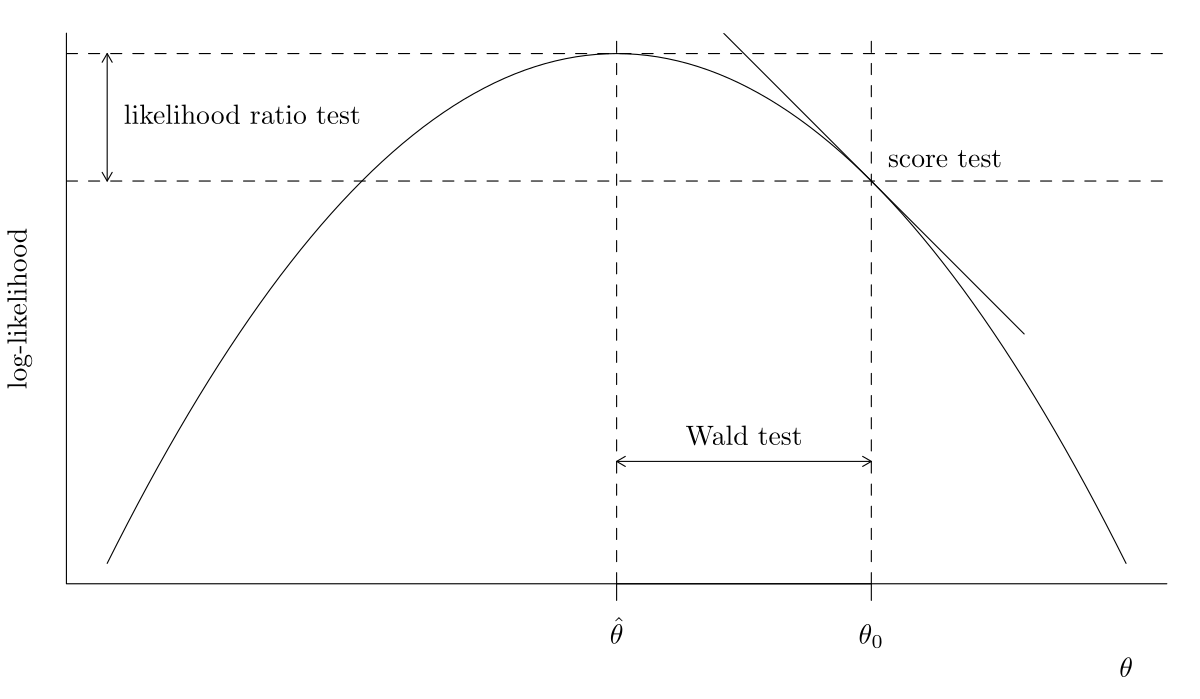
\includegraphics[width=0.7\linewidth]{images/likelihood_tests} 

}

\caption{Log-likelihood curve: the three likelihood-based tests, namely Wald, likelihood ratio and score tests, are shown on the curve. The tests use different information about the function.}\label{fig:variablesquanti}
\end{figure}

The three main classes of statistics for testing a simple null hypothesis \(\mathscr{H}_0: \boldsymbol{\theta}=\boldsymbol{\theta}_0\) against the alternative \(\mathscr{H}_a: \boldsymbol{\theta} \neq \boldsymbol{\theta}_0\) are the likelihood ratio, the score and the Wald statistics, defined respectively as
\begin{align*}
 R &= 2 \left\{ \ell(\widehat{\boldsymbol{\theta}})-\ell(\boldsymbol{\theta}_0)\right\}, \\
 S &= U^\top(\boldsymbol{\theta}_0)i^{-1}(\boldsymbol{\theta}_0)U(\boldsymbol{\theta}_0), \\
 W &= (\widehat{\boldsymbol{\theta}}-\boldsymbol{\theta}_0)^\top j(\widehat{\boldsymbol{\theta}})(\widehat{\boldsymbol{\theta}}-\boldsymbol{\theta}_0),
\end{align*}
where \(\widehat{\boldsymbol{\theta}}\) is the maximum likelihood estimate under the alternative and \(\boldsymbol{\theta}_0\) is the null value of the parameter vector. Asymptotically, all the test statistics are equivalent (in the sense that they lead to the same conclusions about \(\mathscr{H}_0\)).
If \(\mathscr{H}_0\) is true, the three test statistics follow asymptotically a \(\chi^2_q\) distribution under a null hypothesis \(\mathscr{H}_0\), where the degrees of freedom \(q\) are the number of restrictions.

For scalar \(\theta\) with \(q=1\), signed versions of these statistics exist, e.g., \begin{align*}
W(\theta_0)=(\widehat{\theta}-\theta_0)/\mathsf{se}(\widehat{\theta})\stackrel{\cdot}{\sim} \mathsf{No}(0,1)
\end{align*}
for the Wald statistic or the directed likelihood root
\begin{align*}
R({\theta_0}) = \mathrm{sign}(\widehat{\theta}-\theta)\left[2
\left\{\ell(\widehat{\theta})-\ell(\theta)\right\}\right]^{1/2} \stackrel{\cdot}{\sim} \mathsf{No}(0,1).
\end{align*}
The likelihood ratio test statistic is normally the most powerful of the three likelihood tests. The score statistic \(S\) only requires calculation of the score and information under \(\mathscr{H}_0\) (because by definition \(U(\widehat{\theta})=0\)), so it can be useful in problems where calculations of the maximum likelihood estimator under the alternative is costly or impossible.

The Wald statistic \(W\) is the most widely encountered statistic and two-sided 95\% confidence intervals for a single parameter \(\theta\) are of the form
\begin{align*}
\widehat{\theta} \pm q_{1-\alpha/2}\mathrm{se}(\widehat{\theta}),
\end{align*}
where \(q_{1-\alpha/2}\) is the \(1-\alpha/2\) quantile of the standard normal distribution; for a \(95\)\% confidence interval, the \(0.975\) quantile of the normal distribution is \(1.96\).
The Wald-based confidence intervals are by construction \textbf{symmetric}: they may include implausible values (e.g., negative values for variances). The Wald-based confidence intervals are not parametrization invariant: if we want intervals for a nonlinear continuous function \(g(\theta)\), then in general
\(\mathsf{CI}_{W}\{g(\theta)\} \neq g\{\mathsf{CI}_{W}(\theta)\}.\)

These confidence intervals can be contrasted with the (better) ones derived using the likelihood ratio test: these are found through a numerical search to find the limits of
\begin{align*}
\theta: 2\{\ell(\widehat{\theta}) - \ell(\theta)\} \leq \chi^2_1(1-\alpha),
\end{align*}
where \(\chi^2_1(1-\alpha)\) is the \((1-\alpha)\) quantile of the \(\chi^2_1\) distribution. If \(\boldsymbol{\theta}\) is multidimensional, confidence intervals for \(\theta_i\) are derived using the profile likelihood. Likelihood ratio-based confidence intervals are \textbf{parametrization invariant}, so \(\mathsf{CI}_{R}\{g(\theta)\} = g\{\mathsf{CI}_{R}(\theta)\}\). Because the likelihood is zero if a parameter value falls outside the range of possible values for the parameter, the intervals only include plausible values of \(\theta\). In general, the intervals are asymmetric and have better coverage properties.

To illustrate the difference between likelihood ratio and Wald tests (and their respective confidence intervals), we consider the metro waiting time data and consider a two-sided test for the null hypothesis \(\mathscr{H}_0: \phi_0=4\) minutes. The Wald statistic is
\begin{align*}
W =\frac{\hat{\phi}-\phi_0}{\mathsf{se}(\widehat{\phi})}=\sqrt{n}\frac{\widehat{\phi}-\phi_0}{\widehat{\phi}}= -1.378,
\end{align*}
since \(\mathsf{se}(\phi)=\mathrm{V}^{1/2}_{\phi}=\phi/\sqrt{n}\) and the latter function is evaluated at \(\widehat{\phi}=3.058\). The asymptotic null distribution is \(\mathsf{No}(0,1)\), so we fail to reject \(\mathscr{H}_0: \phi=4\) minutes since the observed value for \(|W|\) is smaller than \(1.96\). We could invert the test statistic to get a symmetric 95\% confidence interval for \(\phi\), \([1.718\), \(4.398]\).

The hypothesis corresponds also to \(\theta=0.25\) and similar calculations give \(W = \sqrt{n}(0.327 - 0.25)/0.327 = 1.053\). In this case, the null distribution is the same, but the value of the test statistic is not! The confidence interval for \(\theta\) is \([0.184\), \(0.47]\). You can check for yourself that the reciprocal of these confidence intervals do not match those for \(\phi\).

In contrast, the likelihood ratio test is invariant to interest-preserving reparamtrizations, so the test statistic for \(\mathscr{H}_0: \phi=4\) and \(\mathscr{H}_0: \theta = 0.25\) are the same. The log likelihood at \(\theta=0.25\) is -43.015, the maximum log likelihood value is -42.354
and the likelihood ratio statistic \(R=2 \{\ell(\widehat{\theta}) - \ell(4)\}= 1.322\). The statistic should behave like a \(\chi^2_1\) variable in large samples. The 95\% of the \(\chi^2_1\) distribution is \(3.841\), so we fail to reject the null hypothesis that the mean waiting time is 4 minutes.

The likelihood ratio statistic 95\% confidence interval for \(\phi\) can be found by using a root finding algorithm: the confidence interval is \([2.032\), \(4.906]\). By invariance, the 95\% confidence interval for \(\theta\) is \([0.204, 0.492]\).

\hypertarget{profile-likelihood}{%
\section{Profile likelihood}\label{profile-likelihood}}

Sometimes, we may want to perform hypothesis test or derive confidence intervals for selected components of the model. For example, we may be interested in obtaining confidence intervals for a single \(\beta_j\) in a logistic regression, treating the other parameters \(\boldsymbol{\beta}_{-j}\) as nuisance In this case, the null hypothesis only restricts part of the space and the other parameters, termed nuisance, are left unspecified --- the question then is what values to use for comparison with the full model. It turns out that the values that maximize the constrained log likelihood are what one should use for the test, and the particular function in which these nuisance parameters are integrated out is termed a profile likelihood.

Consider a parametric model with log likelihood function \(\ell(\boldsymbol{\theta})\) whose \(p\)-dimensional parameter vector \(\boldsymbol{\theta}=(\boldsymbol{\psi}, \boldsymbol{\lambda})\) that can be decomposed into a \(q\)-dimensional parameter of interest \(\boldsymbol{\psi}\) and a \((p-q)\)-dimensional nuisance vector \(\boldsymbol{\lambda}\).

We can consider the profile likelihood \(\ell_{\mathsf{p}}\), a function of \(\boldsymbol{\psi}\) alone, which is obtained by maximizing the likelihood pointwise at each fixed value \(\boldsymbol{\psi}_0\) over the nuisance vector \(\boldsymbol{\varphi}_{\psi_0}\),
\begin{align*}
\ell_{\mathsf{p}}(\boldsymbol{\psi})=\max_{\boldsymbol{\varphi}}\ell(\boldsymbol{\psi}, \boldsymbol{\varphi})=\ell(\boldsymbol{\psi}, \widehat{\boldsymbol{\varphi}}_{\boldsymbol{\psi}}).
\end{align*}
Figure \ref{fig:profile3d} shows a fictional log likelihood contour plot with the resulting profile curve (in black), where the log likelihood value is mapped to colors. If one thinks of these contours lines as those of a topographic map, the profile likelihood corresponds in this case to walking along the ridge of both mountains along the \(\psi\) direction, with the right panel showing the elevation gain/loss.

The maximum profile likelihood estimator behaves like a regular likelihood for most quantities of interest and we can derive test statistics and confidence intervals in the usual way. One famous example of profile likelihood is the Cox proportional hazard covered in \protect\hyperlink{survival}{Chapter 7}.

\begin{figure}

{\centering 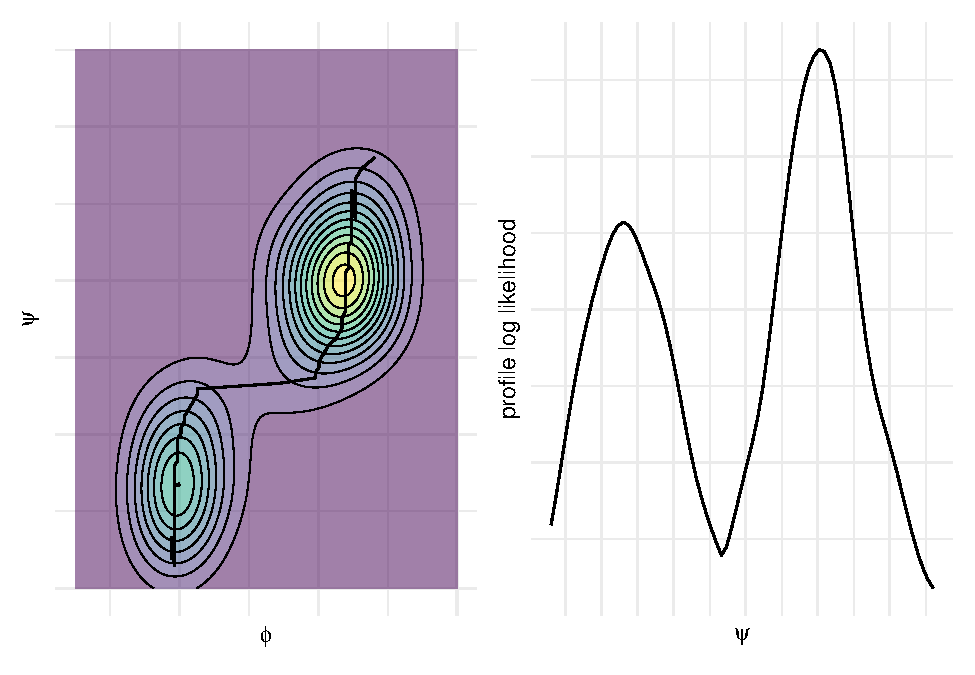
\includegraphics[width=0.7\linewidth]{MATH60604A_Statistical_modelling_files/figure-latex/profile3d-1} 

}

\caption{Two-dimensional log likelihood surface with a parameter of interest $\psi$ and a nuisance parameter $\varphi$; the contour plot shows area of higher likelihood, and the black line is the profile log likelihood, also shown as a function of $\psi$ on the right panel.}\label{fig:profile3d}
\end{figure}

\begin{example}[Box--Cox transformation]
\protect\hypertarget{exm:boxcox}{}{\label{exm:boxcox} \iffalse (Box--Cox transformation) \fi{} }Sometimes, the assumption of normality of the error doesn't hold. If the data are strictly positive, one can consider a Box--Cox transformation,
\begin{align*}
y_i(\lambda)= \begin{cases}
(y^{\lambda}-1)/\lambda, & \lambda \neq 0\\
\ln(y), & \lambda=0.
\end{cases}
\end{align*}

If we assume that \(\boldsymbol{y}(\lambda) \sim \mathsf{No}(\mathbf{X}\boldsymbol{\beta}, \sigma^2 \mathbf{I}_n)\), then the likelihood of \(\boldsymbol{y}\) is
\begin{align*}
L(\lambda, \boldsymbol{\beta}, \sigma; \boldsymbol{y}, \mathbf{X}) = (2\pi\sigma^2)^{-n/2}\exp \left[ - \frac{1}{2\sigma^2}\{\boldsymbol{y}(\lambda) - \mathbf{X}\boldsymbol{\beta}\}^\top\{\boldsymbol{y}(\lambda) - \mathbf{X}\boldsymbol{\beta}\}\right] J(\lambda, \boldsymbol{y}),
\end{align*}
where \(J\) denotes the Jacobian of the Box--Cox transformation, \(\prod_{i=1}^n y_i^{\lambda-1}\).
For each given value of \(\lambda\), the maximum likelihood estimator is that of the usual regression model, with \(\boldsymbol{y}\) replaced by \(\boldsymbol{y}(\lambda)\), namely \(\widehat{\boldsymbol{\beta}}_\lambda = (\mathbf{X}^\top\mathbf{X})^{-1}\mathbf{X}^\top \boldsymbol{y}(\lambda)\) and \(\widehat{\sigma}^2_\lambda = n^{-1}\{ \boldsymbol{y}(\lambda) - \mathbf{X}\widehat{\boldsymbol{\beta}}_\lambda\}^\top\{ \boldsymbol{y}(\lambda) - \mathbf{X}\widehat{\boldsymbol{\beta}}_\lambda\}\).

The profile log likelihood is
\begin{align*}
\ell_{\mathsf{p}}(\lambda) = -\frac{n}{2}\ln(2\pi \widehat{\sigma}^2_\lambda) - \frac{n}{2} + (\lambda - 1)\sum_{i=1}^n \ln(y_i)
\end{align*}
The maximum profile likelihood estimator is the value \(\lambda\) minimizes the sum of squared residuals from the linear model with \(\boldsymbol{y}(\lambda)\) as response.
\end{example}

\begin{figure}

{\centering 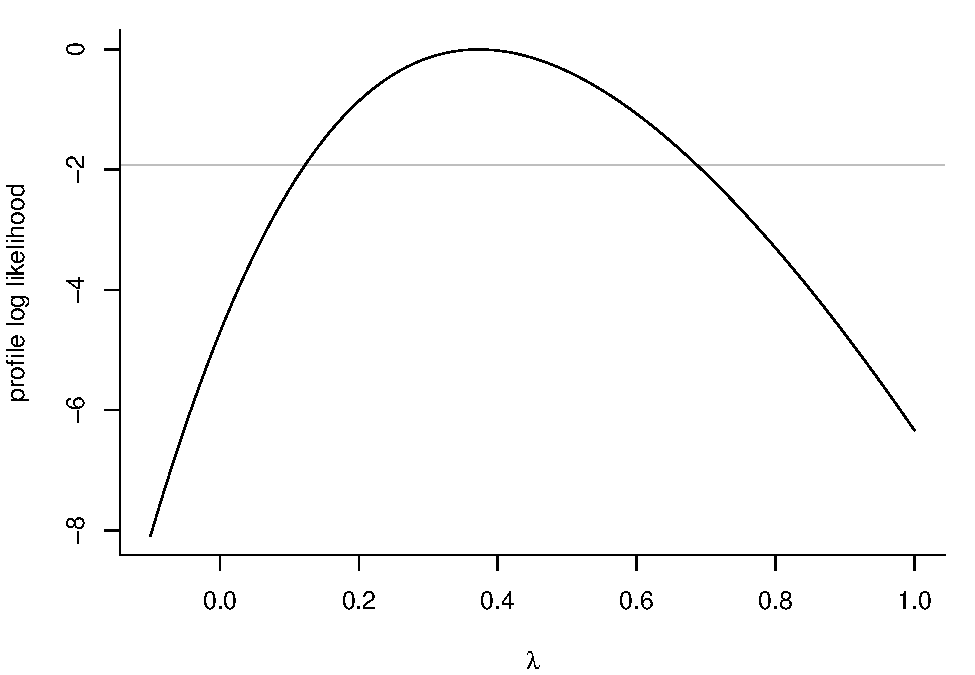
\includegraphics[width=0.7\linewidth]{MATH60604A_Statistical_modelling_files/figure-latex/profileplot-1} 

}

\caption{Profile log likelihood for the Box--Cox transformation for the waiting time data}\label{fig:profileplot}
\end{figure}

Figure \ref{fig:profileplot} shows the profile log likelihood for the linear model with an intercept-only, rescaled to be zero at the maximum. The function shows that a value of approximately \(0.37\) would provide residuals that are closer to normally distributed. The 95\% profile-likelihood based confidence interval is given by the two values of \(\lambda\), \((0.12, 0.69)\), at which the curve intersects the horizontal grey line drawn at \(-\chi^2_1/2\). The Box--Cox is not a panacea and should be reserved to cases where the transformation reduces heteroscedasticity (unequal variance) or creates a linear relation between explanatories and response: theory provides a cogent explanation of the data (e.g., the Cobb--Douglas production function used in economics can be linearized by taking a log-transformation). Rather than an \emph{ad hoc} choice of transformation, one could choose a log transformation if the value \(0\) is included within the 95\% confidence interval since this improves interpretability.

We could use the profile likelihood ratio test to obtain confidence intervals for the regression coefficients of the mean model. Consider for simplicity the normal simple linear model, \(\boldsymbol{Y} \sim \mathsf{No}_n(\beta_0 + \beta_1\mathbf{X}_1, \sigma^2)\). The profile for the slope parameter \(\beta_1\) can be obtained by maximizing the log likelihood for fixed \(\beta_1=b\), say: to achieve this, note that this amounts to \(\boldsymbol{Y}-b\mathbf{X}_1 \sim \mathsf{No}_n(\beta_0, \sigma^2)\) and so the estimator would correspond to
\begin{align*}
\widehat{\beta}_{0}^{(b)}&=\frac{1}{n} \sum_{i=1}^n (Y_i-b\mathrm{X}_i)\\
\widehat{\sigma}^{2(b)} &= \frac{1}{n}\sum_{i=1}^n \left(Y_i-b\mathrm{X}_i-\widehat{\beta}_{0}^{(b)}\right)^2.
\end{align*}
With more than one covariate, we could obtain the value of \(\boldsymbol{\beta}_{-j}^{(b)}\) by running least squares and use the residuals to compute the maximum likelihood estimate \(\widehat{\sigma}^{2(b)}\) of the variance.

\begin{figure}

{\centering 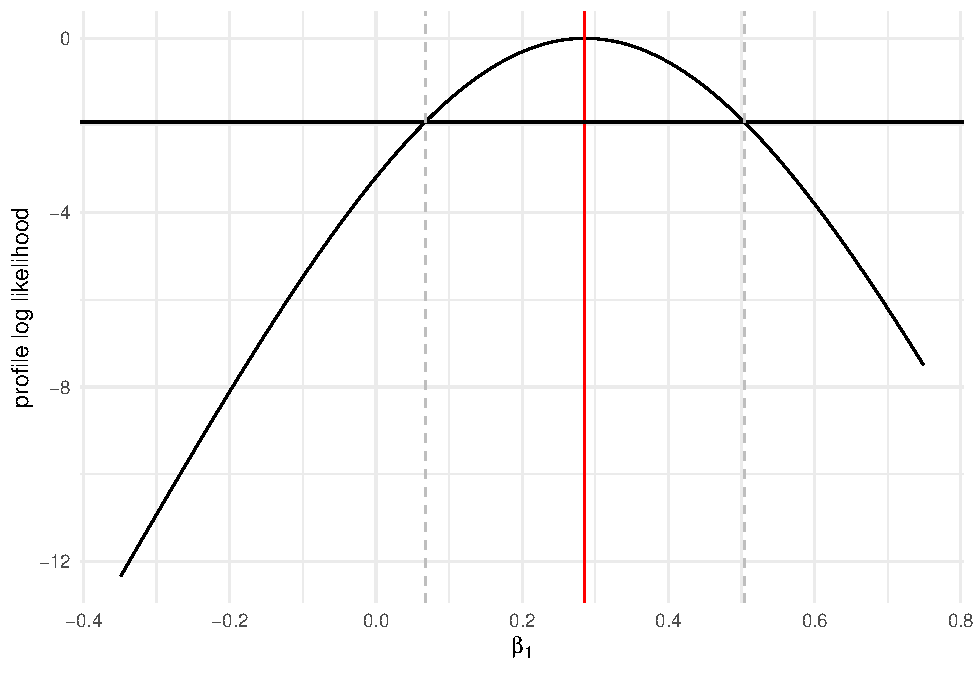
\includegraphics[width=0.7\linewidth]{MATH60604A_Statistical_modelling_files/figure-latex/profilebeta-1} 

}

\caption{Profile log likelihood for $\beta_1$ in the simple linear regression model for simulated data. The function has been so its value at the maximum likelihood estimate is zero. The horizontal cutoff marks minus half the $0.95$ quantile of the $\chi^2_1$ distribution, with vertical lines indicating the maximum likelihood estimate (red) and 95\% confidence interval (dashed gray). Because of the normality assumption of the linear regression model, the sampling distribution is exactly normally distribution, the profile is symmetric and the Wald and profile likelihood ratio based confidence intervals agree.}\label{fig:profilebeta}
\end{figure}

\hypertarget{information-criteria}{%
\section{Information criteria}\label{information-criteria}}

The likelihood can also serve as building block for model comparison: the larger \(\ell(\boldsymbol{\widehat{\theta}})\), the better the fit. However, the likelihood doesn't account for model complexity in the sense that more complex models with more parameters lead to higher likelihood. This is not a problem for comparison of nested models using the likelihood ratio test because we look only at relative improvement in fit. There is a danger of \textbf{overfitting} if we only consider the likelihood of a model.

\(\mathsf{AIC}\) and \(\mathsf{BIC}\) are information criteria measuring how well the model fits the data, while penalizing models with more parameters,
\begin{align*}
\mathsf{AIC}&=-2\ell(\widehat{\boldsymbol{\theta}})+2k \\
\mathsf{BIC}&=-2\ell(\widehat{\boldsymbol{\theta}})+k\ln(n),
\end{align*}
where \(k\) is the number of parameters in the model. The smaller the value of \(\mathsf{AIC}\) (or of \(\mathsf{BIC}\)), the better the model fit.

Note that information criteria do not constitute formal hypothesis tests on the parameters, but they can be used to compare non nested-models, even these estimates are particularly noisy. If we want to compare likelihood from different probability models, we need to make sure they include normalizing constant. The \(\mathsf{BIC}\) is more stringent than \(\mathsf{AIC}\), as its penalty increases with the sample size, so it selects models with fewer parameters. The \(\mathsf{BIC}\) is \textbf{consistent}, meaning that it will pick the true correct model from an ensemble of models with probability one as \(n \to \infty\). In practice, this is of little interest if one assumes that all models are approximation of reality (it is unlikely that the true model is included in the ones we consider). \(\mathsf{AIC}\) often selects overly complicated models in large samples, whereas \(\mathsf{BIC}\) is sometimes too conservative in that it chooses models that are overly simple.

\hypertarget{generalized-linear-models}{%
\chapter{Generalized linear models}\label{generalized-linear-models}}

Linear models are only suitable for data that are (approximately)
normally distributed. However, there are many settings where we may wish
to analyze a response variable which is not necessarily continuous,
including when \(Y\) is binary, a count variable or is continuous, but
non-negative. We will consider in particular likelihood-based inference
for binary/proportion and counts data.

Generalized linear models (GLM) combine a model for the conditional mean
with a distribution for the response variable and a link function tying
predictors and parameters.

This chapter gives an introduction to generalized linear models and
focuses in particular on logistic regression and Poisson regression, but
only for the case of independent observations. Extensions of generalized
linear models for correlated and longitudinal data, the so-called
\emph{generalized linear mixed models} (GLMM), are covered in MATH80621.

\hypertarget{basic-principles}{%
\section{Basic principles}\label{basic-principles}}

The starting point is the same as for linear regression: we have a
random sample of independent observations
\((\boldsymbol{Y}, \mathbf{X})\), where \(Y\) is the response variable and
\(\mathrm{X}_1, \ldots, \mathrm{X}_p\) are \(p\) explanatory variables or
covariates which are assumed fixed (non-random). The goal is to model
the mean of the response variable as a function of the explanatory
variables.

Let \(\mu_i=\mathsf{E}(Y_i \mid \mathbf{X}_i)\) denote the conditional
expectation of \(Y_i\) given covariates and let \(\eta_i\) denote the linear
combination of the covariates that will be used to model the response
variable,
\begin{align*}
\eta_i=\beta_0 + \beta_1 \mathrm{X}_{i1} + \cdots + \beta_p \mathrm{X}_{ip}.
\end{align*}
The building blocks of the generalized linear model are

\begin{itemize}
\tightlist
\item
  A random component, consisting of the probability distribution for the outcome \(Y\) that is a member of the exponential dispersion family (normal, binomial, Poisson, gamma, \ldots).
\item
  A deterministic component, the \textbf{linear predictor} \(\boldsymbol{\eta}=\mathbf{X} \boldsymbol{\beta}\), where \(\mathbf{X}\) is an \(n\times (p+1)\) matrix with columns \(\mathbf{1}_n, \mathbf{X}_1, \ldots, \mathbf{X}_p\) and \(\boldsymbol{\beta} \in \mathbb{R}^{p+1}\) are coefficients.
\item
  A monotone function \(g\), called \textbf{link function}, that maps the mean of \(Y_i\) to the predictor variables, \(g(\mu_i)=\eta_i\).
\end{itemize}

\hypertarget{theory-of-generalized-linear-models}{%
\section{Theory of generalized linear models}\label{theory-of-generalized-linear-models}}

This section borrows from Chapter 4 of

\begin{quote}
Agresti (2015). \emph{Foundations of Linear and Generalized Linear Models}, Wiley.
\end{quote}

\hypertarget{exponential-dispersion-family-of-distributions}{%
\subsection{Exponential dispersion family of distributions}\label{exponential-dispersion-family-of-distributions}}

In a generalized linear model, the random component arises from an
exponential dispersion family. Consider a probability density or mass
function for \(Y\) with parameters \((\theta, \phi)\), \begin{align}
f(y; \theta, \phi)&= \exp \left\{  \frac{y \theta -b(\theta)}{a(\phi)} + c(y, \phi)\right\}, 
\label{eq:expofam}
\end{align}
where the support, i.e., the set of values taken by \(Y\),
doesn't depend on the parameters. Throughout, we will assume the
\textbf{natural parameter} \(\theta\) is unknown, but the \textbf{dispersion
parameter} \(\phi\) may be known (exponential family) or unknown
(exponential dispersion family).

One particularity of exponential dispersion models is that there exists
an explicit relationship between mean and variance of \(Y\), which the
following derivation shows. the first and second derivative of the log
likelihood contribution of \(Y_i\), say \(\ell_i\), with respect to the
natural parameter \(\theta\) are
\begin{align*}
\frac{\partial \ell_i(y; \theta, \phi)}{\partial \theta} &= \frac{\partial}{\partial \theta} \left\{\frac{y\theta-b(\theta)}{a(\phi)} + c(y, \phi) \right\} = \frac{y - b'(\theta)}{a(\phi)}\\
\frac{\partial^2 \ell_i(y; \theta, \phi)}{\partial \theta^2} &= - \frac{b''(\theta)}{a(\phi)},
\end{align*}
where \(b'(\cdot)\) and \(b''(\cdot)\) are the first two
derivatives of \(b(\cdot)\) with respect to \(\theta\). Under regularity
condition, the \href{https://math.stackexchange.com/q/2027660}{Bartlett
identities} hold and
\begin{align*}
\mathsf{E}\left\{\frac{\partial \ell(y; \theta, \phi)}{\partial \theta}\right\}=0, \qquad - \mathsf{E}\left\{\frac{\partial^2 \ell(y; \theta, \phi)}{\partial \theta^2}\right\} = \left[\mathsf{E}\left\{\frac{\partial \ell(y; \theta, \phi)}{\partial \theta}\right\}\right]^2.
\end{align*}
These two equality give
\begin{align*}
\mathsf{E}(Y_i) &= b'(\theta_i) \\
\mathsf{Va}(Y_i) &= b''(\theta_i)a(\phi_i)
\end{align*}
Often, the term \(a_i(\phi)=a_i\phi\), where \(\phi\) is
constant over all observations and \(a_i\) is an observation-specific
weight. The mean of \(Y_i\), say \(\mu_i\), and the natural parameter
\(\theta_i\) are related through the equation \(\mu_i=b'(\theta_i)\). There
is also an explicit relationship with the variance through
\(V(\mu)=b''(\theta)\), unless \(V(\mu)=1\).

\begin{example}[Poisson distribution as exponential family member]
\protect\hypertarget{exm:poissonglmexpf}{}{\label{exm:poissonglmexpf} \iffalse (Poisson distribution as exponential family member) \fi{} }The mass function of the Poisson distribution is
\begin{align*}
f(y; \lambda) = \frac{\lambda^y \exp(-\lambda)}{y!} =\exp \left\{ y \ln
(\lambda) -\lambda-\ln(y!)\right\}, \qquad y=0,1, \ldots
\end{align*}
The natural parameter is \(\theta =\ln(\lambda)\), the dispersion
parameter \(\phi=1\), and \(b(\theta)=\exp(\theta)\). Replacing these expressions in the mean-variance formulas, we get \(\mathsf{E}(Y)=\exp(\theta)=\mu\) and \(\mathsf{Va}(Y)=\exp(\theta)=\mu\), meaning \(V(\mu)=\mu\).
\end{example}

\begin{example}[Binomial distribution as member of the exponential family]
\protect\hypertarget{exm:binomialglmexpf}{}{\label{exm:binomialglmexpf} \iffalse (Binomial distribution as member of the exponential family) \fi{} }We consider the mass function of a binomial distribution, \(\mathsf{Bin}(m, \pi)\), with the number of trials \(m\) known. The parametrization presented in Example \ref{exm:binomialdist} is not convenient because the mean and the variance both depend on \(m\). We consider thus a different parametrization in which \(Y\) represents the proportion of successes, so the mass function takes values in \(\{0, 1/m, \ldots, 1\}\) and \(mY\) denotes the number of successes. The mass function for \(Y\) is then
\begin{align*}
f(y, \pi)&=\exp \left\{ my \ln \left( \frac{\pi}{1-\pi} \right) + m \ln
(1-\pi) + \ln \left[
\binom{m}{my}\right]\right\}\\& =\exp \left\{
\frac{y \ln \left( \frac{\pi}{1-\pi} \right) +  \ln
(1-\pi)}{1/m}+ \ln \left[
\binom{m}{my}\right]\right\}
\end{align*}
Set
\begin{align*}
\theta= \ln \left( \frac{\pi}{1-\pi}\right)
\end{align*}
with \(b(\theta) = \ln\{1+\exp(\theta)\}\) and \(\phi=m^{-1}\). The expectation and variance are easily derived and
\begin{align*}
\mathsf{E}(Y)&=\pi = \mathrm{expit}(\theta)=\frac{\exp(\theta)}{1+\exp(\theta)}=\mu
\\\mathsf{Va}(Y) &= \frac{\pi(1-\pi)}{m} = \frac{\mu(1-\mu)}{m} = \phi V(\mu)
\end{align*}
where \(V(\mu)=\mu(1-\mu)\).
\end{example}

\begin{example}[Normal distribution as member of the exponential family]
\protect\hypertarget{exm:normalglmexpf}{}{\label{exm:normalglmexpf} \iffalse (Normal distribution as member of the exponential family) \fi{} }We consider a sample consisting of independent normal observations, \(Y_i \sim \mathsf{No}(\mu_i, \sigma^2)\), with
\begin{align*}
f(y_i, \mu_i, \sigma^2)&= (2\pi\sigma^2)^{-1/2} \exp \left\{ -\frac{(y_i-\mu_i)}{2\sigma^2}\right\}
\\&= \exp \left[ \frac{y\mu - \mu^2/2}{\sigma^2} - \frac{1}{2} \left\{ \frac{y^2}{\sigma^2} + \ln(2\pi\sigma^2)\right\} \right],
\end{align*}
meaning \(\theta=\mu\), \(\phi=\sigma^2\) and \(a(\phi)=\sigma^2\), \(b(\theta)=\theta^2/2\).
\end{example}

\hypertarget{link-functions}{%
\subsection{Link functions}\label{link-functions}}

The link between the mean of \(Y\) and the \textbf{linear predictor} \(\eta\) is
\begin{align*}
g\left\{\mathsf{E}(Y \mid \mathrm{X}_1, \ldots, \mathrm{X}_p)\right\}=\eta = \beta_0 + \beta_1 \mathrm{X}_{1} + \cdots + \beta_p \mathrm{X}_{p}.
\end{align*}
The link function thus connects the mean of the random
variable \(Y\) to the explanatory variables,
\(g(\mu_i) = \eta_i = \beta_0 + \sum_{j=1}^p\beta_j\mathrm{X}_{ij}\) and
likewise \(\mu_i = g^{-1}(\eta_i)\). If the link function is chosen such
that \(\theta=\eta\), the link function is termed the canonical link
function.

The need for a link function often arises from parameter constraints:
for example, the mean \(\mu=\pi\) of a Bernoulli distribution is the
proportion of successes and must lie in the interval \((0, 1)\).
Similarly, the mean \(\mu\) of the Poisson distribution must be positive.
For the normal distribution (ordinary linear regression model), the mean
is unconstrained and the canonical link function is the identity,
\(\mu_i = \eta_i\).

An appropriate choice of link function \(g\) sets \(\mu_i\) equal to a
transformation of the linear combination \(\eta_i\) so as to avoid
imposing parameter constraints on \(\boldsymbol{\beta}\). Certain choices
of link functions facilitate interpretation or make the likelihood
function convenient for optimization.\\
For the Bernoulli and binomial distributions, the most common link
function \(g\) is the logit function,
\begin{align*}
\mathrm{logit}(\mu)&=
\ln \left( \frac{\mu}{1-\mu} \right) =\ln(\mu) - \ln(1-\mu)= \eta,
\\\mathrm{expit}(\eta)&= \frac{\exp(\eta)}{1+\exp(\eta)}=\mu.
\end{align*}
The inverse link function is the distribution function of
the logistic distribution, hence the name \textbf{logistic regression}. This
choice of link function is far from unique: any quantile function of a
continuous random variable supported on \(\mathbb{R}\) could be
considered. For the Poisson distribution, the canonical link function
\(g\) is the natural logarithm, \(\ln\), with associated inverse link
function \(\exp\).

Canonical link functions are natural choices because of their nice
statistical properties: choosing the canonical link ensures that
\(\mathbf{X}^\top\boldsymbol{y}\) is a minimal sufficient statistic. Other
considerations, such as parameter constraints, can be more important in
deciding on the choice of \(g\).

\begin{example}[Transforming a nonlinear regression model into a linear model through a link function]
\protect\hypertarget{exm:inverslinklm}{}{\label{exm:inverslinklm} \iffalse (Transforming a nonlinear regression model into a linear model through a link function) \fi{} }
Consider a linear model for which theory dictates that the mean should be \(Y \sim \mathsf{No}\{\alpha_0/(1+\alpha_1x), \sigma^2\}\).

This model is nonlinear in \(\alpha_0\), \(\alpha_1\). If we opt for the reciprocal link function \(g(x)=1/x\), we get \(\beta_0+\beta_1 x\), where \(\beta_0 = 1/\alpha_0\) and \(\beta_1 = \alpha_1/\alpha_0\) provided \(\alpha_0 \neq 0\). Since the generalized linear model is estimated using maximum likelihood and the latter are invariant to reparametrization, we get easily the estimated coefficients of interest.
\end{example}

\hypertarget{model-adjustment}{%
\subsection{Model adjustment}\label{model-adjustment}}

There is generally no closed-form expression for the maximum likelihood
estimators \(\widehat{\boldsymbol{\beta}}\) in generalized linear models
and the score equation is typically nonlinear in \(\boldsymbol{\beta}\)
and \(\widehat{\boldsymbol{\beta}}\) must be obtained through iterative
numerical routines. The key reason for restricting attention to
exponential family is because the likelihood equation depends on the
response \(Y_i\) only through \(\mu_i\), \(\phi\) and \(V(\mu)\). The mean-variance thus characterizes the distribution.

Starting from Equation \eqref{eq:expofam}, we differentiate the log likelihood function \(\ell = \sum_{i=1}^n \ell_i\) with respect to
\(\boldsymbol{\beta}\). For simplicity, we consider each likelihood
contribution and coefficient in turn. By the chain rule, \begin{align*}
\frac{\partial \ell_i}{\partial \beta_j} = \frac{\partial
\eta_i}{\partial \beta_j} \frac{\partial \mu_i}{\partial \eta_i}
\frac{\partial \theta_i}{\partial \mu_i}\frac{\partial
\ell_i}{\partial \theta_i}
\end{align*}
and the earlier derivations show \(\partial \ell_i/\partial \theta_i = (y_j-\mu_i)/a_i(\phi)\) and \(\partial \mu_i / \partial \theta_i = b''(\theta_i) = \mathsf{Va}(Y_i)/a_i(\phi)\).
The derivative of the linear predictor,\(\partial \eta_i / \partial \beta_j = \mathrm{X}_{ij}\). The only missing term, \(\partial \mu_i/\partial \eta_i\), depends on the choice of link function through \(\eta_i = g(\mu_i)\), but it is unity for the canonical link function.

Summing all the likelihood contribution, the score vector
\(\boldsymbol{U}\) has element
\begin{align*}
\frac{\partial \ell}{\partial \beta_j} = \sum_{i=1}^n \frac{(y_i-\mu_i)\mathrm{X}_{ij}}{g'(\mu_i)V(\mu_i)a_i(\phi)}, \qquad j=0, \ldots, p.
\end{align*}

Let
\begin{align*}
U(\boldsymbol{\beta}) = \frac{\partial \ell}{\partial \boldsymbol{\beta}}, \qquad j(\boldsymbol{\beta}) = - \frac{\partial^2 \ell}{\partial \boldsymbol{\beta} \partial \boldsymbol{\beta}^\top}
\end{align*}

In general, \(\widehat{\boldsymbol{\beta}}\) solves the score equation \(U(\widehat{\boldsymbol{\beta}})=\boldsymbol{0}_{p+1}\), so we can use a Newton--Raphson algorithm to derive the maximum likelihood
estimator. This amounts to a first order Taylor series approximation of
the score \(U(\widehat{\boldsymbol{\beta}})\) around \(\boldsymbol{\beta}\),
\begin{align*}
\boldsymbol{0}_{p+1} = U(\widehat{\boldsymbol{\beta}}) \stackrel{\cdot}{=} U(\beta) - j(\boldsymbol{\beta}) (\widehat{\boldsymbol{\beta}}-\boldsymbol{\beta})
\end{align*}
If the \((p+1)\) matrix \(j(\boldsymbol{\beta}^{(t)})\) is
invertible, we can thus device an iterative algorithm: starting from
some initial value \(\boldsymbol{\beta}^{(0)}\), we compute at step \(t+1\)
\begin{align*}
\boldsymbol{\beta}^{(t+1)} = \boldsymbol{\beta}^{(t)} + j^{-1}(\boldsymbol{\beta}^{(t)})U(\boldsymbol{\beta}^{(t)}).
\end{align*}
and iterate this formula until convergence. Most softwares
implement a variant of this algorithm, in which the negative hessian
\(j(\boldsymbol{\beta})\) is replaced by its absolute value
\(i(\boldsymbol{\beta})\): the resulting algorithm is known as Fisher
scoring. For generalized linear models, these recursions can be done by
repeatedly computing a variance of least squares known as iteratively
reweighted least squares.

\hypertarget{likelihood-inference}{%
\subsection{Likelihood inference}\label{likelihood-inference}}

Likelihood inference is straightforward, although some care is needed
because the asymptotic distribution of test statistics sometimes depend
on the model parameters.

Under regularity conditions, the maximum likelihood estimators of
\(\boldsymbol{\beta}\) and \(\phi\) are jointly normally distributed under
mild regularity conditions,
\begin{align*}
\widehat{\boldsymbol{\beta}} \stackrel{\cdot}{\sim}\mathsf{No}_{p+1}\{\boldsymbol{\beta}, (\mathbf{X}^\top\mathbf{W}\mathbf{X})^{-1}\}
\end{align*}
where
\(\mathbf{W} = \mathrm{diag}\{(\partial \mu_i/\partial \eta_i)^2/\mathsf{Va}(Y_i)\}\)
is a diagonal matrix with elements
\(w_i=\{g'(\mu_i)^2a_i(\phi)V(\mu_i)\}^{-1}\).

Since \(\mathbf{W}\) depends on the unknown \(\boldsymbol{\beta}\) through
the expected values \(\mu_i\), we can estimate \(\widehat{\mathbf{W}}\) by
replacing the unknown coefficients by their maximum likelihood estimates
at \(\widehat{\boldsymbol{\beta}}\).

\begin{example}[Elements of the weight matrix for Poisson data]
\protect\hypertarget{exm:weightpois}{}{\label{exm:weightpois} \iffalse (Elements of the weight matrix for Poisson data) \fi{} }If we consider \(Y_i \sim \mathsf{Po}(\mu_i)\) with canonical link function \(\mu_i = \exp(\eta_i)\), then \(\partial \eta_i / \partial \mu_i = \mu_i^{-1}\) and \(w_i=\mu_i\).
\end{example}

Since we use maximum likelihood estimation, the theory presented in
\href{likelihood}{Chapter 3} readily applies. For example, if we want to
compare two nested models and test if \(q\) of the \(\boldsymbol{\beta}\)
are jointly zero (corresponding to no effect for the associated
covariates), we can fit both null and restricted models and perform a
likelihood ratio test. Under regularity conditions, the likelihood ratio
statistic to compare two nested models will follow the usual \(\chi^2_q\)
distribution.

\hypertarget{goodness-of-fit-criteria-and-residuals}{%
\subsection{Goodness-of-fit criteria and residuals}\label{goodness-of-fit-criteria-and-residuals}}

Goodness-of-fit diagnostics often rely on test statistics comparing the
fitted model with parameters \(\widehat{\boldsymbol{\beta}}\) with a
\textbf{saturated} model in which there are \(n\) parameters for the mean, as
many as there are observations --- this amounts to maximizing the
log-likelihood contribution of each term \(\ell_i\) individually, for
which the best value of the linear predictor is denoted
\(\widetilde{\eta}_i\) (oftentimes, this is when \(\widetilde{\mu}_i=y_i\)).
We can then build a likelihood ratio statistic to compare the saturated
model with the fitted model, taking
\begin{align*}
\frac{D}{\phi}= \sum_{i=1}^n 2\{\ell(\widetilde{\eta}_i; y_i) - \ell(\widehat{\eta}_i; y_i)\}.
\end{align*}
The \textbf{scaled deviance} \(D\) will be small when the quality
of the adjustment is roughly the same for both models, whereas large
values of \(D\) are indicative of poor fit.

\begin{example}[Deviance for common generalized linear models]
\protect\hypertarget{exm:devglm}{}{\label{exm:devglm} \iffalse (Deviance for common generalized linear models) \fi{} }Suppose that the model matrix of the model \(\mathbf{X}\) includes an intercept and let \(\widehat{\mu}_i\) denote the fitted mean. Then, the deviance for the normal generalized linear model with homoscedastic errors is \(D = \sum_{i=1}^n (y_i - \widehat{\mu}_i)^2\), which is the sum of squared residuals. For Poisson data, the saturated model has \(\widetilde{\mu}_i=y_i\) and \(D= 2\sum_{i=1}^n y_i \ln(y_i/\widehat{\mu}_i)\).
\end{example}

Another alternative is found by looking at score test statistic
comparing the saturated model with the postulated model with \(p+1\)
parameters \(\boldsymbol{\beta}\). The Pearson \(X^2\) statistic is
\begin{align*}
 X^2= \sum_{i=1}^n \frac{(y_i-\widehat{\mu}_i)}{ V(\widehat{\mu}_i)},
\end{align*}
where both expectation and variance are estimated using the
model; for Poisson data, \(\phi=1\) and the estimated mean and variance
are equal, meaning \(\widehat{\mu}_i=V(\widehat{\mu}_i)\). Pearson's \(X^2\)
statistic measures standardized departures between observations and
fitted values.

In large samples, both Pearson \(X^2/\phi\) and the deviance \(D/\phi\)
follow approximately a \(\chi^2_{n-p-1}\) distribution if the model is
correct and \(\phi\) is known (but this result doesn't hold for binary
data or binomial data unless \(m\) is very large and \(\boldsymbol{\beta}\)
are small). If \(\phi\) is unknown, we would replace it throughout by an
estimate and the same distributional results hold approximatively.

We can use the individual contributions to the deviance and Pearson
\(X^2\) statistic to build residuals. By considering
\(D = \sum_{i=1}^n d_i^2\), where
\begin{align*}
d_i &= \mathrm{sign}(\widetilde{\eta}_i - \widehat{\eta}_i) \{2\ell(\widetilde{\eta}_i; y_i) - 2\ell(\widehat{\eta}_i; y_i)\}^{1/2}
\end{align*}
and the calculations simplify upon replacing the formula of
the log likelihood for the generic exponential family member,
\begin{align*}
d_i^2=2 \left\{y_i (\widetilde{\theta}_i - \widehat{\theta}_i) - b(\widetilde{\theta}_i) + b(\widehat{\theta}_i)\right\}
\end{align*}
The terms \(d_i\) are called deviance residuals, whereas
Pearson residuals are based on the score contributions
\(u_i(\widehat{\beta}) w_i(\widehat{\beta})^{-1/2}\), where the score statistic \(u(\boldsymbol{\beta})\) and the weights \(w_i\) are
\begin{align*}
u_i &= \frac{\partial \theta_i}{\partial \eta_i} \frac{\partial \ell_i(\theta_i)}{\partial \theta_i} = \frac{y_i - \mu_i}{g'(\mu_i)a_i(\phi)V(\mu_i)}\\
w_i &= \left(\frac{\partial \theta_i}{\partial \eta_i}\right)^2 \frac{\partial^2 \ell_i(\theta_i)}{\partial \theta_i^2} = \frac{1}{g'(\mu_i)^2 a_i(\phi)V(\mu_i)}
\end{align*}

In practice, these residuals are heteroscedastic and it is better to
standardize them by considering instead
\begin{align*}
r_{D_i} = \frac{d_i}{(1-h_{ii})^2}, \qquad r_{P_i} = \frac{u_i(\widehat{\beta})}{\{w_i(\widehat{\beta})(1-h_{ii})\}^{1/2}},
\end{align*}
both are scaled by \((1-h_{ii})^{1/2}\), a formula remniscent
of the linear model framework. In the above formulas, the leverage
\(h_{ii}\) is the \(i\)th diagonal element of the matrix \begin{align*}
\mathbf{H}_{\mathbf{X}} = \mathbf{W}^{1/2}\mathbf{X}(\mathbf{X}^\top\mathbf{W}\mathbf{X})^{-1} \mathbf{X}^\top\mathbf{W}^{1/2};
\end{align*}
since the terms of
\(\mathbf{W}=\mathrm{diag}\{w_1, \ldots, w_n\}\) depend on the unknown
coefficient, the latter is estimated by replacing \(\boldsymbol{\beta}\)
by \(\widehat{\boldsymbol{\beta}}\).

The standardized deviance residuals \(\{r_{D_i}\}\) and standardized
Pearson residuals \(\{r_{P_i}\}\) should have an approximate standard
normal distribution in large samples, but their distribution can be
skewed. Like in the linear regression, we will work with the
\textbf{jackknifed deviance residuals} for residual plots \begin{align*}
r_{J_i} &= \mathrm{sign}(y_i - \widehat{\mu}_i) \left\{ (1-{h_ii})r^2_{D_i} + h_{ii}r^2_{P_i}\right\}^{1/2}
\end{align*}

For ordinary linear regression, both \(r_{D_i}\) and \(r_{P_i}\) reduce to
the standardized residuals \(t_i=e_i\{S^2(1-h_{ii})\}^{-1/2}\).

There are clear parallels between generalized linear models and linear
models: we have so far derived an analog of residuals and leverage.
Collinearity is also an issue for generalized linear model; for the
latter, we define the Cook statistic as the change in the deviance,
\begin{align*}
C = \frac{1}{p} 2\{\ell(\widehat{\boldsymbol{\beta}}) - \ell(\widehat{\boldsymbol{\beta}}_{-j})\},
\end{align*}
where \(\widehat{\boldsymbol{\beta}}_{-j}\) is the estimate
obtained by dropping the \(j\)th observation from the sample. This
requires fitting \(n\) different models, which is computationally
prohibitive. In the linear regression, we can calculate the Cook
distance from the formula \(C_j = (p+1)^{-1}t_i^2h_{ii}/(1-h_{ii})\),
where \(t_i\) are the standardized residuals defined in the previous
section. For generalized linear models, no such expression exists,
although a good approximation is
\(C_j \approx (p+1)^{-1}r_{P_i}^2h_{ii}/(1-h_{ii})\).

Diagnostic plots for generalized linear models are harder to interpret
because of the lack of orthogonality. It is customary to plot the
jackknife deviance residuals against the linear predictor
\(\widehat{\eta}_i\), produce normal quantile-quantile plots of
standardized deviance residuals and the approximate Cook statistics
against the \(h_{ii}/(1-h_{ii})\). We will show examples of such plots for
particular models.

\hypertarget{binary-responses}{%
\section{Binary responses}\label{binary-responses}}

Binary response data are commonplace, notably due to their role in
classification. We begin this section by discussing interpretation of
the model in terms of censored observations, than tackle the
interpretation of the parameters for the canonical link function on
different scales (probability, odds and log-odds). We pursue with issues
due to the nature of the data, including non-regular asymptotics and
separation of variable.

The logistic model specifies
\begin{align*}
\mathsf{P}(Y_i=1 \mid \mathbf{X}_i) = \pi_i = \frac{\exp(\beta_0 + \beta_1 \mathrm{X}_{i1}+ \cdots + \beta_p\mathrm{X}_{ip})}{1 + \exp(\beta_0 + \beta_1 \mathrm{X}_{i1}+ \cdots + \beta_p\mathrm{X}_{ip})},
\end{align*}
whereas, on the linear predictor scale \(\eta_i\),
\begin{align*}
\eta_i =\log \left(\frac{\pi_i}{1-\pi_i}\right) =  \beta_0 + \beta_1 \mathrm{X}_{i1}+ \cdots + \beta_p\mathrm{X}_{ip}.
\end{align*}

One way to view binary variables is as censored observations: suppose
\(Z_i = \eta_i + \varepsilon_i\) where \(\varepsilon_i\) is an error term
with distribution function \(F\) and \(\eta_i\) is a fixed linear predictor.
Suppose that the variables \(Z_i\) are censored:we only observe the binary
indicators \(Y_i = 1\) if \(Z_i > 0\) and \(Y_i=0\) otherwise, not the \(Z_i\)
terms themselves. It follows that \[
\mathsf{P}(Y_i = 1 \mid \eta_i) = 1-F(-\eta_i)
\] If \(F\) is symmetric around zero, then \(F(\eta_i) = 1-F(-\eta_i)\). The
choice of the logistic distribution for \(F\) gives
\(\pi_i = \mathrm{expit}(\eta_i)\). Another popular alternative is when
\(F\) is the distribution function of a standard normal distribution,
\(F(x) = \Phi(x)\), which is the probit regression model. Both link
functions only differ in the tail, but the parameters of the the
logistic model are more readily interpreted since the quantile function
\(F^{-1}\) of the logistic distribution, \(\mathrm{logit}(x)\), is available
in closed-form.

Dichotomization leads to a loss of information relative to the
underlying continuous data, which translates into more variability in
the parameter estimates.

\begin{figure}

{\centering 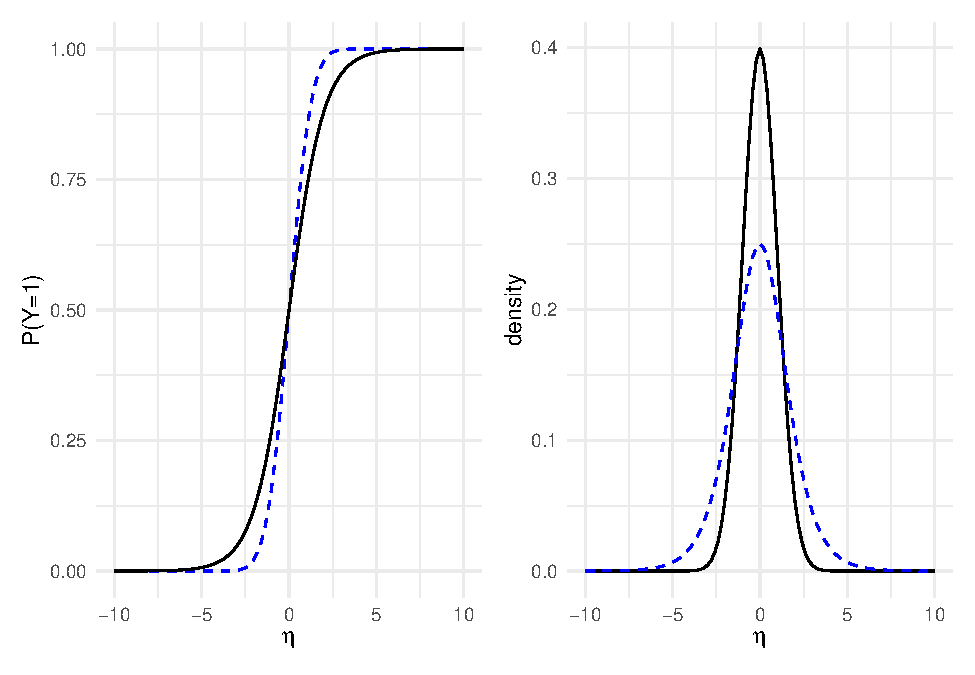
\includegraphics[width=0.7\linewidth]{MATH60604A_Statistical_modelling_files/figure-latex/probitvslogit-1} 

}

\caption{Comparison of logistic (black) and probit (dashed blue) inverse link functions (left) for binary data: both are monotone increasing functions of the linear predictor. The logistic distribution has thicker tails and thus smaller peak at zero. The right panel shows the derivative of both inverse link functions.}\label{fig:probitvslogit}
\end{figure}

The logistic regression model is nonlinear in
\(\boldsymbol{\eta}=\mathbf{X}\boldsymbol{\beta}\) and the left panel of
Figure \ref{fig:probitvslogit} shows how changes in the linear
predictor impact the probability of success. As \(\eta_i\) increases (for
example, if \(\mathrm{X}_j\) increases by one unit and \(\beta_j\) is
positive), so does the estimated probability of success because the
function \(\mathrm{expit}(x)\) is monotone increasing. This
characterization is however not helpful. If we exponentiate the linear
predictor \(\eta\), we get
\begin{align*}
\mathrm{odds}(Y\mid \mathbf{X}) =
\frac{\pi(\mathbf{X})}{1-\pi(\mathbf{X})}=\exp(\beta_0+ \beta_1
\mathrm{X}\_1 + \cdots + \beta_p\mathrm{X}\_p),
\end{align*}
where \(\pi(\mathbf{X})/\{1-\pi(\mathbf{X})\}\) are the odds of \(\mathsf{P}(Y=1 \mid \mathbf{X})\) (success) relative to \(\mathsf{P}(Y=0 \mid\mathbf{X})\) (failure). If \(\pi=0.8\), the odds are \(\pi/(1-\pi)=0.8/0.2=4\): on average, we expect four successes for one failure.

On the odds scale, the logistic regression model is multiplicative: for an increase of \(\mathrm{X}_j\) of one unit, \emph{ceteris paribus}, the odds are multiplied by \(\exp(\beta_j)\).

\begin{example}[GPA score and graduate admission]
\protect\hypertarget{exm:gpaexample}{}{\label{exm:gpaexample} \iffalse (GPA score and graduate admission) \fi{} }We consider a simple logistic model for graduate admission (yes/no) in universities across the USA as a function of their grade point average (GPA).
\end{example}

\begin{figure}

{\centering 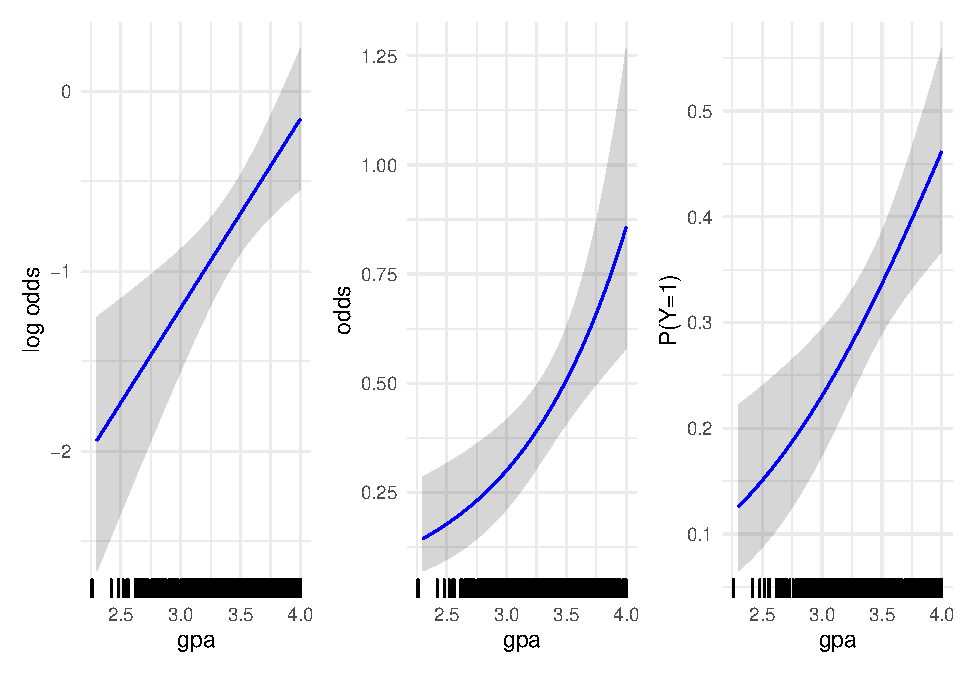
\includegraphics[width=0.7\linewidth]{MATH60604A_Statistical_modelling_files/figure-latex/figgpa-1} 

}

\caption{Graduate admission probability as a function of grade point averages (GPA) on the log odds (left), odds (middle) and probability of success scale (right). The line indicates fitted value with pointwise 95\% profile-based confidence intervals.}\label{fig:figgpa}
\end{figure}

\begin{table}

\caption{\label{tab:gpatable}Logistic regression: table of coefficients for the graduate admission data with gpa as only covariate.}
\centering
\begin{tabular}[t]{lrrrr}
\toprule
term & estimate & std. error & Wald stat. & p-value\\
\midrule
(Intercept) & -4.36 & 1.04 & -4.21 & < 0.001\\
gpa & 1.05 & 0.3 & 3.52 & < 0.001\\
\bottomrule
\end{tabular}
\end{table}

The coefficients of the simple logistic model are reported in Table \ref{tab:gpatable}, showing that the log odds of admission increase by 0.11 for each increase in GPA of \(0.1\). This translates into \(\exp(0.1\widehat{\beta}_{\mathrm{gpa}})=1.11\) on the odds ratio scale, meaning a 11\% increase in odds of admission for every \(0.1\) increase in GPA. Of course, this model is simplistic and omits other important factors\ldots{} Figure \ref{fig:figgpa} shows the variation on the log odds, odds and probability scale as a function of grade point average. While the probability scale is the most intuitive, the effect of an increase of \(0.1\) unit of GPA isn't the same, depending on what is your starting value: according to the model, the absolute increase in the probability of admission for individuals with GPA scores \(2.3\) and \(2.4\) is 1.2\%, whereas that corresponding to an increase in GPA from 3.9 to 4 is 2.6\%; this illustrates how the impact of an increase of \(0.1\) points is not the same across the board.

\begin{example}[Risk factors related to underweight babies at birth]
\protect\hypertarget{exm:birthweightex}{}{\label{exm:birthweightex} \iffalse (Risk factors related to underweight babies at birth) \fi{} }We consider a medical example related to risk factors explaining the birth weight: the birth weight is dichotomized and classified as low if the infant weight is inferior to 2.5 kg (1) and 0 otherwise. The data were collected in a medical center in Massachusetts in 1986.
\end{example}

The data contains the following explanatory variables

\begin{itemize}
\tightlist
\item
  \texttt{age}: mother's age in years.
\item
  \texttt{lwt}: mother's weight in pounds at last menstrual period.
\item
  \texttt{race}: mother's race (\texttt{white}, \texttt{black} or \texttt{other}).
\item
  \texttt{smoke}: smoking status during pregnancy (\texttt{yes}/\texttt{no}).
\item
  \texttt{ptl}: previous premature labours (\texttt{none}/\texttt{at\ least\ one}).
\item
  \texttt{ht}: history of hypertension.
\item
  \texttt{ui}: presence of uterine irritability.
\end{itemize}

\begin{figure}

{\centering 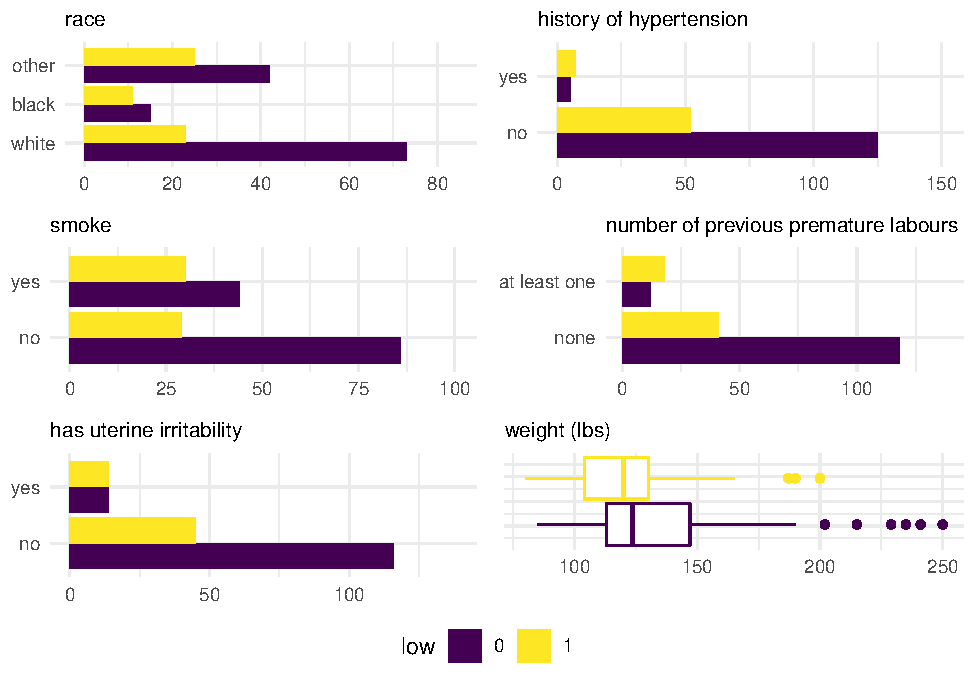
\includegraphics[width=0.7\linewidth]{MATH60604A_Statistical_modelling_files/figure-latex/birthweighteda-1} 

}

\caption{Exploratory data analysis for the birthweight data}\label{fig:birthweighteda}
\end{figure}

The exploratory data analysis suggests that smoking has a large impact, as the relative proportion of women who smoke having underweight babies is significant. Likewise, hypertension seems to bean important predictor but there are only a handful of women in the sample with this condition. Women who previously gave birth to premature babies are more likely to give birth to underweight (and potentially premature) babies, whereas women giving birth to babies under 2.5kg also typically have lower weight. We can use a logistic regression to assess the effect of these explanatories.

\begin{table}

\caption{\label{tab:logistibirthwgt}Logistic regression: table of coefficients for the birth weight data.}
\centering
\begin{tabular}[t]{lrrrr}
\toprule
term & estimate & std. error & Wald stat. & p-value\\
\midrule
(Intercept) & -0.13 & 0.97 & -0.13 & 0.9\\
mother's weight (lbs) & -0.02 & 0.01 & -2.29 & 0.022\\
race [black] & 1.3 & 0.53 & 2.46 & 0.014\\
race [other] & 0.85 & 0.44 & 1.94 & 0.053\\
smoker [yes] & 0.87 & 0.4 & 2.14 & 0.032\\
\addlinespace
previous premature labours & 1.13 & 0.45 & 2.51 & 0.012\\
hypertension [yes] & 1.87 & 0.71 & 2.64 & 0.008\\
uterine irritability & 0.75 & 0.46 & 1.64 & 0.1\\
\bottomrule
\end{tabular}
\end{table}

Table \ref{tab:logistibirthwgt} gives the estimated coefficients \(\widehat{\boldsymbol{\beta}}\) on the logs odds scale along with standard errors, Wald statistics and the \(p\)-values from the normal approximation.

We can interpret the effect of these variables: given the other variables and \emph{ceteris paribus}:

\begin{itemize}
\tightlist
\item
  the odds of giving birth to an underweight babies decrease by 1.6\% for each additional pound pre-pregnancy; this paradoxical interpretation, at odds with Figure \ref{fig:birthweighteda} is (notably) due to the correlation between smoking and mother's weight.
\item
  the odds of black women giving birth to an underweight baby are 2.67 times those of white women.
\item
  the odds of women who smoke of having a baby weighting less than 2.5kg at birth are 137.9\% higher than those of women who do not smoke.
\end{itemize}

The other parameters are interpreted accordingly. We can also check the parameter significance, by comparing the model with all the covariates and withholding one of the explanatories at the time. The results of the likelihood ratio test are presented in Table \ref{tab:type3birthwgt}.
At level 5\% and given the other factors, having previous premature labours history and uterine irritability are not statistically significant. There is no significant correlation between the explanatories, since all the variance inflation factors are inferior to \(1.5\).

\begin{table}

\caption{\label{tab:type3birthwgt}Analysis of deviance table (Type 3 decomposition) for the birthweight logistic regression model: the table gives the $p$-value for likelihood ratio tests comparing the full model including all covariates with models in which a single explanatory is removed.}
\centering
\begin{tabular}[t]{lrrr}
\toprule
variable & lik. ratio & df & p-value\\
\midrule
mother's weight & 5.96 & 1 & 0.015\\
race & 7.61 & 2 & 0.022\\
smoker & 4.72 & 1 & 0.03\\
previous premature labours & 6.37 & 1 & 0.012\\
hypertension & 7.31 & 1 & 0.007\\
\addlinespace
uterine irritability & 2.63 & 1 & 0.1\\
\bottomrule
\end{tabular}
\end{table}

\hypertarget{issues-with-binary-data}{%
\subsection{Issues with binary data}\label{issues-with-binary-data}}

One oddity of regression models for binary data is that most of the
information in the sample is provided by response whose variance is
largest (points that have \(\pi\) far from 0 or 1). This can be seen by
looking at how the probability \(\pi\) changes as a function of changes in
the \(j\)th explanatory \(\mathrm{X}_j\): if
\(\pi = \mathrm{expit}(\beta_0 + \beta_1\mathrm{X}_1 + \cdots + \beta_p\mathrm{X}_p)\),
then \(\partial \pi/\partial \mathrm{X}_j = \beta_j \pi(1-\pi)\), so the
effect of \(\beta_j\) is large when \(\pi\) is near \(0.5\) and near zero if
the probabilities are close to the endpoints \(0\) or \(1\). Thus, if one
wants to estimate a coefficient \(\beta_j\) of large magnitude, the ratio
\(|\beta_j|/\mathsf{sd}(\beta_j) \to 0\) as \(\beta_j \to \infty\): the
power for testing that \(\beta_j=0\) using a Wald statistic tends to zero.
Wald statistics are not recommended for Bernoulli data: the following
simple example illustrates why.

\begin{example}[Incoherent results for Wald tests]
\protect\hypertarget{exm:waldgarbage}{}{\label{exm:waldgarbage} \iffalse (Incoherent results for Wald tests) \fi{} }Suppose we consider a simple binary model and \(n=100\) observations and the null hypothesis \(\mathscr{H}_0:\pi = 0.5\) and equivalently for the logistic model \(Y_i \sim \mathsf{Bin}\{m, \mathrm{expit}(\beta_0)\}\), where this same hypothesis amounts to \(\mathscr{H}_0:\beta_0=0\). Figure \ref{fig:WaldgarbageR} clearly shows that lack of invariance of the Wald statistic to reparametrization. When \(\widehat{\beta}_0\) increases and \(m\) is large, the Wald statistic for \(\beta_0\) decreases as we approach \(m\) successes, because the standard error of \(\widehat{\beta}_0\) increases faster than the difference \(\widehat{\beta}-0\). Both statistics are asymptotically normal if the null hypothesis holds true, so the two-sided test would reject if the value of the Wald statistic is greater than 1.96. Depending on the parametrization, however, they give different results: the statistic increases monotonically for \(\pi\), but would converge to zero for \(\beta_0\) when \(m\) is large (allowing thereby larger values of \(\widehat{\beta}_0\)). No such problem arises when considering score and likelihood ratio tests.
\end{example}

\begin{figure}

{\centering 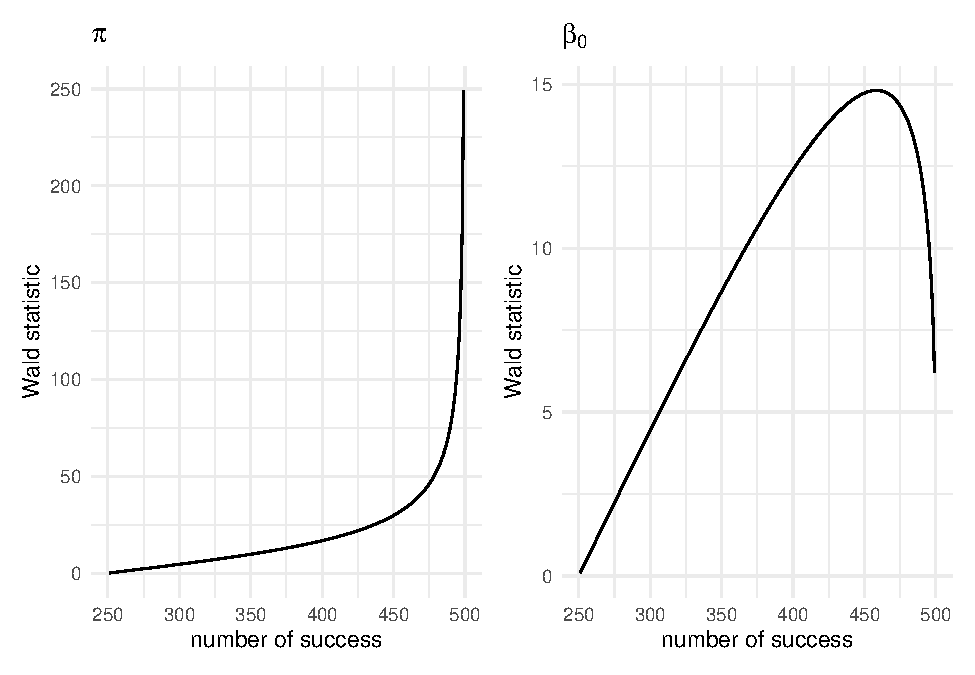
\includegraphics[width=0.7\linewidth]{MATH60604A_Statistical_modelling_files/figure-latex/WaldgarbageR-1} 

}

\caption{Wald test statistic for $Y_i \sim \mathsf{Bin}(m=500, \pi)$ (left)  for $\pi=0.5$ and the same hypothesis test on the logistic scale with $Y_i \sim \mathsf{Bin}(m=500, \mathrm{expit}(\beta_0))$ and $\mathscr{H}_0:\beta_0=0$ (right) as a function of the number of success out of 500 trials.}\label{fig:WaldgarbageR}
\end{figure}

Thus, information about the coefficients only accumulates if the true
regression coefficients \(\boldsymbol{\beta}\) are small. The deviance and
Pearson provide little to no information about the quality of the model
adjustment and their null distribution depends on
\(\widehat{\boldsymbol{\beta}}\): with large coefficients, the asymptotic
\(\chi^2\) distribution is not a good approximation and relying on these
to determine goodness-of-fit is not recommended.

\hypertarget{quasi-separation-of-variables}{%
\subsection{Quasi-separation of variables}\label{quasi-separation-of-variables}}

One common problem with binary data is the problem of complete
separation of variables: in this scenario, a linear combination of the
explanatories allows to perfectly categorize \(Y_i\) into \(0/1\) depending
on the value of the covariates and the predicted probabilities will be
exactly zero or one. While this is not a problem for prediction, the
coefficients that yield such a sharp transition are near infinite, as
displayed in Figure \ref{fig:sepvarplot}; software may or not pick up
such error, but in any case Wald tests for individual coefficients are
rubbish. This is problematic for inference because we cannot
meaningfully interpret the resulting parameters.

\begin{table}
\caption{\label{tab:quasisepvar}Logistic regression: simulated dataset exhibiting separation of variables with standard logistic model (left) and Firth's regression (right). The large coefficients and standard errors, combined with near zero residuals, are all indicative of separation of variable.}

\centering
\begin{tabular}[t]{lrr}
\toprule
term & estimate & std. error\\
\midrule
(Intercept) & -829 & 311291\\
x & 92.5 & 34781\\
\bottomrule
\end{tabular}
\centering
\begin{tabular}[t]{lr}
\toprule
estimate & std. error\\
\midrule
-5.6 & 2.8\\
0.6 & 0.3\\
\bottomrule
\end{tabular}
\end{table}

Inspection of the coefficients and their standard errors is a good way to detect such problems: parameters that are large (with standardized explanatories with mean zero variance one inputs) with \(|\widehat{\beta}_j| > 36\) are particularly suspicious; the number of iterations for the optimization routine is also often abnormally large. While the Wald statistic for \(\beta_1=0\) is nearly zero and the \(p\)-value 1, the likelihood ratio test yields a statistic of 20.016 with a negligible associated \(p\)-value.

One way to restore finiteness of the \(\boldsymbol{\beta}\) is to impose a penalty term that prevents near infinite parameter values. Firth's penalty is the most popular solution (option \texttt{firth} in the \textbf{SAS} procedure \texttt{logistic} and \texttt{logistf::logistf} function in \textbf{R}.

\begin{figure}

{\centering 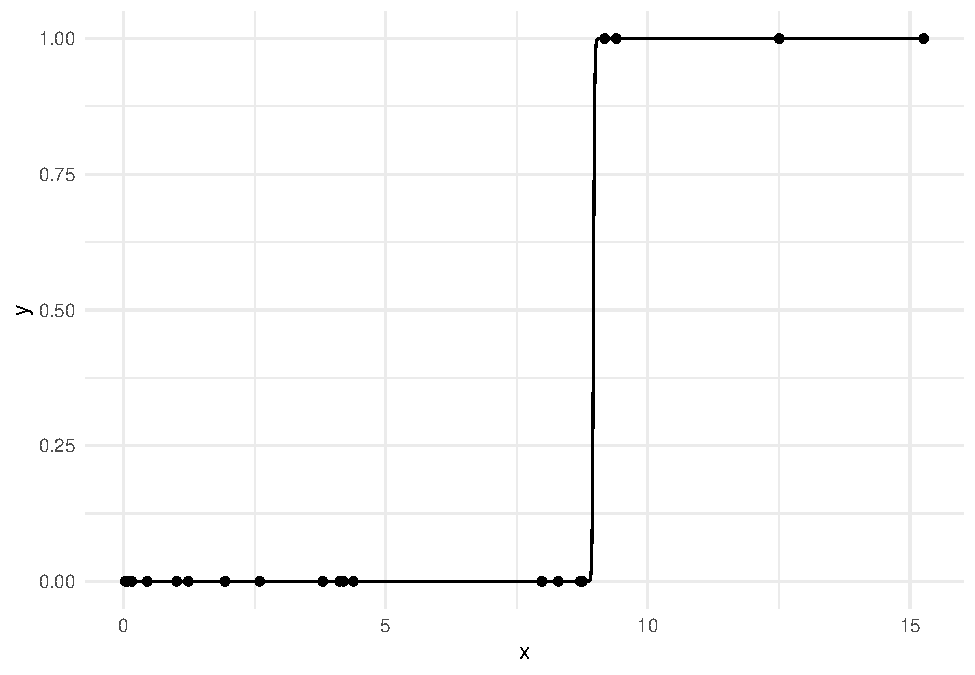
\includegraphics[width=0.7\linewidth]{MATH60604A_Statistical_modelling_files/figure-latex/sepvarplot-1} 

}

\caption{Illustration of complete separation of variable on simulated observations. Parameters are near infinite to yield a sharp transition at $x=9$. Quasi-complete separation of variable occurs if both outcomes are observed at the cutoff point.}\label{fig:sepvarplot}
\end{figure}

\hypertarget{diagnostic-plots-for-binary-data-star}{%
\subsection{\texorpdfstring{Diagnostic plots for binary data (\(\star\))}{Diagnostic plots for binary data (\textbackslash star)}}\label{diagnostic-plots-for-binary-data-star}}

There are also other issues arising from the discreteness of the
observations. Since observations are 0/1, residuals are often separated.
Figure \ref{fig:diagplotsbirthwt1} shows residual plots for Example
\ref{exm:birthweightex}: both plots are of limited use to assess
goodness-of-fit and model assumptions.

\begin{figure}

{\centering 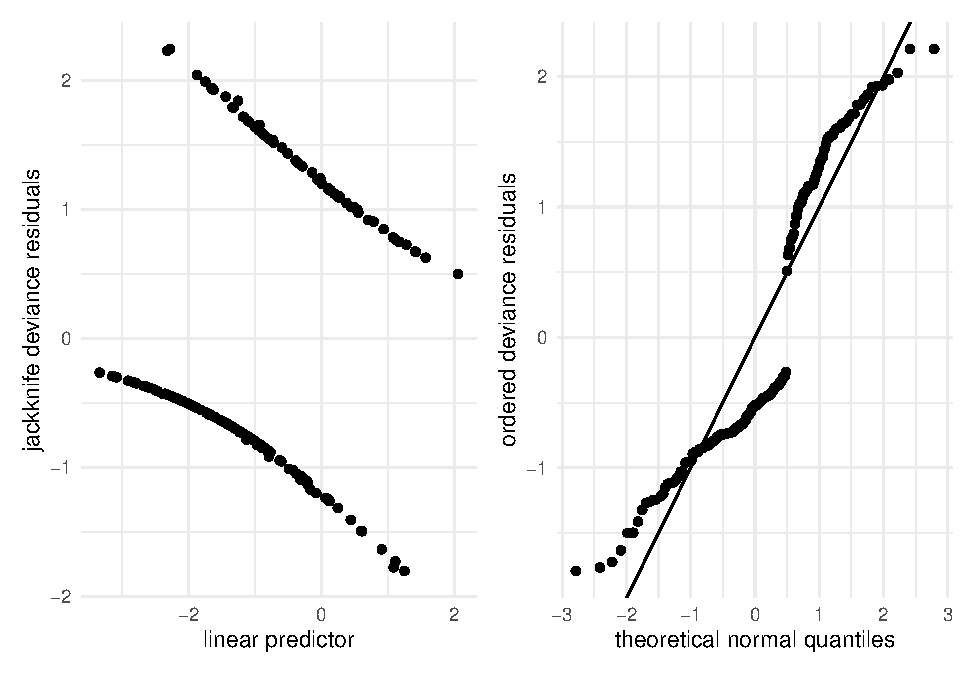
\includegraphics[width=0.7\linewidth]{MATH60604A_Statistical_modelling_files/figure-latex/diagplotsbirthwt1-1} 

}

\caption{Diagnostic plots for the binary regression for the birth weight data: jackknife deviance residuals against linear predictor (left) and quantile-quantile plot of ordered deviance residuals (right).}\label{fig:diagplotsbirthwt1}
\end{figure}

Another strategy is use of quantile residuals
\citep{Brillinger/Preisler:1983}. If \(Y \sim F\), the quantile transform gives \(U=F(Y) \sim \mathsf{U}(0,1)\), meaning uniformly distributed on \((0,1)\). Replacing the unknown distribution \(F\) by \(\widehat{F}\) should yield approximately uniform observations. With \(\widehat{\pi}_i\) denoting the probability of success, we take
\begin{align*}
U_i = U_{i1} Y_i + U_{i2}(1-Y_i), \qquad U_{i1} \sim \mathsf{U}(0, \widehat{\pi}_i), \quad U_{i2} \sim \mathsf{U}(\widehat{\pi}_i, 1)
\end{align*}
and the resulting \textbf{uniform residuals} will be, as their name hints, approximately uniform on \((0,1)\). The drawback of this approach lies in the randomness of the residuals. Figure \ref{fig:diagplotbirthwgt} shows the diagnostic plots based on the uniform residuals (top two rows): there is no overall indication of poor fit, except for seemingly too few low/high residuals. The two observations with high leverage correspond to non-smoker mothers with no premature labour record: one with hypertension and a weight of 95lbs (unusual combination), the other weighting 200 lbs, with no hypertension and presence of uterine
irritability.

\begin{figure}

{\centering 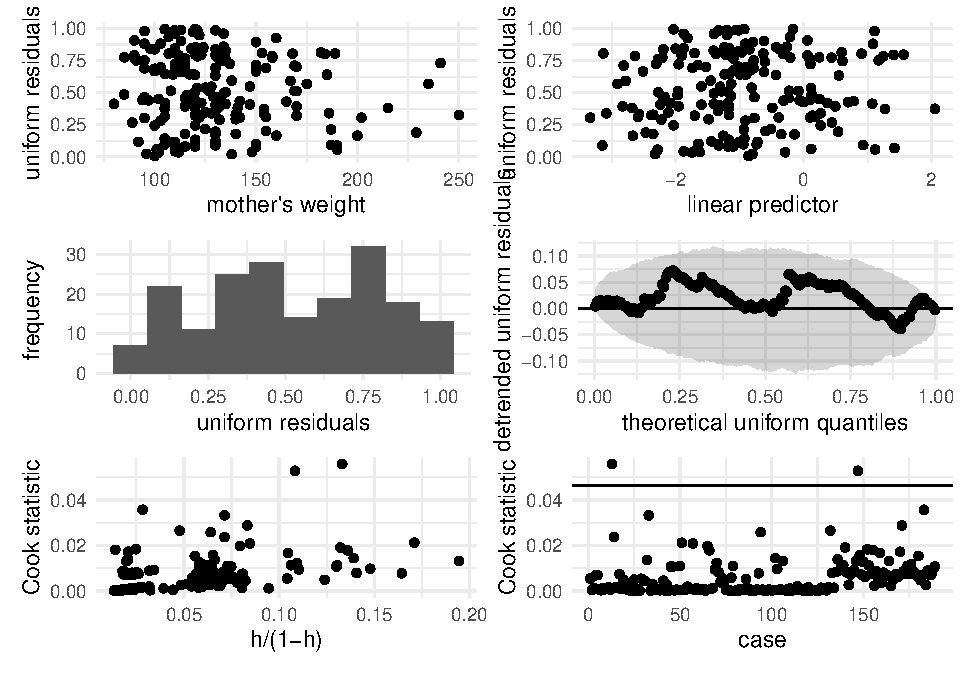
\includegraphics[width=0.7\linewidth]{MATH60604A_Statistical_modelling_files/figure-latex/diagplotbirthwgt-1} 

}

\caption{Diagnostic plots based on uniform residuals for the birth weight data. From left to right, top to bottom: residuals against explanatory and linear predictors, histogram of uniform residuals and Tukey's quantile-quantile plot, Cook statistic against weighted leverage and case number. }\label{fig:diagplotbirthwgt}
\end{figure}

\hypertarget{count-data}{%
\section{Count data}\label{count-data}}

If a response is integer value, the linear model is seldom appropriate because the variable is skewed, which even the log-linear model may fail to capture. It may thus be appropriate to look at generalized linear models for discrete data.

The most widespread model for count data is the Poisson regression. The Poisson distribution arises as the limit of binomial data with a small probability of success as the number of attempts becomes large: examples include rare medical conditions, number of accidents, or goals in a soccer (football) match. The mean and variance of the Poisson distribution are both \(\lambda\), so the model imposes stringent constraints on the observations. Extensions that deal with zero-inflation, underdispersed and overdispersed data are widespread. Most count data are found in contingency tables, in which the cells give the counts, while the dimensions of the table represent categorical variables. Such data format are convenient for storage and display, but must be transformed to long format for model fitting.

The canonical link of the Poisson model is the natural logarithm \(\ln(x)\) and the interpretation will be similar to that of the \href{transformation-response}{log-linear model}. Specifically, suppose the
mean model is
\begin{align*}
\mu = \exp(\beta_0 + \beta_1 \mathrm{X}_{1} + \cdots + \beta_p \mathrm{X}_{p}),
\end{align*}
so the mean is multiplied by \(\exp(\beta_j)\) for an increase of one unit of \(\mathrm{X}_{j}\), \emph{ceteris paribus}. If \(\beta_j < 0\), \(\exp(\beta_j) < 1\) and so we have a decrease of \(100\cdot(1-\exp(\beta_j))\)\% of the mean response. Likewise, if \(\beta_j>0\), the mean number increases by \(100\cdot(\exp(\beta_j)-1)\)\%. The interpretation of interactions between categorical and continuous/categorical variables is similar to that of multiplicative (log-linear) models.

\begin{example}[Road accidents and speed limits on the motorway in Sweden]
\protect\hypertarget{exm:roadsweden}{}{\label{exm:roadsweden} \iffalse (Road accidents and speed limits on the motorway in Sweden) \fi{} }Sweden is a worlwide leader in road safety and has a long history of countermeasures to increase road traffic safety, including the Vision Zero program. Back in the 1960s, a study was conducted by the authorities to investigate the potential of speed limits on motorways to reduce the number of accidents. The \texttt{sweden} data contains the number of accidents on 92 matching days in both 1961 and 1962 \citep{Svensson:1981}; speed limits were in place on selected days in either year.
\end{example}

We consider an example from Section 4.5 of \citet{Brazzale/Davison/Reid:2007}.
To study the impact of the restrictions we can fit a Poisson model. Let
\(Y_{i1}\) (respectively \(Y_{i2}\)) denote the number of accidents in 1961
(1962) on day \(i\) and let \(\texttt{limit}_{ij}\) denote a binary
indicator equal to one if speed limits were enforced on day \(i\) of year
\(j\). We set
\begin{align*}
Y_{i1} \sim \mathsf{Po}(\delta_i + \alpha \texttt{limit}_{i1}), \quad Y_{i2} \sim\mathsf{Po}(\delta_i + \gamma +  \alpha \texttt{limit}_{i2}), \qquad i=1, \ldots, 92. 
\end{align*}
The nuisance parameters \(\delta_1, \ldots, \delta_{92}\) control for changes in background number of accidents and are of no practical interest, while \(\gamma\) denotes the change from 1961 to 1962. We are interested here in assessing changes in the number of accidents due to the policy, \(\alpha\); of secondary interest is to determine whether there has been a decrease in the number of accident relative to 1961.

\begin{table}

\caption{\label{tab:swedenglm}Analysis of deviance table (Type 3 decomposition) for the Poisson regression model fitted to the Sweden traffic restrictions data: the table gives the $p$-value for likelihood ratio tests comparing the full model including all covariates with models in which a single explanatory is removed.}
\centering
\begin{tabular}[t]{lrrr}
\toprule
variable & lik. ratio & df & p-value\\
\midrule
day & 9395.22 & 92 & < 0.001\\
limit & 46.29 & 1 & < 0.001\\
year & 0.7 & 1 & 0.4\\
\bottomrule
\end{tabular}
\end{table}

The residual deviance is 107.95 for 90 degrees of freedom, suggests the overall fit is good, despite the large number of nuisance parameters \(\delta_1, \ldots, \delta_{92}\). The coefficient associated to limit is strongly significant: the estimated coefficient is \(\widehat{\alpha}=-0.292\), indicates that speed limits reduce the mean number of accidents by \(25.3\)\% on average. In contrast, the likelihood ratio test reported in Table \ref{tab:swedenglm} shows that the change in the yearly number of accident from 1961 to 1962, \(\gamma\), is not significantly different from zero.

\hypertarget{overdispersion}{%
\subsection{Overdispersion}\label{overdispersion}}

One restriction of the Poisson model is that the restriction on its moments is often unrealistic. We tackle the problem of \textbf{overdispersion}, for which the variability in the counts is larger than that implied by a Poisson distribution.

Overdispersion is not the only problem encountered in practice: sometimes, the variance is smaller than the mean, typically due to excess of zeros. Hurdle models and zero-inflated models can be used to deal with this issue. The most common framework for handling overdispersion is to consider that the mean \(\lambda\) of the Poisson distribution is itself a positive random variable with mean \(\mu\). By the laws of iterated expectation and iterative variance,
\begin{align*}
\mathsf{E}(Y) &= \mathsf{E}_{\Lambda}\{\mathsf{E}(Y \mid \Lambda\} = \mathsf{E}(\Lambda) = \mu\\
\mathsf{Va}(Y) &= \mathsf{E}_{\Lambda}\{\mathsf{Va}(Y \mid \Lambda)\} + \mathsf{Va}_{\Lambda}\{\mathsf{E}(Y \mid \Lambda)\} = \mathsf{E}(\Lambda) + \mathsf{Va}(\Lambda) = \mu + \mathsf{Va}(\Lambda).
\end{align*}
This hierarchical model thus necessarily yield a model in which the variance is higher than the mean. If \(\Lambda\) follows a \href{https://en.wikipedia.org/wiki/Gamma_distribution}{gamma distribution} with scale \(k\mu\) and rate \(k>0\), \(\Lambda \sim \mathsf{Ga}(k\mu, k)\). This yields a marginal distribution for the response \(Y\) which follows a negative binomial distribution, whose mean and variance are
\begin{align*}
\mathsf{E}(Y) = \mu, \qquad \mathsf{Va}(Y) = \mu + k \mu^2.
\end{align*}
The term \(k\) is a dispersion parameter, which is fixed for all observations. As \(k \to 0\), the distribution of \(\Lambda\) degenerates to a constant at \(\mu\) and we recover th e Poisson model. While both negative binomial and Poisson models are nested, the likelihood ratio test is non-regular because the restriction we test lies on the boundary of the parameter space, as \(k \in (0, \infty)\). The consequence is that, in large samples, if the data are truly Poisson and we fit a negative binomial, we expect the maximum likelihood estimator of the dispersion parameter \(k\) to be exactly zero half of the time and
to be positive and behave like a \(\chi_1^2\) random variable the other half of the time.

Strictly speaking, the negative binomial expansion presented above is not a generalized linear model unless \(k\) is known, but we can write down the log-likelihood and fit the model by alternating maximization of \(\boldsymbol{\beta}\) and \(k\) and perform likelihood-based inference as usual.

\begin{example}
\protect\hypertarget{exm:unnamed-chunk-2}{}{\label{exm:unnamed-chunk-2} }We can ascertain the finite sample properties of the likelihood ratio test by simulating repeatedly from a Poisson regression model, fitting the negative binomial model and calculating the likelihood ratio statistic. Since the negative binomial model yields \(k>0\), we include \(k=0\) by fitting a Poisson model and keeping the latter whenever it yields a higher log likelihood than the one found by maximizing the negative binomial model.
\end{example}

\begin{figure}

{\centering 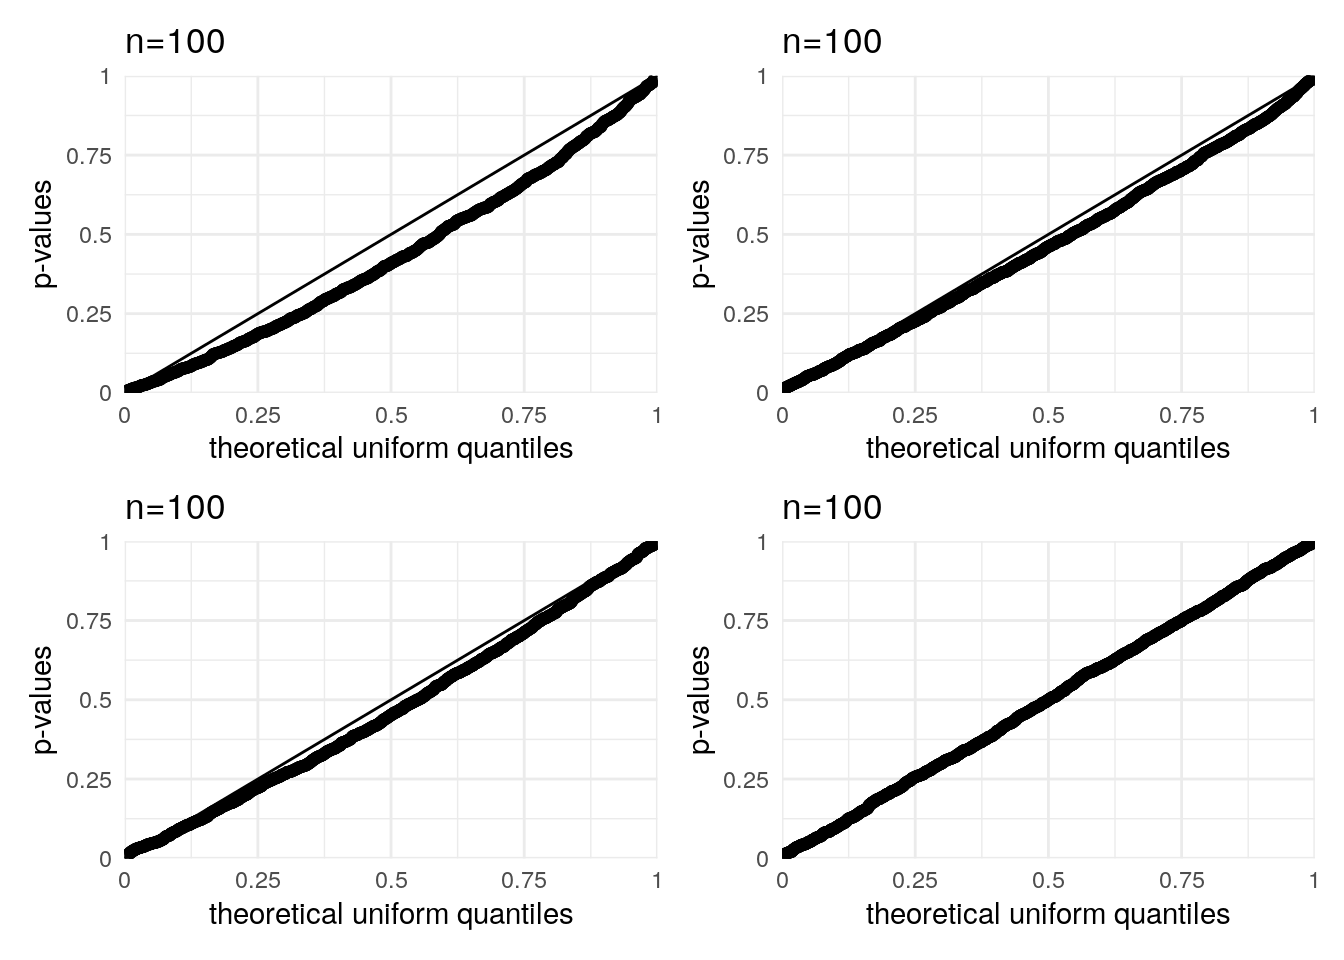
\includegraphics[width=0.7\linewidth]{MATH60604A_Statistical_modelling_files/figure-latex/simunb-1} 

}

\caption{Simulated null distribution of the likelihood ratio test comparing the Poisson and negative binomial regression models. The quantile-quantile plot show the distribution of positive statistics for sizes $n=100, 500, 1000, 2000$ relative to the asymptotic $\frac{1}{2}\chi^2_1$.}\label{fig:simunb}
\end{figure}

The percentage of likelihood ratio statistics that are zero is \(69\)\%, \(60\)\%, \(59\)\% and \(54\)\% for respectively \(n=100\), \(500\), \(1000\) and \(2000\). We can also see from the quantile-quantile plots that the empirical distribution of the positive values is right skewed relative to the \(\chi^2_1\) reference. This strongly suggest that asymptotic null distribution, consisting of a point mass with probability half at \(0\) and \(\chi^2_1\) with probability half is seemingly valid only for very large samples; bear in mind that these findings also don't account for model misspecification.

\hypertarget{modelling-proportions}{%
\section{Modelling proportions}\label{modelling-proportions}}

Proportions arise when we condition on the total number of observations for a scenario. With Poisson counts, this gives rise to a multinomial distribution for the proportions. We can also consider counts as the fraction of total population, including the total population if counts are not comparable using an offset term.

For the first instance, we can consider \(D\) individual counts as Poisson. There is a direct link with (multinomial) logistic model: if we condition on the sum of the counts, we recover a multinomial distribution; for simplicity, we restrict attention to the binomial case when \(D=2\).

Consider independent Poisson counts \(Y_1, Y_2\) with respective means \(\lambda_1, \lambda_2\). Suppose the total counts \(Y_1 + Y_2 = m\).
The distribution of \(Y_2 \mid Y_1 + Y_2=m \sim \mathsf{Bin}\{m, \lambda_2/(\lambda_1 + \lambda_2)\}\).
If we model each mean parameter as, \(\ln(\lambda_i) = \alpha + \mathbf{x}_i^\top\boldsymbol{\beta}\) where \(\mathbf{x}_i\) is a \(p\) row vector, then
\begin{align*}
\frac{\lambda_2}{\lambda_1 + \lambda_2} = \frac{\exp\{(\mathbf{x}_2-\mathbf{x}_1)^\top\boldsymbol{\beta}\}}{1+\exp\{(\mathbf{x}_2-\mathbf{x}_1)^\top\boldsymbol{\beta}\}}.
\end{align*}
We could thus estimate \(\boldsymbol{\beta}\) using a logistic regression, but the common intercept \(\alpha\) that appears in the mean of the Poisson counts is not estimable based on this conditional likelihood.

\begin{example}
\protect\hypertarget{exm:swedenex2}{}{\label{exm:swedenex2} }
Looking again at the data in Example \ref{exm:roadsweden}, we condition on the sum of the number of accidents in 1961 and 1962, \(Y_{i1} + Y_{i2}\), and adjust the same mean model for the Poisson data.
\end{example}
Recall
\begin{align*}
\frac{\lambda_{i2}}{
\lambda_{i1} + \lambda_{i2}} &= \frac{\exp(\delta_i + \gamma + \alpha \texttt{limit}_{i2})}{(\exp(\delta_i + \gamma + \alpha \texttt{limit}_{i2}) + \exp(\delta_i + \alpha \texttt{limit}_{i1})} \\&= \frac{\exp\{\gamma + \alpha(\texttt{limit}_{i2}-\texttt{limit}_{i1})\}}{1+{\exp\{\gamma + \alpha(\texttt{limit}_{i2}-\texttt{limit}_{i1})\}}}, \qquad i=1, \ldots, 92. 
\end{align*}

In this case, we were not interested in the nuisance parameters \(\delta_1, \ldots, \delta_{92}\), which were there merely for the sake of controlling for daily changes. The binomial logistic model has only two parameters, but 92 observations rather than 184 since we regroup the counts.
The parameter estimates (standard errors) based on the logistic regression are \(\widehat{\alpha} = -0.292 (0.043)\) and \(\widehat{\gamma}=-0.029(0.035)\), so enforcing a speed limit reduces the accident rate by \(\exp(-0.292)=0.75\), corresponding to a 25\% decrease. The 95\% profile likelihood confidence interval for this reduction, \(\exp(\alpha)\), is \([0.60, 0.81]\), and there are thus strong evidence that the reduction in the number of accident is real. The confidence interval for \(\gamma\), on the other hand, is \([-0.097, 0.039]\) includes zero; the yearly change is not significative. Since the inference are exactly the same, one may wonder what the benefit of using the logistic model is; it mostly lies in the fact our model has 2 parameters and not 94\ldots{}

We present an example of incorrect marginalization that leads to Simpson's paradox. Models for multi-way contingency tables and proportions are covered in a dedicated section.

\hypertarget{simpsons-paradox}{%
\subsection{Simpson's paradox}\label{simpsons-paradox}}

\hypertarget{correlated-longitudinal-data}{%
\chapter{Correlated and longitudinal data}\label{correlated-longitudinal-data}}

\hypertarget{linear-mixed-models}{%
\chapter{Linear mixed models}\label{linear-mixed-models}}

\hypertarget{survival}{%
\chapter{Survival analysis}\label{survival}}

\hypertarget{appendix-appendix}{%
\appendix}


\hypertarget{complement}{%
\chapter{Complements}\label{complement}}

\hypertarget{population-sample}{%
\section{Population and samples}\label{population-sample}}

Statistics is the science of uncertainty quantification: of paramount importance is the notion of randomness. Generally, we will seek to estimate characteristics of a population using only a sample (a sub-group of the population of smaller size).

The \textbf{population of interest} is a collection of individuals which the study targets. For example, the Labour Force Survey (LFS) is a monthly study conducted by Statistics Canada, who define the target population as ``all members of the selected household who are 15 years old and older, whether they work or not.'' Asking every Canadian meeting this definition would be costly and the process would be long: the characteristic of interest (employment) is also a snapshot in time and can vary when the person leaves a job, enters the job market or become unemployed.

In general, we therefore consider only \textbf{samples} to gather the information we seek to obtain. The purpose of \textbf{statistical inference} is to draw conclusions about the population, but using only a share of the latter and accounting for sources of variability. George Gallup made this great analogy between sample and population:

\begin{quote}
One spoonful can reflect the taste of the whole pot, if the soup is well-stirred
\end{quote}

A \textbf{sample} is a random sub-group of individuals drawn from the population. Creation of sampling plans is a complex subject and semester-long sampling courses would be required to evens scratch the surface of the topic. Even if we won't be collecting data, keep in mind the following information: for a sample to be good, it must be representative of the population under study. Selection bias must be avoided, notably samples of friends or of people sharing opinions.

Because the individuals are selected at \textbf{random} to be part of the sample, the measurement of the characteristic of interest will also be random and change from one sample to the next. However, larger samples of the same quality carry more information and our estimator will be more precise. Sample size is not guarantee of quality, as the following example demonstrates.

\begin{example}
\protect\hypertarget{exm:Galluppoll}{}{\label{exm:Galluppoll} }
\emph{The Literary Digest} surveyed 10 millions people by mail to know voting preferences for the 1936 USA Presidential Election. A sizeable share, 2.4 millions answered, giving Alf Landon (57\%) over incumbent President Franklin D. Roosevelt (43\%). The latter nevertheless won in a landslide election with 62\% of votes cast, a 19\% forecast error. \href{https://www.jstor.org/stable/2749114}{Biased sampling and differential non-response are mostly responsible for the error:} the sampling frame was built using ``phone number directories, drivers' registrations, club memberships, etc.'\,', all of which skewed the sample towards rich upper class white people more susceptible to vote for the GOP.

In contrast, Gallup correctly predicted the outcome by polling (only) 50K inhabitants. \href{https://medium.com/@ozanozbey/how-not-to-sample-11579793dac}{Read the full story here.}
\end{example}

\hypertarget{random-variable}{%
\section{Random variable}\label{random-variable}}

Suppose we wish to describe the behaviour of a stochastic phenomenon. To this effect, one should enumerate the set of possible values taken by the variable of interest and their probability: this is what is encoded in the distribution. We will distinguish between two cases: discrete and continuous variables. Random variables are denoted using capital letters: for example \(Y \sim \mathsf{No}(\mu, \sigma^2)\) indicates that \(Y\) follows a normal distribution with parameters \(\mu\) and \(\sigma^2\), which represent respectively the expectation and variance of \(Y\).

The (cumulative) distribution function \(F(y)\) gives the cumulative probability that an event doesn't exceed a given numerical value \(y\), \(F(y) = \mathsf{Pr}(Y \leq y)\).

If \(Y\) is discrete, then it has atoms of non-zero probability and the mass function \(f(y)=\mathsf{Pr}(Y=y)\) gives the probability of each outcome \(y\). In the continuous case, no numerical value has non-zero probability and so we consider intervals instead: the density function gives the probability of \(Y\) falling in a set \(B\), via \(\mathsf{Pr}(Y \in B) = \int_B f(y) \mathrm{d} y\). It follows that the distribution function of a continuous random variable is simply \(F(y) = \int_{-\infty}^y f(x) \mathrm{d} x\).

\begin{figure}

{\centering \includegraphics[width=0.7\linewidth]{images/02-ttest-DF_illustration} 

}

\caption{(Cumulative) distribution functions (top) and density/mass functions (bottom) of continuous (left) and discrete (right) random variables.}\label{fig:distributions}
\end{figure}

\hypertarget{moments}{%
\subsection{Moments}\label{moments}}

One of the first topics covered in introductory statistics is descriptive statistics such as the mean and standard deviation. These are estimators of (centered) moments, which characterise a random varaible. In the case of the standard normal distribution, the expectation and variance fully characterize the distribution.

Let \(Y\) be a random variable with density (or mass) function \(f(x)\). This function is non-negative and satisfies \(\int_{\mathbb{R}} f(x) \mathrm{d}x=1\): the integral over a set \(B\) gives the probability of \(Y\) falling inside \(B \in \mathbb{R}\).

The expectation (or theoretical mean) of a continuous random variable \(Y\) is \[\mathsf{E}(Y)=\int_{\mathbb{R}} x f(x) \mathrm{d} x.\]
In the discrete case, we set rather \(\mu = \mathsf{E}(Y)=\sum_{x \in \mathcal{X}} x \mathsf{Pr}(X=x)\), where \(\mathcal{X}\) denotes the support of \(Y\), the set of numerical values at which the probability of \(Y\) is non-zero.
More generally, we can look at the expectation of a function \(g(x)\) for \(Y\), which is nothing but the integral (or sum in the discrete case) of \(g(x)\) weighted by the density or mass function of \(f(x)\). In the same fashion, provided the integral is finite, the variance is
\[\mathsf{Va}(Y)=\mathsf{E}\{Y-\mathsf{E}(Y)\}^2 \equiv \int_{\mathbb{R}} (x-\mu)^2 f(x) \mathrm{d} x.\]
The \textbf{standard deviation} is the square root of the variance and measures the variability of the variable, measured in the same units as \(Y\).

The notion of moments can be extended to higher dimensions. If we assume data are independent, their joint distribution factorizes into the product of the individual mass function/density of each sample point. Otherwise, a multivariate mass function or density function describes the behaviour of the random vector.

Consider an \(n\)-vector \(\boldsymbol{Y}\). In the regression setting, the response \(\boldsymbol{Y}\) would usually comprise repeated measures on an individual, or even observations from a group of individuals.

The expected value (theoretical mean) of the vector \(\boldsymbol{Y}\) is calculated componentwise, i.e.,
\begin{align*}
\mathsf{E}(\boldsymbol{Y}) &= \boldsymbol{\mu}=
\begin{pmatrix}
\mathsf{E}(Y_1) &
\cdots  &
\mathsf{E}(Y_n)
\end{pmatrix}^\top
\end{align*}
whereas the second moment of \(\boldsymbol{Y}\) is encoded in the \(n \times n\) \textbf{covariance} matrix
\begin{align*}
\mathsf{Va}(\boldsymbol{Y}) &= \boldsymbol{\Sigma} = \begin{pmatrix} \mathsf{Va}(Y_1) & \mathsf{Co}(Y_1, Y_2)  & \cdots & \mathsf{Co}(Y_1, Y_n) \\
\mathsf{Co}(Y_2, Y_1) & \mathsf{Va}(Y_2) & \ddots & \vdots \\
\vdots & \ddots & \ddots & \vdots \\
\mathsf{Co}(Y_n, Y_1) & \mathsf{Co}(Y_n, Y_2) &\cdots & \mathsf{Va}(Y_n)
\end{pmatrix}
\end{align*}
The \(i\)th diagonal element of \(\boldsymbol{\Sigma}\), \(\sigma_{ii}=\sigma_i^2\), is the variance of \(Y_i\), whereas the off-diagonal entries \(\sigma_{ij}=\sigma_{ji}\) \((i \neq j)\) are the covariance of pairwise entries, with
\begin{align*}
\mathsf{Co}(Y_i, Y_j) = \int_{\mathbb{R}^2} (y_i-\mu_i)(y_j-\mu_j) f_{Y_i, Y_j}(y_i, y_j) \mathrm{d} y_i \mathrm{d} y_j.
\end{align*}
The covariance matrix \(\boldsymbol{\Sigma}\) is thus symmetric. It is customary to normalize the pairwise dependence so they do not depend on the component variance. The linear \textbf{correlation} between \(Y_i\) and \(Y_j\) is
\begin{align*}
\rho_{ij}=\mathsf{Cor}(Y_i,Y_j)=\frac{\mathsf{Co}(Y_i, Y_j)}{\sqrt{\mathsf{Va}(Y_i)}\sqrt{\mathsf{Va}(Y_j)}}=\frac{\sigma_{ij}}{\sigma_i\sigma_j}.
\end{align*}
The correlation matrix of \(\boldsymbol{Y}\) is an
\(n\times n\) symmetric matrix with ones on the diagonal and the pairwise correlations off the diagonal,
\begin{align*}
\mathsf{Cor}(\boldsymbol{Y})=
\begin{pmatrix}
1 & \rho_{12} & \rho_{13} & \cdots & \rho_{1n}\\
\rho_{21} & 1 & \rho_{23} & \cdots & \rho_{2n} \\
\rho_{31} & \rho_{32} & 1 & \ddots & \rho_{3n} \\
\vdots & \vdots & \ddots & \ddots & \vdots \\
\rho_{n1} & \rho_{n2} & \rho_{n3} & \cdots & 1
\end{pmatrix}.
\end{align*}
One of the most important parts of modelling
correlated (or longitudinal) data is the need to account for within-group correlations. This basically comes down to modelling a covariance matrix for observations within the same group (or within the same individual in the case of repeated measures), which is the object of \href{correlated-longitudinal-data}{Chapter 5}.

\hypertarget{unbiasedness-and-mean-square-error}{%
\subsection{Unbiasedness and mean square error}\label{unbiasedness-and-mean-square-error}}

An estimator \(\hat{\theta}\) for a parameter \(\theta\) is unbiased if its bias \(\mathsf{bias}(\hat{\theta})=\mathsf{E}(\hat{\theta})- \theta\) is zero.
The unbiased estimator of the mean and the variance of \(Y\) are
\begin{align*}
\overline{Y}_n &= n^{-1} \sum_{i=1}^n Y_i\\
S_n &= (n-1)^{-1} \sum_{i=1}^n (Y_i-\overline{Y})^2.
\end{align*}
While unbiasedness is a desirable property, there may be cases where no unbiased estimator exists for a parameter! Often, rather, we seek to balance bias and variance: recall that an estimator is a function of random variables and thus it is itself random: even if it is unbiased, the numerical value obtained will vary from one sample to the next. We often seek an estimator that minimises the mean squared error, \[\mathsf{MSE}(\hat{\theta}) = \mathsf{E}\{(\hat{\theta}-\theta)^2\}=\mathsf{Va}(\hat{\theta}) + \{\mathsf{E}(\hat{\theta})\}^2.\]
The mean squared error is an objective function consisting of the sum of the squared bias and the variance.

An alternative to this criterion is to optimize a function such as the likelihood of the sample: the resulting estimator is termed maximum likelihood estimator. These estimator are asymptotically efficient, in the sense that they have the lowest mean squared error of all estimators for large samples. Other properties of maximum likelihood estimators make them attractive default choice for estimation.

The \href{likelihood}{likelihood of a sample} is the joint density of the \(n\) observations, which requires a distribution to be considered. Many such distributions describe simple physical phenomena and can be described using a few parameters: we only cover the most frequently encountered.

\hypertarget{discrete-distributions}{%
\subsection{Discrete distributions}\label{discrete-distributions}}

\begin{example}[Bernoulli distribution]
\protect\hypertarget{exm:bernoullidist}{}{\label{exm:bernoullidist} \iffalse (Bernoulli distribution) \fi{} }We consider a binary event such as coin toss (heads/tails). In general, the two events are associated with success/failure. By convention, failures are denoted by zeros and successes by ones, the probability of success being \(\pi\) so \(\mathsf{Pr}(Y=1)=\pi\) and \(\mathsf{Pr}(Y=0)=1-\pi\) (complementary event). The mass function of the \href{https://en.wikipedia.org/wiki/Bernoulli_distribution}{Bernoulli distribution} is thus
\begin{align*}
\mathsf{Pr}(Y=y) = \pi^y (1-\pi)^{1-y}, \quad y=0, 1.
\end{align*}
A rapid calculation shows that \(\mathsf{E}(Y)=\pi\) and \(\mathsf{Va}(Y)=\pi(1-\pi)\).
Many research questions have binary responses, for example:

\begin{itemize}
\tightlist
\item
  did a potential client respond favourably to a promotional offer?
\item
  is the client satisfied with service provided post-purchase?
\item
  will a company go bankrupt in the next three years?
\item
  did a study participant successfully complete a task?
\end{itemize}
\end{example}

\begin{example}[Binomial distribution]
\protect\hypertarget{exm:binomialdist}{}{\label{exm:binomialdist} \iffalse (Binomial distribution) \fi{} }If the data five the sum of independent Bernoulli events, the number of sucessess \(Y\) out of \(m\) trials is \href{https://en.wikipedia.org/wiki/Binomial_distribution}{binomial}, denoted \(\mathsf{Bin}(m, \pi)\); the mass function of the binomial distribution is
\begin{align*}
\mathsf{Pr}(Y=y) = \binom{m}{y}\pi^y (1-\pi)^{1-y}, \quad y=0, 1.
\end{align*}
The likelihood of a sample from a binomial distribution is (up to a normalizing constant that doesn't depend on \(\pi\)) the same as that of \(m\)independent Bernoulli trials. The expectation of the binomial random variable is \(\mathsf{E}(Y)=m\pi\) and its variance \(\mathsf{Va}(Y)=m\pi(1-\pi)\).

As examples, we could consider the number of successful candidates out of \(m\) who passed their driving license test or the number of customers out of \(m\) total which spent more than 10\$ in a store.
\end{example}

More generally, we can also consider count variables whose realizations are integer-valued, for examples the number of

\begin{itemize}
\tightlist
\item
  insurance claims made by a policyholder over a year,
\item
  purchases made by a client over a month on a website,
\item
  tasks completed by a study participant in a given time frame.
\end{itemize}

\begin{example}[Geometric distribution]
\protect\hypertarget{exm:geomdist}{}{\label{exm:geomdist} \iffalse (Geometric distribution) \fi{} }The \href{https://en.wikipedia.org/wiki/Geometric_distribution}{geometric distribution} is a model describing the number of Bernoulli trials with probability of success \(\pi\) required to obtain a first success. The mass function of \(Y \sim \mathsf{Geo}(\pi)\) is
\begin{align*}
\mathsf{Pr}(Y=y) = \pi (1-\pi)^{y-1}, \quad y=1,2, \ldots
\end{align*}

For example, we could model the numbers of visits for a house on sale before the first offer is made using a geometric distribution.
\end{example}

\begin{example}[Poisson distribution]
\protect\hypertarget{exm:poissondist}{}{\label{exm:poissondist} \iffalse (Poisson distribution) \fi{} }If the probability of success \(\pi\) of a Bernoulli event is small in the sense that \(m\pi \to \lambda\) when the number of trials \(m\) increases, then the number of success follows approximately a Poisson distribution with mass function
\begin{align*}
\mathsf{Pr}(Y=y) = \frac{\exp(-\lambda)\lambda^y}{\Gamma(y+1)}, \quad y=0, 1, 2, \ldots
\end{align*}
where \(\Gamma(\cdot)\) denotes the gamma function. The parameter \(\lambda\) of the Poisson distribution is both the expectation and the variance of the distribution, meaning \(\mathsf{E}(Y)=\mathsf{Va}(Y)=\lambda\).
\end{example}

\begin{example}[Negative binomial distribution]
\protect\hypertarget{exm:negbindist}{}{\label{exm:negbindist} \iffalse (Negative binomial distribution) \fi{} }The negative binomial distribution arises as a natural generalization of the geometric distribution if we consider the number of Bernoulli trials with probability of success \(\pi\) until we obtain \(m\) success. Let \(Y\) denote the number of failures: the order of success and failure doesn't matter, but for the latest trial which is a success. The mass function is thus
\begin{align*}
\mathsf{Pr}(Y=y)= \binom{m-1+y}{y} \pi^m (1-\pi)^{y}.
\end{align*}

The negative binomial distribution also appears as the unconditional distribution of a two-stage hierarchical gamma-Poisson model, in which the mean of the Poisson distribution is random and follows a gamma distribution. In notation, this is \(Y \mid \Lambda=\lambda \sim \mathsf{Po}(\lambda)\) and \(\Lambda\) follows a gamma distribution with shape \(r\) and scale \(\theta\), whose density is \[f(x) = \theta^{-r}x^{r-1}\exp(-x/\theta)/\Gamma(r).\] The unconditional number of success is then negative binomial.

In the context of generalized linear models, we will employ yet another parametrisation of the distribution, with the mass function
\begin{align*}
\mathsf{Pr}(Y=y)=\frac{\Gamma(y+r)}{\Gamma(y+1)\Gamma(r)} \left(\frac{r}{r + \mu} \right)^{r} \left(\frac{\mu}{r+\mu}\right)^y, y=0, 1, \ldots, \mu,r >0,
\end{align*}
where \(\Gamma\) is the gamma function and the parameter \(r>0\) is not anymore integer valued. The expectation and variance of \(Y\) are
\(\mathsf{E}(Y)=\mu\) et \(\mathsf{Va}(Y)=\mu+k\mu^2\), where \(k=1/r\). The variance of the negative binomial distribution is thus higher than its expectation, which justifies the use of the negative binomial distribution for modelling overdispersion.
\end{example}

\hypertarget{continuous-distributions}{%
\subsection{Continuous distributions}\label{continuous-distributions}}

We will encounter many continuous distributions that arise as (asymptotic) null distribution of test statistics.

\begin{example}[Normal distribution]
\protect\hypertarget{exm:normaldist}{}{\label{exm:normaldist} \iffalse (Normal distribution) \fi{} }The normal distribution is ubiquitous in statistics because of the \href{CLT}{central limit theorem}. A random variable \(Y\) follows a normal distribution if its density function is
\begin{align*}
f(x) = (2\pi\sigma^2)^{-1/2} \exp \left\{ - \frac{(x-\mu)^2}{2\sigma^2}\right\}, \qquad x \in \mathbb{R}.
\end{align*}
The parameters \(\mu\) and \(\sigma>0\) that fully characterize the distribution of the normal distribution and they correspond to the expectation and standard deviation. The normal distribution is a location-scale distribution, so \((Y-\mu)/\sigma \sim \mathsf{No}(0, 1)\). The distribution function of the standard normal distribution, \(\Phi\), is not available in closed-form.

We will also encounter the multivariate normal distribution; for a \(n\) dimensional vector \(\boldsymbol{Y} \sim \mathsf{No}_p(\boldsymbol{\mu}, \boldsymbol{\Sigma})\), the density is
\begin{align*}
f(\boldsymbol{x}) = (2\pi)^{-p/2} |\boldsymbol{\Sigma}|^{-1/2} \exp \left\{ - \frac{1}{2} (\boldsymbol{x}-\boldsymbol{\mu})^\top \boldsymbol{\Sigma}^{-1}(\boldsymbol{x}-\boldsymbol{\mu})\right\}
\end{align*}

The mean vector \(\boldsymbol{\mu}\) is the vector of expectation of individual observations, whereas \(\boldsymbol{\Sigma}\) is the covariance matrix of \(\boldsymbol{Y}\). A unique property of the multivariate normal distribution is the link between independence and the covariance matrix: if \(Y_i\) and \(Y_j\) are independent, the \((i,j)\) off-diagonal entry of \(\boldsymbol{\Sigma}\) is zero.
\end{example}

\begin{example}[Chi-square distribution]
\protect\hypertarget{exm:chisqdist}{}{\label{exm:chisqdist} \iffalse (Chi-square distribution) \fi{} }The chi-square distribution arises as null distribution of likelihood-based test. If \(\boldsymbol{Y} \sim \mathsf{No}_p(\boldsymbol{0}_p, \mathbf{I}_p)\), i.e., all components are independent and centered \(Y_i \sim \mathsf{No}(0, 1)\), then \(\sum_{i=1}^p Y_i^2\) follows a chi-square distribution with \(p\) degrees of freedom, denote \(\chi^2_p\). The square of a standard normal variate likewise follows a \(\chi^2_1\) distribution.

If we consider a sample of \(n\) normally distributed observations, the sample variance \((n-1)S^2/\sigma^2 \sim \chi^2_{n-1}\).
\end{example}

\begin{example}[Student-$t$ distribution]
\protect\hypertarget{exm:studentdist}{}{\label{exm:studentdist} \iffalse (Student-\(t\) distribution) \fi{} }If \(X \sim \mathsf{No}(0,1)\) independent of \(Y \sim \chi^{2}_\nu\), then
\begin{align*}
T = \frac{X}{\sqrt{Y/\nu}}
\end{align*}
follows a Student-\(t\) distribution with \(\nu\) degrees of freedom, denoted \(\mathsf{St}_{\nu}\). The density of \(T\) is
\begin{align*}
f(y; \nu) = \frac{\Gamma \left( \frac{\nu+1}{2}\right)}{\Gamma\left(\frac{\nu}{2}\right)
\sqrt{\nu\pi}}\left(1+\frac{y^{2}}{\nu}\right)^{-\frac{\nu+1}{2}}
\end{align*}
the distribution has polynomial tails, is symmetric around \(0\) and unimodal. As \(\nu \to \infty\), the Student distribution converges to a normal distribution. It has heavier tails than the normal distribution and only the first \(\nu-1\) moments of the distribution exist, so a Student distribution with \(\nu=2\) degrees of freedom has infinite variance.

For normally distributed data, the centered sample mean divided by the sample variance, \((\overline{Y}-\mu)/S^2\) follows a Student-\(t\) distribution with \(n-1\) degrees of freedom, which explains the terminology \(t\)-tests.
\end{example}

\hypertarget{diagramme-qq}{%
\subsection{Quantiles-quantiles plots}\label{diagramme-qq}}

Models are (at best) an approximation of the true data generating mechanism and we will want to ensure that our assumptions are reasonable and the quality of the fit decent. Quantile-quantile plots are graphical goodness-of-fit diagnostics that are based on the following principle: if \(Y\) is a continuous random variable with distribution function \(F\), then the mapping \(F(Y) \sim \mathsf{U}(0,1)\) yields uniform variables. Similarly, the quantile transform applied to a uniform variable provides a mean to simulating samples from \(F\), viz.~\(F^{-1}(U)\). Consider then a random sample of size \(n\) from the uniform distribution ordered from smallest to largest, with \(U_{(1)} \leq \cdots \leq U_{(n)}\). One can show these ranks have marginally a Beta distribution, \(U_{(k)} \sim \mathsf{Beta}(k, n+1-k)\) with expectation \(k/(n+1)\).

In practice, we don't know \(F\) and, even if we did, one would need to estimate the parameters. We consider some estimator \(\widehat{F}\) for the model and apply the inverse transform to an approximate uniform sample \(\{i/(n+1)\}_{i=1}^n\). The quantile-quantile plot shos the data as a function of the (first moment) of the transformed order statistics:

\begin{itemize}
\tightlist
\item
  on the \(x\)-axis, the theoretical quantiles \(\widehat{F}^{-1}\{\mathrm{rank}(y_i)/(n+1)\}\)
\item
  on the \(y\)-axis, the empirical quantiles \(y_i\)
\end{itemize}

If the model is adequate, the ordered values should follow a straight line with unit slope passing through the origin. Whether points fall on a 45 degree line is difficult to judge by eye and so it is advisable to ease the interpretation to subtract the slope: the detrended plot is easier to interpret and was proposed by Tukey (but beware of the scale of the \(y\)-axis!). Figure \ref{fig:diagrammeqq2} shows two representations of the same data using simulated samples from a standard normal distribution.

\begin{figure}

{\centering \includegraphics[width=0.7\linewidth]{MATH60604A_Statistical_modelling_files/figure-latex/diagrammeqq2-1} 

}

\caption{Normal quantile-quantile plot (left) and detrended version (Tukey's) of the same plot (right).}\label{fig:diagrammeqq2}
\end{figure}

Even if we knew the true distribution of the data, the sample variability makes it very difficult to spot if deviations from the model are abnormal or compatible with the model. A simple point estimate with no uncertainty measure can lead to wrong conclusions. As such, we add approximate pointwise or simultaneous confidence intervals. The simplest way to do this is by simulation (using a parametric bootstrap), by repeating the following steps \(B\) times:

\begin{enumerate}
\def\labelenumi{\arabic{enumi}.}
\tightlist
\item
  simulate a (bootstrap) sample \(\{Y^{(b)}_{i}\} (i=1,\ldots, n)\) from \(\widehat{F}\)
\item
  re-estimate the parameters of \(F\) to obtain \(\widehat{F}_{(b)}\)
\item
  calculate and save the plotting positions \(\widehat{F}^{-1}_{(b)}\{i/(n+1)\}\).
\end{enumerate}

The result of this operation is an \(n \times B\) matrix of simulated data. We obtain a symmetric (\(1-\alpha\)) confidence interval by keeping the empirical quantile of order \(\alpha/2\) and \(1-\alpha/2\) from each row. The number \(B\) should be larger than 999, say, and be chosen so that \(B/alpha\) is an integer.

For the pointwise interval, each order statistic from the sample is a statistic and so the probability of any single one falling outside the confidence interval is approximately \(\alpha\). However, order statistics are not independent (they are ordered), so its common to see neighboring points falling outside of their respective intervals. {[}It is also possible to use the bootstrap samples to derive an (approximate) simultaneous confidence intervals, in which we expected values to fall \(100(1-\alpha)\)\% of the time inside the bands in repeated samples; \href{https://lbelzile.github.io/lineaRmodels/qqplot.html}{see Section 4.4.3 of these course notes}. The intervals shown in Figure \ref{fig:diagrammeqq2} are pointwise and derived (magically) using a simple function. The uniform order statistics have larger variability as we move away from 0.5, but the uncertainty in the quantile-quantile plot largely depends on \(F\).

Interpretation of quantile-quantile plots requires some experience: \href{https://stats.stackexchange.com/questions/101274/how-to-interpret-a-qq-plot/101290\#101290}{this post by \emph{Glen\_b} on StackOverflow} nicely summarizes what can be detected (or not) from them.

\hypertarget{law-large-numbers}{%
\section{Laws of large numbers}\label{law-large-numbers}}

An estimator for a parameter \(\theta\) is \textbf{consistent} if the value obtained as the sample size increases (to infinity) converges to the true value of \(\theta\). Mathematically speaking, this translates into convergence in probability, meaning \(\hat{\theta} \stackrel{\mathsf{Pr}}{\to} \theta\). In common language, we say that the probability that \(\hat{\theta}\) and \(\theta\) differ becomes negligible as \(n\) gets large.

Consistency is the \emph{a minima} requirement for an estimator: when we collect more information, we should approach the truth. The law of large number states that the sample mean of \(n\) (independent) observations with common mean \(\mu\), say \(\overline{Y}_n\), converges to \(\mu\), denoted \(\overline{Y}_n \rightarrow \mu\). Roughly speaking, our approximation becomes less variable and asymptotically unbiased as the sample size (and thus the quantity of information available for the parameter) increases. The law of large number is featured in Monte Carlo experiments: we can approximate the expectation of some (complicated) function \(g(x)\) by simulating repeatedly independent draws from \(Y\) and calculating the sample mean \(n^{-1} \sum_{i=1}^n g(Y_i)\).

If the law of large number tells us what happens in the limit (we get a single numerical value), the result doesn't contain information about the rate of convergence and the uncertainty at finite levels.

\hypertarget{CLT}{%
\section{Central Limit Theorem}\label{CLT}}

The central limit theorem is perhaps the flagship result of probability theory: for a random sample of size \(n\) with (independent) random variables whose expectation is \(\mu\) and variance \(\sigma^2\), then the sample mean converges to \(\mu\), but

\begin{itemize}
\tightlist
\item
  the estimator \(\overline{Y}\) is centered around \(\mu\),
\item
  the standard error is \(\sigma/\sqrt{n}\); the rate of convergence is thus \(\sqrt{n}\). For a sample of size 100, the standard error of the sample mean will be 10 times smaller than that of the underlying random variable.
\item
  the sample mean, once properly scaled, follows approximately a normal distribution
\end{itemize}

Mathematically, the central limit theorem states \(\sqrt{n}(\overline{Y}-\mu) \stackrel{\mathrm{d}}{\rightarrow} \mathsf{No}(0, \sigma^2)\). If \(n\) is large (a rule of thumb is \(n>30\), but this depends on the underlying distribution of \(Y\)), then \(\overline{Y} \stackrel{\cdot}{\sim} \mathsf{No}(\mu, \sigma^2/n)\).

How do we make sense of this result? Let us consider the mean travel time of high speed Spanish trains (AVE) between Madrid and Barcelona that are operated by Renfe.

\begin{figure}

{\centering \includegraphics[width=0.7\linewidth]{MATH60604A_Statistical_modelling_files/figure-latex/renfeclt-1} 

}

\caption{Empirical distribution of travel times of high speed trains.}\label{fig:renfeclt}
\end{figure}

Our exploratory data analysis showed previously that the duration is the one advertised on the ticket: there are only 15 unique travel time. Based on 9603 observations, we estimate the mean travel time to be 170 minutes and 41 seconds. Figure \ref{fig:renfeclt} shows the empirical distribution of the data.

Consider now samples of size \(n=10\), drawn repeatedly from the population: in the first sample, the sample mean is 170.9 minutes, whereas we get an estimate of 164.5 minutes in our second , 172.3 minutes in the third, etc.

\begin{figure}

{\centering \includegraphics[width=0.9\linewidth]{MATH60604A_Statistical_modelling_files/figure-latex/renfemeanCLT-1} 

}

\caption{Graphical representation of the central limit theorem. The upper left panel shows a sample of 20 observations with its sample mean (vertical red). The three other panels show the histograms of the sample mean from repeated samples of size 5 (top right), 20 (bottom left) and 20, 50 and 100 overlaid, with the density approximation provided by the central limit theorem.}\label{fig:renfemeanCLT}
\end{figure}

We draw \(B=1000\) different samples, each of size \(n=5\), from two millions records, and calculate the sample mean in each of them. The top right panel of \ref{fig:renfemeanCLT} shows the result for \(n=5\), but also for \(n=20\) (bottom left). The last graph of Figure \ref{fig:renfemeanCLT} shows the impact of the increase in sample size: whereas the normal approximation is okay-ish for \(n=5\), it is indistinguishable from the normal approximation for \(n=20\). As \(n\) increases and the sample size gets bigger, the quality of the approximation improves and the curve becomes more concentrated around the true mean. Even if the distribution of the travel time is discrete, the mean is approximately normal.

We considered a single distribution in the example, but you could play with other distributions and vary the sample size to see when the central limit theorem kicks in usng this \href{http://195.134.76.37/applets/AppletCentralLimit/Appl_CentralLimit2.html}{applet}.

The central limit theorem underlies why scaled test statistics which have sample mean zero and sample variance 1 have a standard null distribution in large sample: this is what guarantees the validity of our inference!

\hypertarget{math}{%
\chapter{Mathematical derivations}\label{math}}

This section regroups optional derivations which are provided for the sake of completeness.

\hypertarget{ols}{%
\section{Derivation of the ordinary least squares estimator}\label{ols}}

Consider the optimization problem
\begin{align*}
\widehat{\boldsymbol{\beta}}=\min_{\boldsymbol{\beta} \in \mathbb{R}^{p+1}}(\boldsymbol{y}-\mathbf{X}\boldsymbol{\beta})^\top(\boldsymbol{y}-\mathbf{X}\boldsymbol{\beta}).
\end{align*}
We can compute the derivative of the right hand side with respect to \(\boldsymbol{\beta}\), set it to zero and solve for \(\widehat{\boldsymbol{\beta}}\),\\
\begin{align*}
\mathbf{0}_n&=\frac{\partial}{\partial\boldsymbol{\beta}}(\boldsymbol{y}-\mathbf{X}\boldsymbol{\beta})^\top(\boldsymbol{y}-\mathbf{X}\boldsymbol{\beta})\\
\\&=\frac{\partial (\boldsymbol{y}-\mathbf{X}\boldsymbol{\beta})}{\partial \boldsymbol{\beta}}\frac{\partial (\boldsymbol{y}-\mathbf{X}\boldsymbol{\beta})^\top(\boldsymbol{y}-\mathbf{X}\boldsymbol{\beta})}{\partial (\boldsymbol{y}-\mathbf{X}\boldsymbol{\beta})}\\
 \\&=\mathbf{X}^\top (\boldsymbol{y}-\mathbf{X}\boldsymbol{\beta})
\end{align*}
using the \href{http://www.stat.rice.edu/~dobelman/notes_papers/math/Matrix.Calculus.AppD.pdf}{chain rule}. Distributing the terms leads to the so-called \emph{normal equation}
\begin{align*}
 \mathbf{X}^\top \mathbf{X}\boldsymbol{\beta}&=\mathbf{X}^\top \boldsymbol{y}.
\end{align*}
If the \(n \times p\) matrix \(\mathbf{X}\) is full-rank, the quadratic form \(\mathbf{X}^\top \mathbf{X}\) is invertible and we obtain the solution to the least square problems provided in Equation \eqref{eq:ols}.

\hypertarget{derivationR2}{%
\section{Derivation of the coefficient of determination}\label{derivationR2}}

Because of the orthogonal decomposition \(\boldsymbol{y}=\widehat{\boldsymbol{y}} + \boldsymbol{e}\) and provided that the design matrix includes an intercept of \(\mathbf{1}_n \in \mathcal{S}(\mathbf{X})\), then \(\overline{\boldsymbol{e}}=0\) and the average of the response and of the fitted values is the same. Since \(n^{-1}\sum_{i=1}^n \widehat{y}_i = n^{-1}\sum_{i=1}^n ({y}_i-e_i)=\overline{y}\),
\begin{align*}
\widehat{\mathsf{Cor}}\left(\widehat{\boldsymbol{y}}, \boldsymbol{y}\right)
&= \frac{(\boldsymbol{y} - \overline{y}\mathbf{1}_n)^\top(\widehat{\boldsymbol{y}} - \overline{y}\mathbf{1}_n)}
{\|\boldsymbol{y} - \overline{y}\mathbf{1}_n\|\|\widehat{\boldsymbol{y}} - \overline{y}\mathbf{1}_n\|}
\\&= \frac{(\widehat{\boldsymbol{y}} - \overline{y}\mathbf{1}_n)^\top(\widehat{\boldsymbol{y}} - \overline{y}\mathbf{1}_n) +
\boldsymbol{e}^\top(\widehat{\boldsymbol{y}} - \overline{y}\mathbf{1}_n)}
{\|\boldsymbol{y} - \overline{y}\mathbf{1}_n\|\|\widehat{\boldsymbol{y}} - \overline{y}\mathbf{1}_n\|}
\\&= \frac{\|\widehat{\boldsymbol{y}} - \overline{y}\mathbf{1}_n\|}
{\|\boldsymbol{y} - \overline{y}\mathbf{1}_n\|}
\\&= \frac{\|\boldsymbol{y} - \overline{y}\mathbf{1}_n\| - \|\boldsymbol{e}\|}
{\|\boldsymbol{y} - \overline{y}\mathbf{1}_n\|}
\\&= \sqrt{\frac{\mathsf{SS}_c-\mathsf{SS}_e}{\mathsf{SS}_c}}= \mathrm{R}.
\end{align*}
This justifies the claim of \protect\hyperlink{coefR2}{Section 2.5} that the squared correlation between the fitted values and the response is equal to \(R^2\).

\hypertarget{restricted-estimation-maximum-likelihood}{%
\section{Restricted estimation maximum likelihood}\label{restricted-estimation-maximum-likelihood}}

The most common estimation technique for fitting linear mixed models or fixed effect models in which the variance of the error term is not \(\sigma^2\mathbf{I}_n\) is the restricted estimation maximum likelihood (REML) method.

For the linear mixed model, the marginal distribution of the \(n\) response vector is
\(\boldsymbol{Y} \sim \mathsf{No}_n\{\mathbf{X} \boldsymbol{\beta}, \boldsymbol{\Upsilon}^{-1}(\boldsymbol{\psi})\}\), where \(\boldsymbol{\Upsilon}^{-1}(\boldsymbol{\psi}) = \mathbf{Z}\boldsymbol{\Omega}\mathbf{Z}^\top + \mathbf{R}\) and \(\mathbf{R} = \mathrm{blockdiag}(\mathbf{R}_1, \ldots, \mathbf{R}_m)\), the covariance matrix of the errors, is block-diagonal. The multivariate normal distribution has covariance parameters \(\boldsymbol{\psi}\) and mean parameters \(\boldsymbol{\beta}\).

The log likelihood for the model is, up to proportionality constants
\begin{align*}
\ell(\boldsymbol{\beta},\boldsymbol{\psi}; \boldsymbol{y}) \propto  \frac{1}{2} \ln |\boldsymbol{\Upsilon}|- \frac{1}{2} (\boldsymbol{y}- \mathbf{X}\boldsymbol{\beta})^\top\boldsymbol{\Upsilon}(\boldsymbol{y}-\mathbf{X}\boldsymbol{\beta}) 
\end{align*}

For known \(\boldsymbol{\psi}\), the precision matrix \(\boldsymbol{\Upsilon}\) is fully resolved; the restricted maximum likelihood for the parameters of the mean vector \(\boldsymbol{\beta}\) is
\begin{align*}
\widehat{\boldsymbol{\beta}}_{\boldsymbol{\psi}} = (\mathbf{X}^\top\boldsymbol{\Upsilon}\mathbf{X})^{-1}\mathbf{X}^\top\boldsymbol{\Upsilon}\boldsymbol{y}.
\end{align*}
We can show that \(\widehat{\boldsymbol{\beta}}_{\boldsymbol{\psi}} \sim \mathsf{No}_{p+1}\{\boldsymbol{\beta}, (\mathbf{X}^\top\boldsymbol{\Upsilon}\mathbf{X})^{-1}\}\) and thus write the joint density of the response given mean and variance parameters as
\begin{align*}
f(\boldsymbol{y}; \boldsymbol{\psi}, \boldsymbol{\beta}) = f(\boldsymbol{y}; \widehat{\boldsymbol{\beta}}_{\boldsymbol{\psi}}, \boldsymbol{\beta}, \boldsymbol{\psi}) f(\widehat{\boldsymbol{\beta}}_{\boldsymbol{\psi}}; \boldsymbol{\psi}, \boldsymbol{\beta}). 
\end{align*}
Given \(\boldsymbol{\psi}\), \(\widehat{\boldsymbol{\beta}}_{\boldsymbol{\psi}}\) is a sufficient statistic for \(\boldsymbol{\beta}\), the conditional density depends on \(\boldsymbol{\beta}\) only through \(\widehat{\boldsymbol{\beta}}_{\boldsymbol{\psi}}\), so \(f(\boldsymbol{y}; \widehat{\boldsymbol{\beta}}_{\boldsymbol{\psi}}, \boldsymbol{\beta}, \boldsymbol{\psi}) = f(\boldsymbol{y}; \widehat{\boldsymbol{\beta}}_{\boldsymbol{\psi}}, \boldsymbol{\psi})\).
Rather than using the full likelihood, the REML maximizes the conditional log likelihood
\begin{align*}
\ell_{\mathrm{r}}(\boldsymbol{\psi})= \ln f(\boldsymbol{y}; \widehat{\boldsymbol{\beta}}_{\boldsymbol{\psi}},  \boldsymbol{\psi}) = \ln f(\boldsymbol{y}; \boldsymbol{\psi}, \boldsymbol{\beta}) - \ln f(\widehat{\boldsymbol{\beta}}_{\boldsymbol{\psi}}; \boldsymbol{\psi}, \boldsymbol{\beta}).
\end{align*}
The solution thus differs from that of the maximum log likelihood. The log conditional density is
\begin{align*}
\ell_{\mathrm{r}}(\boldsymbol{\psi})
 &= \frac{1}{2} \ln |\boldsymbol{\Upsilon}| - \frac{1}{2} (\boldsymbol{y}-\mathbf{X}\boldsymbol{\beta})^\top\boldsymbol{\Upsilon}(\boldsymbol{y}-\mathbf{X}\boldsymbol{\beta}) 
 \\& \quad - \frac{1}{2} \ln \left|\mathbf{X}^\top\boldsymbol{\Upsilon}\mathbf{X}\right| + \frac{1}{2} \left(\widehat{\boldsymbol{\beta}}_{\boldsymbol{\psi}}-\boldsymbol{\beta}\right)^\top \mathbf{X}^\top\boldsymbol{\Upsilon}\mathbf{X} \left(\widehat{\boldsymbol{\beta}}_{\boldsymbol{\psi}}-\boldsymbol{\beta}\right)
\end{align*}
and upon simplifying terms using the fact \(\boldsymbol{y} - \mathbf{X}\boldsymbol{\beta} = \boldsymbol{y} - \mathbf{X}\widehat{\boldsymbol{\beta}}_{\boldsymbol{\psi}} + \mathbf{X}(\widehat{\boldsymbol{\beta}}_{\boldsymbol{\psi}} - \boldsymbol{\beta})\), we retrieve the REML log likelihood,
\begin{align*}
\ell_{\mathrm{r}}(\boldsymbol{\psi}) = \frac{1}{2}|\boldsymbol{\Upsilon}| - \frac{1}{2} \ln \left|\mathbf{X}^\top\boldsymbol{\Upsilon}\mathbf{X}\right|  - \frac{1}{2}(\boldsymbol{y} -\mathbf{X}\widehat{\boldsymbol{\beta}}_{\boldsymbol{\psi}})^\top \boldsymbol{\Upsilon}(\boldsymbol{y} -\mathbf{X}\widehat{\boldsymbol{\beta}}_{\boldsymbol{\psi}})
\end{align*}
Once we have obtained \(\widehat{\boldsymbol{\psi}}_{\mathrm{r}}= \max_{\boldsymbol{\psi}} \ell_{\mathrm{r}}(\boldsymbol{\psi})\), we replace the resulting \(\widehat{\boldsymbol{\Upsilon}}\) value in
\(\widehat{\boldsymbol{\beta}}_{\widehat{\boldsymbol{\psi}}_{\mathrm{r}}}\)
to get the REML estimates.
Because the estimation of \(\boldsymbol{\psi}\) is based on only part of the full likelihood, estimators for the covariance parameter differ from their counterpart based on the full likelihood; in practice, the latter are often more biased, which explains the popularity of REML. The sufficient statistic \(\widehat{\boldsymbol{\beta}}_{\widehat{\boldsymbol{\psi}}}\) depends on the particular model matrix \(\mathbf{X}\), so models with different fixed effects cannot be compared based on their maximum restricted likelihood values.

It should be noted that optimisation for linear mixed model is challenging for large \(n\) and direct matrix inversion must be avoided, as inverting a square \(n \times n\) matrix requires \(\mathrm{O}(n^3)\) flops. Software for mixed models must use clever tricks to capitalize on the sparsity of \(\boldsymbol{\Upsilon}\), which often follows from that of \(\mathbf{R}\); oftentimes \(\mathbf{R} = \sigma^2 \mathbf{I}_n\).

\hypertarget{r}{%
\chapter{\texorpdfstring{\textbf{R}}{R}}\label{r}}

\textbf{R} is an object-oriented interpreted language. It differs from usual programming languages in that it is designed for interactive analyses.

You can find several introductions to \textbf{R} online. Have a look at the \href{https://cran.r-project.org/manuals.html}{\textbf{R} manuals} or better at \href{https://cran.r-project.org/other-docs.html}{contributed manuals}. A nice official reference is \href{http://colinfay.me/intro-to-r/index.html}{An introduction to \textbf{R}}.
You may wish to look up the following chapters of the \textbf{R} language definition (\href{http://colinfay.me/r-language-definition/evaluation-of-expressions.html}{Evaluation of expressions} and part of the \href{http://colinfay.me/r-language-definition/objects.html}{\emph{Objects} chapter}). Another good (small reference) is the cheatsheet \href{https://eddelbuettel.github.io/gsir-te/Getting-Started-in-R.pdf}{Getting started in \textbf{R}}.

\hypertarget{basics-of-r}{%
\section{\texorpdfstring{Basics of \textbf{R}}{Basics of R}}\label{basics-of-r}}

\hypertarget{help}{%
\subsection*{Help}\label{help}}
\addcontentsline{toc}{subsection}{Help}

Help can be accessed via \texttt{help} or simply \texttt{?}, e.g., \texttt{help("Normal")}. \href{https://www.r-project.org/help.html}{See \textbf{R} page about help files}.

\hypertarget{basic-commands}{%
\subsection*{Basic commands}\label{basic-commands}}
\addcontentsline{toc}{subsection}{Basic commands}

Basic \textbf{R} commands are fairly intuitive, especially if you want to use \textbf{R} as a calculator.
Elementary functions such as \texttt{sum}, \texttt{min}, \texttt{max}, \texttt{sqrt}, \texttt{log}, \texttt{exp}, etc., are self-explanatory.

Some (unconventional) features of the language:

\begin{itemize}
\tightlist
\item
  \textbf{R} is case sensitive.
\item
  Use \texttt{\textless{}-} for assignments to a variable, and \texttt{=} for matching arguments inside functions
\item
  Indexing in \textbf{R} starts at 1, \textbf{not} 0.
\item
  Most functions in \textbf{R} are vectorized and loops are typically inefficient.
\item
  Integers are obtained by appending \texttt{L} to the number, so \texttt{2L} is an integer and \texttt{2} a double (\texttt{numerical}).
\end{itemize}

Besides integers and doubles, the common types are

\begin{itemize}
\tightlist
\item
  logical (\texttt{TRUE} and \texttt{FALSE});
\item
  null pointers (\texttt{NULL}), which can be assigned to arguments;
\item
  missing values, namely \texttt{NA} or \texttt{NaN}. These can also be obtained a result of invalid mathematical operations such as \texttt{log(-2)}.
\end{itemize}

Beware! In \textbf{R}, invalid calls will often returns \emph{something} rather than an error. It is therefore good practice to check that the output is sensical.

\hypertarget{linear-algebra-in-r}{%
\subsection*{\texorpdfstring{Linear algebra in \textbf{R}}{Linear algebra in R}}\label{linear-algebra-in-r}}
\addcontentsline{toc}{subsection}{Linear algebra in \textbf{R}}

\textbf{R} is an object oriented language, and the basic elements in \textbf{R} are (column) vector. Below is a glossary with some useful commands for performing basic manipulation of vectors and matrix operations:

\begin{itemize}
\tightlist
\item
  \texttt{c} concatenates elements to form a vector
\item
  \texttt{cbind} (\texttt{rbind}) binds column (row) vectors
\item
  \texttt{matrix} and \texttt{vector} are constructors
\item
  \texttt{diag} creates a diagonal matrix (by default with ones)
\item
  \texttt{t} is the function for transpose
\item
  \texttt{rep} creates a vector of duplicates, \texttt{seq} a sequence. For integers \(i\), \(j\) with \(i<j\), \texttt{i:j} generates the sequence \(i, i+1, \ldots, j-1, j\).
\end{itemize}

Subsetting is fairly intuitive and general; you can use vectors, logical statements. For example, if \texttt{x} is a vector,
then

\begin{itemize}
\tightlist
\item
  \texttt{x{[}2{]}} returns the second element
\item
  \texttt{x{[}-2{]}} returns all but the second element
\item
  \texttt{x{[}1:5{]}} returns the first five elements
\item
  \texttt{x{[}(length(x)\ -\ 5):length(x){]}} returns the last five elements
\item
  \texttt{x{[}c(1,\ 2,\ 4){]}} returns the first, second and fourth element
\item
  \texttt{x{[}x\ \textgreater{}\ 3{]}} return any element greater than 3. Possibly an empty vector of length zero!
\item
  \texttt{x{[}\ x\ \textless{}\ -2\ \textbar{}\ x\ \textgreater{}\ 2{]}} multiple logical conditions.
\item
  \texttt{which(x\ ==\ max(x))} index of elements satisfying a logical condition.
\end{itemize}

For a matrix \texttt{x}, subsetting now involves dimensions: \texttt{{[}1,2{]}} returns the element in the first row, second column. \texttt{x{[},2{]}} will return all of the rows, but only the second column. For lists, you can use \texttt{{[}{[}} for subsetting by index or the \texttt{\$} sign by names.

\hypertarget{packages}{%
\subsection*{Packages}\label{packages}}
\addcontentsline{toc}{subsection}{Packages}

The great strength of \textbf{R} comes from its contributed libraries (called packages), which contain functions and datasets provided by third parties. Some of these (\texttt{base}, \texttt{stats}, \texttt{graphics}, etc.) are loaded by default whenever you open a session.

To install a package from CRAN, use \texttt{install.packages("package")}, replacing \texttt{package} by the package name. Once installed, packages can be loaded using \texttt{library(package)}; all the functions in \texttt{package} will be available in the environment.

\begin{rmdcaution}
There are drawbacks to loading packages: if an object with the same name from another package is already present in your environment, it will be hidden. Use the double-colon operator \texttt{::} to access a single object from an installed package (\texttt{package::object}).
\end{rmdcaution}

\hypertarget{datasets}{%
\subsection*{Datasets}\label{datasets}}
\addcontentsline{toc}{subsection}{Datasets}

\begin{itemize}
\tightlist
\item
  datasets are typically stored inside a \texttt{data.frame}, a matrix-like object whose columns contain the variables and the rows the observation vectors.
\item
  The columns can be of different types (\texttt{integer}, \texttt{double}, \texttt{logical}, \texttt{character}), but all the column vectors must be of the same length.
\item
  Variable names can be displayed by using \texttt{names(faithful)}.
\item
  Individual columns can be accessed using the column name using the \texttt{\$} operator. For example, \texttt{faithful\$eruptions} will return the first column of the \texttt{faithful} dataset.
\item
  To load a dataset from an (installed) \textbf{R} package, use the command \texttt{data} with the name of the \texttt{package} as an argument (must be a string). The package \texttt{datasets} is loaded by default whenever you open \textbf{R}, so these are always in the search path.
\end{itemize}

The following functions can be useful to get a quick glimpse of the data:

\begin{itemize}
\tightlist
\item
  \texttt{summary} provides descriptive statistics for the variable.
\item
  \texttt{str} provides the first few elements with each variable, along with the dimension
\item
  \texttt{head} (\texttt{tail}) prints the first (last) \(n\) lines of the object to the console (default is \(n=6\)).
\end{itemize}

We start by loading a dataset of the Old Faithful Geyser of Yellowstone National park and looking at its entries.

\begin{Shaded}
\begin{Highlighting}[]
\CommentTok{\# Load Old faithful dataset}
\KeywordTok{data}\NormalTok{(faithful, }\DataTypeTok{package =} \StringTok{"datasets"}\NormalTok{)}
\CommentTok{\# Query the database for documentation}
\NormalTok{?faithful}
\CommentTok{\# look at first entries}
\KeywordTok{head}\NormalTok{(faithful)}
\end{Highlighting}
\end{Shaded}

\begin{verbatim}
##   eruptions waiting
## 1      3.60      79
## 2      1.80      54
## 3      3.33      74
## 4      2.28      62
## 5      4.53      85
## 6      2.88      55
\end{verbatim}

\begin{Shaded}
\begin{Highlighting}[]
\KeywordTok{str}\NormalTok{(faithful)}
\end{Highlighting}
\end{Shaded}

\begin{verbatim}
## 'data.frame':	272 obs. of  2 variables:
##  $ eruptions: num  3.6 1.8 3.33 2.28 4.53 ...
##  $ waiting  : num  79 54 74 62 85 55 88 85 51 85 ...
\end{verbatim}

\begin{Shaded}
\begin{Highlighting}[]
\CommentTok{\# What kind of object is faithful? }
\KeywordTok{class}\NormalTok{(faithful)}
\end{Highlighting}
\end{Shaded}

\begin{verbatim}
## [1] "data.frame"
\end{verbatim}

Other common classes of objects:

\begin{itemize}
\tightlist
\item
  \texttt{matrix}: an object with attributes \texttt{dim}, \texttt{ncol} and \texttt{nrow} in addition to \texttt{length}, which gives the total number of elements.
\item
  \texttt{array}: a higher dimensional extension of \texttt{matrix} with arguments \texttt{dim} and \texttt{dimnames}.
\item
  \texttt{list}: an unstructured class whose elements are accessed using double indexing \texttt{{[}{[}\ {]}{]}} and elements are typically accessed using \texttt{\$} symbol with names. To delete an element from a list, assign \texttt{NULL} to it.
\item
  \texttt{data.frame} is a special type of list where all the elements are vectors of potentially different type, but of the same length.
\end{itemize}

\hypertarget{base-graphics}{%
\subsection*{Base graphics}\label{base-graphics}}
\addcontentsline{toc}{subsection}{Base graphics}

The \texttt{faithful} dataset consists of two variables: the regressand \texttt{waiting} and the regressor \texttt{eruptions}. One could postulate that the waiting time between eruptions will be smaller if the eruption time is small, since pressure needs to build up for the eruption to happen. We can look at the data to see if there is a linear relationship between the variables.

An image is worth a thousand words and in statistics, visualization is crucial. Scatterplots are produced using the function \texttt{plot}. You can control the graphic console options using \texttt{par} --- see \texttt{?plot} and \texttt{?par} for a description of the basic and advanced options available.

Once \texttt{plot} has been called, you can add additional observations as points (lines) to the graph using \texttt{point} (\texttt{lines}) in place of \texttt{plot}. If you want to add a line (horizontal, vertical, or with known intercept and slope), use the function \texttt{abline}.

Other functions worth mentioning for simple graphics:

\begin{itemize}
\tightlist
\item
  \texttt{boxplot} creates a box-and-whiskers plot
\item
  \texttt{hist} creates an histogram, either on frequency or probability scale (option \texttt{freq\ =\ FALSE}). \texttt{breaks} control the number of bins. \texttt{rug} adds lines below the graph indicating the value of the observations.
\item
  \texttt{pairs} creates a matrix of scatterplots, akin to \texttt{plot} for data frame objects.
\end{itemize}

\begin{rmdnote}
There are two options for basic graphics: the base graphics package and the package \texttt{ggplot2}. The latter is a more recent proposal that builds on a modular approach and is more easily customizable --- I suggest you stick to either and \texttt{ggplot2} is a good option if you don't know \textbf{R} already, as the learning curve will be about the same. Even if the display from \texttt{ggplot2} is nicer, this is no excuse for not making proper graphics. Always label the axis and include measurement units!
\end{rmdnote}

\hypertarget{rlmfunc}{%
\section{\texorpdfstring{Linear models in \textbf{R} using the \texttt{lm} function}{Linear models in R using the lm function}}\label{rlmfunc}}

The function \texttt{lm} is the workshorse for fitting linear models in \textbf{R}. It takes as input a formula: suppose you have a data frame containing columns \texttt{x} (a regressor) and \texttt{y} (the regressand); you can then call \texttt{lm(y\ \textasciitilde{}\ x)} to fit the linear model \(y = \beta_0 + \beta_1 x + \varepsilon\). The explanatory variable \texttt{y} is on the left hand side,
while the right hand side should contain the predictors, separated by a \texttt{+} sign if there are more than one.
If you provide the data frame name using \texttt{data}, then the shorthand \texttt{y\ \textasciitilde{}\ .} fits all the columns of the data frame (but \texttt{y}) as regressors.

If you include categorical variables, make sure they are transformed to factors. Normally, strings are cast to factor (unless you specify \texttt{stringsAsFactors\ =\ FALSE}) upon import of the data, but the danger here lies with variables that are encoded using integers (sex, revenue class, level of education, marital status, etc.) It is okay if we keep binary variables as is if they are encoded using \(0/1\), but it is often better to cast them to factor to get more meaningful labels given the lack of obvious ordering.

By default, the baseline level for a factor is based on the alphabetical order, while \textbf{SAS} uses the first value it encounters. Once the variables are cast to factor, \texttt{summary} will print the counts for each respective categories; these could be likewise be obtained using \texttt{table}.

To fit higher order polynomials, use \texttt{poly}. For transformations, use the \texttt{I} function to tell \textbf{R} to interpret the input ``as is''. Thus, \texttt{lm(y\textasciitilde{}x+I(x\^{}2))}, would fit a linear model with design matrix \((\boldsymbol{1}_n, \mathbf{x}^\top, \mathbf{x}^2)^\top\). A constant is automatically included in the regression, but can be removed by writing \texttt{-1} or \texttt{+0} on the right hand side of the formula (but don't do that!). The \texttt{lm} function output will display ordinary least squares estimates along with standard errors, \(t\) values for the Wald test of the hypothesis \(\mathrm{H}_0: \beta_i=0\) and the associated \(P\)-values. Other statistics and information about the sample size, the degrees of freedom, etc., are given at the bottom of the table.

Many methods allow you to extract specific objects from \texttt{lm} objects. For example, the functions \texttt{coef}, \texttt{resid}, \texttt{fitted}, \texttt{model.matrix} will return the coefficients \(\widehat{\boldsymbol{\beta}}\), the ordinary residuals \(\boldsymbol{e}\), the fitted values \(\widehat{\boldsymbol{y}}\) and the design matrix \(\mathbf{X}\), respectively.

\begin{Shaded}
\begin{Highlighting}[]
\KeywordTok{data}\NormalTok{(college, }\DataTypeTok{package =} \StringTok{"hecstatmod"}\NormalTok{) }\CommentTok{\#load data}
\KeywordTok{class}\NormalTok{(college}\OperatorTok{$}\NormalTok{rank) }\CommentTok{\#check that rank is a factor}
\end{Highlighting}
\end{Shaded}

\begin{verbatim}
## [1] "factor"
\end{verbatim}

\begin{Shaded}
\begin{Highlighting}[]
\CommentTok{\#if not, use the following "\textless{}{-}" to assign, "$" to access the column of a data.frame/list}
\CommentTok{\# college$rank \textless{}{-} factor(college$rank, labels = c("assistant","associate","full"))}
\NormalTok{linmod \textless{}{-}}\StringTok{ }\KeywordTok{lm}\NormalTok{(salary }\OperatorTok{\textasciitilde{}}\StringTok{ }\NormalTok{sex }\OperatorTok{+}\StringTok{ }\NormalTok{rank }\OperatorTok{+}\StringTok{ }\NormalTok{service }\OperatorTok{+}\StringTok{ }\NormalTok{field, }\DataTypeTok{data =}\NormalTok{ college)}
\KeywordTok{coef}\NormalTok{(linmod) }\CommentTok{\#coefficients}
\end{Highlighting}
\end{Shaded}

\begin{verbatim}
##      (Intercept)         sexwoman    rankassociate         rankfull 
##          86.5963          -4.7712          14.5604          49.1596 
##          service fieldtheoretical 
##          -0.0888         -13.4734
\end{verbatim}

\begin{Shaded}
\begin{Highlighting}[]
\KeywordTok{summary}\NormalTok{(linmod) }\CommentTok{\#summary table}
\end{Highlighting}
\end{Shaded}

\begin{verbatim}
## 
## Call:
## lm(formula = salary ~ sex + rank + service + field, data = college)
## 
## Residuals:
##    Min     1Q Median     3Q    Max 
## -64.20 -14.26  -1.53  10.57  99.16 
## 
## Coefficients:
##                  Estimate Std. Error t value Pr(>|t|)    
## (Intercept)       86.5963     2.9603   29.25  < 2e-16 ***
## sexwoman          -4.7712     3.8780   -1.23  0.21931    
## rankassociate     14.5604     4.0983    3.55  0.00043 ***
## rankfull          49.1596     3.8345   12.82  < 2e-16 ***
## service           -0.0888     0.1116   -0.80  0.42696    
## fieldtheoretical -13.4734     2.3155   -5.82  1.2e-08 ***
## ---
## Signif. codes:  0 '***' 0.001 '**' 0.01 '*' 0.05 '.' 0.1 ' ' 1
## 
## Residual standard error: 22.7 on 391 degrees of freedom
## Multiple R-squared:  0.448,	Adjusted R-squared:  0.441 
## F-statistic: 63.4 on 5 and 391 DF,  p-value: <2e-16
\end{verbatim}

\begin{Shaded}
\begin{Highlighting}[]
\KeywordTok{confint}\NormalTok{(linmod) }\CommentTok{\#confidence intervals for model parameters}
\end{Highlighting}
\end{Shaded}

\begin{verbatim}
##                    2.5 % 97.5 %
## (Intercept)       80.776 92.416
## sexwoman         -12.396  2.853
## rankassociate      6.503 22.618
## rankfull          41.621 56.698
## service           -0.308  0.131
## fieldtheoretical -18.026 -8.921
\end{verbatim}

\begin{Shaded}
\begin{Highlighting}[]
\NormalTok{yhat \textless{}{-}}\StringTok{ }\KeywordTok{fitted}\NormalTok{(linmod) }\CommentTok{\#fitted values}
\NormalTok{e \textless{}{-}}\StringTok{ }\KeywordTok{resid}\NormalTok{(linmod) }\CommentTok{\#ordinary residuals}
\end{Highlighting}
\end{Shaded}


  \bibliography{book.bib,packages.bib,notes60604.bib}

\end{document}
